%2012-09-20   toph   Started this document today
%                    Using as starting point root.tex from
%                    2010_Webster_Thesis
%                    and   

\documentclass[12pt,twoside,final]{sty/thesis}
% \raggedbottom %needed for twoside class option


\usepackage{cleveref}
\usepackage{sty/cite}
\usepackage{amsmath}
\usepackage{amsfonts}
\usepackage{graphicx}
%\usepackage[dvips]{graphicx}
%\graphicspath{{./figs/}}
%\DeclareGraphicsExtensions{.eps}
\usepackage{fixltx2e}
\usepackage{array}
% wrapfig is fragile: use sparingly
\usepackage{wrapfig}
\usepackage{times}  % Use this for ugly fonts

\usepackage{sty/fancyhdr} % Use nice looking headers along with the required footer page numbers   
%\usepackage[hypertex]{hyperref}

%Define the header/footer style
\pagestyle{fancy}
\fancyhf{}
\setlength{\headheight}{15pt}
\lhead{\leftmark}
\cfoot{\thepage}
\renewcommand{\headrulewidth}{0pt}
\fancypagestyle{plain}{% Redefine ``plain'' style for chapter boundaries
\fancyhf{} % clear all header and footer fields
\fancyfoot[C]{\thepage} % except the center
\renewcommand{\headrulewidth}{0pt}
\renewcommand{\footrulewidth}{0pt}}
% set the max depth of the TOC
\setcounter{tocdepth}{2}

%-------------------------------------------------------------------------
%------------------topher's typical custom packages-----------------------
%-------------------------------------------------------------------------
%\usepackage[pdftex]{color,graphicx}
\usepackage[pdftex]{color}
%\usepackage{xcolor}
%\usepackage{cite}
\usepackage{sty/widetext}
\usepackage{amsfonts} % for \mathbb command
%\usepackage{mathtools} % for \coloneqq command
\usepackage{enumerate} % for \begin{enumerate} command
\usepackage{subfigure}
\usepackage{sty/my_SIunits}
%\usepackage{sty/my_acronyms}
\usepackage{amsmath}
\usepackage{mathrsfs}
\usepackage{rotating} %for sidewaystable enviorment

%2013-10-15  toph  Created this file as a one-stop-shop for
%                  all of my custom commands... I really need
%                  TO COMMENT ANY CHANGES OR ADDITIONS
%
%2013-10-15  toph  added shorter \rSp{} since I use \realSpace{}
%                  all the time
%2013-10-16  toph  added the eig math operator
%2013-10-21  toph  added the regressor new commands e.g. \UVreg
%2013-10-31  toph  added space 0(3) 
%2013-11-3   toph  added the math operator e
%2013-11-4   toph  added cross operator in the heat of battle
%------------------------------------------------------------
%-----------------COMMENT ANY CHANGES OR ADDITIONS-----------
\DeclareMathOperator{\cross}{cross}
\DeclareMathOperator{\O3}{O(3)}
\DeclareMathOperator{\SE3}{SE(3)}
\DeclareMathOperator{\SO3}{SO(3)}
\DeclareMathOperator{\se3}{se(3)}
\DeclareMathOperator{\so3}{so(3)}
\DeclareMathOperator{\e}{e}
\DeclareMathOperator{\id}{id}
\DeclareMathOperator{\sgn}{sgn}
\DeclareMathOperator{\tr}{tr}
\DeclareMathOperator{\ad}{ad}
\DeclareMathOperator{\Ad}{Ad}
\DeclareMathOperator{\eig}{eig}
\newcommand{\minNorm}[1]{\|#1\|_{\text{min}} }
\newcommand{\soThreeMap}[1]{\mathcal{J}\left( #1 \right)}
\newcommand{\realSpace}[1]{\mathbb{R}^{#1}}
\newcommand{\rSp}[1]{\realSpace{#1}}
\newcommand{\funDefn}[3]{$#1 : #2 \to #3$}
\newcommand{\OKCg}{\mathfrak{g}}
\newcommand{\OKCpos}{q}
\newcommand{\OKCinput}{\tau}
\newcommand{\Ireg}{\mathbb{W}_{I}}
\newcommand{\Mreg}{\mathbb{W}_{M}}
\newcommand{\Dreg}[1]{\mathbb{W}_{D #1}}
\newcommand{\gbreg}{\mathbb{W}_{gb}}
\newcommand{\UVreg}{\mathbb{W}_{UV}}
\newcommand{\UVregStack}{\mathcal{W}_{UV}}
\newcommand{\UVRreg}{\mathbb{W}_{UVR}}
\newcommand{\UVRregStack}{\mathcal{W}_{UVR}}
\newcommand{\OKCreg}{\mathbb{W}_{OKC}}
\newcommand{\OKCparam}{\theta_{OKC}}
\newcommand{\OKCparamDot}{\dot{\theta}_{OKC}}
\newcommand{\OKCparamEst}{\hat{\theta}_{OKC}}
\newcommand{\OKCparamEstDot}{\dot{\hat{\theta}}_{OKC}}
\newcommand{\OKCparami}{\theta_{OKCi}}
\newcommand{\MBCreg}{\mathbb{W}_{MBC}}
\newcommand{\MBCregi}{\mathbb{W}_{MBC_i}}
%-----------------COMMENT ANY CHANGES OR ADDITIONS-----------
%------------------------------------------------------------


%-------------------------------------------------------------------------
%------------------           THEOREMS             -----------------------
%-------------------------------------------------------------------------

\newtheorem{realOrth_Factorization}{Lemma}[section]
\newtheorem{diagMat_Factorization}[realOrth_Factorization]{Lemma}
\newtheorem{genMat_Factorization}[realOrth_Factorization]{Theorem}
\newtheorem{PDS3_Factorization}[realOrth_Factorization]{Corollary}
\newtheorem{SO3_AVO}{Theorem}[section]
\newtheorem{SO3_AID}{Theorem}[section]
\newtheorem{OKC_AID}{Theorem}[section]
\newtheorem{UV_SO3_AID}{Theorem}[section]
\newtheorem{UV_SE3_AID}{Theorem}[section]
\newtheorem{UV_MBC}{Theorem}[section]
\newtheorem{UV_AMBC}[UV_MBC]{Theorem}
%-------------------------------------------------------------------------
%------------------Sarah's chosen custom packages-------------------------
%-------------------------------------------------------------------------
\usepackage{acronym}
% \usepackage{cancel}
% \usepackage{sty/algorithmic}
%\usepackage{sty/algorithm}
% \usepackage{sty/subfig}
% \usepackage[countmax]{sty/subfloat}
\usepackage{sty/tocvsec2} % allows different TOC depths in document 
% \usepackage[usenames]{color}
% \definecolor{MyBlue}{rgb}{0,0.5,1.0}
% %\usepackage{setspace}     % use to set linspacing
% % \usepackage{rotating}   % for single beacon App
% \usepackage{tabularx}     % for single beacon App
% \usepackage{epigraph}     % for pithy quote at the beginning of the chapter
% \setlength{\epigraphwidth}{.94\textwidth} % increase width of epigraph
% \usepackage{setspace}     % use to set linspacing

% Sarah's custom def'n
% \newcommand{\vect}[1]{\boldsymbol{#1}}
% \newcommand{\mtrx}[1]{\boldsymbol{#1}}
% % define my own TOL and TOA subscript
% \def\tol{{\scriptscriptstyle TOL}}
% \def\toa{{\scriptscriptstyle TOA}}
% \def\sub#1{\mbox{\scriptsize $#1$}}
% % define new lower case font in math
% \newcommand{\altfont}[1]{\text{\fontfamily{cmr}\selectfont#1}}
% % define some layout parameters that might get me 
% % in trouble with the thesis layout and binding 
% % guards at the library
% \renewcommand{\topfraction}{0.85}
% \renewcommand{\textfraction}{0.1}
% \renewcommand{\floatpagefraction}{0.75}
% % trying to get math equations under control
% \setlength{\jot}{.1ex}
% \renewcommand*\arraystretch{.6}

%\tolerance=10000

\pdfpagewidth 8.5in
\pdfpageheight 11in 

%\def\subsubsub#1{{\paragraph{\underline{#1}}}}
%\def\subsubsubsub#1{{\subparagraph{#1}}}
%\def\subfive#1{{\noindent\textbf{#1}}}
%\def\subsubsub#1{{\noindent\bfseries\scshape\underline{#1}}}
%\def\subsubsubsub#1{{\noindent\bfseries\itshape #1}}

%\makeglossary % enable the glossary

\begin{document}


\title{ Adaptive Identification and Control for Underwater Vehicles:\\
%for Underwater Vehicles:\\
Theory and Comparative Experimental Evaluations}

\author{Christopher J. McFarland}
\degreemonth{November}
\degreeyear{2013} 
\dissertation
\doctorphilosophy
\copyrightnotice


% add your chapters, best way is to have separate TeX files for each chapter
%% FRONTMATTER
\begin{frontmatter}

% generate title
\maketitle

% %Produce totally blank page for towsided printing
% \newpage
% \thispagestyle{empty}
% \hbox{}

\begin{abstract}

%\ssp

This Thesis reports several novel algorithms for state observation,
parameter identification, and control of second-order plants.
%
A stability proof for each novel result is included.
%
The primary contributions are adaptive algorithms for \ac{UV}
plant parameter identification and model-based control.
%
Where possible, comparative experimental evaluations of the novel
\ac{UV} algorithms were conducted using the Johns Hopkins University
Hydrodynamic Test Facility.


The \ac{UV} \ac{AID} algorithms reported herein estimate the plant
parameters (hydrodynamic mass, quadratic drag, gravitational force,
and buoyancy parameters) of second-order rigid-body \ac{UV} plants
under the influence of actuator forces and torques.
%
Previous adaptive parameter identification methods have focused on
model-based adaptive tracking controllers; however, these approaches
are not applicable when the plant is either uncontrolled, under
open-loop control, or using any control law other than a specific
adaptive tracking controller.
%
The \ac{UV} \ac{AID} algorithms reported herein do not require
simultaneous reference trajectory-tracking control, nor do they require
instrumentation of linear acceleration or angular acceleration.
%
Thus, these results are applicable in the commonly occurring cases of
uncontrolled vehicles, vehicles under open-loop control, vehicles
using control methods prescribed to meet other application-specific
considerations, and vehicles not instrumented to measure angular
acceleration.
% 
In comparative experimental evaluations, \acp{AIDPM} were shown to
accurately model experimentally measured \ac{UV} performance.


The \ac{UV} \ac{MBC} and \ac{AMBC} algorithms reported herein provide
asymptotically exact trajectory-tracking for fully coupled
second-order rigid-body \ac{UV} plants.
%
In addition, the \ac{AMBC} algorithm estimates the plant parameters
(hydrodynamic mass, quadratic drag, gravitational force, and buoyancy
parameters) for this class of plants.
%
A two-step \ac{AMBC} algorithm is also reported which first identifies
gravitational plant parameters to be used in a separate \ac{AMBC}
algorithm for trajectory-tracking.
%
% A two-step \ac{AMBC} algorithm is reported which
% %
% \begin{itemize}
% \item identifies the gravitational plant parameters
% %without requiring knowlege of the mass and drag parameters
% using a special class of quasi-static reference trajectories and
% %
% \item uses the identified gravitational plant parameters in a seperate
% \ac{AMBC} algorithm which estimates the mass and drag plant parameters.
% \end{itemize}
%
%
%An experimental analysis investigates the destabilizing effects of
%unmodeled thruster dynamics on this \ac{AMBC} for certain classes of
%reference trajectories. 
%
We report a comparative experimental analysis of \ac{PDC} and \ac{AMBC}
during simultaneous motion in all degrees-of-freedom. This analysis shows:
\begin{itemize}
\item \ac{AMBC} (i.e. simultaneous adaptation of all plant parameter estimates)
can be unstable in the presence of unmodeled thruster dynamics
% 
\item two-step \ac{AMBC} is robust to the presence of unmodeled
thruster dynamics, and
%
\item two-step \ac{AMBC} provides 30\% better position tracking
performance and 8\% worse velocity tracking performance over \ac{PDC}.
\end{itemize}
%
To the best of our knowledge, the reported comparative experimental
evaluation of \ac{AMBC} and \ac{PDC} is the first to consider
trajectory-tracking performance during simultaneous motion in all
degrees-of-freedom.


\vspace{1.7cm}
\noindent {\bf Thesis Adviser:}  Dr. Louis L. Whitcomb, Professor, Johns Hopkins University\\


\vspace{0.7cm}
\noindent {\bf Thesis Committee:}\\
Dr. Noah J. Cowan, Associate Professor, Johns Hopkins University\\
Dr. Dana Yoerger, Senior Scientist, Woods Hole Oceanographic Institution\\
Dr. Marin Kobilarov, Assistant Professor, Johns Hopkins University\\
Dr. Louis L. Whitcomb, Professor, Johns Hopkins University
\end{abstract}

\begin{acknowledgement}
%\ssp
%acknowledgments coming...
It is a simple truth that I could not have made it this far without
others investing in me.
%
My education was supported by the University of Puget Sound through
several scholarships; Washington University in St. Louis through a
Browns Fellowship for dual degree engineering students; and the Johns
Hopkins University Mechanical Engineering Department through a
Departmental Fellowship.
%
My education and research were supported by the Department of Defense,
Air Force Office of Scientific Research through a National Defense
Science and Engineering Graduate Fellowship (32 CFR 168a); the
National Science Foundation through awards 812138 and 1319667; the
Link Foundation through a Link Doctoral Research Fellowship in Ocean
Engineering and Instrumentation; and the ARCS Foundation through their
fellowship for science and technology scholars.



This Thesis is dedicated to my teachers, i.e.  those who have invested
effort in helping me become a better scientist, engineer, and person.
%
Teachers can be professors, friends, family members, colleagues, in
addition to the ``teachers'' who guided my childhood education.
%
I am proud of the contributions contained herein; however, when I look
back on all the effort others have invested in me, this work seems
inadequate.



I came to Johns Hopkins University for one reason.  I thought
Dr.\ Whitcomb was exactly the type of engineer I wanted to be.
%
Dr.\ Whitcomb, I was correct in that belief and am grateful you have
devoted so much of yourself to helping me become an engineer like you.
%
Over the past decade I have had several mentors who were always ready
to discuss new research directions over the phone or in-person.
%
Dr.\ Yoerger, Dr.\ Cowan, Dr.\ Kobilarov, Dr.\ Sarma, Dr.\ Smart, Mr. Few,
and Mr. Cain, I have enjoyed moments of friendship and scholarship
with each of you.  
%
Thank you for taking these opportunities to teach me the difficult art
of picking what problems are worth attempting to solve (and the many,
many letters of recommendation).
%
I am especially grateful for Dr.\ Yoerger, Dr.\ Cowan, Dr.\ Kobilarov,
and Dr.\ Whitcomb taking the time to serve on my Thesis committee and
improve the work contained herein.


So many educators have been instrumental in getting me here by
immersing me in physics, engineering, and the arts.
%
Dr.\ Thorndike, Dr.\ Elliott, Dr.\ Weber, Dr.\ Beezer, 
%
Dr.\ Stockdale, 
%
Dr.\ Tarraf, Dr.\ Fishkind, 
%
Dr.\ Genin,
%
Mr. Calkins, Dr.\ Jones, Mr. Dyer, Mr. Shen, Mrs. Holmes, Mr. Sweeney,
Mr. Palma,
%
Mr. Johnson, 
%
Mrs. Johnson, Mrs. Barnett, Mrs. Brown, and  
%
those I have forgotten to mention, 
%
words can not express how grateful I am for the countless hours spent
helping me better understand the world.  


Over the past 6 years I have been surrounded by so many fantastic
colleagues.  
%
Steve, Kevin, Mike, Tricia, John, Axel, Tom, Carol, Netta, David,
Tiffany, Hunter, Tomo, Kirk, Claire, Adrien, Manu, Kel, Xingchi,
Yixin, and Zak, thanks for always being willing to teach me
something new, just talk about research, or have a fun night out.
%
During these years an amazing group of close friends have poured
themselves into helping me become who I am today.
%
Drew, 
%Madeline, Jason, 
Grant, Karrie, Pat, 
%
%Good Jon, 
Marisa, 
%Galen, Travis, Evil John, Emily, Casey, 
%
%Jake, Joe, 
Lauren, 
%
Giancarlo, Amy, Sarah, 
%Steve, Axel,
Marcin, 
%Tom, 
Eatai,
% John, David, Tiffany, 
%
%Hunter, 
Maya,
%
%Tomo, Kirk, 
Jon, Chad, Jowita, and Yan Yan each of you deserve a
paragraph inserted here.  
%
In its stead, let me offer a heartfelt (if inadequate) thank you for
your love and support.


In closing, I would like to acknowledge my parents, the most important
teachers I have ever had.
%
I am so grateful for your enduring education in how to lead a happy,
successful life.
%
Thank you.
\end{acknowledgement}

\begin{dedication}
 
\centering
  to my teachers\\
%  Name \\ \vspace{-0.15in}
%  Other cool info\\ \vspace{-0.15in}
%  stuff

\end{dedication}

% %Produce totally blank page for towsided printing
% \newpage
% \thispagestyle{empty}
% \hbox{}

% generate table of contents
\def\baselinestretch{2.0}\large\normalsize
\tableofcontents

% %Produce totally blank page for towsided printing
% \newpage
% \thispagestyle{empty}
% \hbox{}

% reset toc counter so that list of tables and figures appear
\setcounter{tocdepth}{2}

% generate list of tables
\listoftables

% %Produce totally blank page for towsided printing
% \newpage
% \thispagestyle{empty}
% \hbox{}

% generate list of figures
\listoffigures

% %Produce totally blank page for towsided printing
% \newpage
% \thispagestyle{empty}
% \hbox{}


\chapter*{List of Acronyms}
\addcontentsline{toc}{chapter}{List of Acronyms}
\markboth{List of Acronyms}{}

\ssp
\begin{acronym}[ACROS]
%2013-10-14 toph I would prefer if these acronyms were not
%                all capitalized, but it is the easiest way
%                to resolve capitalization problems
% \acro{JHUROV}[JHU ROV]{Johns Hopkins University Remotely Controlled Vehicle}
% \acro{DOF}{degree-of-freedom}
% \acro{DVL}{doppler velocity log}
% \acro{INS}{inertial navigation system}
% \acro{GPS}{global positioning system}
% \acro{LBL}{long baseline}
% \acro{SPD}{symmetric positive definite}
% \acro{COG}{center-of-gravity}
% \acro{COB}{center-of-bouyancy}
% \acro{UV}{underwater vehicle}
% \acro{ROV}{remotely operated vehicle}
% \acro{AUV}{autonomus underwater vehicle}
% \acro{OKC}{open kinimatic chain}
% \acro{AID}{adaptive identification}
% \acro{AIDP}{adaptively identified parameter set}
% \acro{LS}{least squares identification}
% \acro{LSP}{least squares identified parameter set}
% \acro{INITP}{initialization parameter set}
% \acro{IDDAT}{experiment for parameter identification}
% \acro{CROSS}{experiment for cross-validation}
% \acro{MAE}{mean absolute error}
% \acro{AMTC}{adaptive model-based tracking contoller}
\acro{AID}{adaptive identification}
\acro{AIDP}{adaptively identified parameter set}
\acro{AIDPM}{adaptively identified plant model}
\acro{AMBC}{adaptive model-based control}
\acro{AUV}{autonomus underwater vehicle}
\acro{COG}{center-of-gravity}
\acro{COB}{center-of-buoyancy}
\acro{CROSS}{experiment for cross-validation}
\acro{DOF}{degree-of-freedom}
\acro{DVL}{Doppler velocity log}
%\acro{GPS}{Global Positioning System}
\acro{IDDAT}{experiment for parameter identification}
\acro{INITP}{initialization parameter set}
\acro{INITPM}{initialization parameter set plant model}
\acro{INS}{inertial navigation system}
\acro{JHUROV}[JHU ROV]{Johns Hopkins University Remotely Controlled Vehicle}
%\acro{LBL}{Long Baseline}
\acro{LS}{least squares identification}
\acro{LSP}{least squares identified parameter set}
\acro{LSPM}{least squares identified plant model}  
\acro{MAE}{mean absolute error}
\acro{MBC}{model-based control}
\acro{MNE}{mean normal of error vectors}
\acro{OKC}{open kinematic chain}
\acro{PDC}{proportional derivative control}  %2013-11-05 switched at LLW request
\acro{SPD}[PDS]{positive definite symmetric}
\acro{PROV}{Polar Remotely Operated Vehicle}
\acro{ROV}{remotely operated vehicle}
\acro{SMS}[SMS]{simple mechanical system}
\acro{UV}{underwater vehicle}
\end{acronym}

% %Produce totally blank page for towsided printing
% \newpage
% \thispagestyle{empty}
% \hbox{}

% \chapter*{List of Mathematical Conventions}
% \addcontentsline{toc}{chapter}{List of Mathematical Conventions}

% \begin{itemize}
% \item  $^\top$ is used for the matrix transpose operator
% \item boldface math symbols, e.g. $\vect{x}$ and $\mtrx{Q}$, represent
%   vectors and matrices
% \item standard weight math symbols, e.g. $x$ and $Q$, represent
%   scalars
% %\item i.i.d. refers to independent and identically distributed [CITE]
% \end{itemize}

\end{frontmatter}
\chapter{Introduction}
\label{chIntro}
\chaptermark{Introduction}
%\ssp
\acresetall

%modivation.tex
\section{Motivation}

\begin{center}
  \begin{figure}[htbp]
     \begin{center}
       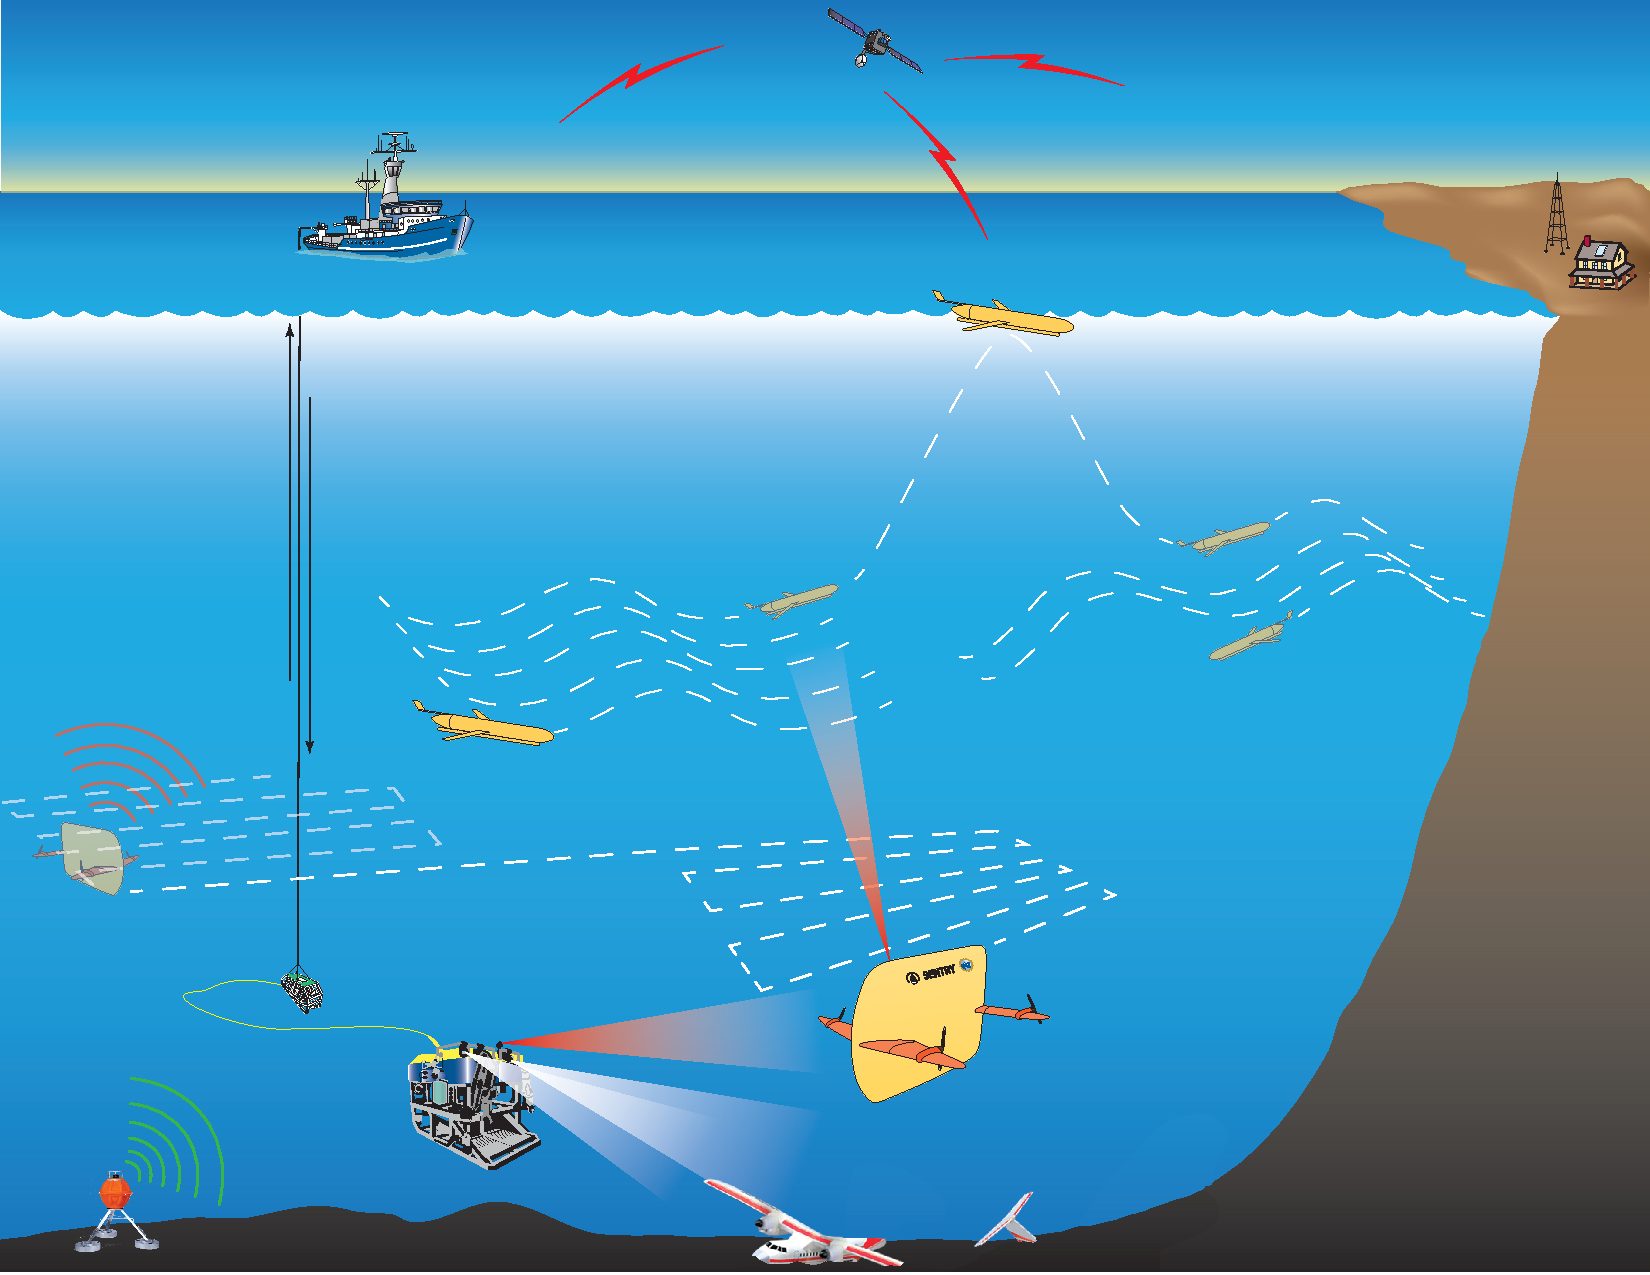
\includegraphics[width=\textwidth]{./pres/images/Adaptive4}
       \caption{Recent advances in \acf{UV} systems have enabled
         scientists and engineers to consider complex, multifaceted
         \ac{UV} missions previously thought impractical or
         impossible.  These new missions include \ac{UV} teams for
         environmental monitoring, such as the team of 5 gliders
         shown; ship-based or on-shore operator monitoring and
         re-tasking of \acp{UV}, such as the re-tasking of the
         \ac{AUV} Sentry shown; and deployment of \acp{UV} in delicate
         or dynamic environments, such as the \ac{ROV} Jason operating
         near the plane wreck shown.  {\it Improved state estimation}
         algorithms can increase navigation accuracy and lower the
         cost of \acs{UV} teams.  {\it Improved parameter
           identification} algorithms enable remote operators to
         remotely diagnose failures and use forward simulation for
         in-situ mission re-planning for \acp{UV} similar to Sentry.
         {\it Improved control} algorithms enable increased precision
         of delicate or dynamic 6-\acs{DOF} operation for \acp{ROV}
         such as Jason.  Image credit: Paul Oberlander, WHOI. }
\label{chIntro.fig.UVadaptive}
     \end{center}
  \end{figure}
\end{center}


Salt water covers over 70 \% of the surface of the earth.  
%
The world's oceans and seas to exert a huge influence on
global weather patterns, cover the longest mountain range in the
world, span 98\% of the earth's inhabitable volume, and contain
several millennia of ship wrecks.
%
Recent advances in \acf{UV} capabilities have enabled climatologists,
geologists, biologists, and archaeologists to consider addressing
research topics previously thought impractical or impossible (see
Figure \ref{chIntro.fig.UVadaptive} for examples).
%
The goal of this Thesis is to enable better utilization of these
capabilities through the development of novel algorithms for state
estimation, parameter identification, and control.
%
To this end, each type of algorithm presented herein has its own
motivating applications:
%
\begin{itemize}
%
\item {\bf State Estimation:}
%
New state estimation algorithms have the potential to improve \ac{UV}
navigation for a wide range of applications.
%
\acp{UV} operate in an environment with available sensing modalities
different from terrestrial, aerial, and on-orbit systems.
%
One consequence of these \ac{UV} specific conditions is a reliance on
dead-reckoning algorithms for translational position estimates
during 6-dimensional maneuvers.
%
It is plausible that state estimation algorithms which leverage the
group structure rigid-body motion can increase navigation
accuracy during \ac{UV} operation.
%
Such state estimation algorithms have the potential to enable \ac{UV}
navigation with different sensor suites than currently required.
%a subset of the sensor signals currently required.
%
\item {\bf Parameter Identification:} 
%
Knowledge of \ac{UV} plant parameters enable utilization of
forward simulation and other model-based algorithms for a wide range
of oceanographic research deployments.
%
The most commonly employed plant models for underwater vehicles are
finite dimensional lumped-parameter approximate models with
vehicle-specific plant parameter terms including mass and added mass
parameters; quadratic drag parameters; and gravity and buoyancy
parameters.  
%
For real-world vehicles it is impossible to compute these
plant parameters analytically, thus the plant parameters must be
identified experimentally.
%
Most previous studies of non-adaptive plant parameter identification
employ off-line conventional least-square methods requiring
instrumentation of the vehicle attitude; linear and angular velocity;
linear and angular acceleration; and applied force and moment.
%
Since \acp{UV} are often not instrumented to measure angular
acceleration, adaptive methods may provide model parameter estimates
that could not be obtained by other standard methods, such as
conventional least squares.
%
Previous adaptive parameter identification methods have focused on
model-based adaptive tracking controllers; however these approaches
are not applicable when the plant is either uncontrolled, under
open-loop control, or using any control law other than a specific
adaptive tracking controller.
%
Such conditions frequently occur on oceanographic research \ac{UV}.
%
With commercially available vehicles, often the user can not replace
the controller provided by the vehicle's manufacturer with an adaptive
tracking control algorithm.
%
Vehicle designers frequently utilize \ac{UV} passive stability of
pitch and roll in the design of under-actuated vehicles.
%
Adaptive tracking controllers assume actuation in all
degrees-of-freedom, making adaptive tracking control inapplicable for
either control or model identification of under-actuated vehicles.
%
Adaptive identification algorithms do not require simultaneous
reference trajectory-tracking control, nor do they require
instrumentation of linear acceleration or angular acceleration.

\item{\bf Trajectory-Tracking:} 
%
Many of the missions recently enabled by advances in \ac{UV}
technology, such as seafloor surveying and environmental
monitoring, depend on tracking a specified trajectory as closely as
possible.
%
To facilitate these missions, novel \ac{UV} control algorithms are
required to provide improved trajectory-tracking precision.
%
Previous studies have shown experimentally that \acl{MBC} can provide
significant performance gains over \acl{PDC}\cite{martinID_ICRA13,
smallwood2004JOE}. 
%
For most \acp{UV} the drag parameters and mass parameters (which include
both the characteristics of the vehicle's mass and those of the
ambient fluid surrounding the vehicle) can not be computed
analytically.
%
Adaptive model-based control removes the need for {\it a-priori}
parameter estimates and could enable accurate long duration trajectory
tracking through continuous model retuning.
%
\end{itemize}




% A second 

%  is to add to the toolbox of algorithms
% available for this research.
% %

% operationally relevent trajectories; 


% better 
% %


% state estimates

% This thesis 

% State observers
% %
% Picture of Jason
% %
% Picture of Nereus
% %

% low cost sensors - does not apply

% something about applying techniques from geometry control, 



% We are developing
% adaptive modeling techniques which model drag, buoyancy, inertia and
% hydrodynamic forces.  These methods 'learn' the correct parameter
% values either independently or as part of the control process.  We
% believe these methods will significantly improve UUV effectiveness for
% scientific research.


% model identification can aid 

% The Goal of this thesis is 

% use recent advances in geometric control, robotics, and ____ to develop algorithms 
%roadmap.tex
\section{Thesis Outline}


The main contributions of this Thesis are presented in Chapters
\ref{chSMS_ID}, \ref{chUV_AID}, and \ref{chUV_AMBC}.
%
A stability analysis for each novel result is included.


\noindent{\bf Chapter \ref{chModels} - Modeling Second-Order
  Mechanical Systems:} This Chapter defines the notation, functions,
state representations, and second-order plant models used in this
Thesis.


\noindent{\bf Chapter \ref{chSMS_ID} - State Estimation
  and Parameter Identification for Simple Mechanical Systems (\acs{SMS}):}
The standard models for \ac{UV} dynamic operation evolve on the set of
rigid-body transformations, SE(3).  Thus, the first third of this
Thesis is focused on utilizing the group structure of SO(3) and SE(3)
in the development of one state observer and two \ac{AID} algorithms
for \ac{SMS}.
%
These results are the theoretical antecedents of the \ac{UV} results
reported in Chapters \ref{chUV_AID} and \ref{chUV_AMBC}.
%
The plant of the angular velocity observer is a 3-\ac{DOF}
second-order rigid-body rotating under the influence of an externally
applied torque.
%
Numerical simulations of the novel angular velocity observer and two
previously reported observers are included.
%
The simulation results show similar performance of all three observers
for most angular position trajectories and inertia tensors.
%
A novel \ac{AID} algorithm is reported for a 3-\ac{DOF}
second-order rigid body rotating under the influence of an externally
applied torque, along with a simulation study.
%
An \ac{AID} algorithm for \acp{OKC} is also reported.


\noindent{\bf Chapter \ref{chUV_AID} - Adaptive Identification (\acs{AID}) for
  Underwater Vehicles (\acs{UV}):}
The \ac{UV} \ac{AID} algorithms reported herein estimate the plant
parameters for hydrodynamic mass, quadratic drag, gravitational force,
and buoyancy for a second-order rigid-body plant under the
influence of actuator forces and torques.
%
An experimental comparison of \ac{AID} and conventional
\ac{LS} %least squares parameter identification 
is reported.
%
The experimental results corroborate the analytic stability analysis,
showing that the adaptively estimated plant parameters are stable and
converge to values that provide plant-model input-output behavior
closely approximating the input-output behavior of the actual
experimental \ac{UV}.
%
The \acp{AIDPM} are shown to be similar to the \acp{LSPM} in their
ability to match the actual vehicle's input-output characteristics.



\noindent{\bf Chapter \ref{chUV_AMBC} - Adaptive Model-Based Control
  For Underwater Vehicles :}
This Chapter reports two tracking controllers: a \ac{UV} \ac{MBC}
algorithm which provides asymptotically exact trajectory-tracking, and
a novel \ac{UV} \ac{AMBC} algorithm which provides asymptotically
exact trajectory-tracking while estimating the parameters for
hydrodynamic mass, quadratic drag, gravitational force, and buoyancy
parameters for a fully-coupled second-order rigid-body \ac{UV} plant
model.

A comparative experimental evaluation of \ac{PDC} and
\ac{AMBC} for \acp{UV} is reported.
%
To the best of the author's knowledge, this is the first such
evaluation of model-based adaptive tracking control for underwater
vehicles during simultaneous dynamic motion in all 6-\ac{DOF}.
%
This experimental evaluation revealed the presence of unmodeled
thruster dynamics arising during reversals of the vehicle's thrusters,
and that the unmodeled thruster dynamics
%these short duration, small magnitude unmodeled deviations from the
%  commanded input 
can destabilize parameter adaptation.
%
The three major contributions of this experimental evaluation are: an
experimental analysis of how unmodeled thruster dynamics can
destabilize parameter adaptation, a two-step adaptive model-based
control algorithm which is robust to the thruster modeling errors
present, and a comparative experimental evaluation of \ac{AMBC} and
\ac{PDC} for fully-actuated underwater vehicles
preforming simultaneous 6-\ac{DOF} trajectory-tracking.



\noindent{\bf Chapter \ref{chConc} - Conclusion:}
Thesis results summarized and directions for future work presented.



\noindent{\bf Appendix \ref{appenJHUHTF} - Johns Hopkins University
  Hydrodynamic Test Facility:}
The details of the Johns Hopkins University Hydrodynamic Test Facility
and our experimental testing methodologies are presented.
%
This facility includes the \ac{JHUROV}, a fully actuated \ac{UV} used
for the experimental trials reported in Chapters \ref{chUV_AID} and
\ref{chUV_AMBC}.



\noindent{\bf Appendix \ref{appenJacSE3} - Special Euclidean Group
  Velocity Jacobian:}
Details of the SE(3) Velocity Jacobian are reported.  These results
are required for the \ac{UV} \ac{MBC} stability proof (Theorem
\ref{chUV_AMBC.theo.UV_MBC}).
%


%say something like: 

%Using  currently being preformed
%between PD control, non-adaptive model-based control and adaptive
%model-based control for a number of trajectories including set-point
%control, single degree-of-freedom motion, planar motion and
%simultaneous six-degree-of-freedom motion.  To the best of my
%knowledge, this will be the first set of experiments to identify
%classes of maneuvers where \ac{UV} operators can expect to see
%performance gains from adaptive model based control.

%\chapter{Modeling Second Order Mechanical Systems}
\chapter{Modeling Second-Order Rigid-Body Mechanical Systems}
\label{chModels}
\chaptermark{Modeling Second-Order Mechanical Systems}

%\ssp
\acresetall

%Some of this work was orginally published in ...
% \textit{ACM Transactions on Applied Perception} in 2010 with
% co-authors A.\ M.\ Okamura and K.\ J.\ Kuchenbecker
% \cite{Blank_TAP2010}.  Some additional material has been added here
% for clarity.


%\section{Introduction}
%\label{chModels.sec.intro}

This Chapter summarizes the notation, kinematic conventions, and plant
models used in this Thesis.
%
With the exception of Section \ref{chModels.sec.genMat_Factorization},
the models, functions, state spaces, and facts stated herein are commonly
employed in the fields of geometric control,
adaptive control, and  underwater robotics. 
%
Section \ref{chModels.sec.notation} states the functions, norms, and
\ac{SPD} matrix eigenvalue conventions used herein.
%
Section \ref{chModels.sec.genMat_Factorization} reports a proof of
Theorem \ref{chModels.theo.diagMat_Factorization}, which allows
general 3-by-3 matrices to be factored through the skew symmetric
operator.
%
Sections \ref{chModels.sec.SO3} and \ref{chModels.sec.SE3} detail
the position and velocity state representations used herein for a
rotating rigid-body and general rigid-body motion.
%
The analytic relationships between these state representations are
also stated.
%
This Chapter presents second-order models for:
\begin{itemize}
\item 3-\ac{DOF} rotating rigid-body dynamics (Section \ref{chModels.sec.SO3plant}), 
\item 3-\ac{DOF} rotating \ac{UV} dynamics  (Section \ref{chModels.sec.UVSO3plant}), 
\item 6-\ac{DOF} \ac{UV} dynamics (Section \ref{chModels.sec.UVSE3plant}), and 
\item {\it n}-link \ac{OKC} dynamics (Section \ref{chModels.sec.OKC}).
\end{itemize}
%
For each of the four models, plant parameter properties and the
model's regressor matrix factored form are also presented.
%
Readers seeking a presentation of this material in greater detail are
referred to the texts cited in Section \ref{chModels.sec.litReview}.


As noted in the summery above, we believe Theorem
\ref{chModels.theo.diagMat_Factorization} is a novel result.
%
This Theorem states that $A^T((Ax)\times(Ay))=\det(A)(x\times y)$ for
all $A\in\rSp{3\times 3}$ and $x,y\in\rSp{3}$, where $\times$ is the
usual cross product operator for $\rSp{3}$ and $\det(\cdot)$ is the
matrix determinate.
%
This result is a generalization of the well known fact $(Rx)\times y=
R(x\times(Ry))$ for all $x,y\in\rSp{3}$ and $R\in\SO3$, where SO(3) is
the special orthogonal group for $\rSp(3)$.
%
To the best of our knowledge, this relation has not been proposed or
proven previously.



\section{Background Literature}
\label{chModels.sec.litReview}

%The priciple foundation literature on which this Thesis builds
%includes the following:
%
The foundation of this Thesis is a set of good ideas and facts cherry
picked from the long history of research into modeling rigid-body
dynamics.
%
Those ideas and facts are summarized in this Chapter.
%
Readers requiring more information are referred to the following texts
for the reasons listed.
%
Taylor's {\it Classical Mechanics}\cite{Taylor2005} provides an
excellent introduction to modeling rigid-body motion using
non-inertial reference frames.
%
In \cite{Bullo2004}, Bullo and Lewis provide both a rigorous
development of and a compelling case for utilizing differential
geometry techniques in nonlinear control theory.
%
Chapters 5, 6, and 7 from \cite{Chirikjian2000}, by Chirikjian and
Kyatkin, and \cite{murray&li&sastry}, by Murray, Li and Sastry,
elucidate the representation of rigid-body motion in the groups SO(3)
and SE(3).
%
{\it A Short Introduction to Applications of Quaternions}, by
A. G. Rawlings\cite{RawlingQuaternions}, presents different coordinate
systems used to represent rigid-body rotations.
%
Rawlings's text also presents the intuition behind the individual
coordinate systems and the interconnections between those
representations.
%
{\it Guidance and Control of Ocean Vehicles} by
Fossen\cite{fossen} and {\it Advances in Six-Degree-of-Freedom
  Dynamics and Control of Underwater Vehicles} by
Martin\cite{martin.thesis} present the details of modeling \acf{UV}
dynamics.



\section{Notation Conventions}
\label{chModels.sec.notation}

We assume the readers are familiar with SO(3), the special orthogonal
group for $\rSp{3}$, and SE(3), the special euclidean group for
$\rSp{3}$.  We also assume readers are familiar with their tangent
spaces so(3) and se(3) respectively.  Readers not familiar with these
concepts are referred to \cite{murray&li&sastry}.

\subsection{Function Definitions}
\label{chModels.sec.functionDefn}

\noindent Functions used throughout this text are defined as follows:
%
\begin{itemize}
\item $\mathcal{J}:\mathbb{R}^3\to\mathbb{R}^{3\times 3}$ is
the mapping from $\realSpace{3}$ to so(3), the tangent space of SO(3),
and is defined by
%
\begin{equation}
\mathcal{J}\left(
\left[ \begin{array}{c} 
\omega_1 \\\omega_2  \\ \omega_3 \\
\end{array} \right]\right) =
\left[ \begin{array}{ccc}
     0     & -\omega_3 &  \omega_2                               \\
   \omega_3  &    0    & -\omega_1                               \\
  -\omega_2  &  \omega_1 &    0                                  \\
\end{array} \right].
\end{equation}
%
%
\item $\widehat{\cdot}:\mathbb{R}^6\to\mathbb{R}^{4\times 4}$ is the
  mapping from $\mathbb{R}^6$ to se(3), the tangent space of SE(3),
  and (for $\nu,\omega\in\rSp{3}$) is defined by
%
\begin{equation}
\widehat{
\left[ \begin{array}{c} 
\nu \\ \omega  \\
\end{array} \right] } =
\left[ \begin{array}{cc}
     \mathcal{J}(\omega) & \nu        \\
        0_{1 \times 3}     &  0         \\
\end{array} \right].
\end{equation}
%
%
\item $\ad:\mathbb{R}^6\to\mathbb{R}^{6\times 6}$ is the se(3) adjoint
operator. For the vector 
%
\begin{equation}
v=\left[ \begin{array}{c} 
\nu \\ \omega  \\
\end{array} \right]
\end{equation} 
%
the se(3) adjoint operator is defined as
%
\begin{equation}
\label{chModels.eq.ad}
\ad_v=
\left[ \begin{array}{cc}
     \mathcal{J}(\omega) &  \mathcal{J}(\nu)        \\
      0_{3 \times 3}     & \mathcal{J}(\omega)    \\
\end{array} \right].
\end{equation}
%
%
\item $\Ad:\SE3\to\mathbb{R}^{6\times 6}$ is the se(3) adjoint map,  defined as
%
\begin{equation}
\label{chModels.eq.Ad}
\Ad\left(
\left[ \begin{array}{cc} 
R &  p \\ 
0_{1\times 3} &  1 \\
\end{array} \right]\right) =
\left[ \begin{array}{cc}
             R           & \mathcal{J}(p) R   \\
      0_{3 \times 3}        &    R  \\
\end{array} \right].
\end{equation}
%
%
\item \funDefn{\otimes}{\realSpace{m\times n}\times\realSpace{p\times q}}{\realSpace{(m*p)\times (n*q)}}
is the Kronecker product operator\cite{kron}.  
%
For matrices 
%
\begin{equation}
A=\left[ \begin{array}{cccc} 
a_{11} & a_{12} &\hdots & a_{1n}  \\
a_{21} & a_{22} &       & a_{2n}  \\
\vdots &      &\ddots & \vdots \\
a_{m1} & a_{m2} &\hdots & a_{mn}  \\
\end{array} \right]
%
\text{ and }
%
B=\left[ \begin{array}{cccc} 
b_{11} & b_{12} &\hdots & b_{1q}  \\
b_{21} & b_{22} &       & b_{2q}  \\
\vdots &      &\ddots & \vdots \\
b_{p1} & b_{p2} &\hdots & b_{pq}  \\
\end{array} \right]
\end{equation}
%
the Kronecker product is defined as
%
\vspace{5mm}
\begin{equation}
A\otimes B=\left[ \begin{array}{cccc} 
a_{11}B & a_{12}B & \hdots & a_{1n}B  \\
a_{21}B & a_{22}B &        & a_{2n}B  \\
\vdots &        & \ddots & \vdots  \\
a_{m1}B & a_{m2}B & \hdots & a_{mn}B  \\
\end{array} \right].
\end{equation}
%
%
\item \funDefn{\cdot^S}{\realSpace{m\times n}}{\realSpace{(m*n)}} is the
stack operator.  Using the definition of $A$ above, the stack operator is
defined by stacking the columns of $A$ such that  
%
\begin{equation}
A^S=\left[ \begin{array}{ccccccccccccc} 
a_{11}  &
a_{21}  &
\cdots &
a_{m1}  &
a_{12}  &
a_{22}  &
\cdots &
a_{m2}  & 
\cdots &
a_{1n}  &
a_{2n}  &
\cdots &
a_{mn}
\end{array} \right]^T.
\end{equation}
%
%\begin{equation}
%A^S=\left[ \begin{array}{c} 
%a_{11}  \\
%a_{21}  \\
%\vdots \\
%a_{m1}  \\
%a_{12}  \\
%a_{22}  \\
%\vdots \\
%a_{m2}  \\ 
%\vdots \\
%a_{1n}  \\
%a_{2n}  \\
%\vdots \\
%a_{mn}
%\end{array} \right].
%\end{equation}
\end{itemize}
%
This Thesis will also make use of 
%
\begin{itemize}
\item the SO(3) exponential map, \funDefn{\e_{\SO3}}{\so3}{\SO3} 
\item the SO(3) logarithmic map, \funDefn{\log_{SO3}}{\SO3}{\so3}
\item the SE(3) exponential map, \funDefn{\e_{\SE3}}{\se3}{\SE3} 
\item the SE(3) logarithmic map, \funDefn{\log_{SE3}}{\SE3}{\se3}
\end{itemize}
% 
See \cite{murray&li&sastry} for additional information, including
closed form functions, for these maps.

\subsection{Vector Norm, Matrix Norm, and Eigenvalue  Conventions}
\label{chModels.sec.normConventions}

Let $M\in\mathbb{R}^{n\times n}$ represent a \ac{SPD} inertia tensor
or hydrodynamic mass matrix. Note that the eigenvalues of symmetric
matrices are always real.  This Thesis employs the following
conventions for the eigenvalues of such matrices: $m_n$ is the
smallest and $m_1$ is the largest eigenvalues of the mass matrix, the
other eigenvalues are labeled such that $m_{i-1}\leq m_i\leq
m_{i+1}$ $\forall i$ such that $2\leq i\leq n-1$. This convention will also be used for any mass matrix
estimate or mass matrix error term, i.e. if $\hat{M}(t)$ is an
estimate of a true mass matrix $M$ and $\Delta M(t)=\hat{M}(t)-M$ then
these eigenvalues will be ordered such that $\hat{m}_{i-1}(t)\leq
\hat{m}_i(t) \leq \hat{m}_{i+1}(t)$ and $\Delta m_{i-1}(t)\leq \Delta
m_i(t) \leq \Delta m_{i+1}(t)$. We assume that the eigenvalues of
physically realistic mass matrices are either constant or bounded for
all time, i.e. there exists a scalar $a\in\mathbb{R}_+$ such that
$m_1<a$.



The $\ell 2$ norm, or Euclidean norm, for $x\in\mathbb{R}^n$ is
defined as $\|x\|=\left(\sum_{i=1}^n x_i^2\right)^{1/2}$.  The $\ell 2$ induced
matrix norm, also known as the spectral norm, for $M\in\mathbb{R}^{n
  \times n}$ is defined as $\|M\|_2=\max_{\|x\|=1}\|Mx\|$.  Let
$a_{ij}$ be the individual entries of $A\in\mathbb{R}^{n\times n}$,
the Frobenius norm of $A$ is defined as
$\|A\|_F=\left(\sum_{i,j=1}^n|a_{ij}|^{2} \right)^{1/2}$.  For more
information on these norms see \cite{horn&johnson}. We define the
following matrix semi-norm
%
\begin{equation}
\minNorm{M}=\min_{\|x\|=1}\|Mx\|.
\end{equation}
%
For a given mass matrix $M$, these definitions and the cross product
property $\|x_1\times x_2\|\leq \|x_1\|\|x_2\|$ give rise to the
following properties

\begin{align}\label{chModels.eq.AVO_ineq}
  m_n\|x\|&=\minNorm{M}\|x\|\leq\|Mx\|\leq\|M\|_2\|x\|=m_1\|x\|, 
   \\
  \|-Mx\|&\leq-m_n\|x\|,
   \\
  \|M^{-1/k}\|_2&=\|M^{-1}\|_2^{1/k}=\left(\frac{1}{m_n}\right)^{1/k},
   \\
  \|M L\|_2&\leq\|M\|_2\|L\|_2=m_{1} l_{1},~ \text{and} 
   \\ 
  \|\mathcal{J}(M x_1)x_2\|&\leq\|M x_1\|\|x_2\|\leq m_1\|x_1\|\|x_2\|.
\end{align}



%\subsection{\acl{SPD} Matrix Factorization Through the Skew 
  Symmetric Operator}
% factorization is the decomposistion of an object (e.g. a number, a
% polynomial or a matrix) into the product of other objects, or
% factors, which when multiplied together give the original.
%
% Jon B. like the title for this lemma of "Positive Definite Symmetric
% Skew Symmetric Factorization" which should be abbreviated "PDS3
% Factorization" according to him

\newtheorem{PDS3_Factorization}{Lemma}[section]

\begin{PDS3_Factorization}
\label{chModels.theo.PDS3_Factorization}
For all $a,b,c,d\in\mathbb{R}$, $x\in\mathbb{R}^3$, and $I$ such that
$I\in\realSpace{3\times 3}$ and $I$ is \ac{SPD}, the following
equality holds

\begin{equation}
\label{chModels.eq.PDS3_Factorization}
I^a\mathcal{J}\left(I^b x\right)I^c=\det(I)^d I^{a-d}\mathcal{J}
\left(I^{b-d} x\right)I^{c-d}.
\end{equation}

\end{PDS3_Factorization}

\noindent Proof:

First lets develop a factorization of $\soThreeMap{Dx}$, where
$D\in\realSpace{3\times 3}$ is a \ac{SPD} diagonal matrix with
diagonal terms $\lambda_1,\lambda_2,\lambda_3>0$ and
$x\in\mathbb{R}^3$ is a vector with terms
$x_1,x_2,x_3\in\realSpace{}$.  Note that For all $d\in\mathbb{R}$ we
have the equaltity
$\det\left(D\right)^d=\det\left(D^d\right)=\lambda_1^d\lambda_2^d\lambda_3^d$,
thus


\begin{align}
\det(D)^d& D^{-d}\mathcal{J}(x) D^{-d}
\nonumber \\
   =&\det(D^d)
    \left[ \begin{array}{ccc}
      \lambda_1^{-d}  &      0           &      0               \\
          0          &   \lambda_2^{-d}  &      0               \\
          0          &      0           & \lambda_3^{-d}        \\
    \end{array} \right]
    \left[ \begin{array}{ccc}
         0    & -x_3 &  x_2                               \\
         x_3  &   0  & -x_1                               \\
        -x_2  &  x_1 &    0                               \\
    \end{array} \right]
    \left[ \begin{array}{ccc}
      \lambda_1^{-d}  &      0           &      0               \\
          0          &   \lambda_2^{-d}  &      0               \\
          0          &      0           & \lambda_3^{-d}        \\
    \end{array} \right]
   \nonumber \\
   =&\lambda_1^d\lambda_2^d\lambda_3^d
    \left[ \begin{array}{ccc}
         0  &  -\lambda_1^{-d}\lambda_2^{-d}x_3  &  \lambda_1^{-d}\lambda_3^{-d}x_2     \\
          \lambda_1^{-d}\lambda_2^{-d}x_3  &  0  &  -\lambda_2^{-d}\lambda_3^{-d}x_1    \\
         -\lambda_1^{-d}\lambda_3^{-d}x_2  &  \lambda_2^{-d}\lambda_3^{-d}x_1 &    0    \\
    \end{array} \right]
   \nonumber \\
   =&
    \left[ \begin{array}{ccc}
         0  &  -\lambda_3^d x_3  &  \lambda_2^d x_2     \\
          \lambda_3^d x_3  &  0  &  -\lambda_1^d x_1    \\
         -\lambda_2^d x_2  &  \lambda_1^d x_1 &    0    \\
    \end{array} \right]
   \nonumber \\
   =&\mathcal{J}\left(D^d x \right)
\end{align}

\noindent Next, consider (\ref{chModels.eq.PDS3_Factorization}). Let $\lambda_1$,
$\lambda_2$ and $\lambda_3$ be the eigenvalues of $I$, where the
$\lambda_i$ are labeled without regard to ordering for the largest or
smallest eigenvalues. Since $I$ is \ac{SPD}, these eigenvalues are
positive and there exists a $R\in\SO3$ and \ac{SPD} diagonal matrix
$D\in\mathbb{R}^{3 \times 3}$ such that $\lambda_1$, $\lambda_2$ and
$\lambda_3$ are the diagonal terms of $D$ and $I=RDR^T$. Note that for
$d\in\mathbb{R}$ we have the equality
$\det(I)^d=\det(D)^d=\lambda_1^d\lambda_2^d\lambda_3^d$ and for all
$R\in\SO3$ we have the equality
$R\mathcal{J}\left(x\right)R^T=\mathcal{J}\left(Rx\right)$, thus

\begin{align}
I^a\mathcal{J}\left(I^b x\right)I^c
  =& RD^aR^T\mathcal{J}\left(RD^bR^T x\right)RD^cR^T
\nonumber \\
  =& RD^a\mathcal{J}\left(D^bR^T x\right)D^cR^T
\nonumber \\
  =& RD^a\mathcal{J}\left(D^dD^{b-d}R^T x\right)D^cR^T
\nonumber \\
  =& RD^a\left(\det\left(D^d\right)D^{-d}\mathcal{J}\left(D^{b-d}R^T x\right)D^{-d}\right)D^cR^T
\nonumber \\
  =&\det\left(I^d\right) RD^{a-d}\mathcal{J}\left(D^{b-d}R^T x\right)D^{c-d}R^T
\nonumber \\
  =&\det\left(I^d\right) RD^{a-d}R^T\mathcal{J}\left(R D^{b-d}R^T x\right)RD^{c-d}R^T
\nonumber \\
  =&\det\left(I^d\right) I^{a-d}\mathcal{J}\left(I^{b-d} x\right)I^{c-d}.
\nonumber \\
\end{align}

This completes the proof. In the following chapters Lemma
\ref{chModels.theo.PDS3_Factorization} is not explicitly used, but its
existence has been beneficial in developing Lyapunov functions for
second-order rotational plants.

\section{Matrix Factorization Through the \\Skew
  Symmetric Operator}
% factorization is the decomposistion of an object (e.g. a number, a
% polynomial or a matrix) into the product of other objects, or
% factors, which when multiplied together give the original.
%
% Jon B. like the title for this lemma of "Positive Definite Symmetric
% Skew Symmetric Factorization" which should be abbreviated "PDS3
% Factorization" according to him
\label{chModels.sec.genMat_Factorization}


\begin{realOrth_Factorization}
\label{chModels.theo.realOrth_Factorization}
For all real orthogonal matrices  $U\in\O3$ and $a\in\rSp{3}$ the
following equality holds
%
\begin{equation}
\label{chModels.eq.realOrth_Factorization}
U\soThreeMap{x}U^T=\det(U)\soThreeMap{Ua}
\end{equation}
%
\end{realOrth_Factorization}
%
\noindent Proof: Let $x,y,z\in\rSp{3}$ be defined such that
%
$U^T=\left[x \quad y \quad z \right]$.
%$
%U^T=
%\left[ \begin{array}{ccc}
%  x  &
%  y  &
%  z  
%\end{array} \right].
%$ 
%
The facts $UU^T=\mathbb{I}$ and $x^T\soThreeMap{y}z=\det(U)$
imply that $\soThreeMap{y}z=\det(U)x$,
$\soThreeMap{z}x=\det(U)y$, and $\soThreeMap{x}y=\det(U)z$.
%
Note that $\forall\;\psi_1,\psi_2,a\in\rSp{3}$ we know
$\psi_1^T\soThreeMap{a}\psi_2=a^T\soThreeMap{\psi_2}\psi_1$ and consider
%
\begin{align}
U\soThreeMap{a}U^T
%  =&U \left[ \soThreeMap{a}x\;\;\soThreeMap{a}y\;\;\soThreeMap{a}z\right]
  =&U \left[\begin{array}{ccc}\soThreeMap{a}x&\soThreeMap{a}y&\soThreeMap{a}z\end{array}\right]
\nonumber \\
  =&\left[
\begin{array}{ccc}
  x^T\soThreeMap{a}x  & x^T\soThreeMap{a}y  & x^T\soThreeMap{a}z  \\
  y^T\soThreeMap{a}x  & y^T\soThreeMap{a}y  & y^T\soThreeMap{a}z  \\
  z^T\soThreeMap{a}x  & z^T\soThreeMap{a}y  & z^T\soThreeMap{a}z  \\
\end{array} \right]
\nonumber \\
  =&\left[
\begin{array}{ccc}
          0           & a^T\soThreeMap{y}x  & a^T\soThreeMap{z}x  \\
  a^T\soThreeMap{x}y  &           0         & a^T\soThreeMap{z}y  \\
  a^T\soThreeMap{x}z  & a^T\soThreeMap{y}z  &         0           \\
\end{array} \right]
\nonumber \\
  =&\soThreeMap{\left[\begin{array}{ccc}a^T\soThreeMap{y}z \\a^T\soThreeMap{z}x \\a^T\soThreeMap{x}y \\\end{array} \right]}
\nonumber \\
 =&\det(U)\soThreeMap{Ua}
\end{align}
%


\begin{diagMat_Factorization}
\label{chModels.theo.diagMat_Factorization}
For all diagonal matrices $D\in\rSp{3\times 3}$ and $x\in\rSp{3}$ the
following equality holds

\begin{equation}
\label{chModels.eq.diagMat_Factorization}
D\soThreeMap{Dx}D=\det(D)\soThreeMap{x}
\end{equation}

\end{diagMat_Factorization}

\noindent Proof:
%
Let $\lambda_1,\lambda_2,\lambda_3\in\rSp{}$ be the diagonal entries 
of $D$ and $x_1,x_2,x_3\in\realSpace{}$ be the entries of 
$x\in\mathbb{R}^3$.
%
Note that we have the equality
$\det\left(D\right)=\lambda_1\lambda_2\lambda_3$,
thus


\begin{align}
D\soThreeMap{Dx} D
   =&\
    \left[ \begin{array}{ccc}
      \lambda_1  &      0           &      0               \\
          0          &   \lambda_2  &      0               \\
          0          &      0           & \lambda_3        \\
    \end{array} \right]
    \left[ \begin{array}{ccc}
               0       & -\lambda_3 x_3 &  \lambda_2 x_2    \\
         \lambda_3 x_3  &    0          & -\lambda_1 x_1    \\
        -\lambda_3 x_2  &  \lambda_3x_1 &    0              \\
    \end{array} \right]
    \left[ \begin{array}{ccc}
      \lambda_1      &      0           &      0           \\
          0          &   \lambda_2      &      0           \\
          0          &      0           & \lambda_3        \\
    \end{array} \right]
   \nonumber \\
   =&
    \left[ \begin{array}{ccc}
                       0  &  -\lambda_1\lambda_2\lambda_3x_3  &  \lambda_1\lambda_2\lambda_3x_2     \\
          \lambda_1\lambda_2\lambda_3x_3  &          0        &  -\lambda_1\lambda_2\lambda_3x_1    \\
         -\lambda_1\lambda_2\lambda_3x_2  &  \lambda_1\lambda_2\lambda_3x_1 &    0    \\
    \end{array} \right]
   \nonumber \\
   =&\lambda_1\lambda_2\lambda_3
    \left[ \begin{array}{ccc}
         0  &  -x_3  &  x_2     \\
         x_3  &  0  &  -x_1    \\
        -x_2  &  x_1 &    0    \\
    \end{array} \right]
   \nonumber \\
   =&\det(D)\soThreeMap{x}
\end{align}


\begin{genMat_Factorization}
\label{chModels.theo.genMat_Factorization}
For all matrices $A\in\rSp{3\times 3}$ and $x\in\rSp{3}$ the
following equality holds

\begin{equation}
\label{chModels.eq.genMat_Factorization}
A^T\soThreeMap{Ax}A=\det(A)\soThreeMap{x}
\end{equation}

\end{genMat_Factorization}

Proof:
%
Consider the following facts
%
\begin{itemize}
%
\item From Lemma \ref{chModels.theo.diagMat_Factorization}, $U\in\O3$, and
  $x\in\rSp{3}$ we know $\soThreeMap{U x}=\det(U) U\soThreeMap{x}U^T$.
\item From Lemma \ref{chModels.eq.diagMat_Factorization}, for all
  diagonal matrices $\Sigma\in\rSp{3\times 3}$, and all $x\in\rSp{3}$
  we know $\Sigma^T\soThreeMap{\Sigma}\Sigma=\det(\Sigma)\soThreeMap{x}$.
%
\item For all $A\in\rSp{3\times 3}$ there exists an SVD decomposition
  for which $A=U\Sigma V^T$ where $U\in\rSp{3\times 3}$ and
  $V\in\rSp{3\times 3}$ are real orthogonal matrices, and
  $\Sigma\in\rSp{3\times 3}$ is a diagonal matrix with the singular
  values of $A$ along its diagonal.
%
\item $\det(A)=\det(U)\det(\Sigma)\det(V)$.
%
\end{itemize}
%
Thus
%
\begin{align}
A^T\soThreeMap{Ax}A&=V \Sigma U^T \soThreeMap{U \Sigma V^T x} U \Sigma V^T
\nonumber \\
&=\det(U)V \Sigma U^TU \soThreeMap{\Sigma V^T x}U^TU\Sigma V^T
\nonumber \\
&=\det(U)V \Sigma \soThreeMap{\Sigma V^T x}\Sigma V^T
\nonumber \\
&=\det(U)\det(\Sigma) V \soThreeMap{V^T x} V^T
\nonumber \\
&=\det(U)\det(\Sigma)\det(V) V V^T \soThreeMap{x}V V^T
\nonumber \\
&=\det(A)\soThreeMap{x}
\end{align}



\begin{PDS3_Factorization}
\label{chModels.theo.PDS3_Factorization}
For all $a,b,c,d\in\mathbb{R}$, $x\in\mathbb{R}^3$, and 
$I\in\realSpace{3\times 3}$ such that $I$ is \ac{SPD}, the following
equality holds
%
\begin{equation}
\label{chModels.eq.PDS3_Factorization}
I^a\mathcal{J}\left(I^b x\right)I^c=\det(I)^d I^{a-d}\mathcal{J}
\left(I^{b-d} x\right)I^{c-d}.
\end{equation}
%
\end{PDS3_Factorization}
%
Proof: Let $\lambda_1$, $\lambda_2$ and $\lambda_3$ be the eigenvalues
of $I$, where the $\lambda_i$ are labeled without regard to ordering
for the largest or smallest eigenvalues. Since $I$ is \ac{SPD}, these
eigenvalues are positive and there exists $R\in\SO3$ and \ac{SPD}
diagonal matrix $D\in\mathbb{R}^{3 \times 3}$ such that $\lambda_1$,
$\lambda_2$ and $\lambda_3$ are the diagonal terms of $D$ and
$I=RDR^T$. Note that for $d\in\mathbb{R}$ we have the equality
$\det(I)^d=\det(D)^d=\lambda_1^d\lambda_2^d\lambda_3^d$, from Lemma
\ref{chModels.theo.diagMat_Factorization} we know $\det(D)^d
D^{-d}\mathcal{J}(x) D^{-d}=\soThreeMap{D^d x}$ and for all $R\in\SO3$
we have the equality $R\soThreeMap{x}R^T=\soThreeMap{Rx}$. Thus

\begin{align}
I^a\mathcal{J}\left(I^b x\right)I^c
  =& RD^aR^T\mathcal{J}\left(RD^bR^T x\right)RD^cR^T
\nonumber \\
  =& RD^a\mathcal{J}\left(D^bR^T x\right)D^cR^T
\nonumber \\
  =& RD^a\mathcal{J}\left(D^dD^{b-d}R^T x\right)D^cR^T
\nonumber \\
  =& RD^a\left(\det\left(D^d\right)D^{-d}\mathcal{J}\left(D^{b-d}R^T x\right)D^{-d}\right)D^cR^T
\nonumber \\
  =&\det\left(I^d\right) RD^{a-d}\mathcal{J}\left(D^{b-d}R^T x\right)D^{c-d}R^T
\nonumber \\
  =&\det\left(I^d\right) RD^{a-d}R^T\mathcal{J}\left(R D^{b-d}R^T x\right)RD^{c-d}R^T
\nonumber \\
  =&\det\left(I^d\right) I^{a-d}\mathcal{J}\left(I^{b-d} x\right)I^{c-d}.
\nonumber \\
\end{align}

This completes the proof. In the following Chapters Corollary
\ref{chModels.theo.PDS3_Factorization} is not explicitly used, but has
been useful in developing Lyapunov functions for second-order
rotational plants.

\section{State Representations}

\subsection{Rotating Rigid-Body Kinematics}
%\subsection{Special Orthogonal Group}
\label{chModels.sec.SO3}

\noindent We use three state representations of rigid-body angular
position and velocity:
\begin{itemize}
\item $q\in\mathbb{R}^3$, the angular position in so(3)
exponential coordinates,
\item $\omega\in\mathbb{R}^3$, the body-frame angular velocity, and
\item $R\in\SO3$, the rotation matrix from the body-frame to the
  world-frame.
\end{itemize}
%
The relations between these state representations are given by
%
\begin{align}
R=&e^{\mathcal{J}(q)}  \\
\dot{R}=&R\mathcal{J}(\omega).
\end{align}

%------------------old version------------------------------
% We represent the angular position of the rigid body in so(3)
% exponential coordinates as $q\in\mathbb{R}^3$ and it's angular
% velocity as $\omega\in\mathbb{R}^3$.
% %
% Angular position can also be represented as a rotation matrix
% from a body-frame to a world-frame, $R\in\SO3$.
% %
% The relations between these state representations are

% \begin{align}
% R=&e^{\mathcal{J}(q)}  \\
% \dot{R}=&R\mathcal{J}(\omega).
% \end{align}



\noindent Throughout this study we make use of the relation between
the body-frame angular velocity, $\omega$, and the time derivative of
the exponential coordinate position, $\dot{q}$, which takes the form
%
\begin{equation}
\omega=\mathcal{A}(q) \dot{q}.
\end{equation}
%
The closed form for the Jacobian \funDefn{A}{\rSp{3}}{\rSp{3\times 3}}
given by
%
\begin{equation}\label{chModels.eq.A}
A(q)=I+\left(\frac{1-\cos{\|q\|}}{\|q\|}\right)\frac{\mathcal{J}(q)}{\|q\|}+
\left(1-\frac{\sin{\|q\|}}{\|q\|}\right)\frac{\mathcal{J}(q)^2}{\|q\|^2}.
\end{equation}
%
was first reported by Park in \cite{Park1991}. The inverse of this mapping,
%
\begin{equation}
\dot{q}=\mathcal{A}^{-1}(q)\omega,
\end{equation}
%
\funDefn{A^{-1}}{\rSp{3}}{\rSp{3\times 3}} also has a closed functional
  form given by
%
\begin{equation}\label{chModels.eq.Ainv}
  \mathcal{A}^{-1}(q)=I_{3\times 3}-\frac{1}{2}\mathcal{J}(q)+\left(1-\frac{\|q\|}{2}\cot{\frac{\|q\|}{2}}\right)\frac{\mathcal{J}(q)^2}{\|q\|^2}.
\end{equation}
%
This inverse exists for $\|q\|<\pi$ \cite{Park1991}.  See
\cite{Bullo2004,Chirikjian2000} for additional properties.


\subsection{Rotating and Translating Rigid-Body Kinematics}
%\subsection{Special Euclidean Group}
\label{chModels.sec.SE3}

\noindent We use seven state representations of rigid-body pose and velocity:
\begin{itemize}
\item $\psi\in\mathbb{R}^6$, the pose in se(3) exponential
coordinates,
\item $v\in\mathbb{R}^6$, the body-frame velocity,   
\item $H\in\SE3$, the homogenious transform from the body-frame to the world-frame,
\item $R\in\SO3$, the rotation matrix from the body-frame to the
  world-frame,
\item $p\in\mathbb{R}^3$, the vector representing the body-frame's
  origin in the world-frame,
\item $\nu\in\mathbb{R}^3$, the vehicle's body-frame translational
  velocity, and
\item $\omega\in\mathbb{R}^6$, the vehicle's body-frame angular
  velocity.
\end{itemize} 
%
%Many of our analytic results rely on representing the vehicle's state
%in exponential coordinates, $\psi$, and body-frame velocity, $v$.
%
The relations between these state representations are given by
%
\begin{align}
H=&e^{\widehat{\psi}}, \\
\dot{H}=&H\widehat{v}, \\
H=&\left[ \begin{array}{cc}
         R      & p  \\
    0_{1 \times 3}  & 1  \\
  \end{array} \right],~\text{and} \\
v=&\left[ \begin{array}{c} \nu \\  \omega \\ \end{array} \right].
\end{align}
% %----------------Old Version of-------------------------------- 
% We represent the pose of the rigid body in se(3) exponential
% coordinates as $\psi\in\mathbb{R}^6$ and its body-frame velocity using
% $v\in\mathbb{R}^6$. 
% %
% Rigid body pose can also be represented as a homogenious transform 
% from the body-frame to the world-frame, $H\in\SE3$.
% %
% The relations between these state representations are
% %
% \begin{align}
% H=&e^{\widehat{\psi}} \\
% \dot{H}=&H\widehat{v}.
% \end{align}
% %
% Further, note that for $R\in\SO3$, the rotation matrix from
% the body-frame to the world-frame, and $p\in\mathbb{R}^3$, the vector
% representing the location of body-frame's origin in the world-frame,
% we have the equality
% %
% $H=\left[ \begin{array}{cc}
%          R      & p  \\
%     0_{1 \times 3}  & 1  \\
%   \end{array} \right]$.
% %
% Finally, note that for $\nu\in\mathbb{R}^3$, the vehicle's
% body-frame translational velocity, and $\omega\in\mathbb{R}^6$, the
% vehicle's body-frame angular velocity, we have the equality
% %
% $v=\left[ \begin{array}{c} \nu \\  \omega \\ \end{array} \right]$.


We employ the inverse SE(3) velocity Jacobian,
\funDefn{\hat{\mathcal{A}}^{-1}}{\rSp{6}}{\rSp{6\times 6}}, as a
relation between the body-frame velocity and time derivative of
exponential coordinate pose
%
\begin{equation}\label{chModels.eq.hatAInv}
\dot{\psi}=\hat{\mathcal{A}}^{-1}(\psi) v.
\end{equation}
%
In \cite{bullo1995_SE3_PD} the authors derive a closed form expression
for this matrix valued function, reprinted in Appendix
\ref{appenJacSE3} as (\ref{appenJacSE3.eq.hatAinv}).
%
To the best of the author's knowledge a closed form expression for the
SE(3) angular velocity Jacobian, $\hat{\mathcal{A}}\left(\psi\right)$,
has not been reported.
%
Appendix \ref{appenJacSE3} provides further information on this
Jacobian, including the derivation of a simpler closed form
(\ref{appenJacSE3.eq.hatAinv2}), proof that
$\psi^T\left(\hat{\mathcal{A}}^{-T}(\psi)+\hat{\mathcal{A}}^{-1}(\psi)\right)\psi=\psi^T\psi$
(Appendix \ref{appenJacSE3.sec.PsiHatAinvPsiEquality}), and an
upper bound for $\|\hat{\mathcal{A}}^{-1}(\psi)x\|$ (Appendix
\ref{appenJacSE3.sec.normBound}).







\section{Rigid-Body Plants Subject to External Torques }

This Section introduces the dynamics model for a second-order rotational
plant and rotating \ac{UV}. 
%
%These dynamic models are used to develop the analytic antecedents of
%the algorithms intended for \ac{UV} deployed into the open ocean.

\subsection{3-\acs{DOF} Rotational Dynamics Model}
\label{chModels.sec.SO3plant}


%Using the functions defined in Section \ref{chModels.sec.functionDefn} and
%state definitions from Section \ref{chModels.sec.SO3}, 
The commonly accepted model of a rigid-body rotating under the
influence of an external torque $\tau \in \mathbb{R}^{3}$ is given by

\begin{align} \label{chModels.eq.SO3plant}
\dot{R} &=R\widehat{\omega}                         \nonumber \\
\dot{\omega} &=I^{-1}\left(\mathcal{J}\left(I\omega\right)\omega+\tau\right) 
\end{align}

\noindent where $\omega \in \mathbb{R}^{3}$ is the plant's angular
velocity, $R\in\SO3$ is the plant's rotational position, and
$I\in\mathbb{R}^{3\times 3}$ is the plant's \ac{SPD} inertia
tensor\cite{Taylor2005}. 


An alternate form of plant dynamics can be developed using a regressor
matrix since the second equality in (\ref{chModels.eq.SO3plant}) is
linear $I$, the plant's inertia tensor.
%
Let
$\lambda_1,\;\cdots,\;\lambda_6\in\rSp{}$
be the six unique scalars in $I$ such that 
%
{\ssp
$I=\left[\begin{array}{ccc}
\lambda_1 & \lambda_2 & \lambda_3 \\
\lambda_2 & \lambda_4 & \lambda_5 \\
\lambda_3 & \lambda_5 & \lambda_6 
\end{array}\right]$.} 
%
%A least squares estimate of $I$ can be
%obtained using the signals $\dot{\omega}(t)$, $\omega(t)$, and
%$\tau(t)$.  
Defining the matrix $P_I$ as
%
\begin{equation}
\ssp
  P_I=\left[ \begin{array}{cccccc}
      {\color{red}1} & 0 & 0 & 0 & 0 & 0 \\
      0 & {\color{red}1} & 0 & 0 & 0 & 0 \\
      0 & 0 & {\color{red}1} & 0 & 0 & 0 \\
      0 & {\color{red}1} & 0 & 0 & 0 & 0 \\
      0 & 0 & 0 & {\color{red}1} & 0 & 0 \\
      0 & 0 & 0 & 0 & {\color{red}1} & 0 \\
      0 & 0 & {\color{red}1} & 0 & 0 & 0 \\
      0 & 0 & 0 & 0 & {\color{red}1} & 0 \\
      0 & 0 & 0 & 0 & 0 & {\color{red}1} \\
    \end{array}\right],
\end{equation}
%
and $\theta_I$ as
\begin{equation}
\theta_I=\left[\begin{array}{cccccc}
\lambda_1 &
\lambda_2 &
\lambda_3 &
\lambda_4 &
\lambda_5 &
\lambda_6 
\end{array}\right]^T
\end{equation}   
%
%\begin{equation}
%\theta_I=\left[\begin{array}{c}
%\lambda_1 \\
%\lambda_2 \\
%\lambda_3 \\
%\lambda_4 \\
%\lambda_5 \\
%\lambda_6 \\
%\end{array}\right]
%\end{equation}   
%
we have the relation 
%
\begin{equation}\label{chModels.eq.IstackToTheta}
I^S=P_I\theta_I.
\end{equation}
%
The second equality in (\ref{chModels.eq.SO3plant}) can be factored as 
%
\begin{align}
  \tau(t)&= \left(\dot{\omega}(t)^T \otimes \mathbb{I}+\omega(t)^T
    \otimes \mathcal{J}(\omega(t))\right)P_I \theta_I        \nonumber \\
  &=\Ireg(\omega,\dot{\omega}) \theta_I, \label{chModels.eq.SO3_LS}
\end{align}
%
\noindent where $\mathbb{I}\in\mathbb{R}^{3\times 3}$ is the identity
matrix and  
%
\begin{equation}
\Ireg(\omega,\dot{\omega})=\dot{\omega}(t)^T \otimes
\mathbb{I}+\omega(t)^T \otimes \mathcal{J}(\omega(t))P_I.
\end{equation}
\subsection{3-\acs{DOF} \acs{UV} Rotational Dynamics Model}
\label{chModels.sec.UVSO3plant}

Modeling a submerged rotating rigid-body requires accounting for the
surrounding fluid.
%
The most commonly employed plant models for \ac{UV} are
finite dimensional lumped-parameter approximate models with
vehicle-specific plant parameter terms including mass and added mass
parameters; quadratic drag parameters; and gravity and buoyancy
parameters.  
%
Previous studies have shown that including explicit terms
for the quadratic drag and buoyancy torque within
(\ref{chModels.eq.SO3plant}) results in a model which approximates
the dynamics of a rotating \ac{UV}\cite{martinID_ICRA13}.
%Using the functions defined in Section \ref{chModels.sec.functionDefn} and state
%definitions from Section \ref{chModels.sec.SO3}, 
Therefore, we model the rotational dynamics of an \ac{UV} as
%
\begin{align} \label{chModels.eq.UVSO3plant}
\dot{R}&=R\mathcal{J}(\omega)
\nonumber \\
  \dot{\omega}&=I^{-1}\left(\mathcal{J}(I\omega)\omega+\left(\sum_{i=1}^3 |\omega_i|C_i
    \right)\omega+\mathcal{J}(b)R^T e_3+\tau\right) 
\end{align}
%
\noindent where $I$ is the \ac{UV}'s inertia tensor,
$e_3=\left[ \begin{array}{ccc} 0& 0& 1\\ \end{array}\right]^T$,
$C_1,C_2,C_3\in \mathbb{R}^{3\times 3}$ make up a general three \ac{DOF}
coupled quadratic drag matrix, and $b\in\mathbb{R}^3$ represents the
torque applied to the vehicle due to the relative positions of the
\ac{UV}'s \ac{COG} and \ac{COB}.
%The
%length of $b$ characterizes the torque experienced by the vehicle when
%the center of buoyancy is not directly on top of the center of
%gravity.  
Quadratic drag is assumed to be dissipative
thus, $\omega^T \left(\sum_{i=1}^3
  |\omega_i|C_i\right)\omega\leq 0$ for all $\omega\in\mathbb{R}^3$
--- i.e. the symmetric part of $\sum_{i=1}^3 |\omega_i|C_i$ is negative
definite.


The second equality in (\ref{chModels.eq.UVSO3plant}) is linear in the
plant parameters. Thus, an alternate form of \ac{UV} rotational
dynamics can be developed using a regressor matrix.  Let the $UVR$
subscript denote {\it\ac{UV} rotational dynamics}
%
%a least squares estimate of thes
%parameters in  can be obtained using the
%signals $\dot{\omega}(t)$, $\omega(t)$, $R(t)$ and $u(t)$.  Note that
%(\ref{chModels.eq.UVSO3plant}) can be rewritten as
%
and define $\theta_{UVR}\in\rSp{36}$ as 
%
%\begin{equation}
%\theta_{UVR}=\left[\begin{array}{c}
%\theta_I \\
%C_1^S \\
%C_2^S \\
%C_3^S \\
%b
%\end{array}\right]
%\end{equation}
%
\begin{equation}\label{chModels.eq.paramVecUVR}
\theta_{UVR}=\left[\theta_I^T\; (C_1^S)^T\; (C_2)^T \; (C_3^S)^T \; b^T\right]^T.
\end{equation}
%
Then the second equality in (\ref{chModels.eq.UVSO3plant}) can be factored as
%
\begin{widetext}
\begin{align}
  \tau(t)&= \left[ \begin{array}{ccccc} 
 \Ireg(\omega,\dot{\omega})              &
-|\omega_1|\omega^T \otimes \mathbb{I} &
-|\omega_2|\omega^T \otimes \mathbb{I} &
-|\omega_3|\omega^T \otimes \mathbb{I} &
\mathcal{J}(R^T e_3)\\ \end{array} \right] \theta_{UVR}        \nonumber \\
      &=\UVRreg(\omega,\dot{\omega},R) \theta_{UVR}               \label{chModels.eq.UVSO3_LS} 
\end{align}
%
where
%
\begin{equation}
\UVRreg=\left[ \begin{array}{ccccc} 
 \Ireg(\omega,\dot{\omega})              &
-|\omega_1|\omega^T \otimes \mathbb{I} &
-|\omega_2|\omega^T \otimes \mathbb{I} &
-|\omega_3|\omega^T \otimes \mathbb{I} &
\mathcal{J}(R^T e_3)\\ \end{array} \right].
\end{equation}
\end{widetext}

\section{6-\acs{DOF} \acs{UV} Dynamics Model}
\label{chModels.sec.UVSE3plant}

Using the state representation conventions of Section
\ref{chModels.sec.SE3}, we represent the pose and velocity of an
\ac{UV} with $H\in\SE3$ and $v\in\mathbb{R}^6$ respectively.
%
We model a \ac{UV} as a rigid-body with added hydrodynamic mass,
quadratic drag, gravitational force, and buoyancy torque moving under
the influence of external torques $\tau \in \mathbb{R}^{3}$ and forces
$f \in \mathbb{R}^{3}$.
%Using the
%functions defined in Section \ref{chModels.sec.functionDefn} and state
%definitions from Section \ref{chModels.sec.SO3}, 
The commonly accepted second-order finite-dimensional lumped parameter
dynamic model for fully submerged rigid-body \ac{UV}, written in the
body-frame, is

\begin{align} \label{chModels.eq.UVSE3plant}
\dot{H}=&H \widehat{v}
\nonumber \\
  M\dot{v}=&\ad_v^T\left(M v\right)+\left(\sum_{i=1}^6 |v_i|D_i
           \right)v+\mathcal{G}(R)+u 
\end{align}

\noindent where 
%
%\begin{equation}
%mathcal{G}(R)=\left[ \begin{array}{c} g R^T e_3   
%    \\ \mathcal{J}(b)R^T e_3 \\ \end{array}\right],
%\end{equation}
%TM_FOR_SPACE_COULD_MOVE_INLINE
%
%\noindent 
$\mathcal{G}(R)=\left[ \begin{array}{c} g R^T e_3 \\ \mathcal{J}(b)R^T
    e_3 \\ \end{array}\right]$,
$e_3=\left[ \begin{array}{c} 0\\ 0\\
    1\\ \end{array}\right]$, $u=\left[ \begin{array}{c} f \\ \tau
    \\ \end{array}\right]$, $M\in \mathbb{R}^{6 \times 6}$ is the
vehicle's mass matrix, the set $D_i\in \mathbb{R}^{6 \times 6}$
($i=1\cdots6$) are the 6 \ac{DOF} fully-coupled quadratic drag
coefficients, $g\in \mathbb{R}$ is the net vertical force acting on
the vehicle due to gravity and buoyancy (i.e. the net buoyancy), and
$b\in\mathbb{R}^3$ is the torque applied to the vehicle due to the
relative positions of the \ac{COG} and \ac{COB} (which will vary as a
function of the vehicle's roll and pitch)\cite{fossen}.

Although the model (\ref{chModels.eq.UVSE3plant}) is derived
empirically, its structure is well established in the literature
\cite{fossen}.  Previous studies have demonstrated this model's
capacity to approximate \ac{UV} dynamics following typical operational
trajectories and justified this model's exclusion of a linear drag
term\cite{martinID_ICRA13}.  The parameters $M$, $D$, $g$, and $b$ are
expected to have the following properties:
\begin{itemize}
\item the mass matrix $M$ is \ac{SPD}, the sum of the vehicle's
  rigid-body mass matrix and its hydrodynamic added-mass matrix;
\item the scalar $g$ is the net difference of the
  force of gravity and force of buoyancy on the vehicle and is reported in newtons;
\item the vector $b\in\mathbb{R}^3$ is the
  body-frame \ac{COB} position multiplied by the force of buoyancy
  added to the body-frame \ac{COG} position multiplied by the force of
  gravity and is reported in newton meters; and
\item the quadratic drag $D$ is dissipative (i.e. $v^T \left(\sum_{i=1}^6
    |v_i|D_i\right)v\leq 0$ for all $v\in\mathbb{R}^6$ or,
  equivalently, the symmetric part of $\sum_{i=1}^6 |v_i|D_i$ is
  negative definite).
\end{itemize}
%
%Note that (\ref{chModels.eq.UVSE3plant}) is linear in $M$, $D$, $g$
%and $b$, thus it will be convenient to define a single parameter
%vector, $\theta\in\realSpace{241}$. Let $\theta_M\in\realSpace{21}$ be
%the unique values in the symmetric matrix $M$. Then there exists a
%unique $P\in\realSpace{36\times 21}$ such that $M^S=P\theta_M$, where
%$M^S$ is the stack operation on the matrix $M$\cite{kron}. The
%plant parameter vector $\theta$ is defined as

An alternate form of \ac{UV} dynamics can be developed using a
regressor matrix since the second equality in
(\ref{chModels.eq.UVSE3plant}) is linear in $M$, $D$, $g$, and $b$.
Let $\{m_1,\;\cdots\;,m_{21}\}$ be the 21 unique scalar values in $M$
such that
%
\begin{equation}
\ssp
  M=\left[\begin{array}{cccccc}
      m_{1} & m_{2} & m_{3} & m_{4} & m_{5} & m_{6} \\
      m_{2} & m_{7} & m_{8} & m_{9} & m_{10} & m_{11} \\
      m_{3} & m_{8} & m_{12} & m_{13} & m_{14} & m_{15} \\
      m_{4} & m_{9} & m_{13} & m_{16} & m_{17} & m_{18} \\
      m_{5} & m_{10} & m_{14} & m_{17} & m_{19} & m_{20} \\
      m_{6} & m_{11} & m_{15} & m_{18} & m_{20} & m_{21} 
\end{array}\right].  
\end{equation}
%
Defining the matrix $P_M$ as
%
\begin{equation}
\ssp
  P_M=\left[ \begin{array}{ccccccccccccccccccccc}
      {\color{red}1} & 0 & 0 & 0 & 0 & 0 & 0 & 0 & 0 & 0 & 0 & 0 & 0 & 0 & 0 & 0 & 0 & 0 & 0 & 0 & 0 \\
      0 & {\color{red}1} & 0 & 0 & 0 & 0 & 0 & 0 & 0 & 0 & 0 & 0 & 0 & 0 & 0 & 0 & 0 & 0 & 0 & 0 & 0 \\
      0 & 0 & {\color{red}1} & 0 & 0 & 0 & 0 & 0 & 0 & 0 & 0 & 0 & 0 & 0 & 0 & 0 & 0 & 0 & 0 & 0 & 0 \\
      0 & 0 & 0 & {\color{red}1} & 0 & 0 & 0 & 0 & 0 & 0 & 0 & 0 & 0 & 0 & 0 & 0 & 0 & 0 & 0 & 0 & 0 \\
      0 & 0 & 0 & 0 & {\color{red}1} & 0 & 0 & 0 & 0 & 0 & 0 & 0 & 0 & 0 & 0 & 0 & 0 & 0 & 0 & 0 & 0 \\
      0 & 0 & 0 & 0 & 0 & {\color{red}1} & 0 & 0 & 0 & 0 & 0 & 0 & 0 & 0 & 0 & 0 & 0 & 0 & 0 & 0 & 0 \\
      0 & {\color{red}1} & 0 & 0 & 0 & 0 & 0 & 0 & 0 & 0 & 0 & 0 & 0 & 0 & 0 & 0 & 0 & 0 & 0 & 0 & 0 \\
      0 & 0 & 0 & 0 & 0 & 0 & {\color{red}1} & 0 & 0 & 0 & 0 & 0 & 0 & 0 & 0 & 0 & 0 & 0 & 0 & 0 & 0 \\
      0 & 0 & 0 & 0 & 0 & 0 & 0 & {\color{red}1} & 0 & 0 & 0 & 0 & 0 & 0 & 0 & 0 & 0 & 0 & 0 & 0 & 0 \\
      0 & 0 & 0 & 0 & 0 & 0 & 0 & 0 & {\color{red}1} & 0 & 0 & 0 & 0 & 0 & 0 & 0 & 0 & 0 & 0 & 0 & 0 \\
      0 & 0 & 0 & 0 & 0 & 0 & 0 & 0 & 0 & {\color{red}1} & 0 & 0 & 0 & 0 & 0 & 0 & 0 & 0 & 0 & 0 & 0 \\
      0 & 0 & 0 & 0 & 0 & 0 & 0 & 0 & 0 & 0 & {\color{red}1} & 0 & 0 & 0 & 0 & 0 & 0 & 0 & 0 & 0 & 0 \\
      0 & 0 & {\color{red}1} & 0 & 0 & 0 & 0 & 0 & 0 & 0 & 0 & 0 & 0 & 0 & 0 & 0 & 0 & 0 & 0 & 0 & 0 \\
      0 & 0 & 0 & 0 & 0 & 0 & 0 & {\color{red}1} & 0 & 0 & 0 & 0 & 0 & 0 & 0 & 0 & 0 & 0 & 0 & 0 & 0 \\
      0 & 0 & 0 & 0 & 0 & 0 & 0 & 0 & 0 & 0 & 0 & {\color{red}1} & 0 & 0 & 0 & 0 & 0 & 0 & 0 & 0 & 0 \\
      0 & 0 & 0 & 0 & 0 & 0 & 0 & 0 & 0 & 0 & 0 & 0 & {\color{red}1} & 0 & 0 & 0 & 0 & 0 & 0 & 0 & 0 \\
      0 & 0 & 0 & 0 & 0 & 0 & 0 & 0 & 0 & 0 & 0 & 0 & 0 & {\color{red}1} & 0 & 0 & 0 & 0 & 0 & 0 & 0 \\
      0 & 0 & 0 & 0 & 0 & 0 & 0 & 0 & 0 & 0 & 0 & 0 & 0 & 0 & {\color{red}1} & 0 & 0 & 0 & 0 & 0 & 0 \\
      0 & 0 & 0 & {\color{red}1} & 0 & 0 & 0 & 0 & 0 & 0 & 0 & 0 & 0 & 0 & 0 & 0 & 0 & 0 & 0 & 0 & 0 \\
      0 & 0 & 0 & 0 & 0 & 0 & 0 & 0 & {\color{red}1} & 0 & 0 & 0 & 0 & 0 & 0 & 0 & 0 & 0 & 0 & 0 & 0 \\
      0 & 0 & 0 & 0 & 0 & 0 & 0 & 0 & 0 & 0 & 0 & 0 & {\color{red}1} & 0 & 0 & 0 & 0 & 0 & 0 & 0 & 0 \\
      0 & 0 & 0 & 0 & 0 & 0 & 0 & 0 & 0 & 0 & 0 & 0 & 0 & 0 & 0 & {\color{red}1} & 0 & 0 & 0 & 0 & 0 \\
      0 & 0 & 0 & 0 & 0 & 0 & 0 & 0 & 0 & 0 & 0 & 0 & 0 & 0 & 0 & 0 & {\color{red}1} & 0 & 0 & 0 & 0 \\
      0 & 0 & 0 & 0 & 0 & 0 & 0 & 0 & 0 & 0 & 0 & 0 & 0 & 0 & 0 & 0 & 0 & {\color{red}1} & 0 & 0 & 0 \\
      0 & 0 & 0 & 0 & {\color{red}1} & 0 & 0 & 0 & 0 & 0 & 0 & 0 & 0 & 0 & 0 & 0 & 0 & 0 & 0 & 0 & 0 \\
      0 & 0 & 0 & 0 & 0 & 0 & 0 & 0 & 0 & {\color{red}1} & 0 & 0 & 0 & 0 & 0 & 0 & 0 & 0 & 0 & 0 & 0 \\
      0 & 0 & 0 & 0 & 0 & 0 & 0 & 0 & 0 & 0 & 0 & 0 & 0 & {\color{red}1} & 0 & 0 & 0 & 0 & 0 & 0 & 0 \\
      0 & 0 & 0 & 0 & 0 & 0 & 0 & 0 & 0 & 0 & 0 & 0 & 0 & 0 & 0 & 0 & {\color{red}1} & 0 & 0 & 0 & 0 \\
      0 & 0 & 0 & 0 & 0 & 0 & 0 & 0 & 0 & 0 & 0 & 0 & 0 & 0 & 0 & 0 & 0 & 0 & {\color{red}1} & 0 & 0 \\
      0 & 0 & 0 & 0 & 0 & 0 & 0 & 0 & 0 & 0 & 0 & 0 & 0 & 0 & 0 & 0 & 0 & 0 & 0 & {\color{red}1} & 0 \\
      0 & 0 & 0 & 0 & 0 & {\color{red}1} & 0 & 0 & 0 & 0 & 0 & 0 & 0 & 0 & 0 & 0 & 0 & 0 & 0 & 0 & 0 \\
      0 & 0 & 0 & 0 & 0 & 0 & 0 & 0 & 0 & 0 & {\color{red}1} & 0 & 0 & 0 & 0 & 0 & 0 & 0 & 0 & 0 & 0 \\
      0 & 0 & 0 & 0 & 0 & 0 & 0 & 0 & 0 & 0 & 0 & 0 & 0 & 0 & {\color{red}1} & 0 & 0 & 0 & 0 & 0 & 0 \\
      0 & 0 & 0 & 0 & 0 & 0 & 0 & 0 & 0 & 0 & 0 & 0 & 0 & 0 & 0 & 0 & 0 & {\color{red}1} & 0 & 0 & 0 \\
      0 & 0 & 0 & 0 & 0 & 0 & 0 & 0 & 0 & 0 & 0 & 0 & 0 & 0 & 0 & 0 & 0 & 0 & 0 & {\color{red}1} & 0 \\
      0 & 0 & 0 & 0 & 0 & 0 & 0 & 0 & 0 & 0 & 0 & 0 & 0 & 0 & 0 & 0 & 0 & 0 & 0 & 0 & {\color{red}1} \\
   \end{array}\right],
\end{equation}
%
and $\theta_M$ as
%
%\begin{equation}
%\theta_M=\left[m_{1}\;m_{2}\;m_{3}\;m_{4}\;m_{5}\;m_{6}\;m_{7}\;m_{8}\;m_{9}\;m_{10}\;
%              m_{11}\;m_{12}\;m_{13}\;m_{14}\;m_{15}\;m_{16}\;m_{17}\;m_{18}\;m_{19}\;m_{20}\;
%              m_{21}\right]^T
%\end{equation} 
%
a vector of the unique scalar terms $m_i$ from $M$ in numerical order,
%
we have the relation 
%
\begin{equation}
M^S=P_M \theta_M.
\end{equation}
%
Let the $UV$ subscript denotes 6-\ac{DOF} \ac{UV} dynamics and define $\theta_{UV}$ as
%
\begin{equation}\label{chModels.eq.paramVecUV}
\theta_{UV}=\left[\begin{array}{cccccccccc}\theta_M^T&(D_1^S)^T&(D_2^S)^T&(D_3^S)^T
&(D_4^S)^T&(D_5^S)^T&(D_6^S)^T&g&b^T\end{array}\right]^T.
\end{equation}
%
Then the second equality in (\ref{chModels.eq.UVSE3plant}) can be factored as 
%
\begin{align}  
  u(t)&=\left[\begin{array}{ccc} \Mreg(v,\dot{v})&\Dreg{}(v)&\gbreg(R)\end{array}\right]\theta
\nonumber \\
      &=\UVreg(v,\dot{v},R)\theta_{UV}
\label{chModels.eq.UVSE3_LS} 
\end{align}
%
using the following definitions
%
\begin{itemize}
\item $\Mreg(v,\dot{v})=\left(\dot{v}(t)^T \otimes \mathbb{I}-v^T\otimes \ad^T(v)\right)P_M$,
\item $\Dreg{i}(v)=-|v_i|v^T \otimes \mathbb{I}$ for all $i \in \{1,\cdots,6\}$, 
\item $\Dreg{}(v)=\left[\begin{array}{cccccc} \Dreg{1}(v)&\Dreg{2}(v)&\Dreg{3}(v)&\Dreg{4}(v)&\Dreg{5}(v)&\Dreg{6}(v)\end{array}\right]$,
\item $\gbreg(R)=\left[\begin{array}{cc} -R^Te_3 & 0_{3\times 3}\\ 
                                   0_{3 \times 1} & \mathcal{J}(R^T e_3)\end{array}\right]$, and 
\item $\UVreg=\left[\begin{array}{ccc} \Mreg(v,\dot{v})&\Dreg{}(v)&\gbreg(R)\end{array}\right]$.
\end{itemize}
%



%TM_FIT_IN
%
%scrub of talking about linearity and instead talk about factoring...
%MATCH LANGUAGE FROM OKC MODEL SECTION.
%
%Introduce P_M
%
%
% A least squares estimate of the parameters in
% (\ref{chModels.eq.UVSE3plant}) can be obtained using the signals
% $\dot{v}(t)$, $v(t)$, $R(t)$ and $u(t)$. Let
% $\theta_M\in\mathbb{R}^{21}$ be the unique values in the symmetric
% matrix $M$. Then there exists a unique $P\in\mathbb{R}^{36\times 21}$
% such that $M^S=P\theta_M$, where $M^S$ is the stack operation on the
% matrix $M$\cite{kron}.  Note that $P$ is composed only of ones and
% zeros, and only has a single one per row.  Using the Kronecker product
% \cite{kron} we define the following functions



% \noindent where $\mathbb{I}\in\mathbb{R}^{6\times 6}$ is the identity
% matrix. Using the plant parameter vector
% $\theta=\left[\begin{array}{cccccc}
%     \theta_M^T&(D_1^S)^T&\cdots&(D_6^S)^T&g&b^T\end{array}\right]^T$,
% (\ref{chModels.eq.UVSE3plant}) becomes



\section{Open Kinematic Chain Dynamics Model}
\label{chModels.sec.OKC}


In Section \ref{chSMS_ID.sec.OKC_AID} a parameter identification
algorithm for an {\it n}-link \ac{OKC} is reported.  Let
$\mathfrak{J}\subset\rSp{n}$ be the joint space of a {\it n}-link
\ac{OKC}, a commonly accepted model for this plant is

\begin{equation} \label{chModels.eq.OKCplant}
  \OKCinput =M(\OKCpos)\ddot{\OKCpos}+C(\OKCpos,\dot{\OKCpos})\dot{\OKCpos}+\OKCg(\OKCpos), 
\end{equation}

\noindent where $\OKCpos\in\mathfrak{J}$ is the vector of \ac{OKC}
joint angles, $\OKCinput\in\realSpace{n}$ is the vector of torque
inputs applied at each joint, $M\in\mathfrak{J}\to\mathbb{R}^{n \times
  n}$ is the mass matrix,
$C\in\mathfrak{J}\times\mathbb{R}^n\to\mathbb{R}^{n \times n}$ is the
Coriolis matrix, and $\OKCg\in\mathfrak{J}\to\mathbb{R}^{n}$ is the
gravity vector. Note that for all \acp{OKC} there exist functions
$M(\OKCpos)$, $C(\OKCpos,\dot{\OKCpos})$, and $\OKCg(\OKCpos)$ such
that $M(\OKCpos)$ is \ac{SPD} and
$\dot{M}(\OKCpos)-2C(\OKCpos,\dot{\OKCpos})$ is skew symmetric
\cite{takegaki1981new}. %\cite{Ortega1989}.
%
In the parameter identification algorithm presented, I assume that
there exist $r$ unknown scalar parameters which enter linearly into
the functions $M(\OKCpos)$, $C(\OKCpos,\dot{\OKCpos})$, and
$\OKCg(\OKCpos)$.  
%
This assumption is common in the robotics literature; applies to a
wide class of robotic manipulators; and 
allows (\ref{chModels.eq.OKCplant}) to be factored as
%
\begin{equation} \label{chModels.eq.OKCplantW}
  M(a)b+C(a,c)d+\OKCg(a)=\OKCreg(b,a,c,d)\OKCparam 
\end{equation}
%
for all $a,b,c,d\in\rSp{n}$ where $\OKCparam\in\mathbb{R}^r$ is a
vector of the parameters in the manipulator
model\cite{Craig&hsu&sastry.ijrr87}.


%\section{Summary}
\label{ch.models.summary}


This chapter included a number of topics...
\chapter{State Estimation and Parameter Identification
             for Simple Mechanical Systems:
             Second-Order Rotational Plants
             and Open Kinematic Chains}
\label{chSMS_ID}
\chaptermark{SMS State Estimation and Parameter Identification}

\acresetall
%\ssp



%\section{Introduction}
%\label{chSMS_ID.sec.intro}

This Thesis reports advances in state estimation, parameter
identification, and control algorithms applicable to \acfp{UV}.
Chapters \ref{chUV_AID} and \ref{chUV_AMBC} present the development
and experimental evaluation of \ac{UV} algorithms.  However, the
theoretical antecedents of these algorithms are state and parameter
estimation algorithms for a broader class of \acfp{SMS}.  This
Chapter presents three separate algorithms: an angular velocity
observer for a second-order rotating rigid-body plant (Section
\ref{chSMS_ID.sec.SO3_velObs}); an \acl{AID} algorithm for the inertia
tensor of a second-order rotating rigid-body plant (Section
\ref{chSMS_ID.sec.SO3_AID}); and an \acl{AID} algorithm for the
dynamic parameters of an \ac{OKC} (Section
\ref{chSMS_ID.sec.OKC_AID}).



The angular velocity observer and the inertia tensor \ac{AID}
algorithm address 3-\ac{DOF} second-order rotating rigid-body plants.
%
As such, they are applicable for a number of space, air,
and marine vehicle applications.
%
The \ac{AID} algorithm for second-order rotational
plants preforms dynamic estimation of the inertia tensor from
input-output signals.
%
In a variety of undersea, space, and air vehicle missions, the vehicle
inertia tensor varies dynamically as consumables and payload vary over
the duration of a mission.  Thus dynamic inertia tensor estimation
could facilitate forward modeling and model-based control with such
vehicles.
%
%Continuous parameter monitoring of the inertia tensor may also enable
%the detection of unexpected changes that indicate system failures.




The \ac{OKC} \ac{AID} algorithm estimates the plant model dynamic
parameters that enter linearly into a general class of nonlinear
second-order holonomic plants, including robotic manipulators.
%
Dynamic parameters that enter linearly into the plant model such as
mass, inertia, and friction coefficients can be estimated.  
%
Most previously reported \ac{AID} algorithms methods for this
class of plants have focused on model-based adaptive tracking
controllers.
%
However these approaches are not applicable when the manipulator is
either uncontrolled, under open-loop control, under actuated, or is
using any control law other than a specific adaptive tracking
controller.
%
The \ac{AID} reported herein does not require any
particular control algorithm and is also suitable for uncontrolled
plants.
%
In the case of both \ac{AID} algorithms presented in
this Chapter, continuous parameter monitoring of plant parameters may
enable the detection of unexpected changes that indicate system
failures.




The \ac{AID} algorithm presented in Section
\ref{chSMS_ID.sec.SO3_AID_Der} was originally reported in 2012\cite{mcfarland2012}.

\section{Literature Review}
\label{chSMS_ID.sec.litReview}

State estimation and parameter identification algorithms for
\acfp{SMS} has been an active research area for
over three decades.  Controllers and observers that do not require
access to angular velocity have been developed for plants for the form
(\ref{chModels.eq.SO3plant}).  Lizarralde and Wen reported an attitude
controller for (\ref{chModels.eq.SO3plant}) that does not require
access to angular velocity\cite{Lizarralde1996}.
%
In \cite{Salcudean1991} Salcudean reported a stable velocity observer
for plants of the form (\ref{chModels.eq.SO3plant}) using unit
quaternion representation of plant angular position.
%
In \cite{Aghannan2003} the authors report general results for
intrinsic observers on a broad class of Lagrangian systems.  In
\cite{Maithripala2004} the authors use the general result of
\cite{Aghannan2003} to address the special case of observers for
mechanical systems on a Lie group.  In \cite{Mahony2005,Mahony2008}
the authors address the problem of developing complementary filters
for the special orthogonal group in the presence of noisy velocity data.
In \cite{Baldwin2009} the authors apply the general approach of
\cite{Mahony2005,Mahony2008} to develop observers
for second-order SE(3) plants.


% Over the past 20 years geometric control researchers have developed
% general tracking controllers for both kinematic first order systems,
% with state space $\SO3$, and dynamic second-order systems, with state
% spaces $\SO3\times \mathbb{R}^3$. To the best of our knowledge, the
% first nonlinear tracking controller for a second order rotating plant
% was reported by Koditschek \cite{Koditschek1988}.  Wen and
% Kreutz-Delgado summarize tracking controllers using unit quaternions
% and full state access in \cite{Wen1991}.  In \cite{Bullo2004} Lewis
% and Bullo report the development of tracking controllers from a
% coordinate free differential geometry approach.  Several papers have
% considered controlling plants similar to (\ref{chModels.eq.SO3plant})
% but also possessing additional features inspired by specific
% applications.  These include a tracking controller for underwater
% vehicles with unknown (but bounded) disturbance forces and moments
% \cite{Sanyal2009}, an attitude stabilizer for a spherically symmetric
% satellite with only magnetic field measurement capabilities and, most
% similar to the work presented herein, 


% Over the past 30 years researchers have developed a number of methods
% to deal with uncertainty in inertial parameters.  Improvements in
% on-board sensor packages have allowed access to more detailed state
% information, leading to the development of new parameter estimation
% techniques that take advantage of these new measurement sources. Batch
% methods such as least squares or extended Kalman filters have been
% used with sets of on-board sensor data to estimate parameters for a
% number of models for robotic systems such as subsea vehicles
% \cite{caccia.joe2000,alessandri.ca98,martin.thesis} and spacecraft
% \cite{Norman2011, Keim2006}.

% Adaptive methods for stable linear plants have been well understood
% for some time \cite{ksn&anu.book}. For plants with rotational DOF, adaptive
% tracking controllers have been used to limit the effect of inertia
% tensor uncertainty in application domains such as robotic manipulators
% \cite{Craig&hsu&sastry.ijrr87,slotine&li.ijrr87}, subsea vehicles
% \cite{Jordan2006}, spacecraft \cite{slotine1990}, and general
% mechanical systems \cite{Lain1997}. Chatervendi et all presents an
% adaptive tracking controller that also identifies the inertia tensor
% of (\ref{eq.plant}) \cite{Chaturvedi2006}. Smallwood and
% Whitcomb present an adaptive identifier for a 6 DOF underwater vehicle
% assuming decoupled dynamics \cite{smallwood2003TCST}. To our
% knowledge the method presented herein is the first to use adaptive
% methods for inertia tensor estimation without the requirement of
% taking control of the plant.

%\cite{Mahony2005,Mahony2008}


A broad class of nonlinear model-based trajectory tracking controllers
developed since the 1980's --- for example Koditschek's nonlinear
tracking controller for second-order rotating plants
\cite{Koditschek1988} and exactly linearizing model-based trajectory
tracking controllers for \acp{OKC}
\cite{freund.ijrr.83,luh&walker&paul.tran.aut.con.80} --- require
exact knowledge of the plant's kinematic and dynamic parameters.
%
Although kinematic parameters are often easily obtained, dynamic
parameters generally must be measured empirically.
%
%The difficulty of measuring point dynamics
%parameters motivated the development of adaptive model-based
%trajectory tracking controllers that estimated plant dynamic
%parameters online.
%
Most previously reported parameter identification methods for
\acp{OKC} employ one of two general approaches: $(i)$ linear
regression of experimental data or $(ii)$ adaptive model-based
trajectory tracking control.


A variety of previously reported studies have employed least-squares,
total least-squares, or extended Kalman filters to identify
plant parameters entering linearly into the plant equations of motion for 
robot manipulators \cite{khosla&kanade,an&atkeson&hollerbach},
\ac{UV} \cite{caccia.joe2000,alessandri.ca98,martin.thesis}, 
and spacecraft \cite{Norman2011,Keim2006}.  Khalil and
Dombre provide a summary of this work \cite{Khalil2002}.


The problem of adaptive model-based reference trajectory tracking is
well understood for several types of second-order holonomic nonlinear
plants whose parameters enter linearly into the plant equations of
motion, e.g., robot manipulator arms
\cite{Craig&hsu&sastry.ijrr87,slotine&li.ijrr87,horowitz&sadegh.ijrr90},
\acp{UV} \cite{Jordan2006}, spacecraft
\cite{kod.cdc85a,slotine1990}, and general mechanical systems
\cite{Lain1997}.
% 
The previously reported result most closely related to the adaptive
identifier reported herein is reported in
\cite{Chaturvedi2006}, which addresses the specific problem of
adaptive model-based tracking control of rotational plants of the form
(\ref{chModels.eq.SO3plant}).
%
\cite{hsu&bodson&sastry&paden.icra87} reports an adaptive
identification algorithm for \ac{OKC}s that employs a low pass
filter approach for the parameter update law to avoid instrumenting
joint acceleration, and reports a numerical simulation.
%
Other than \cite{hsu&bodson&sastry&paden.icra87}, although a great
variety of adaptive model-based trajectory tracking controllers have
been developed, to the best of our knowledge the corresponding
model-based \ac{AID} algorithm --- without requiring simultaneous
trajectory tracking control --- have not been reported.


Adaptive methods for parameter identification of linear plants are
well understood \cite{ksn&anu.book,sastry&bodson.book,astrom.book} and
have been employed for a few application-specific nonlinear models,
such as decoupled model for \acp{UV}
\cite{smallwood2003TCST}.
% 
To the best of our knowledge, the \ac{AID} algorithm reported in
Section \ref{chSMS_ID.sec.SO3_AID} is the first reported inertia
tensor adaptive estimation method for rotational plants of the
form (\ref{chModels.eq.SO3plant}) {\it without} the additional need to
simultaneously perform reference trajectory tracking.
%
Section \ref{chSMS_ID.sec.OKC_AID} reports an \ac{AID}
algorithm which does not require joint acceleration signals and
provides physically feasible models.
%
%These \ac{AID} algorithms may prove useful in applications with
%controlled or uncontrolled plants in which reference trajectory
%tracking is impractical or infeasible.


\section{Angular Velocity Observation for 3-\acs{DOF} Rotational Plants}
\label{chSMS_ID.sec.SO3_velObs}
  
This Section addresses the velocity observer problem for
three-dimensional second-order rotational plants of the form
(\ref{chModels.eq.SO3plant}) when the signals of torque input and
angular position are available, but the signal of plant angular
velocity is unavailable.  Using the input torque signal, angular
position signal, and plant's known inertia tensor the goal of the
velocity observer is to asymptotically exactly estimate the plant's
unknown angular velocity.

This Section presents a novel angular velocity observer, along with an
analysis of its stability. A comparative analysis of the novel and two
previously reported nonlinear angular velocity observers is
presented. Numerical simulations of all three show convergence of the
observer state to the plant state and similar performance for most
angular position trajectories and inertia tensors.

\subsection{Velocity Observer from Body Frame}
\label{chSMS_ID.sec.AVO}

\newcommand{\omegaInBody}{\psi}

Consider the model of a rotating rigid-body under the influence of an
external torque, $\tau$, of the form (\ref{chModels.eq.SO3plant}) with
angular position, $R$, and angular velocity, $\omega$, repeated here
for the reader as
%
\begin{align} \label{chSMS_ID.eq.SO3plant}
\dot{R} &=R\widehat{\omega}                         \nonumber \\
\dot{\omega} &=I^{-1}\left(\mathcal{J}\left(I\omega\right)\omega+\tau\right).
\end{align}
%
Assume the plant's \ac{SPD} inertia
tensor, $I$, input torque signal, and angular position signal are known
but the angular velocity signal is unknown.  Without loss of
generality we can assume $I$ is diagonal with eigenvalues
$0<\lambda_3\leq \lambda_2\leq \lambda_1<\infty$ in some arbitrary
order along the diagonal.  
%Before we can formally state the conditions
%required to provide an asymptotically exact estimate of the plant's
%angular velocity, we must first develop a convenient form for the
%error dynamics of the observer.  
We define the observer states as $\hat{R}$ and $\hat{\omega}$,
estimates of the plant's angular position $R$ and angular velocity
$\omega$ respectively.  We define the error signals as
%
\begin{align}
\Delta R&=\hat{R}^T R                  \label{chSMS_ID.eq.AVO_deltaR} \\
\Delta q&=\log_{\SO3}(\Delta R)        \label{chSMS_ID.eq.AVO_deltaq} \\
\omegaInBody&=\Delta R^T \hat{\omega}          \label{chSMS_ID.eq.AVO_omegaInBody}    \\
\Delta\omega&=\omega-\omegaInBody.            \label{chSMS_ID.eq.AVO_deltaw} 
\end{align}
%
The remainder of this Section analyzes the stability of
%With these, we will spend the rest of this section considering
the previously unreported nonlinear angular velocity observer
%  
\begin{align}\label{chSMS_ID.eq.AVO}
\dot{\hat{R}} =&\hat{R} \mathcal{J}\left(\hat{\omega}-\Delta R\mathcal{A}(\Delta q) L \Delta q\right)
                                                          \nonumber \\
\dot{\hat{\omega}} 
  =&\Delta R \left( I^{-1}\left(\mathcal{J}\left(I \omegaInBody\right)\omegaInBody + \tau + 
    \Delta q\right)-\mathcal{J}(\omegaInBody)\mathcal{A}(\Delta q)L\Delta q\right)
\end{align}
%
where $L\in\rSp{3\times 3}$ is a observer gain matrix (possibly a
function of $\psi$) yet to be determined.


\subsubsection{Error System}

The time derivative of (\ref{chSMS_ID.eq.AVO_deltaR}) is
%
\begin{align}\label{chSMS_ID.eq.AVO_deltaRdot}
\Delta \dot{R}&=\dot{\hat{R}}^T R + \hat{R}^T \dot{R} \nonumber \\
&= \Delta R \mathcal{J}\left(\Delta \omega +
   \mathcal{A}(\Delta q) L \Delta q\right)
\end{align}
%
thus
%
\begin{align}\label{chSMS_ID.eq.AVO_deltaqdot}
\Delta \dot{q}
 &=\mathcal{A}^{-1}(\Delta q)\left(\Delta \omega +
   \mathcal{A}(\Delta q) L \Delta q\right)          \nonumber \\
 &=L\Delta q+\mathcal{A}^{-1}(\Delta q)\Delta\omega.
\end{align}
%
The time derivative of (\ref{chSMS_ID.eq.AVO_deltaw}) is
%
\begin{align}\label{chSMS_ID.eq.AVO_deltawdot}
\Delta\dot{\omega}
  =&\dot{\omega}-\Delta\dot{R}^T\hat{\omega}-\Delta
    R^T\dot{\hat{\omega}}
                                                        \nonumber  \\
  =&I^{-1}\left(\mathcal{J}\left(I\omega\right)\omega + \tau\right)+\mathcal{J}\left(\Delta \omega 
    +\mathcal{A}(\Delta q)L\Delta q\right)\omegaInBody
                                                        \nonumber  \\
   &-I^{-1}\left(\mathcal{J}\left(I \omegaInBody\right)\omegaInBody+\tau+\Delta q\right)+
    \mathcal{J}(\omegaInBody)\mathcal{A}(\Delta q) L\Delta q
                                                        \nonumber  \\
  =&I^{-1}\left(\mathcal{J}\left(I \omega\right) \omega + 
    I \mathcal{J}\left(\Delta \omega\right)\omegaInBody -\mathcal{J}\left(I\omegaInBody\right)
    \omegaInBody \right)-I^{-1} \Delta q                         \nonumber  \\
  =&-I^{-1} \Delta q + I^{-1}\left(-I\mathcal{J}(\omegaInBody)
    +\mathcal{J}\left(I \omega\right)-\mathcal{J}(\omegaInBody)I
    \right)\Delta\omega,
\end{align} 
%
where this final equality makes use of the fact that
%
\begin{align*}
\mathcal{J}\left(I\omega\right)\omega +I\mathcal{J}\left(\Delta \omega\right)\omegaInBody
-\mathcal{J}\left(I\omegaInBody\right)\omegaInBody&=\mathcal{J}\left(I\omega\right)\left(\Delta \omega +\omegaInBody\right)
-I\mathcal{J}(\omegaInBody)\Delta \omega -\mathcal{J}\left(I \omegaInBody\right)\omegaInBody    \nonumber   \\
   &= \left(\mathcal{J}\left(I\omega\right)-I\mathcal{J}(\omegaInBody)
      - \mathcal{J}(\omegaInBody)I\right)\Delta \omega.
\end{align*}
%
%
Define  
%
\begin{equation} \label{chSMS_ID.eq.skewSymB}
\mathcal{B}\left(\omega,\omegaInBody\right)=
-I\mathcal{J}(\omegaInBody)+ \mathcal{J}\left(I \omega\right)-\mathcal{J}(\omegaInBody)I,
\end{equation}  
%
clearly $\mathcal{B}^T\left(\omega,\omegaInBody\right)=-
\mathcal{B}\left(\omega,\omegaInBody\right)$ and thus
$\mathcal{B}\left(\omega,\omegaInBody\right)$ is
skew-symmetric. Defining 
%
\begin{equation}
x=\left[\begin{array}{c}\Delta q \\ \Delta\omega\end{array}\right]
\end{equation}
%
and
%
\begin{equation}
\mathbb{A}(x,\omega,\omegaInBody)=
\left[ \begin{array}{cc}
     L   & \mathcal{A}^{-1}(\Delta q)                           \\
     -I^{-1}   & I^{-1}\mathcal{B}(\omega,\omegaInBody)                       \\
\end{array} \right],
\end{equation}
%
from (\ref{chSMS_ID.eq.AVO_deltaqdot}) and
(\ref{chSMS_ID.eq.AVO_deltawdot}), the full error system takes the
form
%
\begin{equation}\label{chSMS_ID.eq.AVO_error}
\dot{x} =\mathbb{A}(x,\omega,\omegaInBody)x.
\end{equation}
%
\subsubsection{Stability Analysis}%\label{sec.obs.JHU}

\begin{SO3_AVO}
\label{chSMS_ID.theo.AVO_Theorem}
Consider the error system of the form of
  (\ref{chSMS_ID.eq.AVO_error}) with the following assumptions:
%
\begin{itemize}
\item The plant satisfies the condition $4\lambda_3>\lambda_1$, and
\item  $L(\omegaInBody)$ in the observer is set such that
$L(\omegaInBody)=-E+F(\omegaInBody)$ where $E$ is a constant positive
definite matrix, $F(\omegaInBody)=-I^{1/2}\mathcal{J}(\omegaInBody)I^{-1/2} +
I^{-1/2}\mathcal{J}(I\omegaInBody)I^{-1/2} - I^{-1/2}\mathcal{J}(\omegaInBody)I^{1/2}$
and $\omegaInBody=\Delta R^T\hat{\omega}$. %DEFINE \omegaInBody here?
\end{itemize}
%
This error system is locally asymptotically stable in the sense of
Lyapunov for a neighborhood of $x=\vec{0}$. %in the neighborhood of $\|x\|<\pi$.TM_DISAGREE
\end{SO3_AVO}
%
%The condition on the eigenvalues of $I$ is required to guarantee
%$\forall t\geq t_0 \quad \|x\|<\pi$.

\noindent Proof: 
%
Note that for $\epsilon$ small enough the Lyapunov function
%
\begin{equation}\label{chSMS_ID.eq.AVO_Lyap}
\mathfrak{L}_\epsilon =\frac{1}{2}x^T P_\epsilon x 
\end{equation}
%
is
%
\begin{itemize}
\item  positive definite
%\item radially unbounded
\item equal to zero if and only if $x =\vec{0}$
\end{itemize}
%
where 
%
\begin{equation}
P_\epsilon=
\left[ \begin{array}{cc}
     \mathbb{I}         & -\epsilon I^{1/2}  \\
     -\epsilon I^{1/2}  & I                  \\
\end{array} \right],
\end{equation}
%
$\mathbb{I}$ is the identity matrix, and $I$ is the plant's
inertia tensor.
%  Although the first %two 
%property is true $\forall x$ our local Lyapunov result will only
%require these properties for
%$\|x\|<\pi$.
%TM_DISAGREE we have not proven that $P_\epsilon$ is positive definite
% 
%Since we can assume, without loss of generality, that
%$I$ is diagonal it is easy to see that if $\epsilon$ is small enough
%$P_\epsilon$ is diagonally dominant.  Therefore for all $\epsilon$ under
%some threshold the function $\mathfrak{L}_\epsilon$ is

In the sequel the explicit functional dependencies of $\mathcal{A}$,
$\mathcal{B}$, and $L$ are no longer specified. This compact notation
improves the clarity of the equations.  However, in this and all
future equations: $\mathcal{A}$ denotes $\mathcal{A}(\Delta
q)$, $\mathcal{B}$ denotes $\mathcal{B}(\omegaInBody,\omega)$, and $L$
denotes $L(\omegaInBody)$.  Consider $\dot{\mathfrak{L}}_\epsilon$
given by
%
%\begin{widetext}
\begin{align}\label{chSMS_ID.eq.AVO_Lyapdot}
\dot{\mathfrak{L}}_\epsilon
  =&\frac{1}{2}\dot{x}^T P_\epsilon x +\frac{1}{2} x^T P_\epsilon \dot{x}         \nonumber \\
  =&\frac{1}{2}x^T\left(\mathbb{A}^T P_\epsilon+P_\epsilon \mathbb{A}\right)x      \nonumber \\
  =&\frac{1}{2}x^T\left[ \begin{array}{cc}
    L^T+L+2\epsilon I^{-1/2}   
    &-\epsilon L^{T} I^{1/2}-\mathbb{I}+\mathcal{A}^{-1}-\epsilon I^{-1/2}\mathcal{B} \\
      \mathcal{A}^{-T}+\epsilon\mathcal{B}I^{-1/2} -\epsilon I^{1/2}L -\mathbb{I}  
   & -\epsilon \mathcal{A}^{-T}I^{1/2}+\mathcal{B}^T -\epsilon I^{1/2}\mathcal{A}^{-1}+\mathcal{B} \\
    \end{array} \right]x                                                       \nonumber \\
  =&\frac{1}{2}x^T\left[ \begin{array}{cc}
      -2E+2\epsilon I^{-1/2}   
      &-\epsilon\left(-E I^{1/2}+I^{-1/2}\mathcal{J}\left(I\Delta\omega\right)\right) \\
      -\epsilon\left(-I^{1/2}E-\mathcal{J}\left(I\Delta\omega\right)I^{-1/2}\right)
      & -\epsilon\left(\mathcal{A}^{-T}I^{1/2}+I^{1/2}\mathcal{A}^{-1}\right) \\
    \end{array} \right]x.
\end{align}
%\end{widetext}
%
The equality $L^T+L+2\epsilon I^{-1/2}=-2E+2\epsilon I^{-1/2}$ is a
consequence of $F(\omegaInBody)$ being skew symmetric.  The equality
$-\epsilon \mathcal{A}^{-T}I^{1/2}+\mathcal{B}^T -\epsilon
I^{1/2}\mathcal{A}^{-1}+\mathcal{B}=
-\epsilon\left(\mathcal{A}^{-T}I^{1/2}+I^{1/2}\mathcal{A}^{-1}\right)$
is a consequence of $\mathcal{B}(\omega,\omegaInBody)$ being skew
symmetric. The derivation of (\ref{chSMS_ID.eq.AVO_Lyapdot}) also uses
the facts that $\mathcal{A}^{-1}(\Delta q)\Delta
q=\mathcal{A}^{-T}\Delta q=\Delta q$ implies
%
\begin{equation}
\Delta
q^T\left(-\mathbb{I}+\mathcal{A}^{-1}\right)\Delta \omega=0;
\end{equation} 
%
$-F(\omegaInBody)
I^{1/2}+I^{-1/2}\mathcal{B}(\omegaInBody)=I^{-1/2}\mathcal{J}\left(I\Delta
  \omega\right)$ implies
%
\begin{equation}
 \epsilon\left(L^{T} I^{1/2}+
  I^{-1/2}\mathcal{B}\right) = -\epsilon\left(-E
  I^{1/2}+I^{-1/2}\mathcal{J}\left(I\Delta\omega\right)\right);
\end{equation}
%
and
%
\begin{equation}
L^T(\omegaInBody)=-E-F(\omegaInBody).
\end{equation}


Since $\dot{\mathfrak{L}}_\epsilon$ depends only on $\Delta q$ and
$\Delta \omega$, $\dot{\mathfrak{L}}_\epsilon$ is bounded for all $x$
such that $\|x\|<\pi$.  First consider the term $-\epsilon\Delta
\omega^T\left(\mathcal{A}^{-T}I^{1/2}+
  I^{1/2}\mathcal{A}^{-1}\right)\Delta \omega$.  Noting the
closed-form structure of $\mathcal{A}^{-1}(\Delta q)$ from
(\ref{chModels.eq.Ainv}), the lower diagonal term of
(\ref{chSMS_ID.eq.AVO_Lyapdot}) obeys the following equality
%
\begin{align*}
  \mathcal{A}^{-T}I^{1/2}  +I^{1/2}\mathcal{A}^{-1}=&
2I^{1/2}+\frac{1}{2}(-\mathcal{J}(\Delta
  q)I^{1/2}+I^{1/2}\mathcal{J}(\Delta q))+        \nonumber \\
&\frac{1}{\|\Delta
    q\|^2}\left(1-\frac{\|\Delta q\|}{2}\cot\left(\frac{\|\Delta
        q\|}{2}\right)\right) 
 \left( \mathcal{J}(\Delta q)^2 I^{1/2}+I^{1/2}\mathcal{J}(\Delta
    q)^2 \right).
\end{align*}
%
The inequalities (\ref{chModels.eq.AVO_ineq}) from Section
\ref{chModels.sec.normConventions} and the fact
$\left(1-\frac{\|\Delta q\|}{2}\cot\left(\frac{\|\Delta
      q\|}{2}\right)\right)<1\quad\forall \|\Delta q\|\leq\|x\|<\pi$
imply
%
\begin{align}
-\epsilon \Delta \omega^T \left(\mathcal{A}^{-T}I^{1/2}+ I^{1/2}
\mathcal{A}^{-1} \right)\Delta\omega& \leq 
 \epsilon (\lambda_1^{1/2}\|\Delta
q\|+\lambda_1^{1/2}-2\lambda_3^{1/2})\|\Delta \omega\|^2 
\nonumber \\
\Delta q^T \left(-2E+2\epsilon I^{-1/2}\right)\Delta q 
&\leq-\left(2e_3-\epsilon\lambda_1\right)\|\Delta q\|^2
\nonumber \\
-\epsilon\Delta q^T\left(\left(-E_1I^{1/2}+I^{-1/2}\mathcal{J}
(I\Delta\omega)\right)\right)\Delta
\omega&\leq
\epsilon(e_{11}\lambda_1\|\Delta q\|\|\Delta \omega\|
+\lambda_3^{1/2}\lambda_1\|\Delta q\|\|\Delta \omega\|^2).
\nonumber 
\end{align}
%
In consequence
%
%***********BELOW SHOWS HOW TO SPLIT PARAETHESIS***********
% \begin{align}\label{chSMS_ID.eq.AVO_Lyapdot2}
% 2 \dot{\mathfrak{L}}_\epsilon
%    \leq&-\left(2e_{13}-\epsilon\lambda_1\right)\|\Delta q\|^2+
%         \epsilon \left(\lambda_1^{1/2}\|\Delta q\|+\lambda_1^{1/2}-\right.
%                                                        \nonumber \\
%        &\left. 2\lambda_3^{1/2}\right)\|\Delta \omega\|^2 +
%         2\epsilon(e_{11}\lambda_1\|\Delta q\|\|\Delta\omega\|+
%                                                        \nonumber \\
%        & \lambda_3^{1/2}\lambda_1\|\Delta q\|\|\Delta\omega\|^2)
%                                                        \nonumber \\
%    \leq&-\left(2e_{13}-\epsilon\lambda_1\right)\|\Delta q\|^2+
%         \epsilon (\lambda_1^{1/2}-2\lambda_3^{1/2})\|\Delta \omega\|^2+ 
%                                                        \nonumber \\
%        &\epsilon(2e_{11}\lambda_1+2\lambda_3^{1/2}\lambda_1\pi+
%         \lambda_1^{1/2}\pi)\|\Delta q\|\|\Delta\omega\| 
% \end{align}
%**********************************************************
%
\begin{align}\label{chSMS_ID.eq.AVO_Lyapdot2}
2 \dot{\mathfrak{L}}_\epsilon
   \leq&-\left(2e_{13}-\epsilon\lambda_1\right)\|\Delta q\|^2+
        \epsilon \left(\lambda_1^{1/2}\|\Delta q\|+\lambda_1^{1/2}-
        2\lambda_3^{1/2}\right)\|\Delta \omega\|^2 +
                                                       \nonumber \\
       &2\epsilon(e_{11}\lambda_1\|\Delta q\|\|\Delta\omega\|+
        \lambda_3^{1/2}\lambda_1\|\Delta q\|\|\Delta\omega\|^2)
                                                       \nonumber \\
   \leq&-\left(2e_{13}-\epsilon\lambda_1\right)\|\Delta q\|^2+
        \epsilon (\lambda_1^{1/2}-2\lambda_3^{1/2})\|\Delta \omega\|^2+ 
                                                       \nonumber \\
       &\epsilon(2e_{11}\lambda_1+2\lambda_3^{1/2}\lambda_1\pi+
        \lambda_1^{1/2}\pi)\|\Delta q\|\|\Delta\omega\| 
\end{align}
%
$\forall \|\Delta\omega\|\leq\|x\|<\pi$.   
%TM_DISAGREE where the final inequality relies on $\|\Delta\omega\|\leq\|x\|<\pi$.  
Define
$a_1=2e_{11}\lambda_1+2\lambda_3^{1/2}\lambda_1\pi+\lambda_1^{1/2}\pi$,
$a_2=2e_{13}$, $a_3=\lambda_1$,
$a_4=-\lambda_1^{1/2}+2\lambda_3^{1/2}$, and observe that 
%
\begin{equation}
2 \dot{\mathfrak{L}}_\epsilon\leq -z^T Q z
\end{equation}
%
where
%
\begin{equation}
 Q=\left[ \begin{array}{cc}
a_2-\epsilon a_3  &  -\frac{\epsilon}{2}a_1  \\
-\frac{\epsilon}{2}a_1 & \epsilon a_4\\
\end{array} \right] 
\end{equation}
%
and $z=\left[ \begin{array}{c}
    \|\Delta q\| \\    \|\Delta \omega \| \\
  \end{array} \right]$.
$Q$ is negative definite if $\lambda_1<4\lambda_3$  and 
$\epsilon<\frac{4 a_4 a_2}{\| 4 a_4 a_3 -a_1^2\|}$.

The local asymptotic stability of the angular velocity observer is
proven.  Note that accounting for the presence of the matrix valued
function (\ref{chSMS_ID.eq.skewSymB}) in the error dynamics
(\ref{chSMS_ID.eq.AVO_error}) as part of the stability analysis
required careful selection of the Lyapunov function
(\ref{chSMS_ID.eq.AVO_Lyap}) and matrix valued function
$F(\omegaInBody)$ from Theorem
\ref{chSMS_ID.theo.AVO_Theorem}. Although Corollary
\ref{chModels.theo.PDS3_Factorization} was not explicitly required for
the stability analysis reported, the selections of $\mathfrak{L}(t)$
and $F(\omegaInBody)$ were enabled by this Corollary.


% define

% \begin{equation}
% Q=\left[ \begin{array}{cc}
%       a_2-\epsilon a_3  &  -\frac{\epsilon}{2}a_1  \\
%       -\frac{\epsilon}{2}a_1 & \epsilon a_4\\
%     \end{array} \right]
% \end{equation}

% \noindent  then note

% \begin{equation}
% 2 \dot{\mathfrak{L}}_\epsilon\leq-\left[\|\Delta q\| \|\Delta\omega\|\right]
% Q
% \left[\begin{array}{c} \|\Delta q\| \\ \|\Delta\omega\|\end{array}\right].
% \end{equation}

% \noindent Lets look at the eigenvalues 

% \begin{align*}
% 0=&det\left(Q-\mu \mathbb{I}\right)        \nonumber     \\
%  =&\mu^2-(a_2-\epsilon a_3+\epsilon a_4)\mu + \epsilon(a_2-\epsilon a_3)a_4-\frac{\epsilon^2}{4}a_1^2 
% \end{align*}

% \noindent which leads to the eigenvalue function

% \begin{align*}
% \mu=&\frac{1}{2}(a_2-\epsilon a_3+\epsilon a_4) \pm  \nonumber  \\ 
%     &\frac{1}{2}\sqrt{(a_2-\epsilon a_3+\epsilon a_4)^2
%     -4\left(\epsilon(a_2-\epsilon a_3)a_4
%   -\frac{\epsilon^2}{4}a_1^2\right)}.
% \end{align*}

% \nonumber As long as $\epsilon$ is small enough this 
% implies  $(a_2-\epsilon a_3+\epsilon a_4)>0$.  Therefore the
% eigenvalues of $Q$ will always be positive as long as 

% \begin{align*}
%   &\frac{1}{2}(a_2-\epsilon a_3+\epsilon a_4) >  \nonumber  \\
%   &\frac{1}{2}\sqrt{(a_2-\epsilon a_3+\epsilon a_4)^2
%     -4\left(\epsilon(a_2-\epsilon a_3)a_4
%       -\frac{\epsilon^2}{4}a_1^2\right)}
% \end{align*}

% \noindent which is equivalent to 

% \begin{equation}
% -4 a_4 a_2 +\epsilon \left(4 a_4 a_3 -a_1^2\right)<0.
% \end{equation}

% \noindent Note that if $\lambda_1<4\lambda_3$  and $\epsilon$ is small
% enough then the inequality holds.  This completes the proof.
\subsection {Velocity Observer from World Frame}
\label{chSMS_ID.sec.AVO_Sal}

In \cite{Salcudean1991} Salcudean reports a velocity observer of the form:
%
\begin{align}\label{chSMS_ID.eq.AVO_Sal}
\dot{\hat{R}}=&\mathcal{J}\left(\hat{R} R^T \left(\hat{\omega}
               +k_v\sgn{y_o}I_B^{-1}y \right)\right) \hat{R} 
                                                          \nonumber \\
\frac{d}{dt}\left(I_B\hat{\omega}\right) 
  =&\frac{1}{2}k_pI_B^{-1}y\sgn(y_o)+R^T \tau
\end{align}
%
\noindent where $I_B=\hat{R} I \hat{R}^T$; $\Delta
\bar{q}=\log_{\SO3}(R \hat{R}^T)$; $y=\frac{1}{\|\Delta
  \bar{q}\|}\sin{\frac{\|\Delta q\|}{2}}\Delta \bar{q}$;
$y_o=\cos{\frac{\|\Delta \bar{q}\|}{2}}$; and  $k_v$ and $k_p$ are
positive scalar observer gains.  
%
Note that \cite{Salcudean1991} uses the rotational error matrix
$R\hat{R}^T$. This rotational error matrix structure is different than
the definition used in this Section (\ref{chSMS_ID.eq.AVO_deltaR}); it
can not be interpreted as the transformation between the body-frame
and observer-frame. Possible rotational error matrix choices are
discussed further in \cite{bullo1995_SE3_PD}.



\subsection{Velocity Observer from Coordinate Free Perspective}
\label{chSMS_ID.sec.AVO_TT}

In \cite{Maithripala2004} Maithripala, Berg, and Dayawansa use a
methodology similar to techniques from geometric control to develop an
intrinsic observer on $\SO3\times \mathbb{R}^3$ as well as on similar
invariant Lie groups.  This study employs contraction analysis to show
convergence of the observer state to plant state.  This result relies
on a more general intrinsic observer for simple mechanical systems on
a general Riemannian manifold \cite{Aghannan2003}. This study reports an
intrinsic observer for a second-order rotational plant using
exponential coordinates:
%, with the , as follows
%
\begin{align}\label{chSMS_ID.eq.AVO_TT}
\dot{\hat{R}}=&\hat{R} \mathcal{J}\left(\hat{\omega}-2\alpha \Delta \tilde{q}\right)
                                                          \nonumber \\
\dot{\hat{\omega}} 
  =&I^{-1}\left(\mathcal{J}\left(I \hat{\omega}\right)\hat{\omega}+
    \alpha \left(\mathcal{J}\left(I\hat{\omega}\right)\Delta \tilde{q} +\mathcal{J}\left(I \Delta \tilde{q}\right)\hat{\omega}\right)\right) 
                                                          \nonumber \\
    &-\alpha \mathcal{J}\left(\Delta \tilde{q}\right)\hat{\omega}-\Gamma(I^{-1}\tau,\Delta \tilde{q})
     -J(\hat{\omega},\Delta \tilde{q})\hat{\omega}-\beta \Delta \tilde{q},
\end{align}
%TM: log_\SO3 is not defined yet
%
\noindent 
where $\alpha$ and $\beta$ are positive scalar observer gains and the
error term is $\Delta \tilde{q}=\log_{\SO3}(R^T \hat{R})$. Note that
\cite{Maithripala2004} uses the rotational error matrix
$R^T\hat{R}$; this is the transpose of the definition used in this
Section (\ref{chSMS_ID.eq.AVO_deltaR}). Using index summation notation for
the following definitions $\Gamma(Y,\xi)=\left(Y^k-\nu_{ij}^k Y^i
  \xi^j\right)b_k$ and $J(\zeta,\xi)\eta=b_k\left(\mathcal{R}_{jab}^k
  \eta^j(\zeta^a \xi^b-\zeta^b \xi^a)-\nu_{ij}^k
  C_{ab}^i\zeta^a\eta^j\right)$ where $b_k$ are a basis of the Lie
algebra so(3), $\nu_{ij}^k$ are the Levi-Civita connection
coefficients, $C_{ji}^k$ are the structure constants, and
$\mathcal{R}_{jab}^k$ are the curvature coefficients.  Note that
$C_{ji}^k$, $\nu_{ij}^k$, and $\mathcal{R}_{jab}^k$ are constant for a
selected basis {$b_k$} of so(3). The $\Gamma(Y,\xi)$ uses the concept
of parallel transport to have the input torque $\tau$ act on this
observer system in an equivalent fashion to the effect of $\tau$ on
(\ref{chModels.eq.SO3plant}).

\subsection{Angular Velocity Observer Comparative \\
                Numerical Simulation Study}
\label{chSMS_ID.sec.AVO_sim}

\begin{center}
\begin{figure}[htbp]
  \begin{center}
%    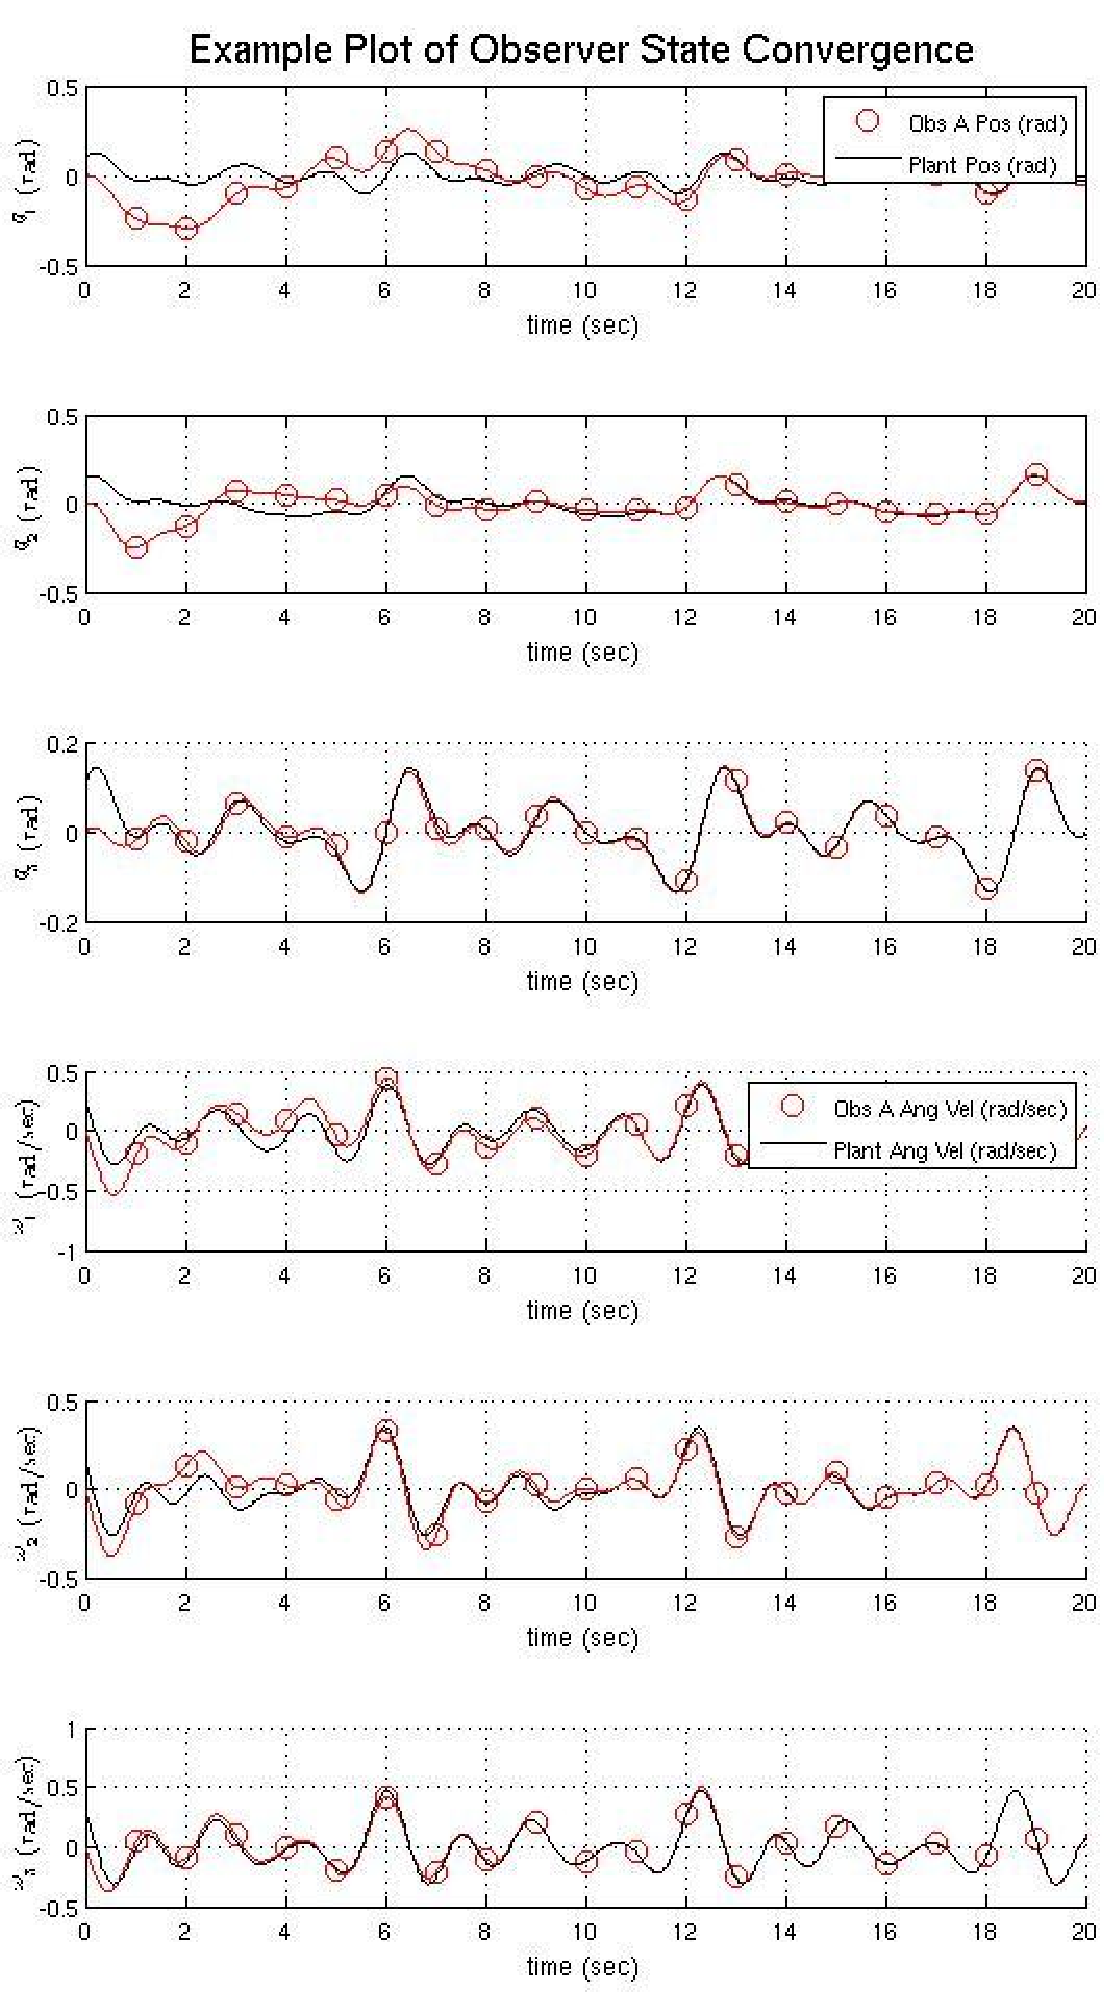
\includegraphics[width=110mm]{./chSMS_ID/images/nextFull3}
    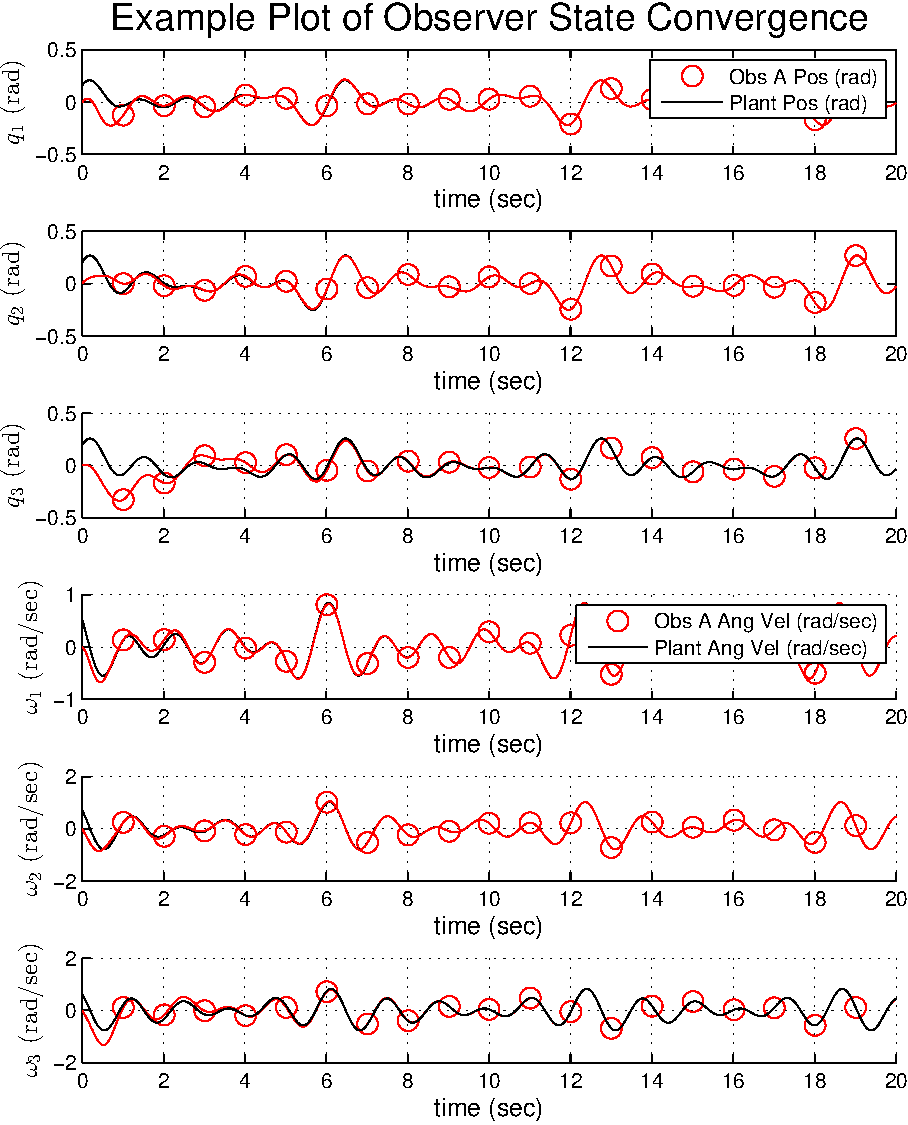
\includegraphics[width=150mm]{./chSMS_ID/images/jhuObsStateConv}
    %{./images/jhuObsFig}
  \end{center}
  \caption{ Angular position and angular velocity simulation the
    plant, (\ref{chModels.eq.SO3plant}), and Observer A,
    (\ref{chSMS_ID.eq.AVO}).  Note convergence of Observer A state to
    plant state in each of the 6 \ac{DOF}.}
  \label{chSMS_ID.fig.AVO}
\end{figure}
\end{center}

This Section reports a comparative analysis of numerical simulations
for the three angular velocity observers described in Sections
\ref{chSMS_ID.sec.AVO}, \ref{chSMS_ID.sec.AVO_Sal}, and
\ref{chSMS_ID.sec.AVO_TT}. We assume the plant's inertia tensor, $I$,
is known and the signals of the plant rotational position, $q(t)$, and
the plant torque input, $\tau(t)$, are available.

Each observer's performance was evaluated numerically using
a fourth order Runge-Kutta numerical solution
with fifth order error control. In every case during simulation
the initial state of the observer was $\hat{q}(0)=\vec{0}$ and
$\hat{\omega}(0)=\vec{0}$. 

Plant position trajectories and control inputs satisfying
(\ref{chModels.eq.SO3plant}) were generated numerically.  Plant position
trajectories, $q(t)$, were generated analytically as a sum of sines
and cosines, each with different frequencies and amplitudes, such that
$\|q(t)\|<\frac{\pi}{2}$.  Corresponding plant velocity signals
$\dot{q}(t)$ and $\omega(t)$ were similarly generated analytically.
Plant signals $\dot{\omega}(t)$ and $\tau(t)$ were computed
numerically. In this simulation study we report
\begin{itemize}
\item the body-frame observer (\ref{chSMS_ID.eq.AVO}) as Observer A, 
\item the world-frame observer (\ref{chSMS_ID.eq.AVO_Sal}) as  Observer B, and
\item the coordinate free observer (\ref{chSMS_ID.eq.AVO_TT}) as Observer C.
\end{itemize}

Feedback gains appearing in the three observers differ in form and
dimension.  In an effort to achieve a fair comparison, we chose
observer gains such that, when the observer error systems were
linearized about the equilibrium point $\Delta q=\Delta \bar{q}=\Delta
\tilde{q}=\vec{0}$ and $\Delta \omega=\vec{0}$, the resulting
linearized gain terms were approximately equal.  Equality was be
achieved for the linearized error dynamics of Observers A and B.  The
gains of Observer C, which differ in structure from A and B, were set
such that the average of the eigenvalues of the gain matrices of its
linearized error dynamics were equal to the average eigenvalue of the
gain matrices of the linearized error dynamics of both Observers A and
B. Given $k\in\mathcal{R}$ such that $k>0$ then each observer was
proven to be locally convergent to the plant's state and the gain
equivalence described was achieved by using the following formulas
%
\vspace{5mm}
\begin{itemize}
\item $E=(\frac{k}{2})I^{-1}$ Observer A
\item $k_p=1$ and $k_v=k$ Observer B
\item $\alpha=\frac{k}{4}g_{avg}$ and $\beta=\frac{1}{2}g_{avg}$ for
   Observer C
\end{itemize}
%
where $g_{avg}$ is the average of the eigenvalues of $I^{-1}$.

To evaluate and compare differences in observer convergence we
simulated a number of scenarios.  For observer gains such that $k>0$,
all three observers were seen to be asymptotically stable (i.e. state
estimates converged to the state of the plant).  For example Figure
\ref{chSMS_ID.fig.AVO} shows a typical case of Observer A converging
to the plant's state in all six \ac{DOF}. Figure
\ref{chSMS_ID.fig.AVO_allNorm} is a sample plot showing the magnitude
of angular position error and angular velocity error with respect to
time for all three observers.  For simulations of plants with
inertia tensor eigenvalues near or less than 1.0, the three
observers seemed to converge in a similar fashion. However, Figure
\ref{chSMS_ID.fig.AVO_allNorm} shows Observer B displaying
under-damped behavior which slows its convergence.  This behavior
diminished as either the gain is increased or the inertia is lowered.
Figure \ref{chSMS_ID.fig.AVO_avgNorm2} shows the average of 50 trials
with inertia tensor eigenvalues less than unity and, on average, you
can see the similar behavior of the different velocity
observers.

\begin{center}
\begin{figure*}[htbp]  
  \begin{center}
    %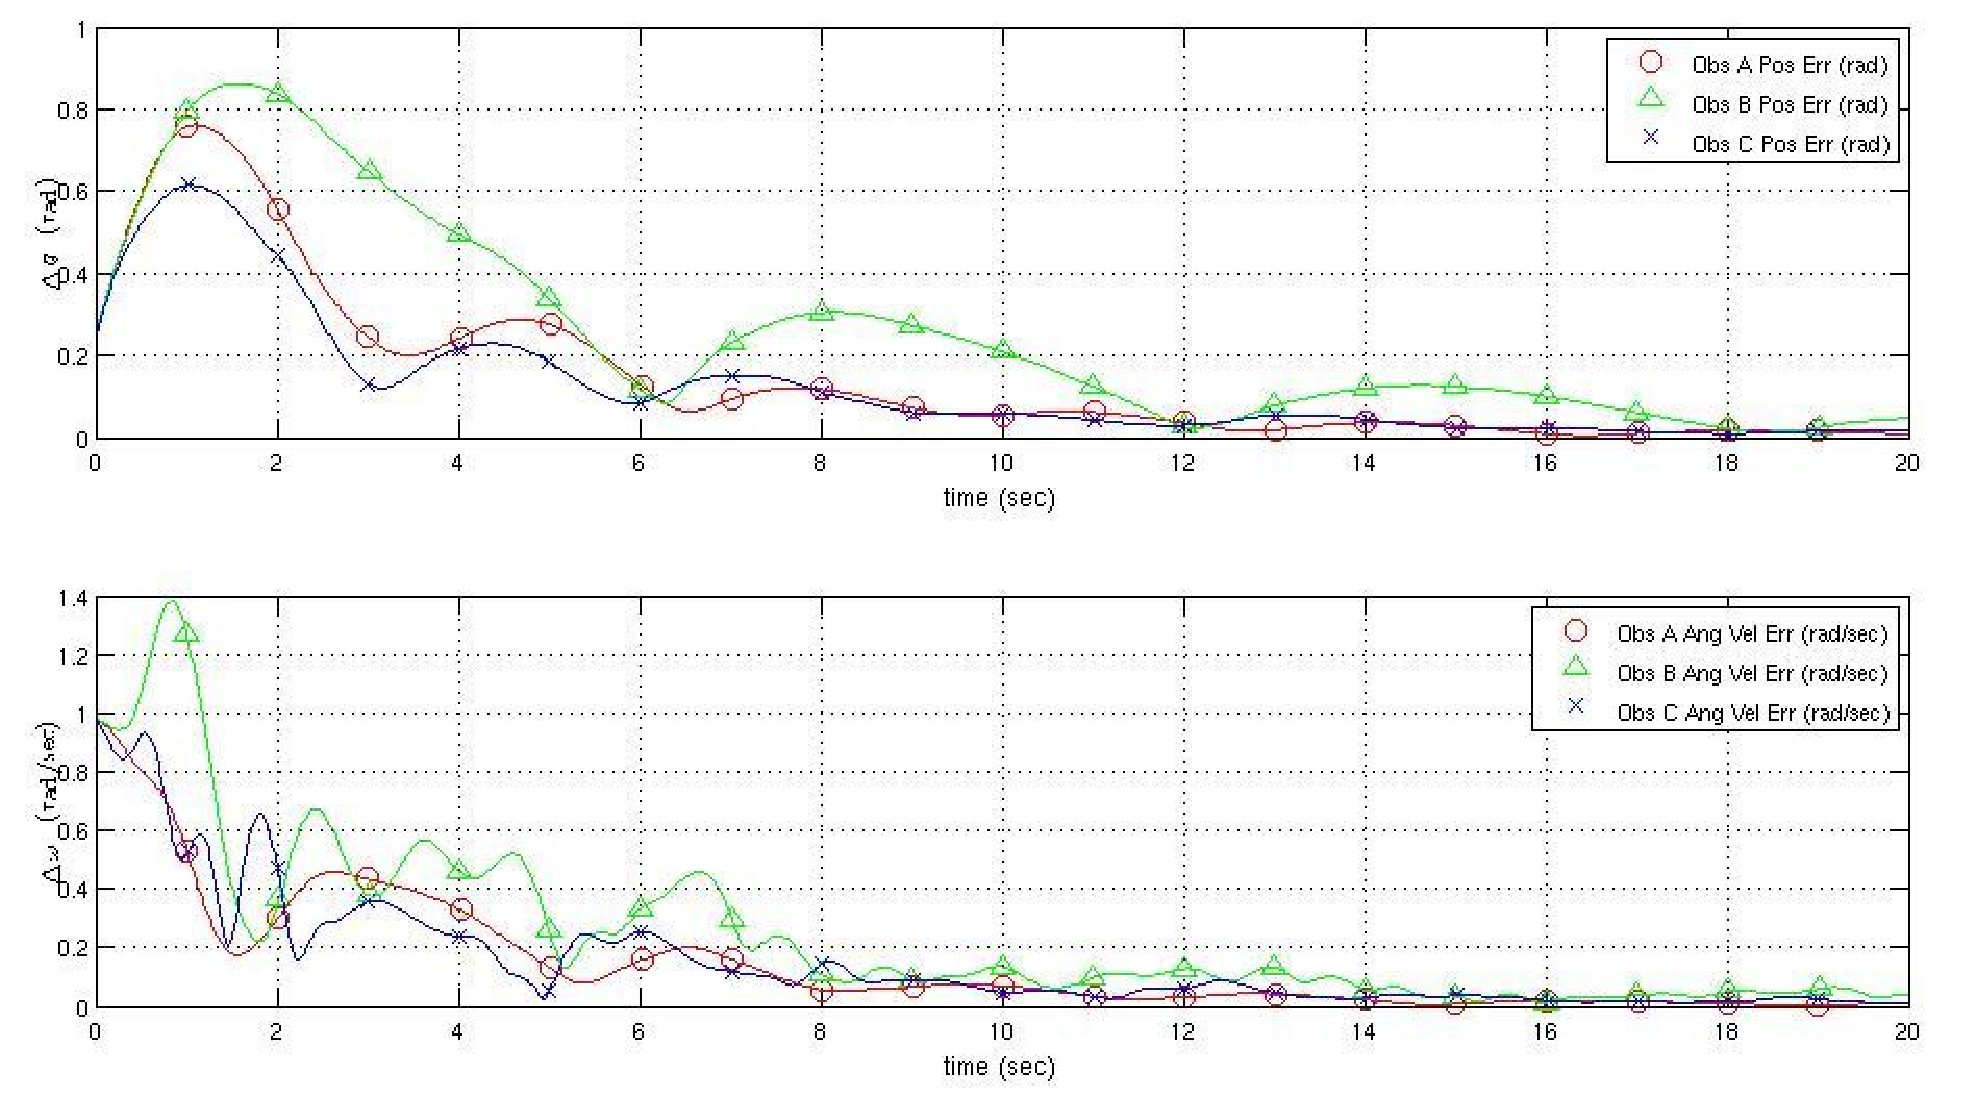
\includegraphics[width=150mm]{./chSMS_ID/images/nextExErr2}%{./images/allNormFig}
    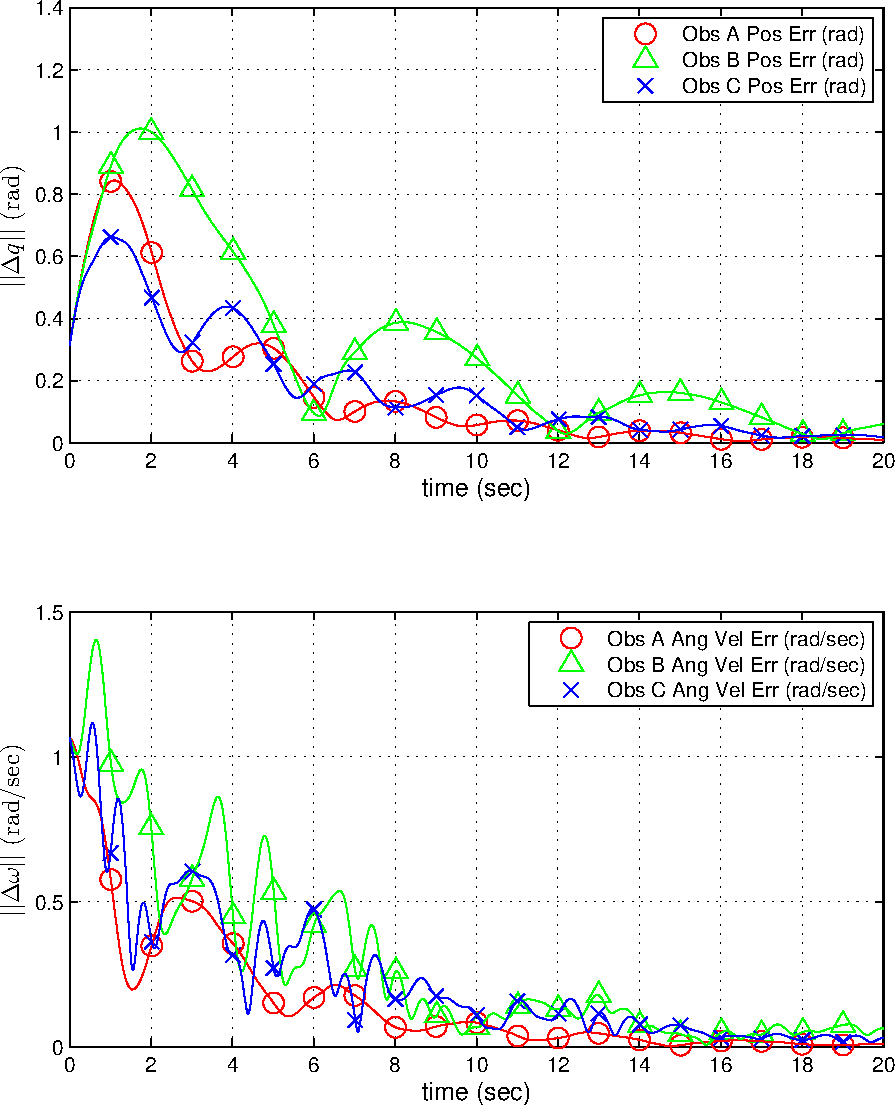
\includegraphics[width=150mm]{./chSMS_ID/images/obsNormErrPlot}%{./images/allNormFig}
  \end{center}
  \caption{Rotational error magnitude and angular velocity error
    magnitude between observer state and plant state.}
  \label{chSMS_ID.fig.AVO_allNorm}
\end{figure*}
\end{center}

\begin{center}
\begin{figure*}[htbp]
  \begin{center}
%    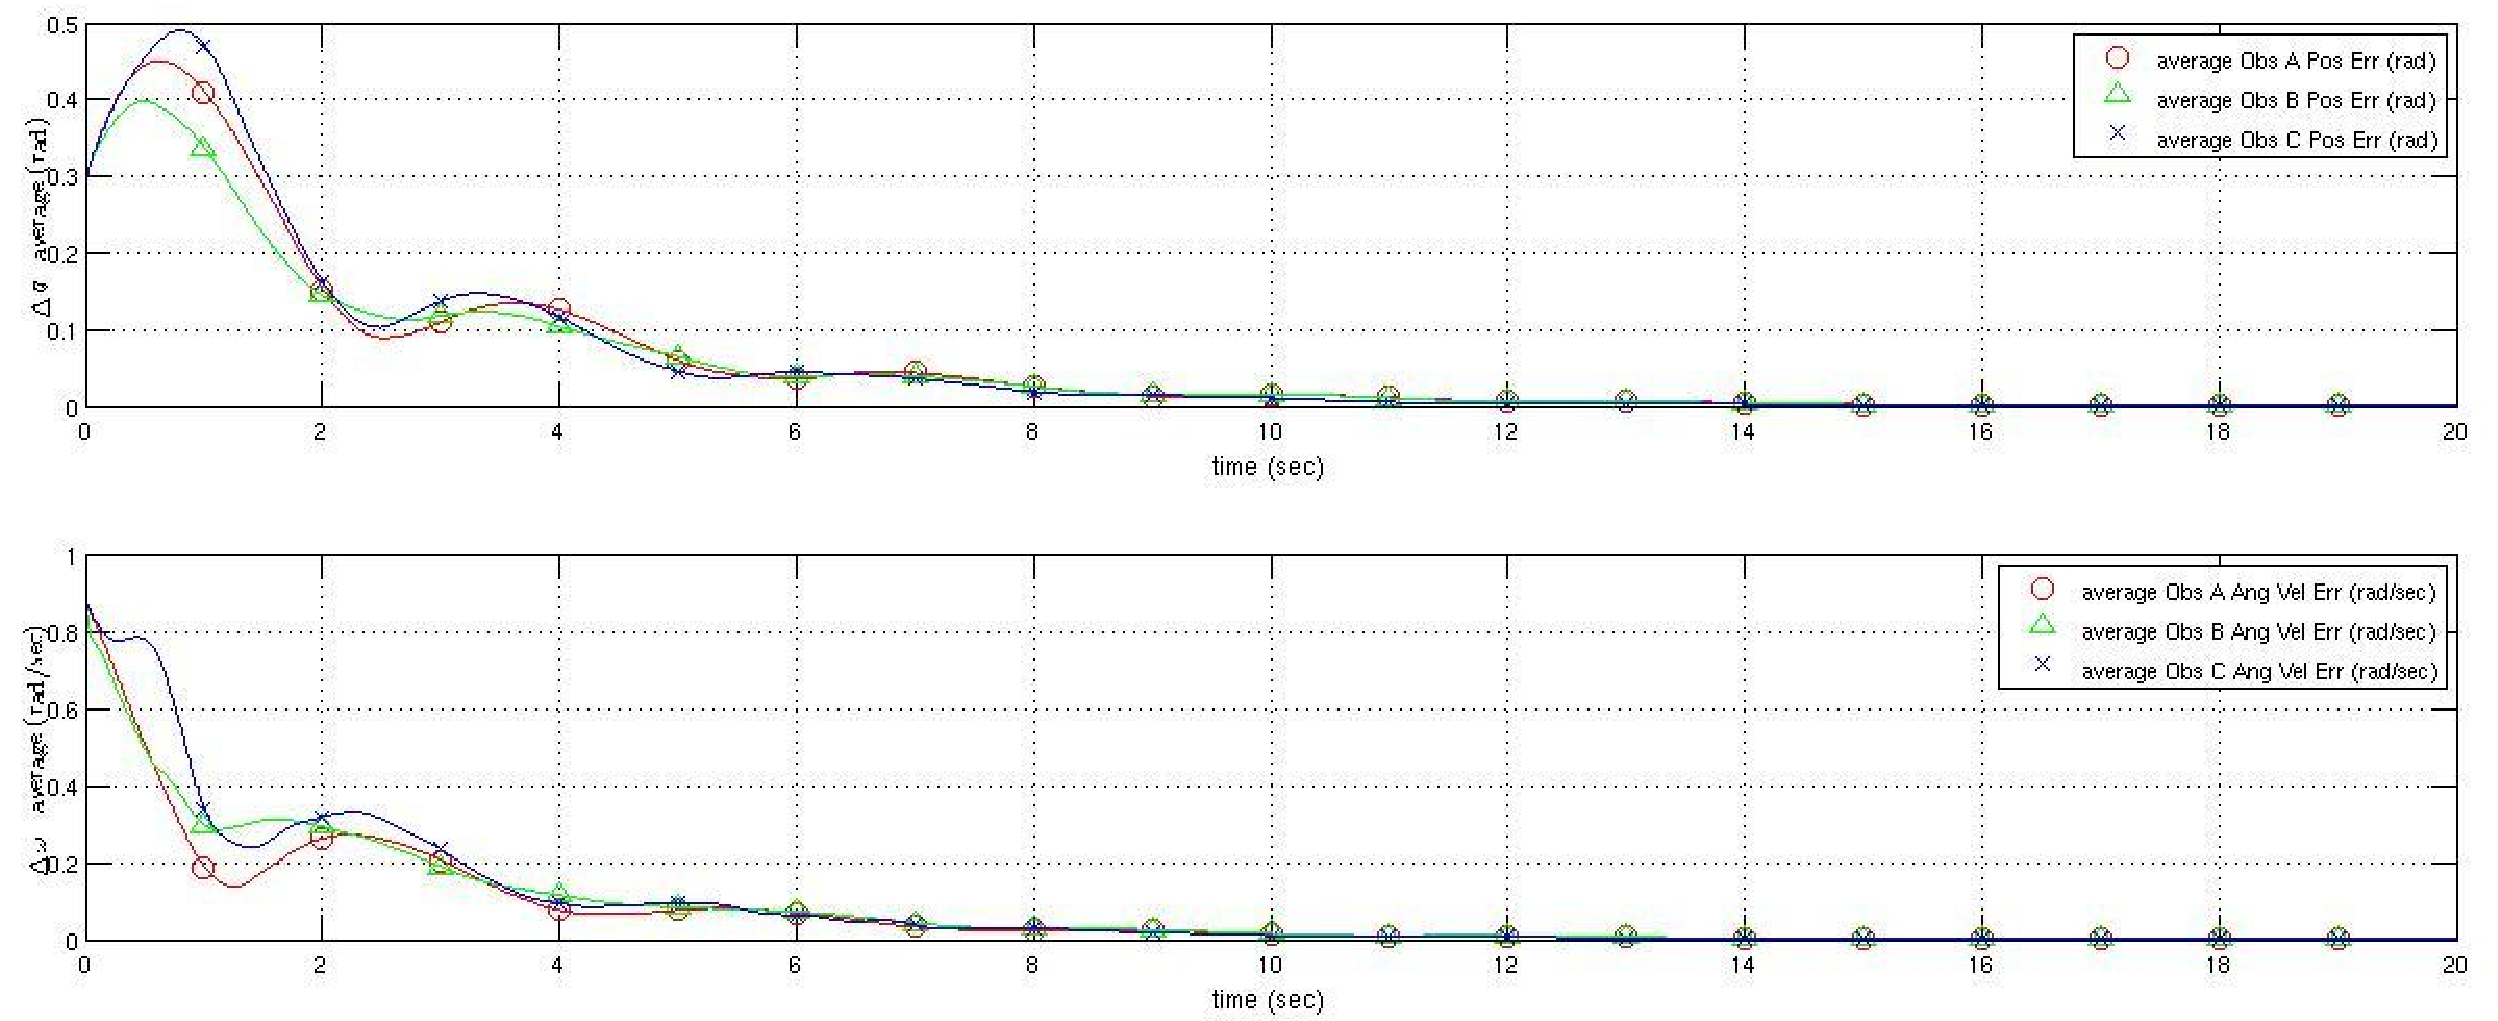
\includegraphics[width=150mm]{./chSMS_ID/images/nextAvgErr2}
    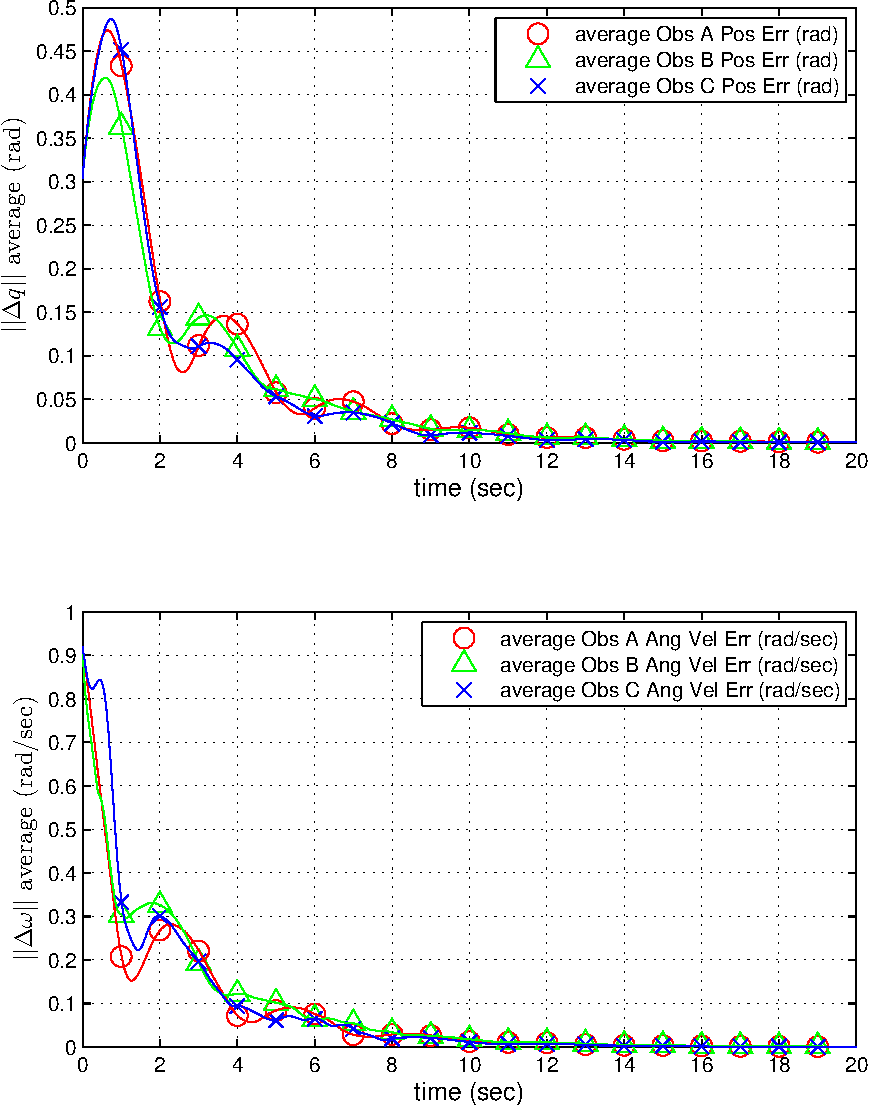
\includegraphics[width=150mm]{./chSMS_ID/images/allObsAvgErr}
  \end{center}
  \caption{Average rotational error magnitude and average angular
    velocity error magnitude between observer state and plant state of
    an ensemble of 50 randomized angular position profile trials and
    inertia tensor eigenvalues less than one.}
  \label{chSMS_ID.fig.AVO_avgNorm2}
\end{figure*}
\end{center}




\subsection{Angular Velocity Observer Conclusions}  
\label{chSMS_ID.sec.AVO_conc}


This Section reports a comparative analysis of three angular velocity
observers for second-order rotational plants of the form
(\ref{chModels.eq.SO3plant}) for which the inertia tensor is known,
and the signals of angular position and torque input are available.
Two very different previously reports angular velocity observers were
reviewed \cite{Salcudean1991,Maithripala2004}.  We report one novel
angular velocity observer together with a proof of its local
asymptotic stability.  The results of a comparative numerical
simulation study of the three observers is reported.  The observers
were seen to provide similar performance over a range of inertia
tensors, angular position profiles, and feedback gains.  For the range
of inertia tensors used, each of the three observers were analytically
guaranteed to converge to the correct angular velocity estimate.
%
However, these analytic stability analyses do not provide information
on the rate of convergence.
%
Each simulated observer's angular velocity estimate converged to the
plant state as expected; however, the coordinate free and body-frame
observers (though more complex to implement) were not seen to display
the underdamped behavior which appeared to degrade the world-frame
observer's state estimate convergence rate for some of the simulated
comparisons in our ensemble of simulation studies.
%
For simple second-order linear systems, underdamped behavior results
from a poorly tuned combination of the proportional and derivative
gains; we would expect similar performance for each of the three
observers when state errors are small enough that the linearization
assumptions used to match the gains are valid.
%Since the structure of this
%nonlinear observer prevents tuning both the proportional and
%derivative gains, 
%
The lack of underdamped behavior in the coordinate free and body-frame
observers could indicate that the additional nonlinear terms improve
performance of both when the linearization assumptions are no longer
valid.
%
However, the difference in structure of these three nonlinear
observers makes it difficult to analytically prove the existence of
such benefits.
%
Exploring these differences, as well as any link between the extra
coordinate free and body-frame terms, is a topic for further research.

\section{ Adaptive Identification for 3-\acs{DOF} Rotational Plants 
  }\label{chSMS_ID.sec.SO3_AID}

This Section addresses the problem of estimation the inertia tensor
of 3-\ac{DOF} rotational plants of the form
(\ref{chModels.eq.SO3plant}).
%
We report a novel \ac{AID} algorithm which estimates the inertia
tensor for a rotating rigid-body using the signals of external torque
and angular velocity.
%
A local stability proof of the new \ac{AID} algorithm is reported.
% 
A numerical simulation study investigates the effect of richness of
the torque input signal on parameter estimation, the effect of
feedback gains, the effect of initial condition, and the domain of
stability.
%
The simulation studies corroborate the analytic stability analysis,
showing that the angular velocity estimate converges asymptotically to
the actual angular velocity of the plant and the adaptive estimate of
the inertia tensor converges to a constant value.
%
Additionally, the simulation studies show that the inertia tensor
estimate converges to the true plant inertia tensor value in the
presence of a sufficiently rich input torque signal.
%
The simulation studies reveal the actual domain of attraction to
exceed the conservative bounds arising in the stability proof, and
identify practically useful ranges of feedback gains.


\subsection{3-\acs{DOF} Rotational Dynamics \acs{AID}} 
\label{chSMS_ID.sec.SO3_AID_Der}

\newcommand{\genericChar}{\psi}
 
Consider a rotating rigid-body under the influence of an
external torque of the form (\ref{chModels.eq.SO3plant}) where the
plant's input torque $\tau(t)$, angular position $R(t)$, and angular
velocity $\omega(t)$ are accessible signals and the plant's \ac{SPD}
inertia tensor is assumed constant but is unknown.
%
We consider the class of inputs $\tau(t)$ such that both
$\tau(t)$ and the angular velocity of the uncontrolled plant,
$\omega(t)$, are bounded.
%
Throughout this Section we will use the following error signals
%
\begin{align}
\Delta\omega(t)&=\hat{\omega}(t)-\omega(t)  \label{chSMS_ID.eq.SO3_AID_deltaw} \\
\Delta I(t)&=\hat{I}(t) - I.                \label{chSMS_ID.eq.SO3_AID_deltaI} 
\end{align}
%
In this Section we will omit explicit notation of variable
dependence on time except where such dependence is required to discuss
the initial condition of the \ac{AID} algorithm.
%



\begin{SO3_AID}
\label{chSMS_ID.theo.SO3_AID}
Consider the following \ac{AID} algorithm for plants of the form
(\ref{chModels.eq.SO3plant})
%
\begin{align}
  \dot{\hat{\omega}}&=\hat{I}^{-1} \mathcal{J}(\hat{I}\omega)\omega
  - a \Delta \omega + \hat{I}^{-1} \tau   \label{chSMS_ID.eq.SO3_AID_estimator}\\
  \dot{\hat{I}}&=-\frac{1}{2}\left(\genericChar_1 \omega^T +\omega \genericChar_1^T
    -\Delta\omega \genericChar_2^T-\genericChar_2 \Delta\omega^T\right)
  \label{chSMS_ID.eq.SO3_AID_identifier}
\end{align}
%
where $a\in\mathbb{R}_+$,  $\genericChar_1=\mathcal{J}(\omega)\Delta \omega$, and 
  $\genericChar_2=\hat{I}^{-1}\left(\mathcal{J}\left(\hat{I}\omega\right)
    \omega +\tau\right)$
with the following assumptions:
%
\begin{itemize}
\item $\tau(t)$ and $\omega(t)$ are bounded
\item $\hat{I}(t_0)$ is \ac{SPD}
\item $\hat{\omega}(t_0)=\omega(t_0)$
\item $\exists \epsilon \in \mathbb{R}_+$ such that $\|\Delta
  I(t_0)\|_F+\epsilon \leq \lambda_3$
\end{itemize}
%
Under these conditions $\lim_{t\to \infty}\Delta \omega=\vec{0}$,
i.e. the estimated angular velocity is asymptotically stable in the
sense of Lyapunov, and $\lim_{t\to \infty}\Delta
\dot{I}=0_{3\times3}$, i.e. the estimated inertia tensor will converge
to a constant value. These limits imply that the plant estimate
converges to values that provide input/output behavior identical to
that of the actual experimental plant for the given input torque
$\tau(t)$.
\end{SO3_AID}

Note that since the initial parameter estimate is \ac{SPD} and the
parameter estimate law is symmetric, both $\hat{I}(t)$ and $\Delta
I(t)$ will be symmetric $\forall t>t_0$, and thus will have strictly
real eigenvalues.


\subsection{Error System}\label{chSMS_ID.sec.SO3_AID_error}

The time derivative of (\ref{chSMS_ID.eq.SO3_AID_deltaI}) is 
%
\begin{align}\label{chSMS_ID.eq.SO3_AID_deltaIdot}
\dot{\Delta I}&=\dot{\hat{I}} \nonumber \\
              &=-\frac{1}{2}\left(\genericChar_1 \omega^T +\omega \genericChar_1^T 
               -\Delta\omega \genericChar_2^T-\genericChar_2 \Delta\omega^T\right).
\end{align}
%
We make use of the fact that $I \hat{I}^{-1}=
\mathbb{I} - \Delta I \hat{I}^{-1}$, where $\mathbb{I}$ is the identity
matrix, thus, 
%
 \begin{align}\label{chSMS_ID.eq.SO3_AID_Ideltawdot}
I\dot{\Delta \omega}
 =&I\left(\dot{\hat{\omega}} - \dot{\omega}\right)
\nonumber \\
 =&-a I \Delta \omega+I \hat{I}^{-1}\mathcal{J}(\hat{I}\omega)\omega
   +I\hat{I}^{-1} \tau-\mathcal{J}(I\omega)\omega-\tau  
\nonumber \\
 =&-a I \Delta\omega+\left(\mathbb{I}-\Delta I\hat{I}^{-1}\right)
    \mathcal{J}(\hat{I}\omega)\omega-\mathcal{J}(I\omega)\omega
   -\Delta I \hat{I}^{-1} \tau
\nonumber \\
 =&-a I \Delta\omega-\mathcal{J}(\omega)\Delta I \omega 
   -\Delta I\hat{I}^{-1}\left(\mathcal{J}(\hat{I}\omega)\omega+\tau\right)
\nonumber \\
 =&-a I \Delta\omega-\mathcal{J}(\omega)\Delta I \omega
   -\Delta I \genericChar_2.
\end{align}


\subsection{Stability Proof}\label{chSMS_ID.sec.SO3_AID_proof}

Consider the following Lyapunov function candidate
%
\begin{equation}\label{chSMS_ID.eq.SO3_AID_lyap}
V(t)=\frac{1}{2}\left(\Delta \omega^{T} I \Delta \omega + 
     \tr\left(\Delta I \Delta I^{T}\right)\right).
\end{equation}
%
$V(t)$ is 
%
positive definite and equal to zero if and only if $\Delta
\omega=\vec{0}$ and $\Delta I=0_{3\times 3}$.
%
%\begin{itemize}
%\item 
%%\item radially unbounded
%\item equal to zero if and only if $\Delta \omega=\vec{0}$ and
%$\Delta I=0_{3\times 3}$.
%\end{itemize}
%
From (\ref{chSMS_ID.eq.SO3_AID_Ideltawdot}) and the fact that for any
matrices $A$ and $B$ of appropriate dimension, $\tr(AB)=\tr(BA)$,
the time derivative of (\ref{chSMS_ID.eq.SO3_AID_lyap}) is
%
\begin{align}
\dot{V}(t) 
 =&\frac{1}{2}\left(\dot{\Delta \omega}^{T} I\Delta\omega
   +\Delta \omega^{T} I \dot{\Delta \omega}
  +\tr\left(2\Delta I \dot{\Delta I}^{T}\right)\right)
  \nonumber  \\
 =&-a\Delta\omega^TI\Delta\omega+\frac{1}{2}\left(\omega^T\Delta I
   \mathcal{J}(\omega)\Delta \omega\right)
   + \tr\left(\Delta I \dot{\Delta I}^T\right)  
  \nonumber  \\
  &+\frac{1}{2}\left(-\genericChar_2^T\Delta I\Delta\omega
  -\Delta \omega^T\mathcal{J}(\omega)\Delta I \omega
  -\Delta \omega^T\Delta I \genericChar_2 \right)
  \nonumber  \\
 =&-a\Delta\omega^TI\Delta\omega+\tr\left(\Delta I \dot{\Delta I}^T\right)
%\nonumber \\
  +\frac{1}{2}\left(
   \omega^T\Delta I\genericChar_1+\genericChar_1^T\Delta I\omega   
   -\genericChar_2^T\Delta I\Delta\omega-\Delta \omega^T\Delta I \genericChar_2\right)
  \nonumber  \\ 
 =&-a\Delta\omega^TI\Delta\omega+\tr\left(\Delta I \dot{\Delta I}^T\right)
% \nonumber \\  
  +\frac{1}{2}\tr\left(
   \Delta I\left(\genericChar_1\omega^T+\omega\genericChar_1^T   
   -\Delta\omega\genericChar_2^T-\genericChar_2\Delta \omega^T\right)\right). 
\end{align}


Using the update law (\ref{chSMS_ID.eq.SO3_AID_identifier}) results in
%
\begin{equation}\label{chSMS_ID.eq.SO3_AID_lyapDot}
\dot{V}(t)=-a\Delta\omega^{T}I\Delta\omega,
\end{equation}
%
which is negative definite in $\Delta \omega$ and negative
semidefinite in the error coordinates $\Delta \omega$ and $\Delta I$.
Lyapunov's theorem and (\ref{chSMS_ID.eq.SO3_AID_lyap}) -
(\ref{chSMS_ID.eq.SO3_AID_lyapDot}) imply that $\Delta \omega$ and
$\Delta I$ are bounded and stable.  The structure of $\dot{V}(t)$
implies that $\Delta \omega \in \mathcal{L}_2$ or, equivalently,
$\lim_{t\to\infty}\left( \int_0^t\Delta \omega^T \Delta
  \omega\right)^{1/2}<\infty$.  To ensure all the signals in
(\ref{chSMS_ID.eq.SO3_AID_estimator}) are bounded, we must ensure that
both $\hat{I}(t)$ and $\hat{I}^{-1}(t)$ remain bounded. The facts $0
\leq V(t) \leq V(t_0)$, $\Delta \omega(t_0)=\vec{0}$, $ \Delta \omega
^T(t) I \Delta \omega (t)\geq 0$ for all $t$, and $\tr\left(\Delta
  I(t) \Delta I^T(t)\right)=
\sum_{i=1}^3|\Delta\lambda_i(t)|^2=\|\Delta I(t)\|_F^2$ imply that the
following inequality holds for all time:
%
\begin{equation}
\|\Delta I(t)\|_F\leq \|\Delta I(t_o)\|_F.
\end{equation}
%
By the Rayleigh-Ritz Theorem, $\min_{\|x\|=1} x^T \hat{I}(t)
x=\hat{\lambda}_3(t)$.  Additionally since $\hat{I}(t)=I+\Delta I(t)$
and by assumption $\|\Delta I(t_0)\|_F+\epsilon\leq\lambda_3$ the
following inequalities hold
%
\begin{align}
\hat{\lambda}_3(t)
 &= \min_{\|x\|=1}\left(x^T I x + x^T \Delta I(t) x\right)
\nonumber \\
 &\geq\min_{\|x\|=1}\left(x^T I x\right)-\max_{\|x\|=1}|x^T\Delta I(t)x|
\nonumber \\
 &\geq\lambda_3-\|\Delta I(t)\|_2
\nonumber \\
 &\geq\lambda_3-\left(\sum_{i=1}^3|\Delta\lambda_i(t)|^2\right)^{1/2}
\nonumber \\
 &\geq\lambda_3-\|\Delta I(t)\|_F
\nonumber \\
 &\geq\lambda_3-\|\Delta I(t_0)\|_F
\nonumber \\
 &\geq\lambda_3-\left(\lambda_3-\epsilon\right)
\nonumber \\
 &\geq\epsilon
\end{align}
%
\sloppy{ \noindent where $\epsilon$ is a finite positive scalar and we use the fact that
$\|\Delta I(t)\|_2^2=\max(|\Delta \lambda_1(t)|^2,|\Delta \lambda_3(t)|^2)$
because the singular values of a symmetric matrix are equal to the
absolute values of its eigenvalues.  The above inequality guarantees
that all eigenvalues of $\hat{I}(t)$ are positive and bounded away
from zero for all time.  Similarly,}
%
\begin{align}
\hat{\lambda}_1(t)
 &= \max_{\|x\|=1}\left(x^T I x + x^T \Delta I(t) x\right)
\nonumber \\
 &\leq \lambda_1 +\max_{\|x\|=1}|\left(x^T \Delta I(t) x\right)|
\nonumber \\
  &\leq \lambda_1 +\left(\sum_{i=1}^3|\Delta\lambda_i(t)|^2\right)^{1/2}
\nonumber \\
  &\leq \lambda_1 +\lambda_3 -\epsilon
\end{align}
%
which implies that the eigenvalues of $\hat{I}(t)$ are
positive and bounded above for all time since $\epsilon<\lambda_3$. Since the 
input $\tau$ and plant state $\omega$ are bounded by assumption,
bounded $\Delta \omega$, $\hat{I}$, and $\hat{I}^{-1}$ imply that
$\dot{\omega}$ and $\dot{\hat{\omega}}$ are bounded.  The bounded
angular velocities imply $\Delta \dot{\omega}$ is bounded.  Note that
bounded $\Delta \dot{\omega}$ and $\Delta \omega \in \mathcal{L}_2$
implies
%
\begin{equation}
\lim_{t\to \infty}\Delta\omega=\vec{0}.
\end{equation}
%
Since every signal in $\dot{\hat{I}}$ is bounded and
$\lim_{t\to \infty}\Delta\omega=\vec{0}$ this implies
%
\begin{equation}
\lim_{t\to \infty}\dot{\hat{I}}=0_{3 \times 3}.
\end{equation}
%
Thus, the estimator's angular velocity asymptotically converges to the
angular velocity of the actual plant, and the estimated inertial
tensor, $\hat{I}$, asymptotically converges to a constant value. The
local stability of the \ac{AID} algorithm for 3-\ac{DOF} rotational
plants is proven.

\subsection{Simulation}\label{chSMS_ID.sec.SO3_AID_Sim}

This Section describes the performance of the proposed \ac{AID}
algorithm in numerical simulation.  The numerical results presented
herein used a fourth order Runge-Kutta numerical solution to simulate
both the \ac{AID} algorithm, (\ref{chSMS_ID.eq.SO3_AID_estimator})
and (\ref{chSMS_ID.eq.SO3_AID_identifier}), and the plant,
(\ref{chModels.eq.SO3plant}).  Since the \ac{AID} algorithm assumed
access to both $\omega(t)$ and $\tau(t)$, without loss of generality we
choose $\hat{\omega}(t_0)=\omega(t_0)$. The input torque $\tau(t)$ was
generated as a sum of sines and cosines, each with different
frequencies and amplitudes.  In each trial the plant's inertia tensor,
$I$, was chosen and the inertia tensor estimate was initialized to the
identity matrix, i.e. $\hat{I}(t_0)=\mathbb{I}$.


\subsubsection{Convergence of State and Parameter Estimates}

To test the differences in identification performance we explored the
effects of factors including initial parameter error, input torque
richness, and feedback gain.  Figure \ref{chSMS_ID.fig.SO3_AID_basic} is
representative of simulated performance in the majority of cases.
This representative simulation study used a
feedback gain $a=1$; an input torque of
%
\begin{equation}
\tau(t)=\left[ \begin{array}{ccc}-2\cos(2t)& -2\sin(t)
    &2cos(t)\end{array}\right]^{T};
\end{equation}
%
an inertia tensor of $I=1.5\mathbb{I}$; and an estimate of
$\hat{I}(t_0)=\mathbb{I}$ (this was the initial inertia tensor for
every simulation study in this Section).  This Figure explicitly shows
state and parameter convergence of the angular velocity and inertia
tensor eigenvalue estimates.  The eigenvalues of the \ac{SPD} inertia
tensors are plotted to show parameter convergence.

\begin{center}
\begin{figure}[htbp]
  \begin{center}
    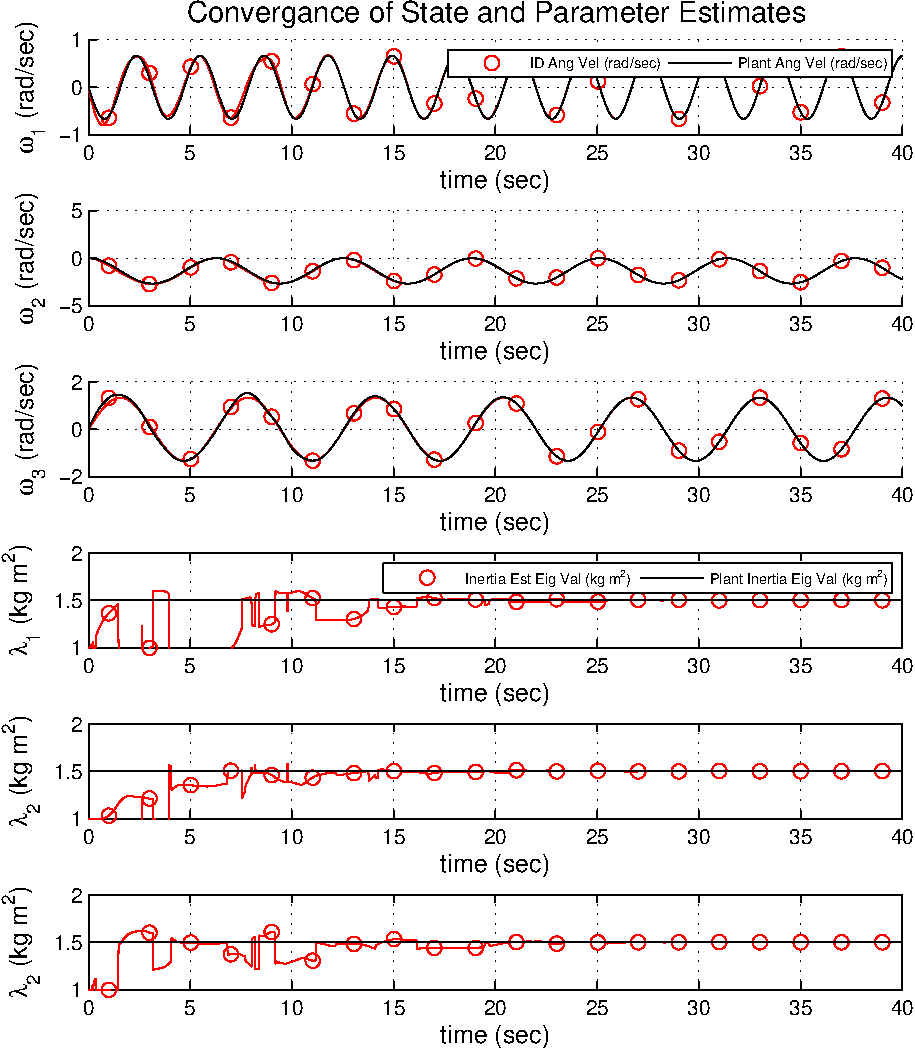
\includegraphics[width=150mm]{./chSMS_ID/images/SO3AID_stateParamConv}
  \end{center}
  \caption{ Data showing state and parameter convergence during a
    representative simulation study.  Estimated values are highlighted
    with circles.  The top three plots show the estimated angular
    velocity's convergence to the true plant angular velocity in each
    \ac{DOF}.  The bottom three plots show the eigenvalues of the
    estimated inertia tensor converging the true inertia tensor
    eigenvalues.}
  \label{chSMS_ID.fig.SO3_AID_basic}
\end{figure}
\end{center}


\subsubsection{Effect of Scalar feedback Gain Parameter $a$}

Figure \ref{chSMS_ID.fig.SO3_AID_gains} shows how \ac{AID} algorithm performance
varies with changes of the scalar gain $a$.  In the case that $a$ is
large, the angular velocity error remains small for all time, and  the
small angular velocity error limits the ability of this error signal
to drive parameter adaptation as seen in
(\ref{chSMS_ID.eq.SO3_AID_identifier}).  For the case of very small
values of $a$, the parameter convergence is slow.  In the limiting
case of $a=0$ the identifier is stable, but not asymptotically stable.

\begin{center}
\begin{figure}[htbp]
  \begin{center}
    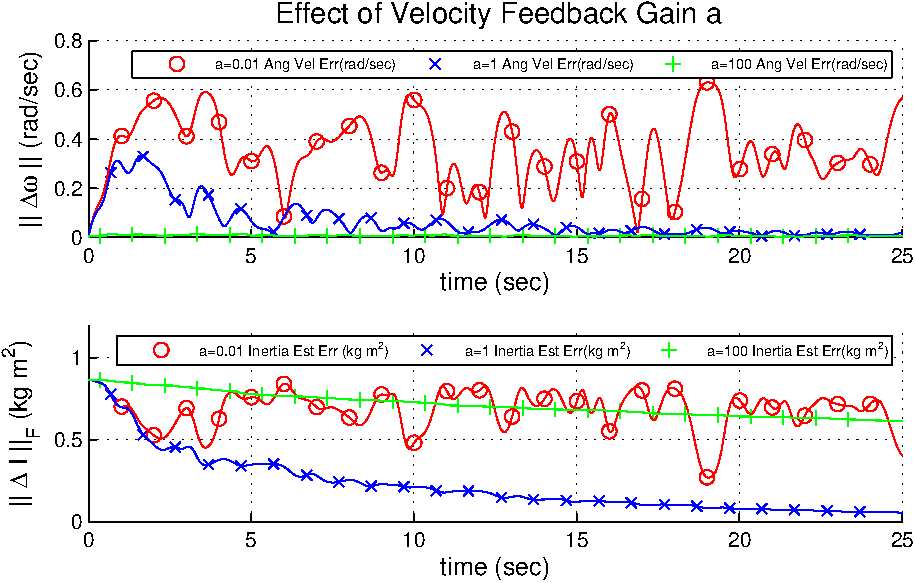
\includegraphics[width=150mm]{./chSMS_ID/images/gainFig01}
  \end{center}
  \caption{The effect of the feedback gain, $a$, on angular velocity and
    parameter convergence.  The upper graph plots the norm of the body
    angular velocity error versus time.  The lower graph plots the
    Frobenius norm of the inertia tensor error versus time.  The cases
    of \ac{AID} for $a=0.01$, $a=1.0$, and $a=100$ are
    shown.  Parameter convergence deteriorates for very large and very
    small gains.  }  \label{chSMS_ID.fig.SO3_AID_gains}
\end{figure}
\end{center}

\subsubsection{Effect of Input $\tau(t)$ Richness}

Figure \ref{chSMS_ID.fig.SO3_AID_perExcit} demonstrates the well know
fact that exact parameter identification requires a sufficiently rich
input torque signal.  For these simulations we employed the following
values for the identification algorithm: $a=1$, $I=1.5\mathbb{I}$,
$\hat{I}(t_0)=\mathbb{I}$, and either
$\tau(t)=\left[\begin{array}{ccc}-2\cos(2t)& -2\sin(t)&
    2\cos(t)\end{array}\right]^{T}$ or
$\tau(t)=\left[\begin{array}{ccc}0& -2\sin(t)&
    0\end{array}\right]^{T}$.  In both cases the estimated angular
velocity converged to the true angular velocity. For the case of the
richer input signal, the inertia tensor estimate converged to the
actual plant inertia tensor value.  
%
For the case of the simple input signal, however, the inertia tensor
estimate converged to a value different from the plant's inertia
tensor value.
%
Note that the inertia tensor estimate still converged to a value that
results in identical input-output behavior of the {\it estimated
  plant} and actual plant for this simple input signal (where an {\it
  estimated plant} is a second-order rotational plant of the form
(\ref{chModels.eq.SO3plant}) with its inertia tensor equal to an
inertia tensor estimate).


 \begin{center}
 \begin{figure}[htbp]
   \begin{center}
     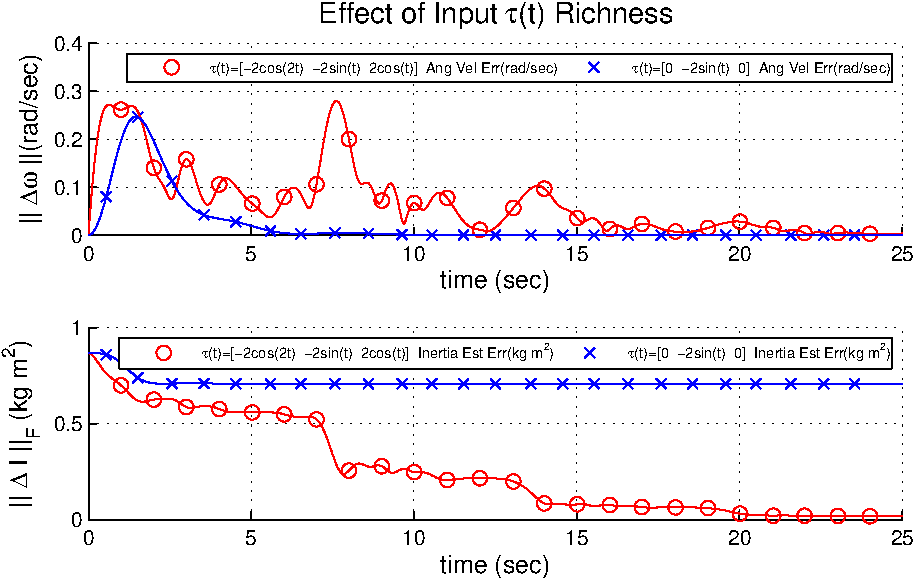
\includegraphics[width=150mm]{./chSMS_ID/images/perExcit01}
   \end{center}
   \caption{ Two plots showing that parameter convergence requires a
     sufficiently rich input signal.  The upper graph plots the norm
     of the body angular velocity error versus time for two inputs
     $\tau(t)$.  The lower graph plots the Frobenius norm of the inertia
     tensor error versus time for both cases.  The angular velocity
     estimate converges in either case. $\tau(t)=[0\quad -2\sin(t)\quad 0]$ is not
     rich enough to force parameter convergence for this initial
     condition, whereas parameter convergence occurs for input torque
     $\tau(t)=[-2\cos(2t)\quad -2\sin(t)\quad 2\cos(t)]$.  }
   \label{chSMS_ID.fig.SO3_AID_perExcit}
 \end{figure}
 \end{center}

\subsubsection{Effect of $\hat{I}(t_0)$}


This Section examines the effect of initial parameter estimate error,
$\Delta I(t_0)$, on parameter convergence. Figure
\ref{chSMS_ID.fig.SO3_AID_smallRange} shows parameter convergence for
30 simulated initial conditions. In all cases
$\hat{I}(t_0)=\mathbb{I}$ and $a=1$. In each case $\tau(t)$ was generated
from sums of sinusoids of different frequencies with randomly
generated amplitudes.  Three sets of ten inertia tensors were used.
Every inertia tensor was randomly generated such that it was a
non-diagonal \ac{SPD} matrix with the eigenvalues greater than
0.5. Within each set the Frobenius norm of $\|\Delta I(t_0)\|_F$ was
either 0.15, 0.5, or 1. Figure \ref{chSMS_ID.fig.SO3_AID_smallRange}
plots parameter convergence of the \ac{AID} algorithm to every
inertia tensor in each of the three sets. For sets one and two, with
$\|\Delta I(t_0)\|_F=0.15$ and $\|\Delta I(t_0)\|_F=0.5$, all
conditions of Theorem \ref{chSMS_ID.theo.SO3_AID} were met. For set
three, often $\|\Delta I(t_0)\|_F>\lambda_3$ and thus the conditions
of Theorem \ref{chSMS_ID.theo.SO3_AID} were not met.  Despite this,
every inertia tensor estimate converged to the true inertia tensor for
each randomly generated initial condition. This convergence
corroborates our analytic result and indicates that the condition
requiring $\|\Delta I(t_0)\|_F<\lambda_3$ from Theorem
\ref{chSMS_ID.theo.SO3_AID} is sufficient but not necessary for
asymptotic convergence.


\begin{center}
\begin{figure}[htbp]
  \begin{center}
    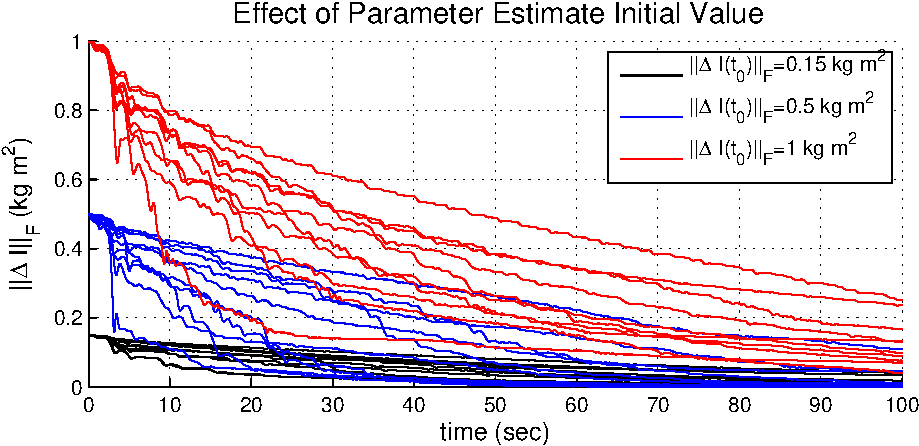
\includegraphics[width=150mm]{./chSMS_ID/images/inertiaEstimateInitErr}
  \end{center}
  \caption{ Three sets of ten simulations showing parameter
    convergence.  The Frobenius norm of the inertia tensor error is
    plotted versus time. Each of the simulations used a randomly
    selected inertia tensor for the system, but within each set the
    Frobenius norm of the initial inertia error was a constant value
    for the entire set, either 0.15, 0.5, or 1.}
  \label{chSMS_ID.fig.SO3_AID_smallRange}
\end{figure}
\end{center}


%\begin{center}
%\begin{figure}[htbp]
%  \begin{center}
%    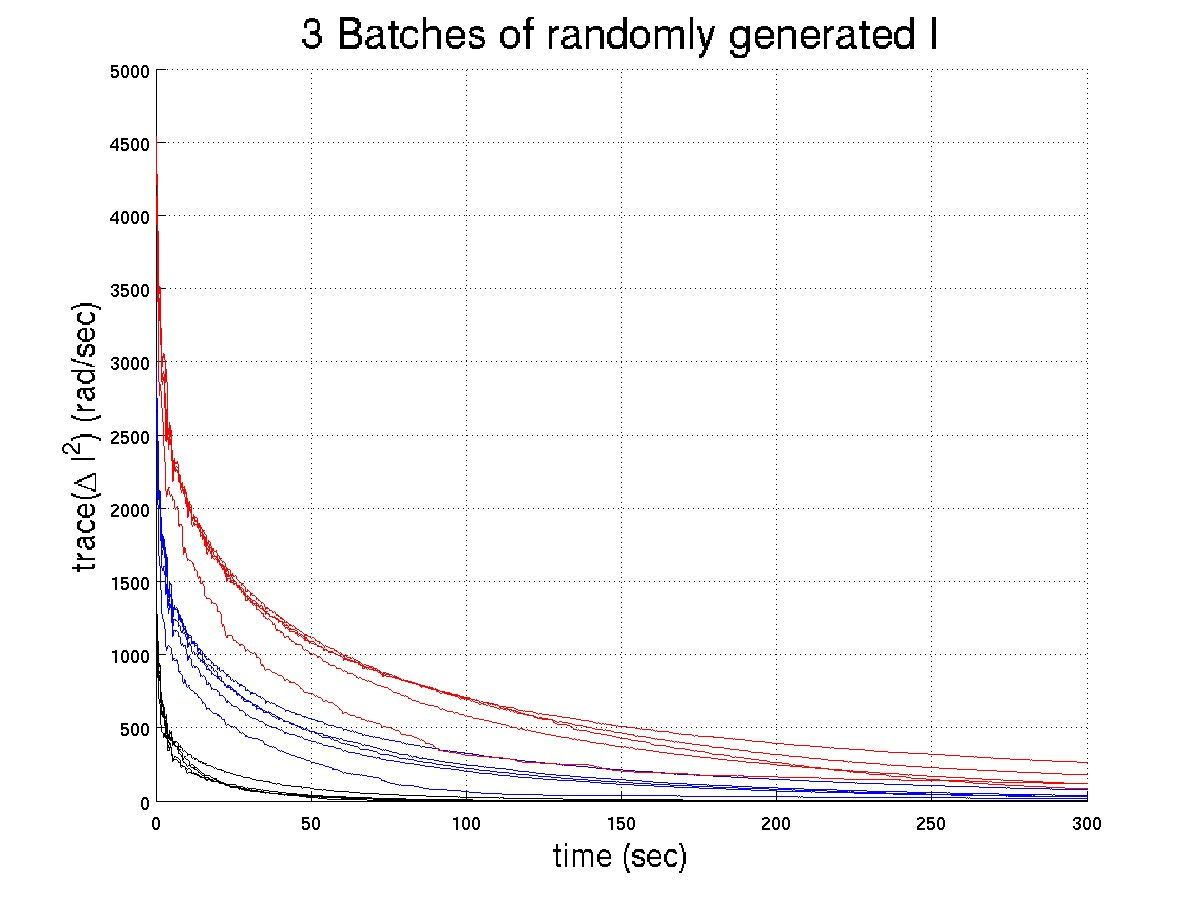
\includegraphics[width=90mm]{./images/largeRangeFig}
%  \end{center}
%  \caption{ 3 sets of 5 simulations of parameter convergence, with
%    each set having a random initialization but a set error between I
%    and $\hat{I}(t_0)$.  Note that for all three set of 5 the
%    parameter error is many orders of magnitude larger than errors
%    which would meet the conditions set forth in Theorem \ref{SO3_ID}.}
%  \label{fig:largeRange}
%\end{figure}
%\end{center}

%One of the most limiting requirements of Theorem \ref{SO3_ID} is the
%requirement for $\hat{I}(t_0)$ to start so close in the neighborhood
%of $I$.  Since both $\hat{I}(t)$ and $\hat{I}(t)^{-1}$ appear in the
%parameter update law, the neighborhood requirement stated in Theorem
%\ref{SO3_ID} was chosen such that Lyapunov Stability would make
%reaching a singularity impossible.  In practice, especially if the
%eigenvalues of the true Moment of Inertia are much larger than the
%Moment of Inertia eigenvalues which the identification algorithm is
%initialized at, our experience is that the neighborhood requirement
%placed on $\hat{I}(t_0)$ is very conservative.   



\subsection{ 3-\acs{DOF} Rotational Plant \acs{AID} Conclusion}

This Section reports an \ac{AID} algorithm for the dynamic estimation
of the inertia tensor of rotating plants.
%
The proof of Theorem \ref{chSMS_ID.theo.SO3_AID} shows the local
asymptotic stability of the estimated angular velocity to the plant's
angular velocity and the local stability of the estimated inertia
tensor. 
%
Numerical simulations show that for a sufficiently rich external
torque signal the inertia tensor estimate value converges to the true
inertia tensor value, and the domain of attraction of Theorem
\ref{chSMS_ID.theo.SO3_AID} is conservative.
%
In Chapter \ref{chUV_AID}, Theorems \ref{chUV_AID.theo.UV_SO3_AID} and
\ref{chUV_AID.theo.UV_SE3_AID} extend this result to plant models of
\ac{UV} dynamics.

\section{Adaptive Identification for Open Kinematic Chains }
\label{chSMS_ID.sec.OKC_AID}

This Section addresses the problem of parameter estimation for an {\it n}-link
\acf{OKC} of the form of (\ref{chModels.eq.OKCplant}). We report a
novel \ac{AID} algorithm  which estimates these plant parameters.
This algorithm assumes the joint torque inputs, $\OKCinput$, joint
positions, $\OKCpos$, and joint velocities, $\dot{\OKCpos}$, are
accessible signals. 


%This Section proves the stability of a previously unreported
%nonlinear adaptive identifier for general \ac{OKC}.



\subsection{\acs{OKC} State Error Coordinates}

The \ac{AID} algorithm presented herein uses the joint velocity
estimate $v\in \mathbb{R}^{n}$ and the parameter vector estimate
$\OKCparamEst\in\mathbb{R}^{r}$ as its state variables. Let
$\mathfrak{J}\subset\rSp{n}$ be the \ac{OKC}'s joint space and note
estimated plant terms $\hat{M}$, $\hat{C}$, and $\hat{\OKCg}$ can be
factored as
%
\begin{equation}
\hat{M}(a)b+\hat{C}(a,c)d+\hat{\OKCg}(a)=\OKCreg(b,a,c,d)\OKCparamEst
\end{equation}
%
for all $a,b,c,d\in\rSp{n}$ where
\funDefn{\OKCreg}{\rSp{n}\times\mathfrak{J}\times\rSp{n}\times\rSp{n}}{\rSp{n\times
    r}} is often termed the {\it regressor}.
%
We employ the following joint velocity and inertia tensor
error coordinates
%
\begin{align}
\Delta v&=v(t)-\dot{\OKCpos}(t)           \label{chSMS_ID.eq.OKC_AID_deltaVel} \\
\Delta \OKCparam&=\OKCparamEst(t) - \OKCparam.    \label{chSMS_ID.eq.OKC_AID_deltaPar} 
\end{align}
%
%Talk about eigenvalue conventions and vector-matrix norms here if
%required 
%
Our goal is to develop an update law for $v$ and
$\OKCparamEst$ which, for initial values of $\OKCparamEst(t_0)$ in the
neighborhood of $\OKCparam$, guarantees that $\lim_{t\to
  \infty}\Delta v=\vec{0}$ and $\lim_{t\to \infty}\Delta
\OKCparamDot=\vec{0}$. Considering torque as the system input and
joint velocity as the system output, the two limits above imply the
input-output behavior of the estimator asymptotically converges to the
input-output behavior of the plant.


\subsection{Adaptive Identifier Description}



\begin{OKC_AID} \label{chSMS_ID.theo.OKC_AID}
  Consider the following \ac{AID} algorithm for plants of the form
  (\ref{chModels.eq.OKCplant}):
%
  \begin{align}
    \dot{v}&=\hat{M}^{-1}(\OKCpos) \left(\OKCinput - \hat{C}(\OKCpos,\dot{\OKCpos}) v
      -\hat{\OKCg}(\OKCpos)- K\Delta v\right)
                                              \label{chSMS_ID.eq.OKC_AID_estimator}\\
    \OKCparamEstDot&= \OKCreg(\dot{v},\OKCpos,\dot{\OKCpos},v)^T\Delta v,
                                              \label{chSMS_ID.eq.OKC_AID_identifier}
  \end{align}
%
  where $K\in\rSp{n\times n}$ is \ac{SPD}, with the following assumptions:
%
  \begin{itemize}
  \item $\OKCinput$, $\OKCpos$ and $\dot{\OKCpos}$ are bounded by assumption
  \item $v(t_0)=\dot{\OKCpos}(t_0)$
  \item $\exists \epsilon \in \rSp{}_+$ such that
% 
    \begin{equation}
      \label{chSMS_ID.eq.OKC_AID_massLowerBound}
      \|\Delta
      \OKCparam(t_0)\|_2\leq \frac{1}{\sqrt{a_M r}}\left(\lambda_m-\epsilon\right)
    \end{equation}
%
    where $\lambda_m$ is the smallest eigenvalue for $M(\OKCpos)$ in
    any configuration and 
%
\begin{equation}
  a_M=\max_{\hat{\theta}\in\{e_1,e_2,...,e_r\}}\left(\max_{\OKCpos\in\rSp{r}}\left(\eig(\hat{M}(\OKCpos))\right)\right)
\end{equation}
%
where the set $\{e_i\}$ are the standard unit length basis vectors of the space $\rSp{r}$
%$a_M=$ is the largest eigenvalue of
%    $\hat{M}(\OKCpos)$ for any configuration corresponding to
%    $\OKCparamEst=e_i$ for all the standard unit length basis vectors
%    $e_i$ 
(see Section \ref{chSMS_ID.sec.OKC_AID_boundM} for a
    complete development of $a_M$).
  \end{itemize}
%
  \noindent Under these conditions the joint velocity error will
  be asymptotically stable in the sense of Lyapunov, i.e., $\lim_{t\to
    \infty}\Delta v =\vec{0}$, and the model using the estimated
  parameters will be indistinguishable from the model using the true
  parameters for the given torque input, i.e., $\lim_{t\to
    \infty}\Delta \OKCparamDot=0$.
\end{OKC_AID}

\subsection{Error System}\label{chSMS_ID.sec.OKC_AID_error}

Consider (\ref{chModels.eq.OKCplant}),
(\ref{chSMS_ID.eq.OKC_AID_estimator}), (\ref{chModels.eq.OKCplantW}),
and (\ref{chSMS_ID.eq.OKC_AID_deltaPar}) as well as the fact that
%
\begin{equation*}
\left(\OKCreg(b_1,a,c,d_1)-\OKCreg(b_2,a,c,d_2)\right)\OKCparam=M(a)(b_1-b_2)+C(a,c)(d_1-d_2)
\end{equation*}
%
in the following equalities
%
\begin{align}
  0&=\OKCinput-\OKCinput  \nonumber \\
  &=\OKCreg(\dot{v},\OKCpos,\dot{\OKCpos},v)\OKCparamEst
  + K\Delta v - \OKCreg(\ddot{\OKCpos},\OKCpos,\dot{\OKCpos},\dot{\OKCpos})\OKCparam \nonumber \\
  &=\OKCreg(\dot{v},\OKCpos,\dot{\OKCpos},v)\Delta\OKCparam + K\Delta v+\left(
    \OKCreg(\dot{v},\OKCpos,\dot{\OKCpos},v)
    - \OKCreg(\ddot{\OKCpos},\OKCpos,\dot{\OKCpos},\dot{\OKCpos})\right)\OKCparam     \nonumber \\
  &=\OKCreg(\dot{v},\OKCpos,\dot{\OKCpos},v)\Delta\OKCparam + K\Delta v +
  M(\OKCpos)\Delta \dot{v}+C(\OKCpos,\dot{\OKCpos})\Delta v. 
  \label{chSMS_ID.eq.OKC_torqueTrick}
\end{align} 
%
The final equality of (\ref{chSMS_ID.eq.OKC_torqueTrick}) can be
rewritten as
%
\begin{equation}\label{chSMS_ID.eq.OKC_AID_deltaJointAcc}
\Delta\dot{v}=M^{-1}(\OKCpos)\left(-C(\OKCpos,\dot{\OKCpos})\Delta v 
   -K\Delta v-\OKCreg(\dot{v},\OKCpos,\dot{\OKCpos},v)\Delta \OKCparam\right).
\end{equation}

\subsection{Lyapunov Stability}\label{chSMS_ID.sec.OKC_AID_lyap}

Consider the following Lyapunov function candidate:
%
\begin{equation}\label{chSMS_ID.eq.OKC_AID_lyap}
V(t)=\frac{1}{2}\Delta v^{T} M(\OKCpos) \Delta v + 
     \frac{1}{2}\Delta \OKCparam^{T} \Delta \OKCparam.
\end{equation}
%
$V(t)$ is
%
\begin{itemize}
\item positive definite
\item radially unbounded
\item equal to zero if and only if $\Delta v=\vec{0}$ and
$\Delta \OKCparam=\vec{0}$.
\end{itemize}
%
Using (\ref{chSMS_ID.eq.OKC_AID_deltaJointAcc}) the time derivative of
(\ref{chSMS_ID.eq.OKC_AID_lyap}) is
%
\begin{align*}
\dot{V}(t)
  =&\Delta v^{T} M(\OKCpos) \Delta \dot{v} 
    +\frac{1}{2}\Delta v^{T} \dot{M}(\OKCpos) \Delta v 
    +\Delta \OKCparam^{T} \Delta \OKCparamDot \nonumber \\
  =&-\Delta v^{T} K \Delta v
    +\Delta v^{T}\left(\frac{1}{2}\dot{M}(\OKCpos)-C(\OKCpos,\dot{\OKCpos})\right)\Delta v
                                          \nonumber \\
   &-\Delta v^{T} \OKCreg(\Delta \dot{v},\OKCpos,\dot{\OKCpos},\Delta v)\OKCparam
    +\Delta \OKCparam^{T} \Delta \OKCparamDot %\nonumber \\
\end{align*}
%
Using the fact that $\dot{M}(\OKCpos)-2C(\OKCpos,\dot{\OKCpos})$ is skew
symmetric and the update law (\ref{chSMS_ID.eq.OKC_AID_identifier}) results in
%
\begin{equation}\label{chSMS_ID.eq.OKC_AID_lyapDot}
\dot{V}(t)=-\Delta v^{T} K \Delta v.
\end{equation} 
%
\sloppy{
$\dot{V}(t)$ is negative definite in $\Delta v$ and negative
semidefinite in the error coordinates $\Delta v$ and $\Delta \OKCparam$.
Lyapunov's theorem and (\ref{chSMS_ID.eq.OKC_AID_lyap}) -
(\ref{chSMS_ID.eq.OKC_AID_lyapDot}) imply that $\Delta v$ and $\Delta
\OKCparam$ are bounded and stable.  The structure of $\dot{V}(t)$ implies
that $\Delta v \in \mathcal{L}_2$, or equivalently
$\lim_{t\to\infty}\left( \int_0^t\Delta v^T \Delta
  v\right)^{1/2}<\infty$.  To ensure all the signals in
(\ref{chSMS_ID.eq.OKC_AID_estimator}) are bounded, we must ensure that
both $\hat{M}^{-1}(\OKCpos)$ and $\hat{M}(\OKCpos)$ remain bounded.}
%
%Note that the matrix $M(\OKCpos)$ is positive definite symmetric for all $\OKCpos$
%and that the eigenvalues of $\hat{M}(\OKCpos)$ vary continuously with changes
%in $\OKCparamEst$.  Therefore there exists a set of parameters
%$\OKCparamEst$ for which $\hat{M}(\OKCpos)$ is Symmetric Positive Definite
%for all $\OKCpos$ and further because $\Delta \OKCpos(t_o)=\vec{0}$, $0\leq
%V(t)\leq V(t_0) $ and $V(t_0)=\Delta \OKCparam(t_0)^T\Delta
%\OKCparam(t_0)=\|\Delta \OKCparam(t_0)\|^2$ then if $\hat{M}(\OKCpos)$ is Positive
%Definite Symmetric for all $\OKCpos$ and for all $\hat{\OKCparam(t_0)}$ such
%that $\|\OKCparam-\hat\OKCparam(t_0)\|\leq \|\Delta \OKCparam (t_0)\|$. For
%$\OKCparamEst(t_0)$ which start in this set the above condition
%guarantees that $\hat{M}^{-1}(\OKCpos)$ and $\hat{M}(\OKCpos)$ are positive
%definite and bounded for all time.  
%
Section \ref{chSMS_ID.sec.OKC_AID_boundM} proves both are implied by the conditions
specified in Theorem \ref{chSMS_ID.theo.OKC_AID}.
%
Since $\OKCinput$, $\OKCpos$, and $\dot{\OKCpos}$ are bounded by assumption,
bounded $\Delta v$, $\hat{M}(\OKCpos)$, and $\hat{M}^{-1}(\OKCpos)$ imply that
$\dot{\OKCpos}$ and $\OKCparamEstDot$ are bounded.  The bounded
joint velocities imply $\Delta \dot{v}$ is bounded.  Note that
bounded $\Delta \dot{v}$ and $\Delta v \in \mathcal{L}_2$
implies
%
\begin{equation}
\lim_{t\to \infty}\Delta v=\vec{0}.
\end{equation}
%
Moreover, since every signal in $\OKCparamEstDot$ is
bounded and $\lim_{t\to \infty}\Delta v=\vec{0}$ this implies
%
\begin{equation}
\lim_{t\to \infty}\OKCparamEstDot=\vec{0}.
\end{equation}
%
Thus the estimator's joint velocity asymptotically converges
to the joint velocity of the actual plant, and the estimated plant
parameters, $\OKCparamEst$, asymptotically converge to a constant
value.

The local stability of this \ac{OKC} \ac{AID} algorithm is proven if
condition (\ref{chSMS_ID.eq.OKC_AID_massLowerBound}) is sufficient to
bound the mass matrix estimate eigenvalues away from zero.



\subsection{Bound for Estimated Inertia Matrix}\label{chSMS_ID.sec.OKC_AID_boundM}

The final requirement to prove Theorem \ref{chSMS_ID.theo.OKC_AID} is
that the condition $\|\Delta \OKCparam(t_0)\|_2\leq\frac{1}{\sqrt{a_M
    r}}\left(\lambda_m-\epsilon\right)$ implies 
$\hat{M}(\OKCpos,t)$ and $\hat{M}^{-1}(\OKCpos,t)$ are bounded for all
time and all configurations.  Before showing the eigenvalues of
$\hat{M}(\OKCpos,t)$ are bounded both above and below we need to
further clarify some facts about manipulator mass matrices and define
a useful vector semi-norm.

Since $M(\OKCpos)$ is \ac{SPD} we know its largest and
smallest singular values are its largest and smallest
eigenvalues. Further, we know that for any physical manipulator every
eigenvalue of $M(\OKCpos)$ is both positive and bounded for every joint
configuration, $\OKCpos$, in the manipulator's joint space, $\mathfrak{J}$.
%
In the sequel, we will use the following definitions: 
let the
constants $\lambda_m,\lambda_M\in\rSp{}_+$ be such that
$\lambda_m=\min_{\OKCpos\in\mathfrak{J}} \left(\min_{\|x\|_2=1}x^T M(\OKCpos) x
\right)$ and $\lambda_M=\max_{\OKCpos\in\mathfrak{J}}\|M(\OKCpos)\|_2$.  Since
$M(\OKCpos)$ is assumed to be completely known up to the uncertain base
parameters, $\OKCparami$, this knowledge allows the complete
specification of a set of functions
$A_i:\mathbb{R}^n\to\mathbb{R}^{n\times n}$ such that
%
\begin{equation}
M(\OKCpos)=\sum_{i=1}^r \OKCparami A_i(\OKCpos).
\end{equation} 
%
Further, each $A_i(\OKCpos)$ is symmetric and bounded,
i.e. $\forall i\quad\exists a_i\geq 0$ such that $\|A_i(\OKCpos)\|_2\leq a_i$
$\forall \OKCpos\in \mathfrak{J}$. Based on these non-negative bounding
scalars we define the following vector semi-norm
%
\begin{equation}
\|b\|_a=\sum_{i=1}^r a_i |b_i|
\end{equation}
%
where $b=[b_1~\cdots ~ b_r]^T\in \mathbb{R}^r$.  Note that for
any two vector norms there exists a constant, $p$, such that
$\|b\|_a\leq p \|b\|_2$ \cite{horn&johnson}. To find a conservative value
for $p$ in the case of $\|\bullet\|_a$ and $\|\bullet\|_2$ we use that
$0\leq(|b_i-b_j|)^2$ implies $2|b_i||b_j|\leq |b_i|^2 + |b_j|^2$
$\forall i,j$.  Let $a_M$ be such that $\forall i\quad a_M\geq a_i$ and
consider
%
\begin{align}
  \|b\|_a^2
  &=\left(\sum_{i=1}^r a_i |b_i|\right)^2                \nonumber \\
  &=\sum_{i=1}^r a_i^2 |b_i|^2 +
   \sum_{i=1}^{r-1}\sum_{j=i+1}^{r}2a_ia_j|b_i||b_j|        \nonumber \\
  &\leq \sum_{i=1}^r a_M^2 |b_i|^2 +
   \sum_{i=1}^{r-1}\sum_{j=i+1}^{r}2a_M^2|b_i||b_j|         \nonumber \\
  &\leq a_M\left(\sum_{i=1}^r |b_i|^2 +\sum_{i=1}^{r-1} 
   \sum_{j=i+1}^{r}\left(|b_i|^2 + |b_j|^2\right)\right)  \nonumber \\ 
  &\leq a_M\left(\sum_{i=1}^r r |b_i|^2\right)           \nonumber \\ 
  &\leq a_Mr\|b\|_2^2.
\end{align}   
%
Since the square root is a strictly increasing function
$\sqrt{a_M r}$ is a conservative value for $p$ because the previous
inequality implies
%
\begin{equation}
\|b\|_a\leq \sqrt{a_M r} \|b\|_2.
\end{equation}

Now let us turn to the task of bounding $\hat{M}(\OKCpos,t)$.  Note that the facts
$0 \leq V(t) \leq V(t_0)$, $\Delta v(t_0)=\vec{0}$, and $ \Delta v
^T(t) M(\OKCpos) \Delta v (t)\geq 0$ for all $t$ imply that the following
inequality holds $\forall t \geq t_0$:
%
\begin{equation}
\|\Delta \OKCparam(t)\|_2\leq \|\Delta \OKCparam(t_o)\|_2.
\end{equation}
%
\noindent By defining Rayleigh-Ritz Theorem the minimum possible eigenvalue
of $\hat{M}(\OKCpos,t)$ at a certain time, $\hat{\lambda}_m(t)$, is given by
$\hat{\lambda}_m(t)=\min_{\OKCpos\in\mathfrak{J}}\left(\min_{\|x\|=1}x^T
  \hat{M}(\OKCpos,t)x\right)$.  Defining $\Delta M$ such that
$\OKCreg(a,b,c,d)\Delta \OKCparam=\Delta M(b)a+\Delta C(b,c)d+\Delta \OKCg(b)$ note
the implied equality of $\hat{M}(\OKCpos,t)=M(\OKCpos)+\Delta M(\OKCpos,t)$.  Consider
the following, 
%
%
\begin{align}
\hat{\lambda}_m
  &=\min_{\OKCpos\in\mathfrak{J}}\left(\min_{\|x\|=1}x^T \left(M(\OKCpos)
   +\Delta M(\OKCpos,t)\right) x \right)                        \nonumber \\
  &\geq \min_{\OKCpos\in\mathfrak{J}}\min_{\|x\|=1}x^T M(\OKCpos) x -
   \max_{\OKCpos\in\mathfrak{J}}\left(\max_{\|x\|=1}|x^T\Delta M (\OKCpos,t)x|\right)
                                                          \nonumber \\ 
  &\geq\lambda_m-\max_{\OKCpos\in\mathfrak{J}}\left(\max_{\|x\|=1}
   |\sum_{i=1}^r \Delta\OKCparami(t)x^T A(\OKCpos) x|\right)       \nonumber \\ 
  &\geq\lambda_m-\max_{\OKCpos\in\mathfrak{J}}\left(\sum_{i=1}^r \max_{\|x\|=1}
   |\Delta\OKCparami(t)| |x^T A(\OKCpos) x|\right)                \nonumber \\ 
  &\geq\lambda_m-\sum_{i=1}^r |\Delta\OKCparami(t)| a_i      \nonumber \\ 
  &\geq\lambda_m-\|\Delta\OKCparam(t)\|_a                    \nonumber \\ 
  &\geq\lambda_m-\sqrt{a_M r}\|\Delta\OKCparam(t)\|_2         \nonumber \\ 
  &\geq\lambda_m-\sqrt{a_M r}\|\Delta\OKCparam(t_0)\|_2       \nonumber \\ 
  &\geq\lambda_m-\sqrt{a_M r}\left(\frac{1}{\sqrt{a_M r}}
   \left(\lambda_m-\epsilon\right)\right)                 \nonumber \\ 
  &\geq\epsilon.
\end{align}
%
\noindent The previous inequality shows that the condition $\exists
\epsilon\in\mathbb{R}_+$ such that $\|\Delta
\OKCparam(t_0)\|_2\leq\frac{1}{\sqrt{a_M r}}\left(\lambda_m-\epsilon\right)$
implies that $M(\OKCpos)$ is invertible for all time.  Similarly,
%
\begin{align}
\hat{\lambda}_M
  &=\max_{\OKCpos\in\mathfrak{J}}\left(\max_{\|x\|=1}x^T \left(M(\OKCpos)
   +\Delta M(\OKCpos,t)\right) x \right)                        \nonumber \\
  &\leq\lambda_M +
   \max_{\OKCpos\in\mathfrak{J}}\left(\max_{\|x\|=1}|x^T\Delta M (\OKCpos,t)x|\right)
                                                          \nonumber \\ 
  &\leq\lambda_M+\|\Delta\OKCparam(t)\|_a                    \nonumber \\ 
  &\leq\lambda_M+\left(\lambda_m-\epsilon\right)
\end{align}
%
%
\noindent which implies that $\hat{M}(\OKCpos,t)$ is bounded for all time
since $\epsilon<\lambda_m$.






\subsection{Open Kinematic Chain Adaptive Identification Conclusion}
%TM-CHECK do you still like the persistent excitation sentence below.

In this Section an \ac{AID} algorithm for a robotic manipulator is
reported.
%Adaptive identification is the only method to date which
%does not require access to acceleration data and is guaranteed to
%provide a physically feasible model.  
The \ac{AID} algorithm presented herein has the advantages of being
intuitive, having no requirement for joint acceleration, and providing
physically feasible plant parameter estimates.  However, an
experimental comparison with proven linear regression techniques, such
as the method proposed by Khalil et al. \cite{Khalil2007}, would be
required to understand the comparative performance of this adaptive
identifier. We are interested in exploring \ac{AID} of coupled \ac{UV}
\ac{OKC} systems with applications to work-class \ac{ROV} deployments.
With only a brief discussion of persistent excitation for \acl{OKC}
\acl{AID} algorithms reported thus far
\cite{hsu&bodson&sastry&paden.icra87}, we feel further consideration
of persistent excitation in the context of manipulator \acl{AID} would
clarify the comparative strengths and weaknesses between \acl{AID} and
the more established methods.

\section{Summary}
\label{chSMS_ID.summary}


This Chapter reports one state estimation and two parameter
identification algorithms for simple \acfp{SMS}.
%
An angular velocity observer is reported for a 3-\ac{DOF} rotational
plant, and a comparative analysis is reported between the novel and
two previously reported nonlinear angular velocity observers.
%
In numerical simulation all three show similar performance.
%
An \ac{AID} algorithm is reported for 3-\ac{DOF} rotational plants.
%
Numerical simulations of the inertia tensor \ac{AID} algorithm
corroborate the analytical stability analysis and investigate
parameter convergence for varying initial conditions, feedback gains,
and input torques.
%
An \ac{AID} algorithm for \acp{OKC} is also reported; the
local stability analysis reveals that plant parameter estimates
converge to values that provide plant model input-output behavior
identical to that of the actual second-order \ac{OKC} plant.

 

\chapter{Adaptive Identification for Underwater Vehicles}
\label{chUV_AID}
\chaptermark{\acs{UV} Adaptive Identification}
%\ssp
\acresetall





This Chapter addresses the problem of estimation of plant parameters
for 6-\ac{DOF} rigid-body \acp{UV}.
%
We report two novel \ac{AID} algorithms.  
% 
Each algorithm estimates the parameters for a rigid-body plant such
as vehicle mass with added hydrodynamic mass; quadratic drag; and 
gravitational and buoyancy parameters that arise in the
dynamic models of rigid-body \acp{UV}.
%
The first \ac{AID} algorithm identifies parameters to model 3-\ac{DOF}
\ac{UV} rotational plant dynamics; its development is a precursor to
the second \ac{AID} algorithm.
%
The second algorithm, 6-\ac{DOF} \acf{UV} \acf{AID}, identifies parameters to model
general 6-\ac{DOF} \ac{UV} motion.
% 
For both \ac{AID} algorithms a local stability proof is reported
showing velocity signal estimates converge asymptotically to the plant
velocity signals; parameter estimates are stable;
and parameter estimates converge asymptotically to values that provide
input-output model behavior identical to that of the actual plant.
%
The \ac{JHUROV} was used for comparative experimental evaluations of
both \ac{AID} algorithms.
%
Sections \ref{chUV_AID.sec.UVSO3exp} and \ref{chUV_AID.sec.UVSE3exp}
report comparisons of an \ac{AIDPM} and a \ac{LSPM} in cross-validation
experiments.
%TM_ARE_PARAM_ID_ACRO_AMBIGUIUOUS_HERE
Both models are shown to match closely the \ac{JHUROV}'s
experimentally observed input-output behavior.


As discussed in Section \ref{chSMS_ID.sec.litReview}, a rich
literature exists on the problem of model-based adaptive
trajectory-tracking control.
%
These approaches are not applicable when the plant is either
uncontrolled, under open-loop control, or under the control of a
control law other than a specific adaptive tracking controller.
%
In contrast, the \ac{AID} algorithms reported herein provide an
approach to plant parameter estimation applicable to the commonly
occurring cases of uncontrolled plants, plants under open-loop
control, and plants using control methods prescribed to meet
considerations for an application.
% TM_FIX llw says "Huh, unclear" conserning the third "commonly
% occuring case" above.  One way to make this to have GOOD EXAMPLES
% for each of the three commonly occuring cases.


Unlike \ac{LS} approaches, which requires actuator thrust, position, velocity,
and acceleration signals, \ac{AID} requires only actuator thrust,
position, and velocity signals.
%
Several parameter identification methods have been reported which do not
require direction instrumentation of acceleration.
% 
\cite{hsu&bodson&sastry&paden.icra87} reports an \ac{AID} algorithm
for \acp{OKC} that employs a low pass filter approach to the parameter
update law that does not require joint acceleration signals, and
reports a numerical simulation.
%
\ac{UV} parameter identification algorithms not requiring acceleration
signals have been reported which use adaptive methods
\cite{smallwood2003TCST} or numerical differentiation
\cite{ridao2004identification,avila2012modeling}.
% 
These reported \ac{UV} algorithms, as presented, are for decoupled
plants and have not been shown to generalize to the fully-coupled
\ac{UV} models, such as (\ref{chModels.eq.UVSO3plant}) or
(\ref{chModels.eq.UVSE3plant}).
%
To the best of our knowledge, Theorem \ref{chUV_AID.theo.UV_SE3_AID} is
the first reported adaptive method for parameter estimation of a
fully coupled 6-\ac{DOF} \ac{UV} model {\it without} the additional need to
simultaneously perform reference trajectory-tracking.


The need to dynamically estimate  the rigid-body model parameters from
input-output signals arises in a variety of vehicle dynamics and
control problems including space and air missions, where the vehicle's
mass distribution may vary as fuel or payload are expended over the
duration of a mission.
%
The issues of parameter identification are also important for
\acp{UV}; in comparison to rigid-body 6-\ac{DOF} spacecraft models
(where characterizing vehicle inertia can require 10 scalar values),
the effects of added mass, gravity, buoyancy, and drag require
additional parameter and model complexity to characterize \ac{UV}
dynamics (full characterization of these effects during dynamic \ac{UV}
operation can require hundreds of scalar parameter values).
%
In addition, for most \acp{UV} the drag parameters and mass parameters
(which include both the characteristics of the vehicle's mass and
those of the ambient fluid surrounding the vehicle) cannot be computed
analytically, and thus must be identified experimentally. 


The solution to the identification problem reported herein may prove
useful in applications with controlled or uncontrolled plants in which
reference trajectory-tracking is impractical or infeasible.
%
Of particular interest to the authors are two use case applications
common in our \ac{UV} field deployments.
%
The first is the case of vehicles for which the user does not have the
ability to specify an adaptive tracking control algorithm.
% 
This can be the case with commercially available vehicles because
often the user can not replace the controller provided by the
vehicle's manufacturer.
%
The second is the case of under-actuated vehicles.  
%
Adaptive tracking controllers require actuation in all \ac{DOF}.
%
Frequently vehicle designers utilize \ac{UV} passive stability of pitch
and roll in the design of under-actuated vehicles,
making adaptive tracking control not applicable for either control
or model identification.
%
In these examples, the ability to estimate continuously the plant
model parameters from available input-output signals may enable
improved model-based control.  % of these dynamic plants.
%  
Continuous parameter monitoring may also enable the detection of
unexpected changes that indicate system failures.



The \ac{UV} rotational dynamics \ac{AID} algorithm and its
experimental evaluation were originally reported in
2012\cite{mcfarland2012}.
%
The \ac{UV} \ac{AID} algorithm and its experimental evaluation were
originally reported in 2013\cite{mcfarland.icra2013}.
% \textit{ACM Transactions on Applied Perception} in 2010 with
% co-authors A.\ M.\ Okamura and K.\ J.\ Kuchenbecker
% \cite{Blank_TAP2010}.  Some additional material has been added here
% for clarity.

%\section{Underwater Vehicle Lit Review}
\label{chUV_AID.litReview}

Please refer to SMS parameter Identification lit review...

talk about underwater vehicle parameter identification...


\section{Problem Statements}
\label{chUV_AID.sec.probStatement}

In this Chapter we report two parameter \ac{AID} algorithms, one for
3-\ac{DOF} \ac{UV} rotational dynamics, and the other for 6-\ac{DOF}
\ac{UV} dynamics.  In both cases the \ac{AID} algorithm estimates the
plant parameters using the \ac{UV} state and control input signals.
In these problem statements, the torque and force signals are the
plant inputs and the velocity signals are the plant outputs.  The
\ac{AID} convergence proofs imply the input-output behavior of the
estimator converges asymptotically to the input-output behavior of the
plant. Below are the precise problem statements for the two \ac{AID}
algorithms.

%-----------------------------------------------------------------------

%\subsection{\ac{AID} Problem Statement for 3-\ac{DOF} \ac{UV}
% rotational dynamics}
\vspace*{5mm} { \it  3-\ac{DOF} \ac{UV}
 Rotational Dynamics \ac{AID} Problem Statement:} 
%
Using the notation defined in Section
\ref{chModels.sec.UVSO3plant} to model a \ac{UV} subjected to external
torques with (\ref{chModels.eq.UVSO3plant}), the \ac{AID} algorithm
reported in Section \ref{chUV_AID.sec.UV_SO3_AID} addresses plants
where $R(t)$, $\omega(t)$, and $\tau(t)$ are accessible signals and
the parameters $\{I,\; C_1,\; C_2,\; C_3,\; b\}$ are constant but
unknown.  This \ac{AID} algorithm addresses the class of inputs
$\tau(t)$ such that the input torque and output velocity signals of
the uncontrolled plant ($\tau(t)$ and $\omega(t)$) are bounded. The
algorithm uses an angular velocity estimate $\hat{\omega}(t)\in
\mathbb{R}^{3}$, inertia tensor estimate
$\hat{I}(t)\in\mathbb{R}^{3\times 3}$, quadratic drag estimates
$\hat{C}_i(t)\in\mathbb{R}^{3\times 3}$, and buoyancy torque
estimate $\hat{b}(t)\in \mathbb{R}^{3}$ as state variables. Defining
the error coordinates
\begin{align}
\Delta\omega(t)&=\hat{\omega}(t)-\omega(t)  \label{chUV_AID.eq.deltaw} \\
\Delta I(t)&=\hat{I}(t) - I                 \label{chUV_AID.eq.deltaI} \\
\Delta C_i(t)&=\hat{C}_i(t) - C_i             \label{chUV_AID.eq.deltaC} \\
\Delta b(t)&=\hat{b}(t) - b                \label{chUV_AID.eq.deltabSO3} 
\end{align}
\noindent the goal is to develop update laws for $\hat{\omega}(t)$,
$\hat{I}(t)$, $\hat{C}_i(t)$, and $\hat{b}(t)$ which, for initial
parameter values in the neighborhood of their respective true values,
guarantee that $\lim_{t\to \infty}\Delta \omega(t)=\vec{0}$,
$\lim_{t\to \infty}\dot{\hat{I}}(t)=0_{3\times 3}$, $\lim_{t\to
  \infty}\dot{\hat{C}}_i(t)=0_{3\times 3}$, and $\lim_{t\to
  \infty}\dot{\hat{b}}(t)=\vec{0}$. 

%----------------------------------------------------------------

%\subsection{6-\ac{DOF} \ac{UV} \ac{AID} Problem Statement}
\vspace*{5mm} { \it 6-\ac{DOF} \ac{UV} \ac{AID} Problem Statement:}
Using the notation defined in Section \ref{chModels.sec.UVSE3plant} to
model a \ac{UV} subjected to external forces and torques with
(\ref{chModels.eq.UVSE3plant}), the \ac{AID} algorithm reported in
Section \ref{chUV_AID.sec.UV_SE3_AID} addresses plants where $R(t)$,
$v(t)$, and $u(t)$ are accessible signals and the parameters \{$M$,
$D_i$ for $i=1\cdots6$, $g$, $b$\} are constant but unknown.  This
\ac{AID} algorithm addresses the class of inputs $u(t)$ such that the
input and output signals of the uncontrolled plant are bounded
(i.e. $u(t)$ and $v(t)$, or equivalently $f(t)$, $\tau(t)$ and
$\nu(t)$, $\omega(t)$, are bounded). The algorithm uses a vehicle
velocity estimate $\hat{v}(t)\in \realSpace{3}$, hydrodynamic mass
matrix estimate $\hat{M}(t)\in\realSpace{6\times 6}$, quadratic drag
estimates $\hat{D_i}(t)\in\realSpace{6\times 6}$, gravitational
constant estimate $\hat{g}(t)\in\realSpace{} $, and buoyancy
torque estimate $\hat{b}(t)\in\realSpace{3}$ as state variables. Defining
the error coordinates
\begin{align}
\Delta v(t)&=\hat{v}(t)-v(t)                \label{chUV_AID.eq.deltav} \\
\Delta M(t)&=\hat{M}(t) - M                 \label{chUV_AID.eq.deltaM} \\
\Delta D_i(t)&=\hat{D}_i(t) - D_i            \label{chUV_AID.eq.deltaD} \\
\Delta g(t)&=\hat{g}(t) - g                 \label{chUV_AID.eq.deltag} \\
\Delta b(t)&=\hat{b}(t) - b                \label{chUV_AID.eq.deltabSE3} 
\end{align}
\noindent the goal is to develop update laws for $\hat{v}(t)$,
$\hat{M}(t)$, $\hat{D}_i(t)$, $\hat{g}(t)$, and $\hat{b}(t)$ which, for
initial parameter values in the neighborhood of their respective true
values, guarantee that $\lim_{t\to \infty}\Delta
v(t)=\vec{0}$, $\lim_{t\to \infty}\dot{\hat{M}}(t)=0_{6\times
  6}$, $\lim_{t\to \infty}\dot{\hat{D}}_i(t)=0_{6\times 6}$, $\lim_{t\to \infty}\dot{\hat{g}}(t)=\vec{0}$, and
$\lim_{t\to \infty}\dot{\hat{b}}(t)=\vec{0}$.

In the remainder of this Chapter we omit explicit notation of variable
dependence on time except where such dependence is required to discuss
the initial condition of the \ac{AID} algorithms.

\section{3-\acs{DOF} \acs{UV} Rotational Dynamics \acs{AID}}
\label{chUV_AID.sec.UV_SO3_AID}


This Section reports a novel nonlinear \ac{AID} algorithm for plants
of the form (\ref{chModels.eq.UVSO3plant}), a model of 3-\ac{DOF}
\ac{UV} rotational dynamics.
%
A local stability analysis is also included. 
%
This proof of Theorem \ref{chUV_AID.theo.UV_SO3_AID} is provided in
two parts.
%
First, in Section \ref{chUV_AID.sec.UVSO3_AID_errSys}, the error system
is developed.
%
Then, in Section \ref{chUV_AID.sec.UVSO3_AID_convProof}, we prove the result.  


%This Section reports an extension to the \ac{AID} algorithm addressed
%in Theorem \ref{chSMS_ID.theo.SO3_AID} to include quadratic drag and a
%buoyancy driven torque, as in mechanical plant models for the
%rotational dynamics of \ac{UV} of the form
%
%\subsection{Adaptive Identification of Rotating Submerged Plant Subject to an  External Torque}
%\label{sec.ROVAID}
%This Section reports an extension to the adaptive identifier
%stated in Theorem \ref{chSMS_ID.theo.SO3_AID} to include quadratic drag and a
%buoyancy driven torque, as in mechanical plants of the form
%(\ref{chModels.eq.UVSO3plant}). 




\begin{UV_SO3_AID}
\label{chUV_AID.theo.UV_SO3_AID}
Consider the following \ac{AID} algorithm for plants of the form
(\ref{chModels.eq.UVSO3plant}):
%
\begin{align}
  \dot{\hat{\omega}}=&\hat{I}^{-1}\left( \mathcal{J}(\hat{I}\omega)\omega
  +\sum_{i=1}^3 |\omega_i|\hat{C}_i\omega+\mathcal{J}(\hat{b})R^T e_3
  + \tau \right) - a \Delta \omega   \label{chUV_AID.eq.UV_SO3_Estimator}\\
  \dot{\hat{I}}=&-\frac{\gamma_1}{2}\left(\psi_4 \omega^T 
    +\omega \psi_4^T-\Delta\omega \psi_3^T
  -\psi_3 \Delta\omega^T\right)\label{chUV_AID.eq.UV_SO3_MassId}\\
  \dot{\hat{C_i}}=&-\gamma_2|\omega_i|\Delta\omega \omega^T
  \label{chUV_AID.eq.UV_SO3_DragId}\\
   \dot{\hat{b}}=&-\gamma_3\mathcal{J}(R^T e_3)\Delta\omega
  \label{chUV_AID.eq.UV_SO3_BuoyId}
\end{align}
%
\noindent with the following definitions:
%
\begin{itemize}
\item $a,\gamma_1,\gamma_2,\gamma_3\in\mathbb{R}_+$,
\item $\psi_4=\mathcal{J}(\omega)\Delta \omega$,
\item $\psi_3=\hat{I}^{-1}\left(\mathcal{J}(\hat{I}\omega)\omega
  +\sum_{i=1}^3 |\omega_i|\hat{C}_i \omega+\mathcal{J}(\hat{b})R^T e_3
  +\tau\right)$
\end{itemize} 
%
\noindent and the following assumptions:
%
\begin{itemize}
\item $\tau(t)$ is bounded by assumption 
\item $\hat{I}(t_0)$ is \ac{SPD}
\item $\hat{\omega}(t_0)=\omega(t_0)$
\item $\exists \epsilon \in \mathbb{R}_+$ such that
  $ \lambda_3 \geq\left(\|\Delta I(t_0)\|_F^2 +
   \frac{\gamma_1}{\gamma_2}\sum_{i=1}^3 \|\Delta C_i(t_0)\|_F^2 + 
   \frac{\gamma_1}{\gamma_3}\|\Delta b(t_0)\|_2^2\right)^{1/2}+\epsilon.$
\end{itemize}
%
\noindent Under these conditions the estimated angular velocity error
will be asymptotically stable in the sense of Lyapunov, i.e.,
$\lim_{t\to \infty}\Delta \omega=\vec{0}$, and parameter estimates
converge to constant values.
\end{UV_SO3_AID}

\noindent This local stability result implies that the plant parameter
estimates converge to values that provide plant model input/output
behavior identical to that of the actual experimental plant for the
given input torque $\tau(t)$.
%
%Using the Lyapunov equation
%
%\begin{equation}\label{chUV_AID.eq.SO3_UV_AID_lyap}
%V(t)=\frac{1}{2}\Delta \omega^{T} I \Delta \omega +
%     \frac{1}{2\gamma_1}\tr\left(\Delta I \Delta I^{T}\right)+
%     \frac{1}{2\gamma_2}\sum_{i=1}^3\tr\left(\Delta C_i \Delta
%       C_i^{T}\right)+
%     \frac{1}{2\gamma_3}\Delta b^T \Delta b,
%\end{equation}
%
%\noindent proof of this \ac{AID} algorithm is similar in structure to
%those presented for Theorems \ref{chSMS_ID.theo.SO3_AID} and
%\ref{chUV_AID.theo.UV_SE3_AID}.  This proof is omitted for brevity.


\subsection{\ac{UV} Rotational Dynamics \ac{AID} Error System}
\label{chUV_AID.sec.UVSO3_AID_errSys}

Note that (\ref{chUV_AID.eq.deltaI}) implies $I\hat{I}^{-1} =
\mathbb{I} - \Delta I \hat{I}^{-1}$ and consider the following expression for
the angular velocity error dynamics
%
\begin{align}
I\Delta \dot{\omega}=
   &I\hat{I}^{-1}\left(\soThreeMap{\hat{I}\omega}\omega+
    \sum_{i=1}^3 |\omega_i|\hat{C}_i\omega+\soThreeMap{\hat{b}}R^T e_3+
   \tau \right) - aI\Delta \omega
\nonumber \\
   &-\soThreeMap{I\omega}\omega
    -\sum_{i=1}^3 |\omega_i|C_i\omega-\soThreeMap{b}R^T e_3
    - \tau
\nonumber \\
  =&-a I \Delta\omega -\soThreeMap{\omega}\Delta I\omega -\Delta I \hat{I}^{-1}
     \left(\soThreeMap{\hat{I}\omega}\omega+\tau\right)  
\nonumber \\
   &+\left(\mathbb{I} - \Delta I\hat{I}^{-1}\right)\left(\sum_{i=1}^3 |\omega_i|\hat{C}_i\omega\right)
    -\left(\sum_{i=1}^3 |\omega_i|C_i\omega\right)
\nonumber \\
   &+\left(\mathbb{I} - \Delta I\hat{I}^{-1}\right)\soThreeMap{\hat{b}}R^T e_3
    -\soThreeMap{b}R^T e_3
\nonumber \\
  =&-a I \Delta\omega -\soThreeMap{\omega}\Delta I\omega 
    +\sum_{i=1}^3 |\omega_i|\Delta C_i\omega
    +\soThreeMap{\Delta b}R^T e_3
\nonumber \\
   &-\Delta I \hat{I}^{-1}\left(\soThreeMap{\hat{I}\omega}\omega+
    \sum_{i=1}^3 |\omega_i|\hat{C}_i\omega+
    \soThreeMap{\hat{b}}R^T e_3+\tau\right)
\nonumber \\
  =&-a I \Delta\omega -\soThreeMap{\omega}\Delta I\omega
    +\Delta I \psi_3 
    +\sum_{i=1}^3 |\omega_i|\Delta C_i\omega
    +\soThreeMap{\Delta b}R^T e_3
\label{chUV_AID.eq.UV_SO3_Ideltawdot}
\end{align}
%

\subsection{\ac{UV} Rotational Dynamics \ac{AID} Convergence Proof}
\label{chUV_AID.sec.UVSO3_AID_convProof}


Consider the following Lyapunov function candidate
%
\begin{equation}\label{chUV_AID.eq.UV_SO3_lyap}
V(t)=\frac{1}{2}\Delta \omega^{T} I \Delta \omega +
     \frac{1}{2\gamma_1}\tr\left(\Delta I \Delta I^{T}\right)+
     \frac{1}{2\gamma_2}\sum_{i=1}^3\tr\left(\Delta C_i \Delta
       C_i^{T}\right)+
     \frac{1}{2\gamma_3}\Delta b^T \Delta b.
\end{equation}
%
\noindent $V(t)$ is
%
\begin{itemize}
\item positive definite
%\item radially unbounded
\item equal to zero if and only if $\Delta \omega=\vec{0}$, $\Delta
  I=0_{3\times 3}$, $\forall i$ $\Delta C_i=0_{3\times 3}$, and $\Delta b=\vec{0}$.
\end{itemize}
%
\noindent From (\ref{chUV_AID.eq.UV_SO3_Ideltawdot}) and the facts
that for any matrices $A$ and $B$ of appropriate dimension
$\tr(AB)=\tr(BA)$ and for any $x_1,x_2,x_3\in\mathbb{R}^3 \quad
x_1^T\soThreeMap{x_2}x_3=x_2^T\soThreeMap{x_3}x_1$, the time
derivative of (\ref{chUV_AID.eq.UV_SO3_lyap}) is
%
\begin{align}
  \dot{V}(t)=&\frac{1}{2}\left(\Delta \dot{\omega}^{T} I \Delta \omega
    + \Delta \omega^{T} I \Delta \dot{\omega}\right)+
  \frac{1}{\gamma_1}\tr\left(\Delta I \Delta \dot{I}^{T}\right)+
  \frac{1}{\gamma_2}\sum_{i=1}^3\tr\left(\Delta C_i \Delta
    \dot{C}_i^{T}\right)+ \frac{1}{\gamma_3}\Delta b^T \Delta \dot{b}
  \nonumber \\
  =&-a\Delta\omega^T I\Delta\omega + \frac{1}{2}\left(\omega^T\Delta I
    \soThreeMap{\omega}\Delta\omega-\Delta\omega^T\soThreeMap{\omega}
    \Delta I \omega- \psi_3^T\Delta I\Delta \omega
    -\Delta\omega^T\Delta I \psi_3\right)
   \nonumber \\
   &+\frac{1}{\gamma_1}\tr\left(\Delta I \Delta \dot{I}^{T}\right)+
    \Delta\omega^T\left(\sum_{i=1}^3 |\omega_i|\Delta C_i\right)\omega+
    \frac{1}{\gamma_2}\sum_{i=1}^3\tr\left(\Delta C_i \Delta
    \dot{C}_i^{T}\right) 
   \nonumber \\
   & +\Delta\omega^T\soThreeMap{\Delta b}R^T e_3 +
     \frac{1}{\gamma_3}\Delta b^T \Delta \dot{b}
\nonumber \\
%  =&-a\Delta\omega^T I\Delta\omega + \frac{1}{2}\left(\omega^T\Delta I
%    \soThreeMap{\omega}\Delta\omega-\Delta\omega^T\soThreeMap{\omega}
%    \Delta I \omega- \psi_3^T\Delta I\Delta \omega
%    -\Delta\omega^T\Delta I \psi_3\right)
%   \nonumber \\
%   &+\frac{1}{\gamma_1}\tr\left(\Delta I \Delta \dot{I}^{T}\right)+
%    \Delta\omega^T\left(\sum_{i=1}^3 |\omega_i|\Delta C_i\right)\omega+
%    \frac{1}{\gamma_2}\sum_{i=1}^3\tr\left(\Delta C_i \Delta
%    \dot{C}_i^{T}\right) 
%   \nonumber \\
%   & +\Delta\omega^T\soThreeMap{\Delta b}R^T e_3 +
%     \frac{1}{\gamma_3}\Delta b^T \Delta \dot{b}
%   \nonumber \\
  =&-a\Delta\omega^T I\Delta\omega + \frac{1}{2}\tr\left(\Delta I\left(
    \soThreeMap{\omega}\Delta\omega\omega^T-
     \omega \Delta\omega^T \soThreeMap{\omega} - \Delta \omega \psi_3^T
    -\psi_3\Delta\omega^T\right)\right)
   \nonumber \\
   &+\frac{1}{\gamma_1}\tr\left(\Delta I \Delta \dot{I}^{T}\right)+
    \sum_{i=1}^3\tr\left(|\omega_i|\Delta C_i\omega \Delta\omega^T\right)+
    \frac{1}{\gamma_2}\sum_{i=1}^3\tr\left(\Delta C_i \Delta
    \dot{C}_i^{T}\right) 
   \nonumber \\
   & +\Delta b^T\soThreeMap{R^T e_3}\Delta \omega +
     \frac{1}{\gamma_3}\Delta b^T \Delta \dot{b}
\label{chUV_AID.eq.UV_SO3_lyapDotLong}
\end{align}
%
Note the actual plant parameters are constant, thus $\Delta\dot{
  I}=\dot{\hat{I}}$, $\Delta\dot{ C_i}=\dot{\hat{C}}_i$, and
$\Delta\dot{ b}=\dot{\hat{b}}$.
%
Using the fact that $\psi_4=\soThreeMap{\omega}\Delta\omega$ and
substituting
(\ref{chUV_AID.eq.UV_SO3_MassId})-(\ref{chUV_AID.eq.UV_SO3_BuoyId})
into (\ref{chUV_AID.eq.UV_SO3_lyapDotLong}) yields
%
\begin{equation}\label{chUV_AID.eq.UV_SO3_lyapDot}
\dot{V}(t)=-a\Delta \omega^T I \Delta \omega,
\end{equation}
%
\noindent which is negative definite in $\Delta \omega$ and negative
semi-definite in the error coordinates $\Delta I$, $\Delta
C_i$, and $\Delta b$.  By Lyapunov's direct method,
(\ref{chUV_AID.eq.UV_SO3_lyap}) and (\ref{chUV_AID.eq.UV_SO3_lyapDot})
imply that all error coordinates are bounded and stable.  The
structure of $\dot{V}(t)$ implies that $\Delta \omega \in \mathcal{L}_2$
or, equivalently, $\lim_{t\to\infty}\left( \int_{t_0}^t\Delta \omega^T
  \Delta \omega\right)^{1/2}<\infty$.  
%
We must ensure every signal in
(\ref{chUV_AID.eq.UV_SO3_Estimator})-(\ref{chUV_AID.eq.UV_SO3_BuoyId})
is bounded.  
%
With $\omega$, $\tau$, $\Delta \omega$, $\Delta I$, $\Delta C_i$,
and $\Delta b$ bounded, $I$, $C_i$, and $b$
constant, and given
(\ref{chUV_AID.eq.deltaw})-(\ref{chUV_AID.eq.deltabSO3}) we can
conclude that $\hat{\omega}$, $\hat{I}$, $\hat{C}_i$, and
$\hat{b}$ are bounded. All that remains is showing that $\hat{I}^{-1}$ is
bounded.
%
Note for $\forall t>t_0$ the following hold:
\begin{itemize}
\item 
$\frac{1}{\gamma_2}\sum_{i=1}^3\tr\left(\Delta C_i(t) \Delta
  C_i^T(t)\right)\geq 0$
\item 
$\frac{1}{\gamma_3}\Delta b^T(t) \Delta b(t) \geq 0$
\item 
$0 \leq V(t) \leq V(t_0)$
\item 
$\Delta \omega(t_0)=\vec{0}$ 
\item
$ \Delta \omega^T(t) I \Delta \omega (t)\geq 0$
\item 
$\frac{1}{\gamma_1}\tr\left(\Delta I(t) \Delta I^T(t)\right)=
\frac{1}{\gamma_1}\sum_{i=1}^3|\Delta\lambda_i(t)|^2=\frac{1}{\gamma_1}\|\Delta
I(t)\|_F^2$
\end{itemize}
%
These facts can be used to show
%
\begin{align}
  \frac{1}{\gamma_1}\|\Delta I(t)\|_F^2
  \leq&\frac{1}{\gamma_1}\tr\left(\Delta I(t) \Delta I^T(t)\right)
  \nonumber \\
  \leq&\frac{1}{\gamma_1}\tr\left(\Delta I(t) \Delta I^T(t)\right) +
  \Delta \omega^T(t) I \Delta \omega (t)
%\nonumber \\
       +\frac{1}{\gamma_2}\sum_{i=1}^3\tr\left(\Delta C_i(t) \Delta C_i^{T}(t)\right)
\nonumber \\
      & +\frac{1}{\gamma_3}\Delta b^T(t) \Delta b(t) 
\nonumber \\
   \leq&2 V(t)
\nonumber \\
   \leq&2 V(t_0)
\nonumber \\
   \leq&\frac{1}{\gamma_1}\|\Delta I(t_0)\|_F^2 +
        \frac{1}{\gamma_2}\sum_{i=1}^3 \|\Delta C_i(t_0)\|_F^2 + 
%\nonumber \\
       \frac{1}{\gamma_3}\|\Delta b(t_0)\|^2.
%\nonumber
\end{align}
%
or equivalently,
%
\begin{equation}
\|\Delta I(t)\|_F\leq\left(\|\Delta I(t_0)\|_F^2 +
        \frac{\gamma_1}{\gamma_2}\sum_{i=1}^3 \|\Delta C_i(t_0)\|_F^2 + 
       \frac{\gamma_1}{\gamma_3}\|\Delta b(t_0)\|^2\right)^{1/2}.
\end{equation}
%
By the Rayleigh-Ritz Theorem, $\min_{\|x\|=1}
x^T \hat{I}(t) x=\hat{\lambda}_3(t)$.  Additionally since
$\hat{I}(t)=I+\Delta I(t)$ and by assumption
%
$\left(\|\Delta I(t_0)\|_F^2 + \frac{\gamma_1}{\gamma_2}\sum_{i=1}^3
  \|\Delta C_i(t_0)\|_F^2 + \frac{\gamma_1}{\gamma_3}\|\Delta
  b(t_0)\|^2\right)^{1/2} +\epsilon\leq \lambda_3$,
%
the following inequalities hold:
%
\begin{align}
\hat{\lambda}_3(t)
 &= \min_{\|x\|=1}\left(x^T I x + x^T \Delta I(t) x\right)
\nonumber \\
 &\geq\min_{\|x\|=1}\left(x^T I x\right)-\max_{\|x\|=1}|x^T\Delta I(t)x|
\nonumber \\
 &\geq\lambda_3-\|\Delta I(t)\|_2
\nonumber \\
 &\geq\lambda_3-\left(\sum_{i=1}^3|\Delta\lambda_i(t)|^2\right)^{1/2}
\nonumber \\
 &\geq\lambda_3-\|\Delta I(t)\|_F
\nonumber \\
 &\geq\lambda_3-\left(\|\Delta I(t_0)\|_F^2 +
\frac{\gamma_1}{\gamma_2}\sum_{i=1}^3 \|\Delta C_i(t_0)\|_F^2
+\frac{\gamma_1}{\gamma_3}\|\Delta b(t_0)\|^2\right)^{1/2}
\nonumber \\
 &\geq\lambda_3-\left(\lambda_3-\epsilon\right)
\nonumber \\
 &\geq\epsilon
\end{align}
%
where $\epsilon$ is a finite positive scalar and we use the fact that
$\|\Delta I(t)\|_2^2=\max(|\Delta \lambda_1(t)|^2,|\Delta
\lambda_3(t)|^2)$ because the singular values of a symmetric matrix
are equal to the absolute values of its eigenvalues.
%
The above inequality guarantees that all eigenvalues of $\hat{I}(t)$
are positive and bounded away from zero for all time. 
%
The fact that all signals in (\ref{chModels.eq.UVSO3plant}) and
(\ref{chUV_AID.eq.UV_SO3_Estimator}) are bounded implies that $\dot{\omega}$
and $\dot{\hat{\omega}}$ are bounded.  
%
These bounded signals imply that $\Delta \dot{\omega}$ is bounded.  
%
Note that bounded $\Delta \dot{\omega}$ and $\Delta \omega \in \mathcal{L}_2$
implies% $\lim_{t\to \infty}\Delta \omega=\vec{0}$.
%
\begin{equation}
\lim_{t\to \infty}\Delta \omega=\vec{0}.
\end{equation}
%
%\noindent 
Since every signal in the parameter update equations
(\ref{chUV_AID.eq.UV_SO3_MassId})-(\ref{chUV_AID.eq.UV_SO3_BuoyId})
are bounded and $\lim_{t\to \infty}\Delta \omega=\vec{0}$ this implies
%$\lim_{t\to \infty}\dot{\hat{M}}=0_{6 \times 6}$, $\lim_{t\to
%  \infty}\dot{\hat{D}}_i=0_{6 \times 6}$, $\lim_{t\to
%  \infty}\dot{\hat{g}}=0$, $\lim_{t\to \infty}\dot{\hat{g}}=0$, and
%  $\lim_{t\to \infty}\dot{\hat{b}}=\vec{0}$.
%
\begin{align}
\lim_{t\to \infty}&\dot{\hat{I}}=0_{3 \times 3},
\nonumber \\
\lim_{t\to \infty}&\dot{\hat{C}}_i=0_{3 \times 3}\; \; \forall i\in\left\{1,2,3\right\},
\nonumber \\
\lim_{t\to \infty}&\dot{\hat{b}}=\vec{0}.
%\nonumber
\end{align}
%\noindent 
The estimator's angular velocity asymptotically converge to the
angular velocity of the actual plant, and the estimated parameters
converge to constant values.  Thus, the local stability of the
reported \ac{AID} algorithm for \ac{UV} rotational dynamics is proven.

\section{6-\acs{DOF} \acs{UV} \acs{AID}}
\label{chUV_AID.sec.UV_SE3_AID}

This Section reports a novel nonlinear \ac{AID} algorithm for
6-\ac{DOF} \ac{UV} plant models of the form
(\ref{chModels.eq.UVSE3plant}).
%
A local stability analysis is also included. 
%
This proof of Theorem \ref{chUV_AID.theo.UV_SE3_AID} is provided in
two parts.
%
First, in Section \ref{chUV_AID.sec.UVSO3_AID_errSys}, the error system
is developed.
%
Then, in Section \ref{chUV_AID.sec.UVSO3_AID_convProof}, we prove the result.  
%\subsection{Adaptive Identification of a UV subject to Drag, Gravity, 
%  Buoyancy, External Forces, and Torques}\label{sec.ROVAID}



\begin{UV_SE3_AID}
\label{chUV_AID.theo.UV_SE3_AID}


Consider the following \ac{AID} algorithm for plants of the form
(\ref{chModels.eq.UVSE3plant}):
%
\begin{align}
  \dot{\hat{v}}=&\hat{M}^{-1}\left(\ad_v^T(\hat{M}v)
  +\left(\sum_{i=1}^6 |v_i|\hat{D}_i\right) v + 
  \hat{\mathcal{G}}(R)+u\right) - a \Delta v   \label{chUV_AID.eq.UV_SE3_Estimator}\\
  \dot{\hat{M}}=&\frac{\gamma_1}{2}\left(-\psi_1 v^T 
    -v \psi_1^T+\Delta v \psi_2^T
  +\psi_2 \Delta v^T\right)\label{chUV_AID.eq.UV_SE3_MassId}\\
  \dot{\hat{D_i}}=&-\gamma_2|v_i|\Delta v v^T
  \label{chUV_AID.eq.UV_SE3_DragId}\\
   \dot{\hat{g}}=&-\gamma_3 \Delta \nu^T R^T e_3
  \label{chUV_AID.eq.UV_SE3_GravId} \\
   \dot{\hat{b}}=&\gamma_4\mathcal{J}(\Delta \omega) R^T e_3
  \label{chUV_AID.eq.UV_SE3_BuoyId} 
\end{align}
%
\noindent with the following definitions:
%
\begin{itemize}
\item $a,\gamma_1,\gamma_2,\gamma_3,\gamma_4\in\mathbb{R}_+$
\item $\hat{\mathcal{G}}(R)= \left[ \begin{array}{c}\hat{g} R^T e_3   
    \\ \mathcal{J}(\hat{b})R^T e_3 \\ \end{array}\right]$
\item $\psi_1=\ad_v(\Delta v)$
%\item $\psi_2=\dot{\hat{v}}+a \Delta v$
\item $\psi_2$ such that
\begin{align}
\psi_2=&\dot{\hat{v}}+a \Delta v \nonumber \\
       = &\hat{M}^{-1}\left(\ad_v^T(\hat{M}v)
  +\left(\sum_{i=1}^6 |v_i|\hat{D}_i\right) v + 
  \hat{\mathcal{G}}(R)+u\right)
%\nonumber
\end{align}
\end{itemize}
%
\noindent and the following assumptions:
%
\begin{itemize}
\item $u(t)$ is bounded by assumption
\item $\hat{M}(t_0)$ is \ac{SPD}
\item $\hat{v}(t_0)=v(t_0)$
\item $\exists \epsilon \in \mathbb{R}_+$ such that 
$\mathcal{T}(t_0)^{1/2}+\epsilon\leq \lambda_6$ where
\begin{equation} 
  \mathcal{T}(t_0)=\|\Delta M(t_0)\|_F^2 +
                    \frac{\gamma_1}{\gamma_2}\sum_{i=1}^6 \|\Delta D_i(t_0)\|_F^2 + 
                    \frac{\gamma_1}{\gamma_3}\Delta g(t_0)^2
                     + \frac{\gamma_1}{\gamma_4}\|\Delta b(t_0)\|^2.
\end{equation}
\end{itemize}
%
\noindent Under these conditions the estimated angular and linear
velocities will be asymptotically stable in the sense of Lyapunov,
i.e., $\lim_{t\to \infty}\Delta v=\vec{0}$, and the parameter
estimates will converge to constant values, i.e., $\lim_{t\to
  \infty}\dot{\hat{M}}(t)=0_{6\times 6}$, $\lim_{t\to
  \infty}\dot{\hat{D}}_i(t)=0_{6\times 6}$, $\lim_{t\to
  \infty}\dot{\hat{g}}(t)=0$, and $\lim_{t\to
  \infty}\dot{\hat{b}}(t)=\vec{0}$. 
\end{UV_SE3_AID}

This local stability result implies that the plant parameter estimates
converge to values that provide plant model input-output behavior
identical to that of the actual experimental plant for the given input
force and torque signals.  Note that since the initial mass matrix
estimate is \ac{SPD} and the parameter estimate law is symmetric, both
$\hat{M}(t)$ and $\Delta M(t)$ will be symmetric, and thus they will
have strictly real eigenvalues.

\subsection{\ac{UV} \ac{AID} Error System}\label{chUV_AID.sec.UV_SE3_error}
\label{chUV_AID.sec.UVSE3_AID_errSys}


%From the update laws (\ref{eq.rovMassId})-(\ref{eq.rovRightMomId}), the time
%derivatives of (\ref{eq.deltaM})-(\ref{eq.deltabSE3}) are
%
%\begin{align}
%\dot{\Delta M}&=\dot{\hat{M}} \nonumber \\
%              &=\frac{\gamma_1}{2}\left(\psi_1 v^T +v \psi_1^T 
%               +\Delta v \psi_2^T+\psi_2 \Delta v^T\right)
%\label{eq.deltaMdot} \\
%\dot{\Delta D_i}&=\dot{\hat{D}}_i \nonumber \\
%                &=-\gamma_2|v_i|\Delta v v^T
%\label{eq.deltaDdot} \\
%\dot{\Delta g}&=\dot{\hat{g}}  \nonumber \\
%              &=-\gamma_3 \Delta \nu^T R^T e_3
%\label{eq.deltagdot} \\
%\dot{\Delta b}&=\dot{\hat{b}}  \nonumber \\
%           &=\gamma_4\mathcal{J}(\Delta \omega) R^T e_3.
%\label{eq.deltabSE3dot} 
%\end{align}
%TM_RUNNING_OUT_OF_SPACE you could get rid of this and refer directly to 
% the ID laws at the final step to get \dot{V}(t) and cut this out...

Note the actual plant parameters are constant, thus
$\Delta \dot{M}=\dot{\hat{M}}$, $\Delta \dot{D}_i=\dot{\hat{D}}_i$,
$\Delta \dot{g}=\dot{\hat{g}}$, and $\Delta \dot{b}=\dot{\hat{b}}$.  
%\noindent 
Using $ M \hat{M}^{-1}= \mathbb{I} -\Delta M \hat{M}^{-1}$ (where
$\mathbb{I}$ is the identity matrix) and $\Delta\mathcal{G}(R)=
\left[ \begin{array}{c}\Delta g R^T e_3 \\ \mathcal{J}(\Delta b)R^T
    e_3 \\ \end{array}\right]$ the expression for velocity error
dynamics becomes
%We make use of $\mathcal{H}(v_1)v_2=-\ad(v_2)v_1$,
%$\psi_2=\hat{M}^{-1}\left( \mathcal{H}(\hat{M}v)v +\left(\sum_{i=1}^6
%    |v_i|\hat{D}_i\right) v + \hat{\mathcal{G}}(R)+u\right)$, and
% in developing the following
%velocity error dynamics expression:

\begin{align}\label{chUV_AID.eq.UV_SE3_Mdeltavdot}
M\Delta \dot{v}
 =&M\left(\dot{\hat{v}} - \dot{v}\right)
\nonumber \\
 =&-a M \Delta v
%\nonumber \\
  +M \hat{M}^{-1}\left( \ad_v^T(\hat{M}v)
  +\left(\sum_{i=1}^6 |v_i|\hat{D}_i\right) v + 
  \hat{\mathcal{G}}(R)+u\right)  
\nonumber \\
  &-\left(\ad_v^T(M v)+\left(\sum_{i=1}^6 |v_i|D_i
    \right)v+\mathcal{G}(R)+u\right)
\nonumber \\
=&-a M \Delta v   
%\nonumber \\
 +\left( \ad_v^T(\hat{M}v)
  +\left(\sum_{i=1}^6 |v_i|\hat{D}_i\right) v + 
  \hat{\mathcal{G}}(R)+u\right)
  -\Delta M \psi_2  
\nonumber \\
  &-\left(\ad_v^T(M v)+\left(\sum_{i=1}^6 |v_i|D_i
    \right)v+\mathcal{G}(R)+u\right)
\nonumber \\ 
=&-a M \Delta v-\Delta M \psi_2+\ad_v^T(\Delta M v)
%\nonumber \\
 +\left(\sum_{i=1}^6 |v_i|\Delta D_i\right) v + 
  \Delta \mathcal{G} (R)
\end{align}


\subsection{\ac{UV} \ac{AID} Convergence Proof}\label{chUV_AID.sec.UV_SE3_proof}
\label{chUV_AID.sec.UVSE3_AID_convProof}

Consider the following Lyapunov function candidate
\begin{equation}
\label{chUV_AID.eq.UV_SE3_lyap}
V(t)=\frac{1}{2}\Delta v^{T} M \Delta v  
      +\frac{1}{2\gamma_1}\tr\left(\Delta M \Delta M^{T}\right) %\label{eq.lyap} \\
     +\frac{1}{2\gamma_2}\sum_{i=1}^6\tr\left(\Delta D_i \Delta D_i^{T}\right)
     +\frac{1}{2\gamma_3}\Delta g^2    
     +\frac{1}{2\gamma_4}\Delta b^T \Delta b 
%\nonumber
\end{equation}
%
\noindent $V(t)$ is
%
\begin{itemize}
\item positive definite
%\item radially unbounded
\item equal to zero if and only if $\Delta v=\vec{0}$, $\Delta
  M=0_{6\times 6}$,$\forall i$ $\Delta D_i=0_{6\times 6}$, $\Delta
  g=0$, and $\Delta b=\vec{0}$.
\end{itemize}
%
\noindent From (\ref{chUV_AID.eq.UV_SE3_Mdeltavdot}) and the facts
that for any matrices $A$ and $B$ of appropriate dimension
$\tr(AB)=\tr(BA)$ and for any $x_1,x_2,x_3\in\mathbb{R}^3 \quad
x_1^T\mathcal{J}(x_2)x_3=-x_2^T\mathcal{J}(x_1)x_3$, the time
derivative of (\ref{chUV_AID.eq.UV_SE3_lyap}) is

\begin{align}
\dot{V}(t)
 =&\frac{1}{2}\left(\Delta \dot{v}^T M \Delta v
   +\Delta v^T M \Delta\dot{ v}\right)  
   +\frac{1}{\gamma_1}\tr\left(\Delta M \Delta\dot{ M}^{T}\right)
  \nonumber \\
  &+\frac{1}{\gamma_2}\sum_{i=1}^6\tr\left(\Delta D_i \Delta\dot{ D}_i^{T}\right)
   +\frac{1}{\gamma_3}\Delta g \Delta\dot{ g}
   +\frac{1}{\gamma_4}\Delta b^T \Delta\dot{ b}
  \nonumber  \\
 =&-a\Delta v^T M \Delta v
   +\frac{1}{2}\left(\ad_v^T(\Delta M v) -\Delta M \psi_2\right)^T \Delta v
  %\nonumber  \\
  +\frac{1}{2}\Delta v^T \left(\ad_v^T(\Delta M v) -\Delta M \psi_2\right)
  \nonumber  \\
  &+\frac{1}{\gamma_1}\tr\left(\Delta M \Delta\dot{ M}^{T}\right) 
  %\nonumber  \\
  +\Delta v^T \left(\sum_{i=1}^6 |v_i|\Delta D_i\right) v 
   +\frac{1}{\gamma_2}\sum_{i=1}^6\tr\left(\Delta D_i \Delta\dot{ D}_i^{T}\right)
  \nonumber  \\
  &+\Delta v^T\Delta \mathcal{G} (R) +\frac{1}{\gamma_3}\Delta g \Delta\dot{ g}
   +\frac{1}{\gamma_4}\Delta b^T \Delta\dot{ b}
  \nonumber  \\
 =&-a\Delta v^T M \Delta v
   +\frac{1}{2}\left(\psi_1^T \Delta M v -\Delta v^T \Delta M \psi_2\right)
  %\nonumber  \\
  +\frac{1}{2}\left(v^T \Delta M \psi_1 -\psi_2^T \Delta M \Delta v\right) 
  \nonumber  \\
  &+\frac{1}{\gamma_1}\tr\left(\Delta M \Delta\dot{ M}^{T}\right)
   +\frac{1}{\gamma_2}\sum_{i=1}^6\tr\left(\Delta D_i \Delta\dot{ D}_i^{T}\right)
  +\sum_{i=1}^6\left(|v_i|\Delta v^T \Delta D_i v\right)
  \nonumber \\
  & +\frac{1}{\gamma_3}\Delta g \Delta\dot{ g}
   +\frac{1}{\gamma_4}\Delta b^T \Delta\dot{ b}
  %\nonumber  \\
  +\left[ \begin{array}{cc}\Delta \nu^T \Delta \omega^T \\ \end{array}\right]
    \left[ \begin{array}{c}\Delta g R^T e_3   
    \\ \mathcal{J}(\Delta b)R^T e_3 \\ \end{array}\right]
  \nonumber \\
 =&-a\Delta v^T M \Delta v
    +\frac{1}{\gamma_1}\tr\left(\Delta M \Delta\dot{ M}^{T}\right)   
 % \nonumber  \\
  +\frac{1}{2}\tr\left(\Delta M \left(\psi_1v^T  -\Delta v\psi_2^T 
     +v\psi_1^T -\psi_2\Delta v^T \right)\right) 
  \nonumber  \\
  &+\frac{1}{\gamma_2}\sum_{i=1}^6\tr\left(\Delta D_i \Delta\dot{ D}_i^{T}\right)
   +\sum_{i=1}^6 \tr\left(|v_i|\Delta D_i v\Delta v^T \right) 
  %\nonumber  \\
  +\frac{1}{\gamma_3}\Delta g \Delta\dot{ g}
   +\Delta \nu^T \Delta g R^T e_3
  \nonumber \\
  &+\frac{1}{\gamma_4}\Delta b^T \Delta\dot{ b}
   +\Delta \omega^T\mathcal{J}(\Delta b)R^T e_3
  \nonumber \\
 =&-a\Delta v^T M \Delta v
    +\frac{1}{\gamma_1}\tr\left(\Delta M \Delta\dot{ M}^{T}\right)   
  %\nonumber  \\
  +\frac{1}{2}\tr\left(\Delta M \left(\psi_1v^T  -\Delta v\psi_2^T 
     +v\psi_1^T -\psi_2\Delta v^T \right)^T\right) 
  \nonumber  \\
  &+\frac{1}{\gamma_2}\sum_{i=1}^6\tr\left(\Delta D_i \Delta\dot{ D}_i^{T}\right) 
  %\nonumber  \\
  +\sum_{i=1}^6 \tr\left(\Delta D_i \left(|v_i|\Delta v v^T\right)^T\right)
   +\frac{1}{\gamma_3}\Delta g \Delta\dot{ g}
  \nonumber \\
  &+\Delta \nu^T \Delta g R^T e_3
   +\frac{1}{\gamma_4}\Delta b^T \Delta\dot{ b}
   -\Delta b^T\mathcal{J}(\Delta \omega)R^T e_3
\label{chUV_AID.eq.UV_SE3_lyapDotLong}
\end{align}
%TM_IF_RUNNING_OUT_OF_SPACE  You could comment out the second-to-last step above

%Using (\ref{eq.deltaMdot})-(\ref{eq.deltabSE3dot}) results in
The actual parameters are constant; thus substituting 
(\ref{chUV_AID.eq.UV_SE3_MassId})-(\ref{chUV_AID.eq.UV_SE3_BuoyId}) into
(\ref{chUV_AID.eq.UV_SE3_lyapDotLong}) yields
%
\begin{equation}\label{chUV_AID.eq.UV_SE3_lyapDot}
\dot{V}(t)=-a\Delta v^T M \Delta v,
\end{equation}
%
\noindent which is negative definite in $\Delta v$ and negative
semi-definite in the error coordinates $\Delta v$, $\Delta M$, $\Delta
D_i$, $\Delta g$, and $\Delta b$.  By Lyapunov's direct method,
(\ref{chUV_AID.eq.UV_SE3_lyap}) and (\ref{chUV_AID.eq.UV_SE3_lyapDot})
imply that all error coordinates are bounded and stable.  The
structure of $\dot{V}(t)$ implies that $\Delta v \in \mathcal{L}_2$
or, equivalently, $\lim_{t\to\infty}\left( \int_{t_0}^t\Delta v^T
  \Delta v\right)^{1/2}<\infty$.  We must ensure every signal in
(\ref{chUV_AID.eq.UV_SE3_Estimator})-(\ref{chUV_AID.eq.UV_SE3_BuoyId})
is bounded.  With $v$, $u$, $\Delta v$, $\Delta M$, $\Delta D_i$,
$\Delta g$, and $\Delta b$ bounded and $M$, $D_i$, $g$, and $b$
constant, and given
(\ref{chUV_AID.eq.deltav})-(\ref{chUV_AID.eq.deltabSE3}) we can
conclude that $\hat{v}$, $\hat{M}$, $\hat{D}_i$, $\hat{g}$, and
$\hat{b}$ are bounded. All that remains is showing that $\hat{M}^{-1}$
is bounded.
%
Note for $\forall t>t_0$ the following hold:
\begin{itemize}
\item 
$\frac{1}{\gamma_2}\sum_{i=1}^6\tr\left(\Delta D_i(t) \Delta
  D_i^T(t)\right)\geq 0$
\item 
$\frac{1}{\gamma_3}\Delta g(t)^2\geq 0$
\item 
$\frac{1}{\gamma_4}\Delta b^T(t) \Delta b(t) \geq 0$
\item 
$0 \leq V(t) \leq V(t_0)$
\item 
$\Delta v(t_0)=\vec{0}$ 
\item
$ \Delta v^T(t) M \Delta v (t)\geq 0$
\item 
$\frac{1}{\gamma_1}\tr\left(\Delta M(t) \Delta M^T(t)\right)=
\frac{1}{\gamma_1}\sum_{i=1}^6|\Delta\lambda_i(t)|^2=\frac{1}{\gamma_1}\|\Delta
M(t)\|_F^2$
\end{itemize}
%
These facts can be used to show
%
\begin{align}
\frac{1}{\gamma_1}\|\Delta M(t)\|_F^2
  \leq&\frac{1}{\gamma_1}\tr\left(\Delta M(t) \Delta M^T(t)\right)
\nonumber \\
  \leq&\frac{1}{\gamma_1}\tr\left(\Delta M(t) \Delta M^T(t)\right) + \Delta v^T(t) M \Delta v (t)
%\nonumber \\
       +\frac{1}{\gamma_2}\sum_{i=1}^6\tr\left(\Delta D_i(t) \Delta D_i^{T}(t)\right)
\nonumber \\
      & +\frac{1}{\gamma_3}\Delta g(t)^2    
       +\frac{1}{\gamma_4}\Delta b^T(t) \Delta b(t) 
\nonumber \\
   \leq&2 V(t)
\nonumber \\
   \leq&2 V(t_0)
\nonumber \\
   \leq&\frac{1}{\gamma_1}\|\Delta M(t_0)\|_F^2 +
        \frac{1}{\gamma_2}\sum_{i=1}^6 \|\Delta D_i(t_0)\|_F^2 + 
%\nonumber \\
       \frac{1}{\gamma_3}\Delta g(t_0)^2+ \frac{1}{\gamma_4}\|\Delta b(t_0)\|^2,
%\nonumber
\end{align}
%
or equivalently, 
%
\begin{equation}
\|\Delta M(t)\|_F\leq\mathcal{T}(t_0)^{1/2}.
\end{equation}
%
By the Rayleigh-Ritz Theorem, $\min_{\|x\|=1}
x^T \hat{M}(t) x=\hat{\lambda}_6(t)$.  Additionally since
$\hat{M}(t)=M+\Delta M(t)$ and by assumption
$\mathcal{T}(t_0)^{1/2}+\epsilon\leq \lambda_6$, the following
inequalities hold:
%
\begin{align}
\hat{\lambda}_6(t)
 &= \min_{\|x\|=1}\left(x^T M x + x^T \Delta M(t) x\right)
\nonumber \\
 &\geq\min_{\|x\|=1}\left(x^T M x\right)-\max_{\|x\|=1}|x^T\Delta M(t)x|
\nonumber \\
 &\geq\lambda_6-\|\Delta M(t)\|_2
\nonumber \\
 &\geq\lambda_6-\left(\sum_{i=1}^6|\Delta\lambda_i(t)|^2\right)^{1/2}
\nonumber \\
 &\geq\lambda_6-\|\Delta M(t)\|_F
\nonumber \\
 &\geq\lambda_6-\mathcal{T}(t_0)^{1/2}
\nonumber \\
 &\geq\lambda_6-\left(\lambda_6-\epsilon\right)
\nonumber \\
 &\geq\epsilon
\end{align}
%
where $\epsilon$ is a finite positive scalar and we use the fact that
$\|\Delta M(t)\|_2^2=\max(|\Delta \lambda_1(t)|^2,|\Delta
\lambda_6(t)|^2)$ because the singular values of a symmetric matrix
are equal to the absolute values of its eigenvalues.
%
The above inequality guarantees that all eigenvalues of $\hat{M}(t)$
are positive and bounded away from zero for all time. 
%
The fact that all signals in (\ref{chModels.eq.UVSE3plant}) and
(\ref{chUV_AID.eq.UV_SE3_Estimator}) are bounded implies that $\dot{v}$
and $\dot{\hat{v}}$ are bounded.  
%
These bounded signals imply that $\Delta \dot{v}$ is bounded.  
%
Note that bounded $\Delta \dot{v}$ and $\Delta v \in \mathcal{L}_2$
implies% $\lim_{t\to \infty}\Delta v=\vec{0}$.
%
\begin{equation}
\lim_{t\to \infty}\Delta v=\vec{0}.
\end{equation}
%
%\noindent 
Since every signal in the parameter update equations
(\ref{chUV_AID.eq.UV_SE3_MassId})-(\ref{chUV_AID.eq.UV_SE3_BuoyId})
are bounded and $\lim_{t\to \infty}\Delta v=\vec{0}$ this implies
%$\lim_{t\to \infty}\dot{\hat{M}}=0_{6 \times 6}$, $\lim_{t\to
%  \infty}\dot{\hat{D}}_i=0_{6 \times 6}$, $\lim_{t\to
%  \infty}\dot{\hat{g}}=0$, $\lim_{t\to \infty}\dot{\hat{g}}=0$, and
%  $\lim_{t\to \infty}\dot{\hat{b}}=\vec{0}$.
%
\begin{align}
\lim_{t\to \infty}&\dot{\hat{M}}=0_{6 \times 6},
\nonumber \\
\lim_{t\to \infty}&\dot{\hat{D}}_i=0_{6 \times 6}\; \; \forall i\in\left\{1,\cdots,6\right\},
\nonumber \\
\lim_{t\to \infty}&\dot{\hat{g}}=0,\text{ and}
\nonumber \\
\lim_{t\to \infty}&\dot{\hat{b}}=\vec{0}.
%\nonumber
\end{align}
%\noindent 
The estimator's angular and linear velocities
asymptotically converge to the velocities of the actual plant, and
the estimated parameters converge to constant values.
%
Thus, the local stability of the reported \ac{AID} algorithm for
6-\ac{DOF} \ac{UV} dynamics is proven.

%%experimental.tex
\section{Gain Simulation Study}
\label{chUV_AID.UVSO3sim}

Here we will report our study to see what gais to use...

%leastSquares.tex
\section{\acs{UV} Least Squares Parameter Identification} 
\label{chUV_AID.sec.leastSquares}

This Section reviews the method of least squares experimental
identification of plant parameters for two \ac{UV} models.
%
%Section \ref{chUV_AID.sec.UVSO3_LS} reviews identification of the
%parameters in (\ref{chModels.eq.UVSO3plant}), which models a \ac{UV}
%subject to drag, buoyancy and external torques.
%
%Section \ref{chUV_AID.sec.UVSE3_LS} reviews identification of the
%parameters in (\ref{chModels.eq.UVSE3plant}), which models a \ac{UV}
%subject to drag, gravity, buoyancy external forces and torques.
%
%
%
%\subsection{Parameter \ac{LS} for a \ac{UV} Subject to Drag, Buoyancy
%  and External Torques}
%\label{chUV_AID.sec.UVSO3_LS}
%
%
%TM_FIX both sentences below are too wordy and cam be SIMPLIFIED
As shown in Section \ref{chModels.sec.UVSO3plant}, the \acl{UV}
rotational dynamics plant model, (\ref{chModels.eq.UVSO3plant}), can
be rewritten as
%
\begin{equation}\label{chUV_AID.eq.UVSO3_LS}
\tau(t)=\UVRreg(\omega,\dot{\omega},R) \theta_{UVR}
\end{equation}
%
\noindent where the $UVR$ subscript denotes \ac{UV} rotational dynamics,
\funDefn{\UVRreg}{\realSpace{3}\times\realSpace{3}\times\SO3}{\realSpace{3\times
    36}} is a regressor matrix, and $\theta_{UVR}\in\realSpace{36}$ is a
vector of the unique scalar parameter values in $I$, $C$, and $b$. 
%
As shown in Section \ref{chModels.sec.UVSE3plant}, the \acl{UV} plant
model, (\ref{chModels.eq.UVSE3plant}), can be rewritten as
%
\begin{equation}\label{chUV_AID.eq.UVSE3_LS}
\tau(t)=\UVreg(v,\dot{v},R) \theta_{UV}
\end{equation}
%
\noindent where the $UV$ subscript denotes 6-\ac{DOF} \ac{UV} dynamics,
\funDefn{\UVreg}{\realSpace{6}\times\realSpace{6}\times\SO3}{\realSpace{6\times
    241}} is a regressor matrix, and $\theta_{UV}\in\realSpace{241}$ is
a vector of the unique scalar parameter values in $M$, $D$, $g$, and
$b$.


The linearity of (\ref{chUV_AID.eq.UVSO3_LS}) and
(\ref{chUV_AID.eq.UVSE3_LS}) in their respective parameters allows the
use of a number of methods to estimate these parameters. A common
method is \acf{LS}.
%
\ac{LS} for (\ref{chUV_AID.eq.UVSO3_LS}) requires the signals
$\tau(t)$, $\omega(t)$, $\dot{\omega}(t)$, and $R(t)$ to be
instrumented.
%
Similarly, \ac{LS} for (\ref{chUV_AID.eq.UVSE3_LS}) requires the
signals $f(t)$, $\tau(t)$, $\nu(t)$, $\dot{\nu}(t)$, $\omega(t)$,
$\dot{\omega}(t)$, and $R(t)$ to be instrumented.
%
One method of formulating the \ac{LS} using the regressor matrix
$\UVreg$ is to employ sampled experimental data of the form 
$\{f(t_i),\;R(t_i),\;v(t_i),\;\dot{v}(t_i)\}$, $t_i\in\{1,2,\cdots n\}$.
%
From (\ref{chUV_AID.eq.UVSE3_LS}) we have
$f(t_i)=\UVreg(v(t_i),\dot{v}(t_i),R(t_i)) \theta_{UV} \quad \forall
i\in\{1,2,\cdots,n\}$.
%
Thus if we define $F=[f(t_1)^T\;f(t_2)^T\;\cdots\;f(t_n)^T]^T$ and
%
\begin{equation}
\UVregStack=\left[ \begin{array}{c}
 \UVreg(v(t_1),\dot{v}(t_1),R(t_1)) \\
 \UVreg(v(t_2),\dot{v}(t_2),R(t_2)) \\
 \vdots \\
 \UVreg(v(t_n),\dot{v}(t_n),R(t_n)) \\
 \end{array}\right],
\end{equation}
%
\noindent then the following relation holds
%
\begin{equation}
F=\UVregStack\theta_{UV}
\end{equation}
%
where $F$ and $\UVregStack$ are know and $\theta_{UV}$ is unknown.  
%
The Moore-Penrose psudo inverse of $\UVregStack$ provides the
best estimate of $\theta_{UV}$ in the least-squares sense through the
formula
%
\begin{equation}
\theta_{UV}=\UVregStack^\dagger F.
\end{equation}
%
If $\UVregStack$ is full rank, then the solution $\theta_{UV}$ will be
unique.  
%
A similar relationship can be derived for $\theta_{UVR}$.

In most plants angular acceleration, $\dot{\omega}(t)$, is not
instrumented directly and must be estimated by differentiating the
angular velocity signal, $\omega(t)$, or twice differentiating angular
position signals.  
%
The \ac{LS} algorithm was implemented using a single Moore-Penrose
pseudo inverse for Sections \ref{chUV_AID.sec.UVSO3exp} and
\ref{chUV_AID.sec.UVSE3exp}.
%
%Note that the \ac{AID} algorithm does not require access to the
%vehicle's angular acceleration, whereas \ac{LS} 
%does require instrumentation of angular acceleration.
%
In the experiments reported herein, the \ac{JHUROV} experienced angular
velocities on the order of 10$^\circ$/s.  Since the PHINS \ac{INS}
measures the vehicle's angular velocity to within
0.01$^\circ$/s, we found that numerical differentiation of the angular
velocity signals provided angular acceleration signals adequate for
\ac{LS}.
%
Inertial-grade angular acceleration sensors are not widely available;
many \ac{UV} are not equipped with angular velocity sensors accurate
enough for precise numerical differentiation.
%
\ac{AID} might be a better option over \ac{LS} for some \ac{UV} in the
field.
%
The \ac{UV} \ac{AID} algorithm reported herein
requires only the signals $u(t)$, $\tau(t)$, $R(t)$, $\nu(t)$, and
$\omega(t)$. 
%and thus may offer some advantages for plants in which
%acceleration signals are not available.
%



%\unit{10}{\Hz} is the update rate used by the \ac{JHUROV} control
%software, and is the rate both state measurements and input torques are
%being recorded.
%
%Our \ac{AID} implementation assumes the update rate of \unit{10}{\Hz}
%is fast enough to allow for a constant parameter estimate update rate
%for the \unit{0.1}{\s} interval between state measurements.



%\section{JHU Hydrodynamic Test Facility}
\label{appenJHUHTF.sec.hydrolab}
 
\begin{center}
\begin{figure}[t!]  
\subfigure[Johns Hopkins University Hydrodynamic Test Facility]
{  
    %
\includegraphics[trim=20cm 0mm 0mm 20cm,clip=true,width=80mm]{./appenJHUHTF/images/jhurov}
    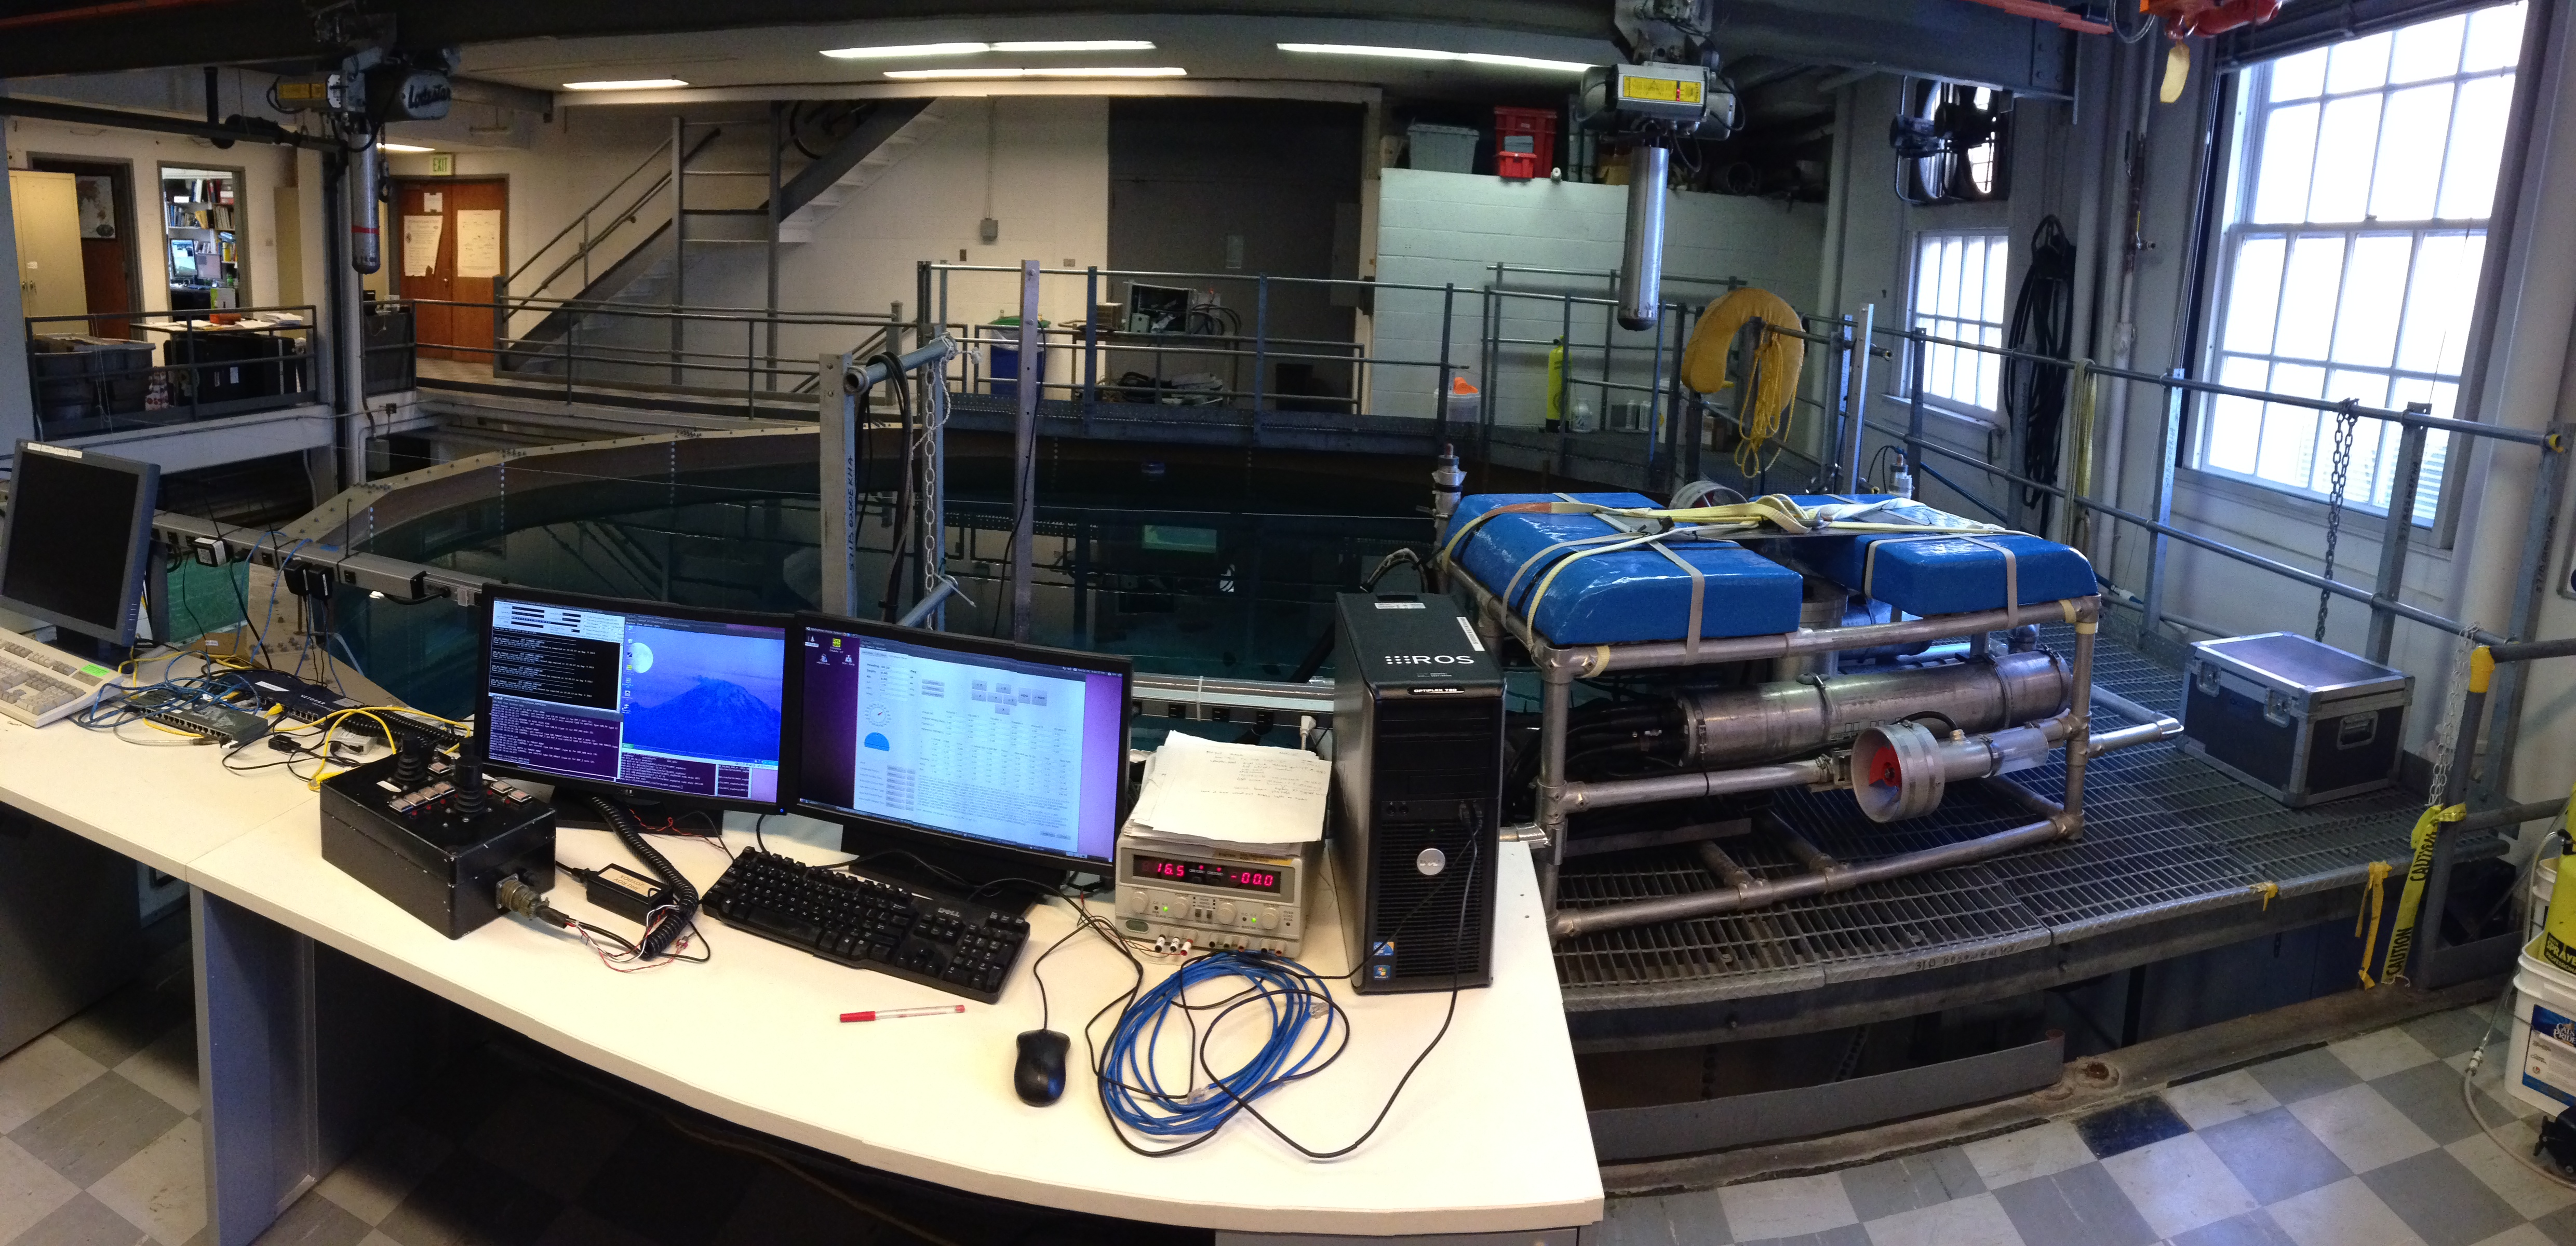
\includegraphics[trim=0mm 10cm 0mm 25cm,clip=true,width=\textwidth]{./appenJHUHTF/images/hydroFacility}
}
\\
\subfigure[\ac{JHUROV} starboard side view]  
{
    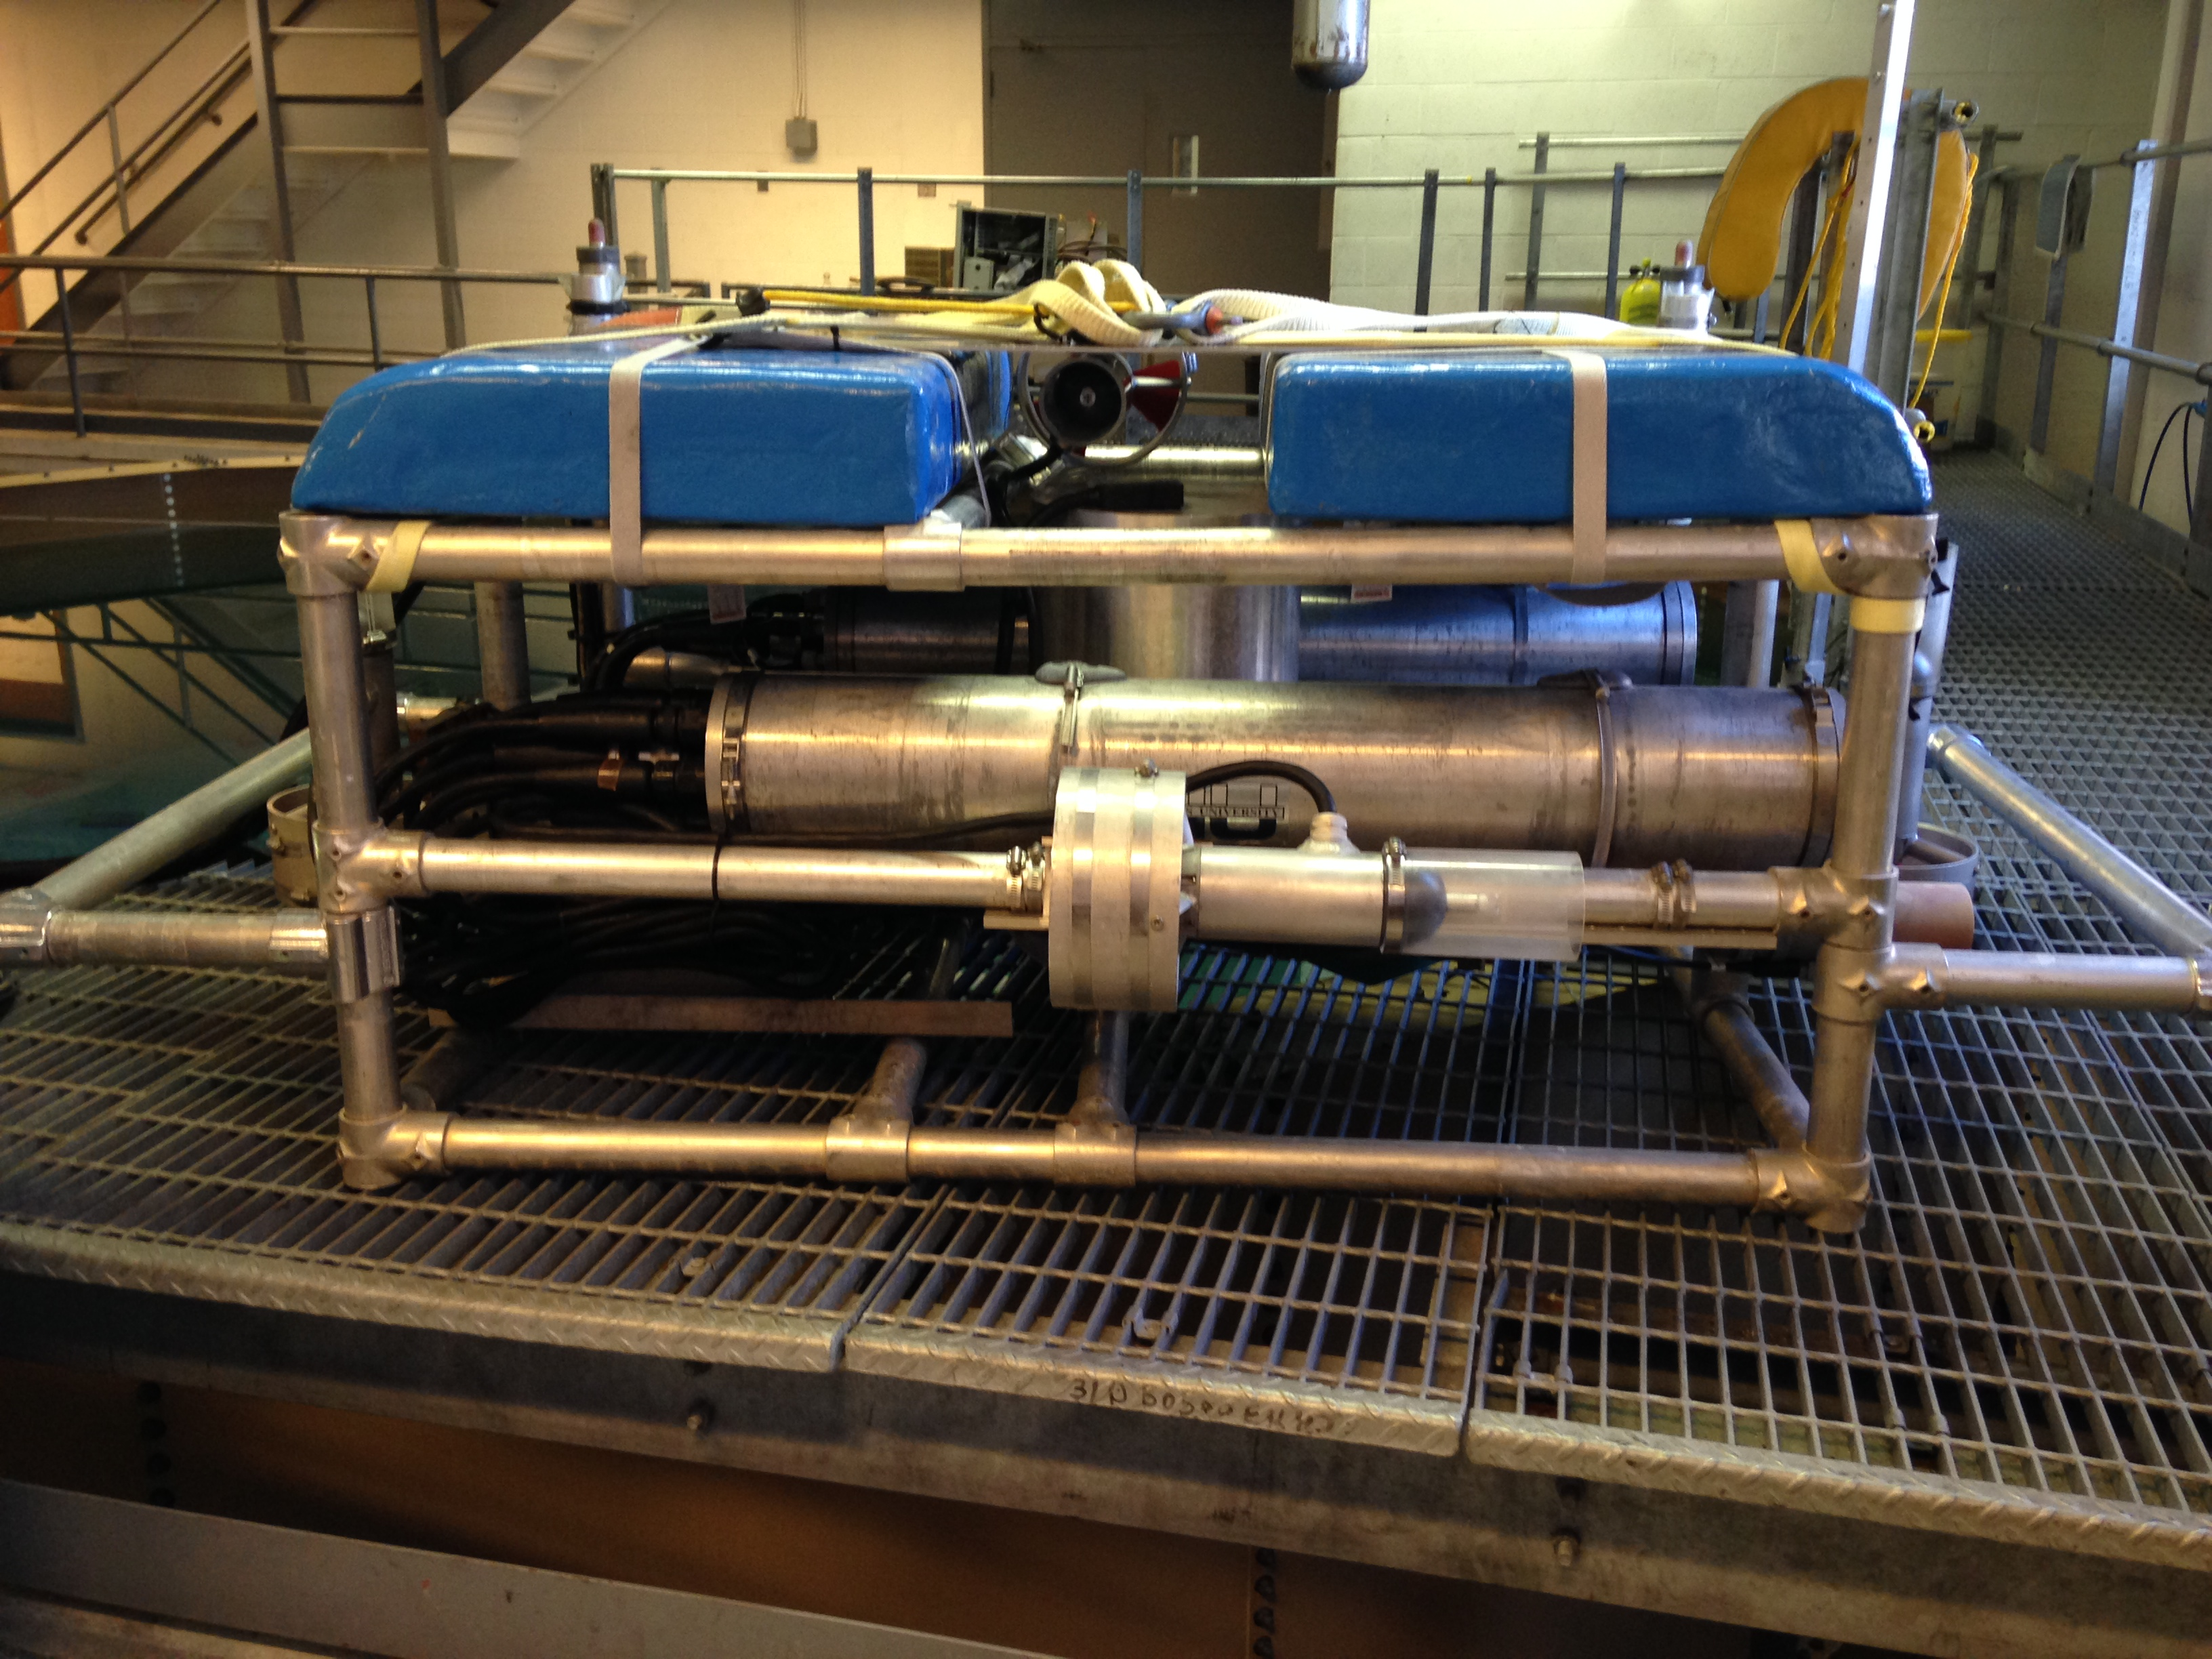
\includegraphics[trim=0mm 20cm 0mm 125mm,clip=true,width=.56\textwidth]{./appenJHUHTF/images/jhurovStarboard}
    %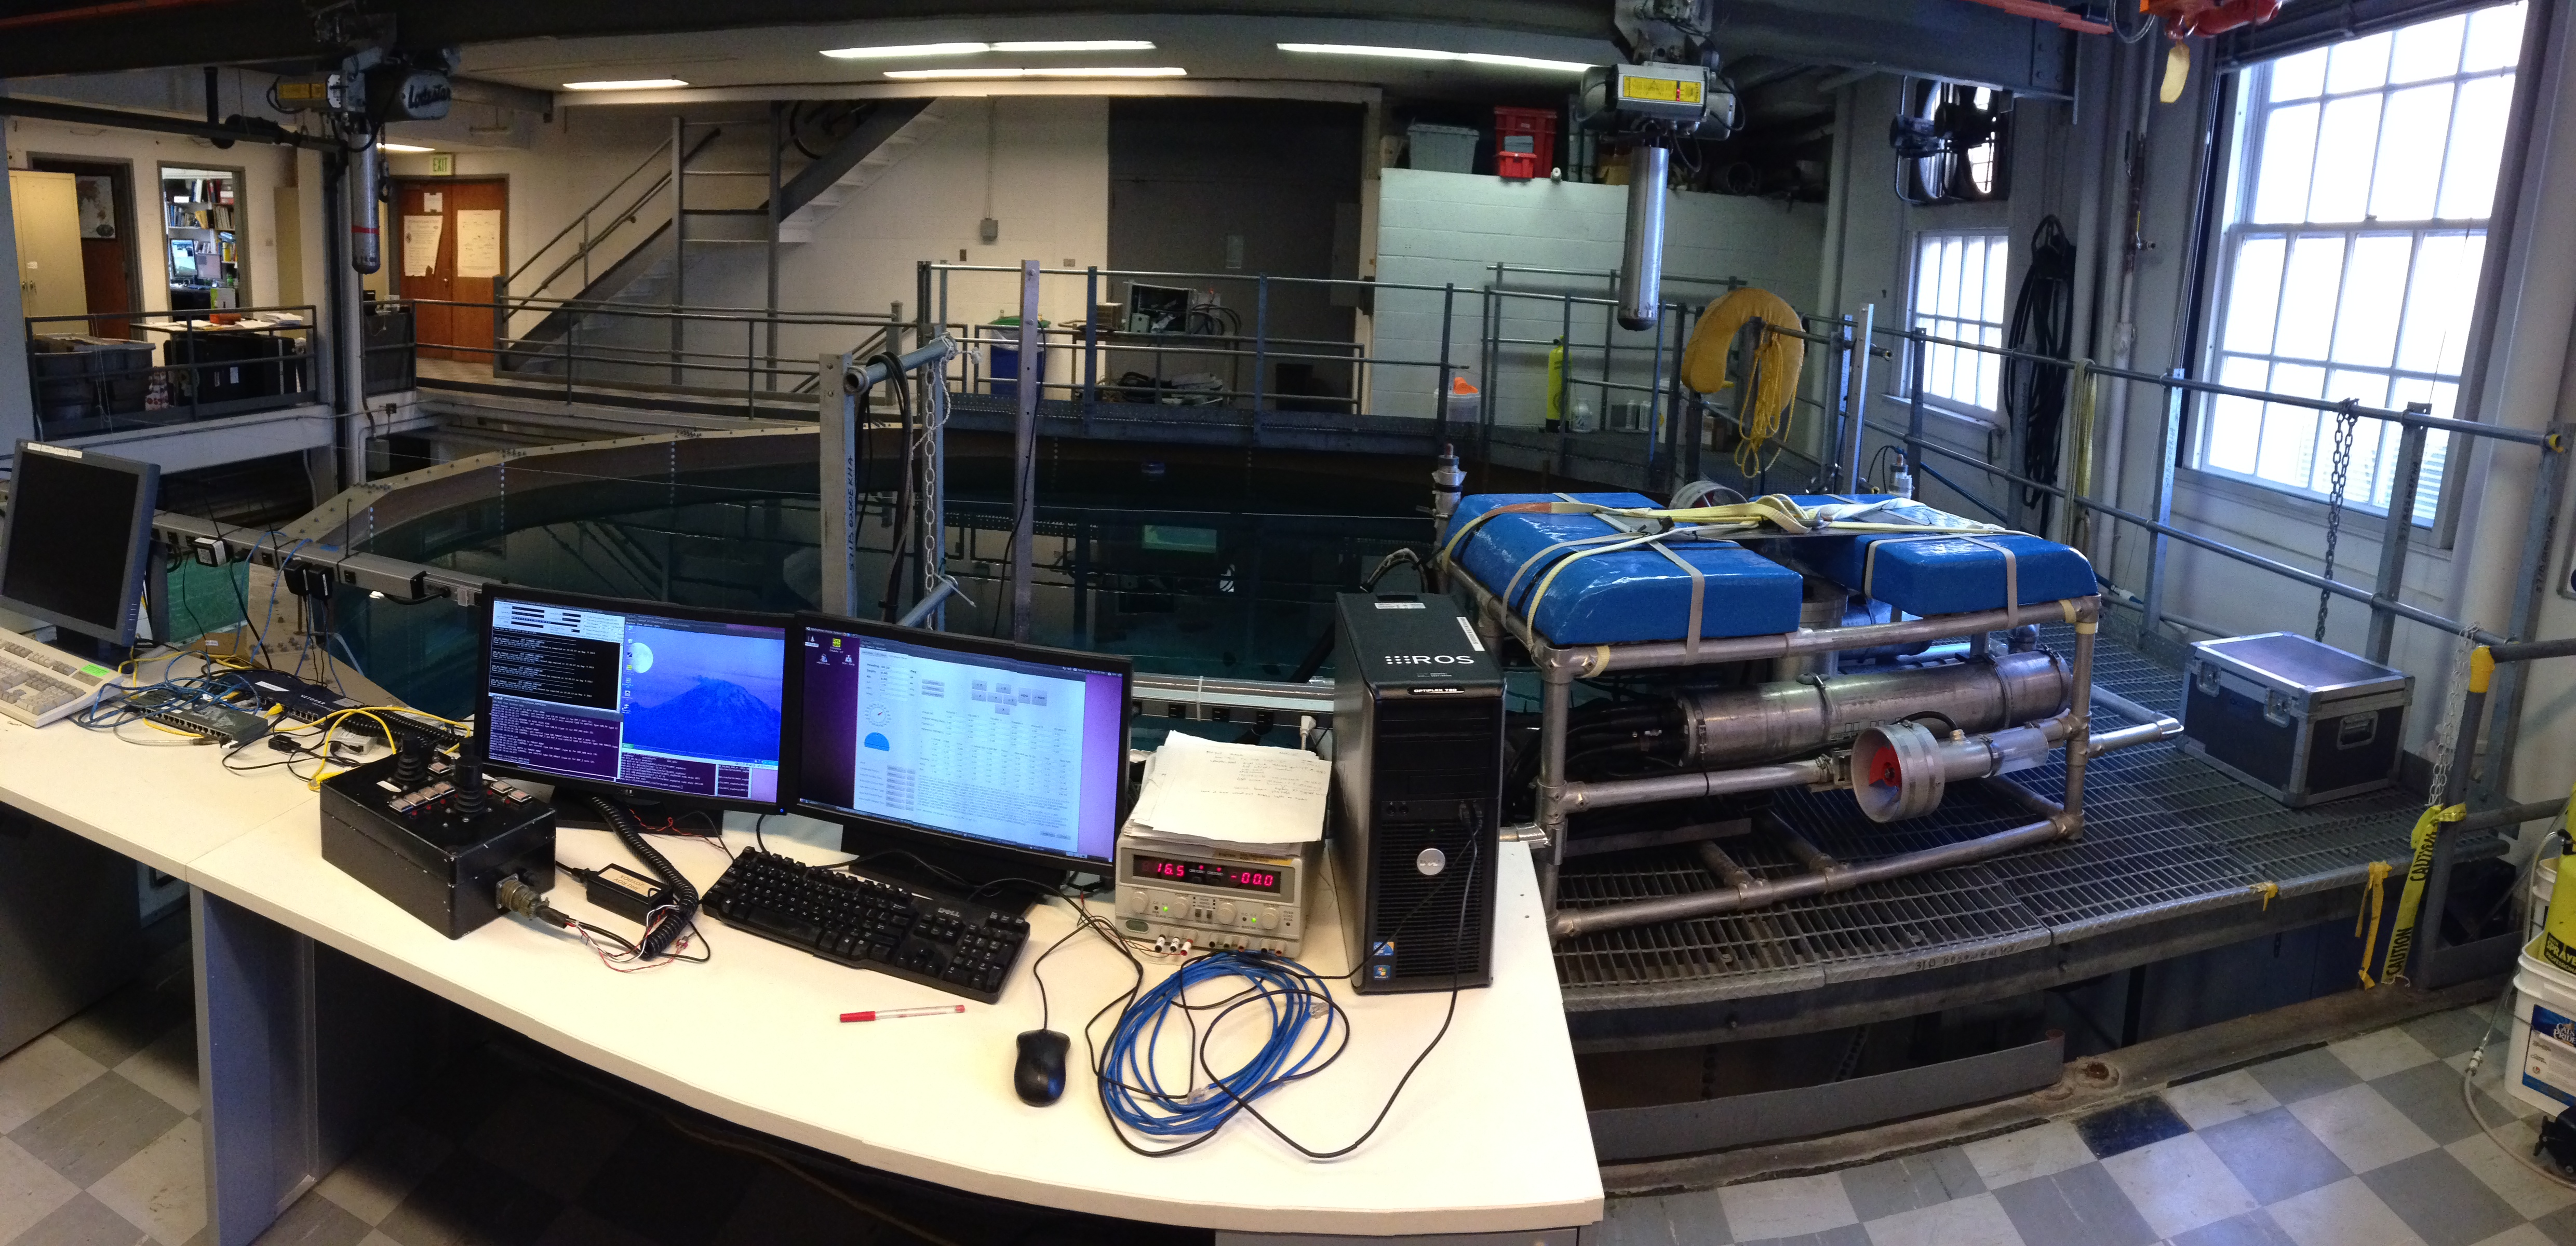
\includegraphics[width=170mm]{./appenJHUHTF/images/hydroFacility}
}
\subfigure[\ac{JHUROV} stern view] 
{
    %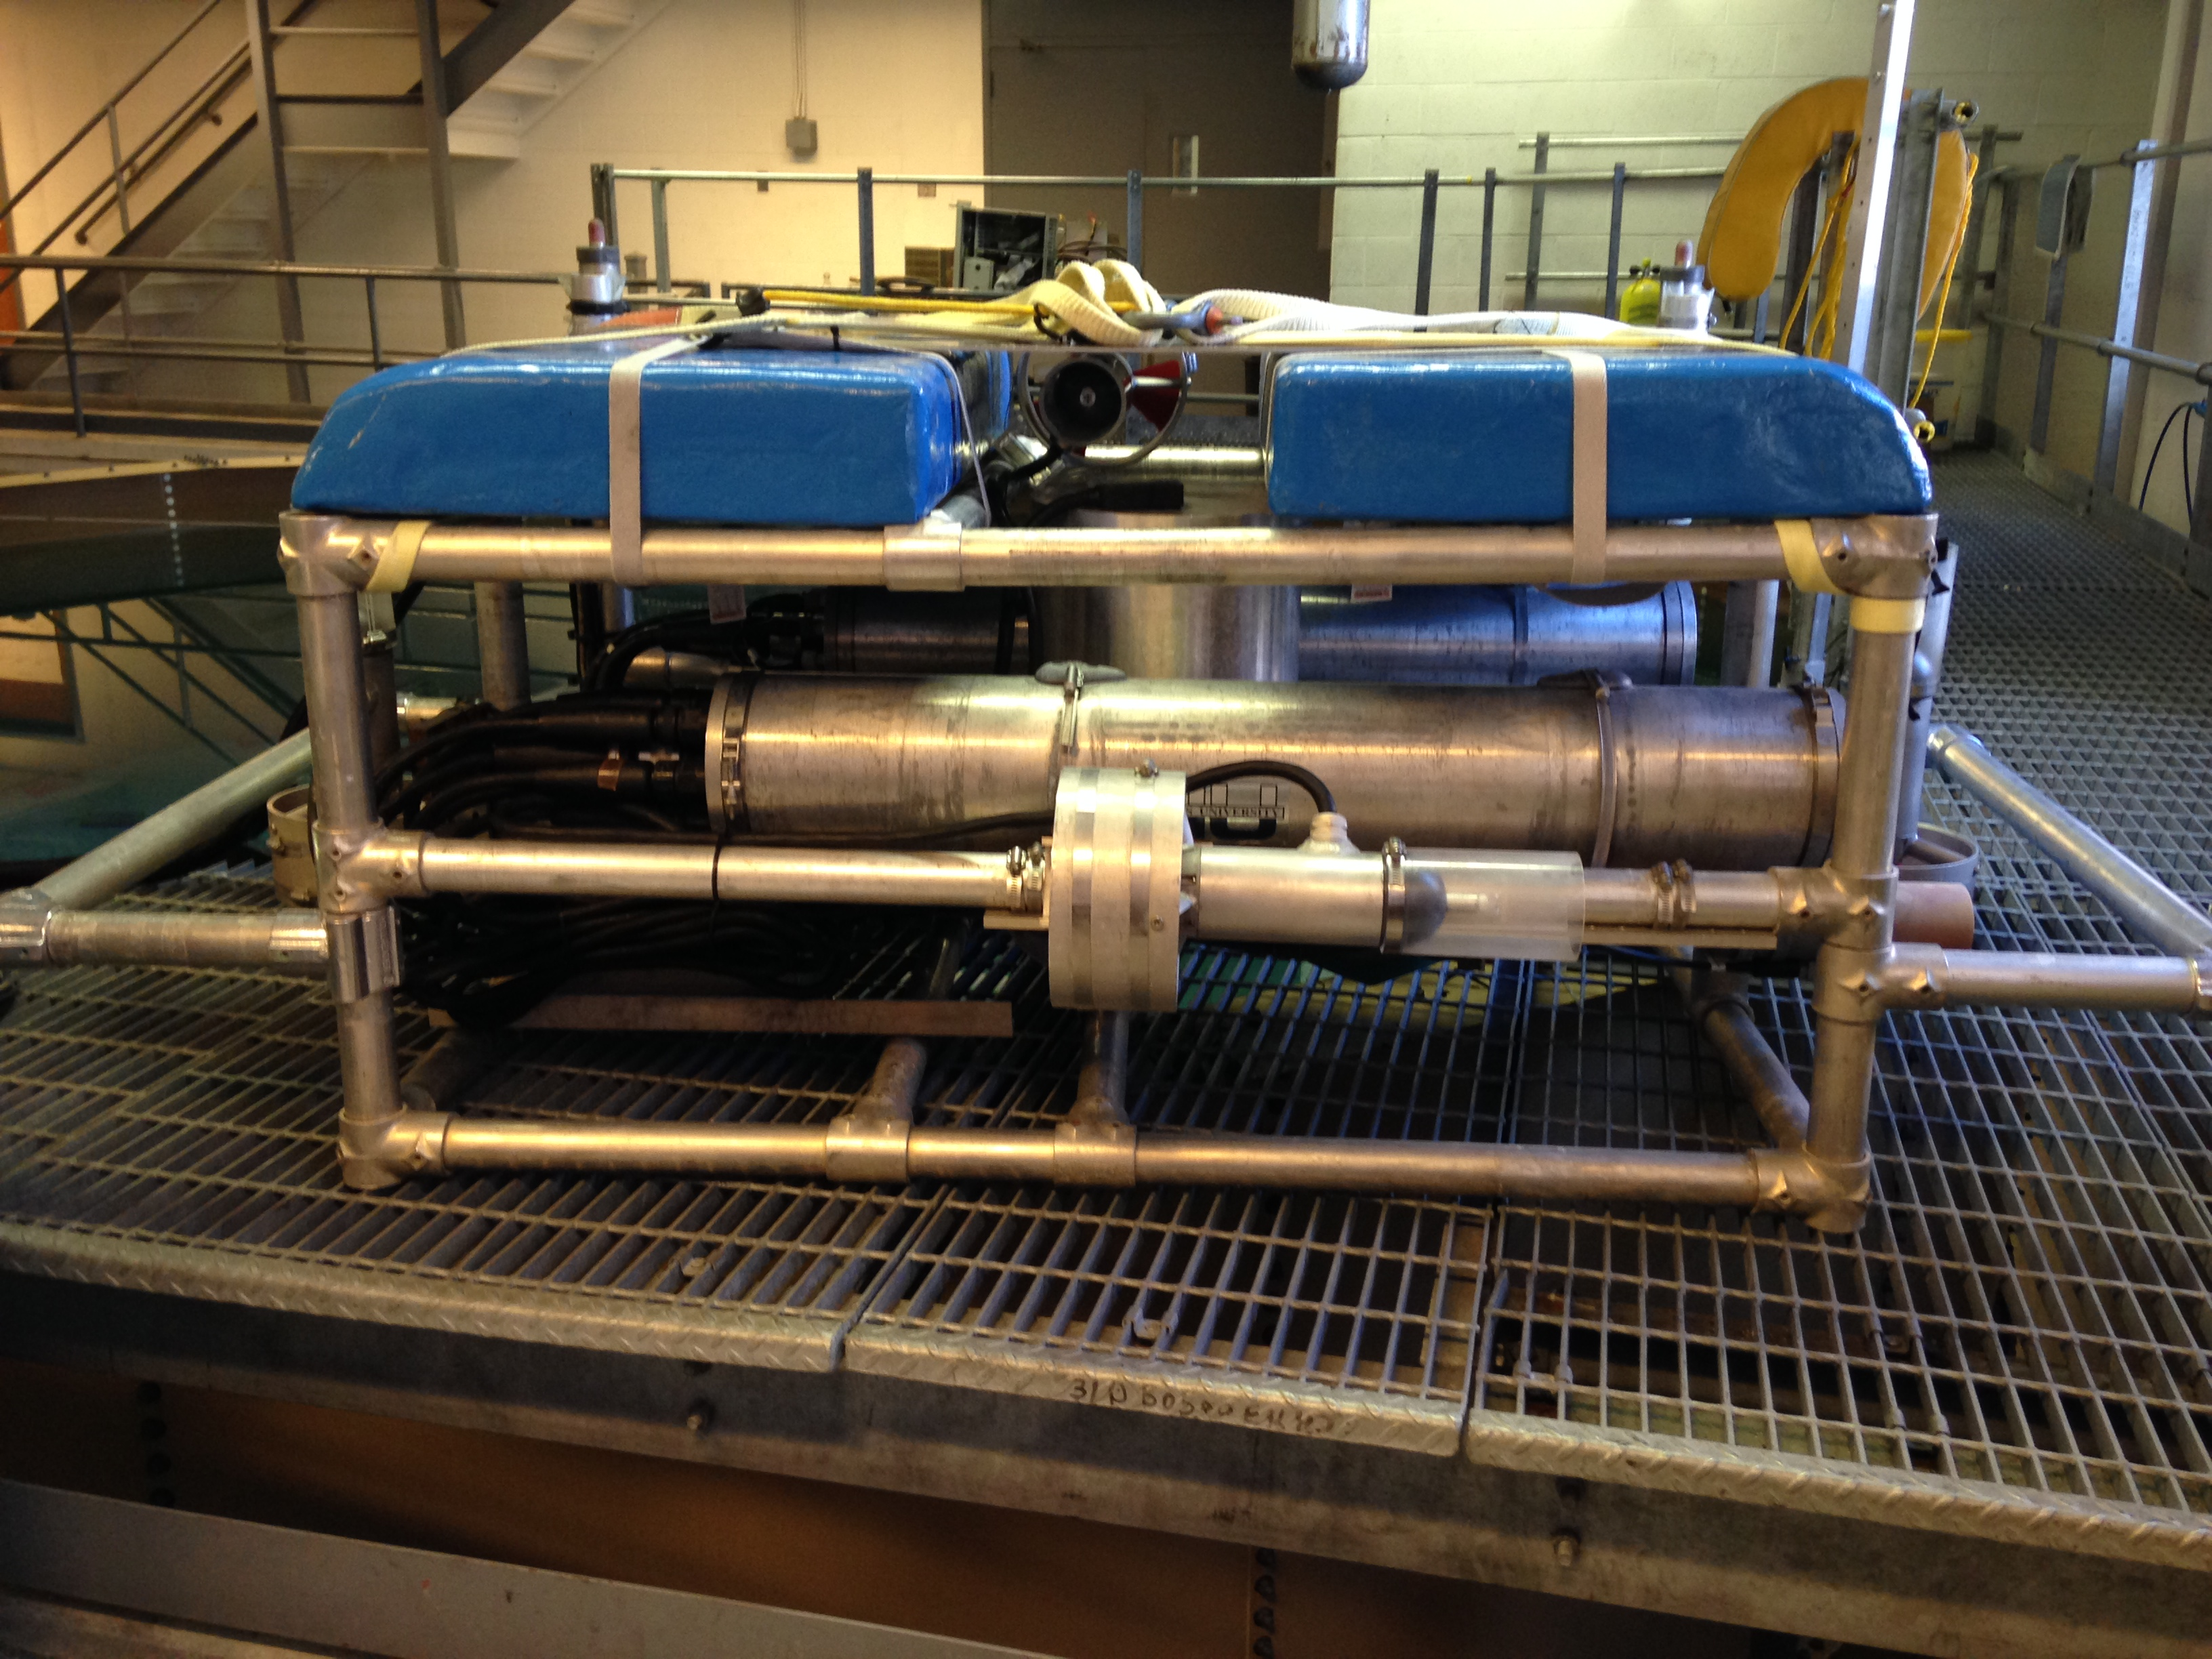
\includegraphics[trim=20cm 0mm 0mm 20cm,clip=true,width=80mm]{./appenJHUHTF/images/jhurovStarboard}
    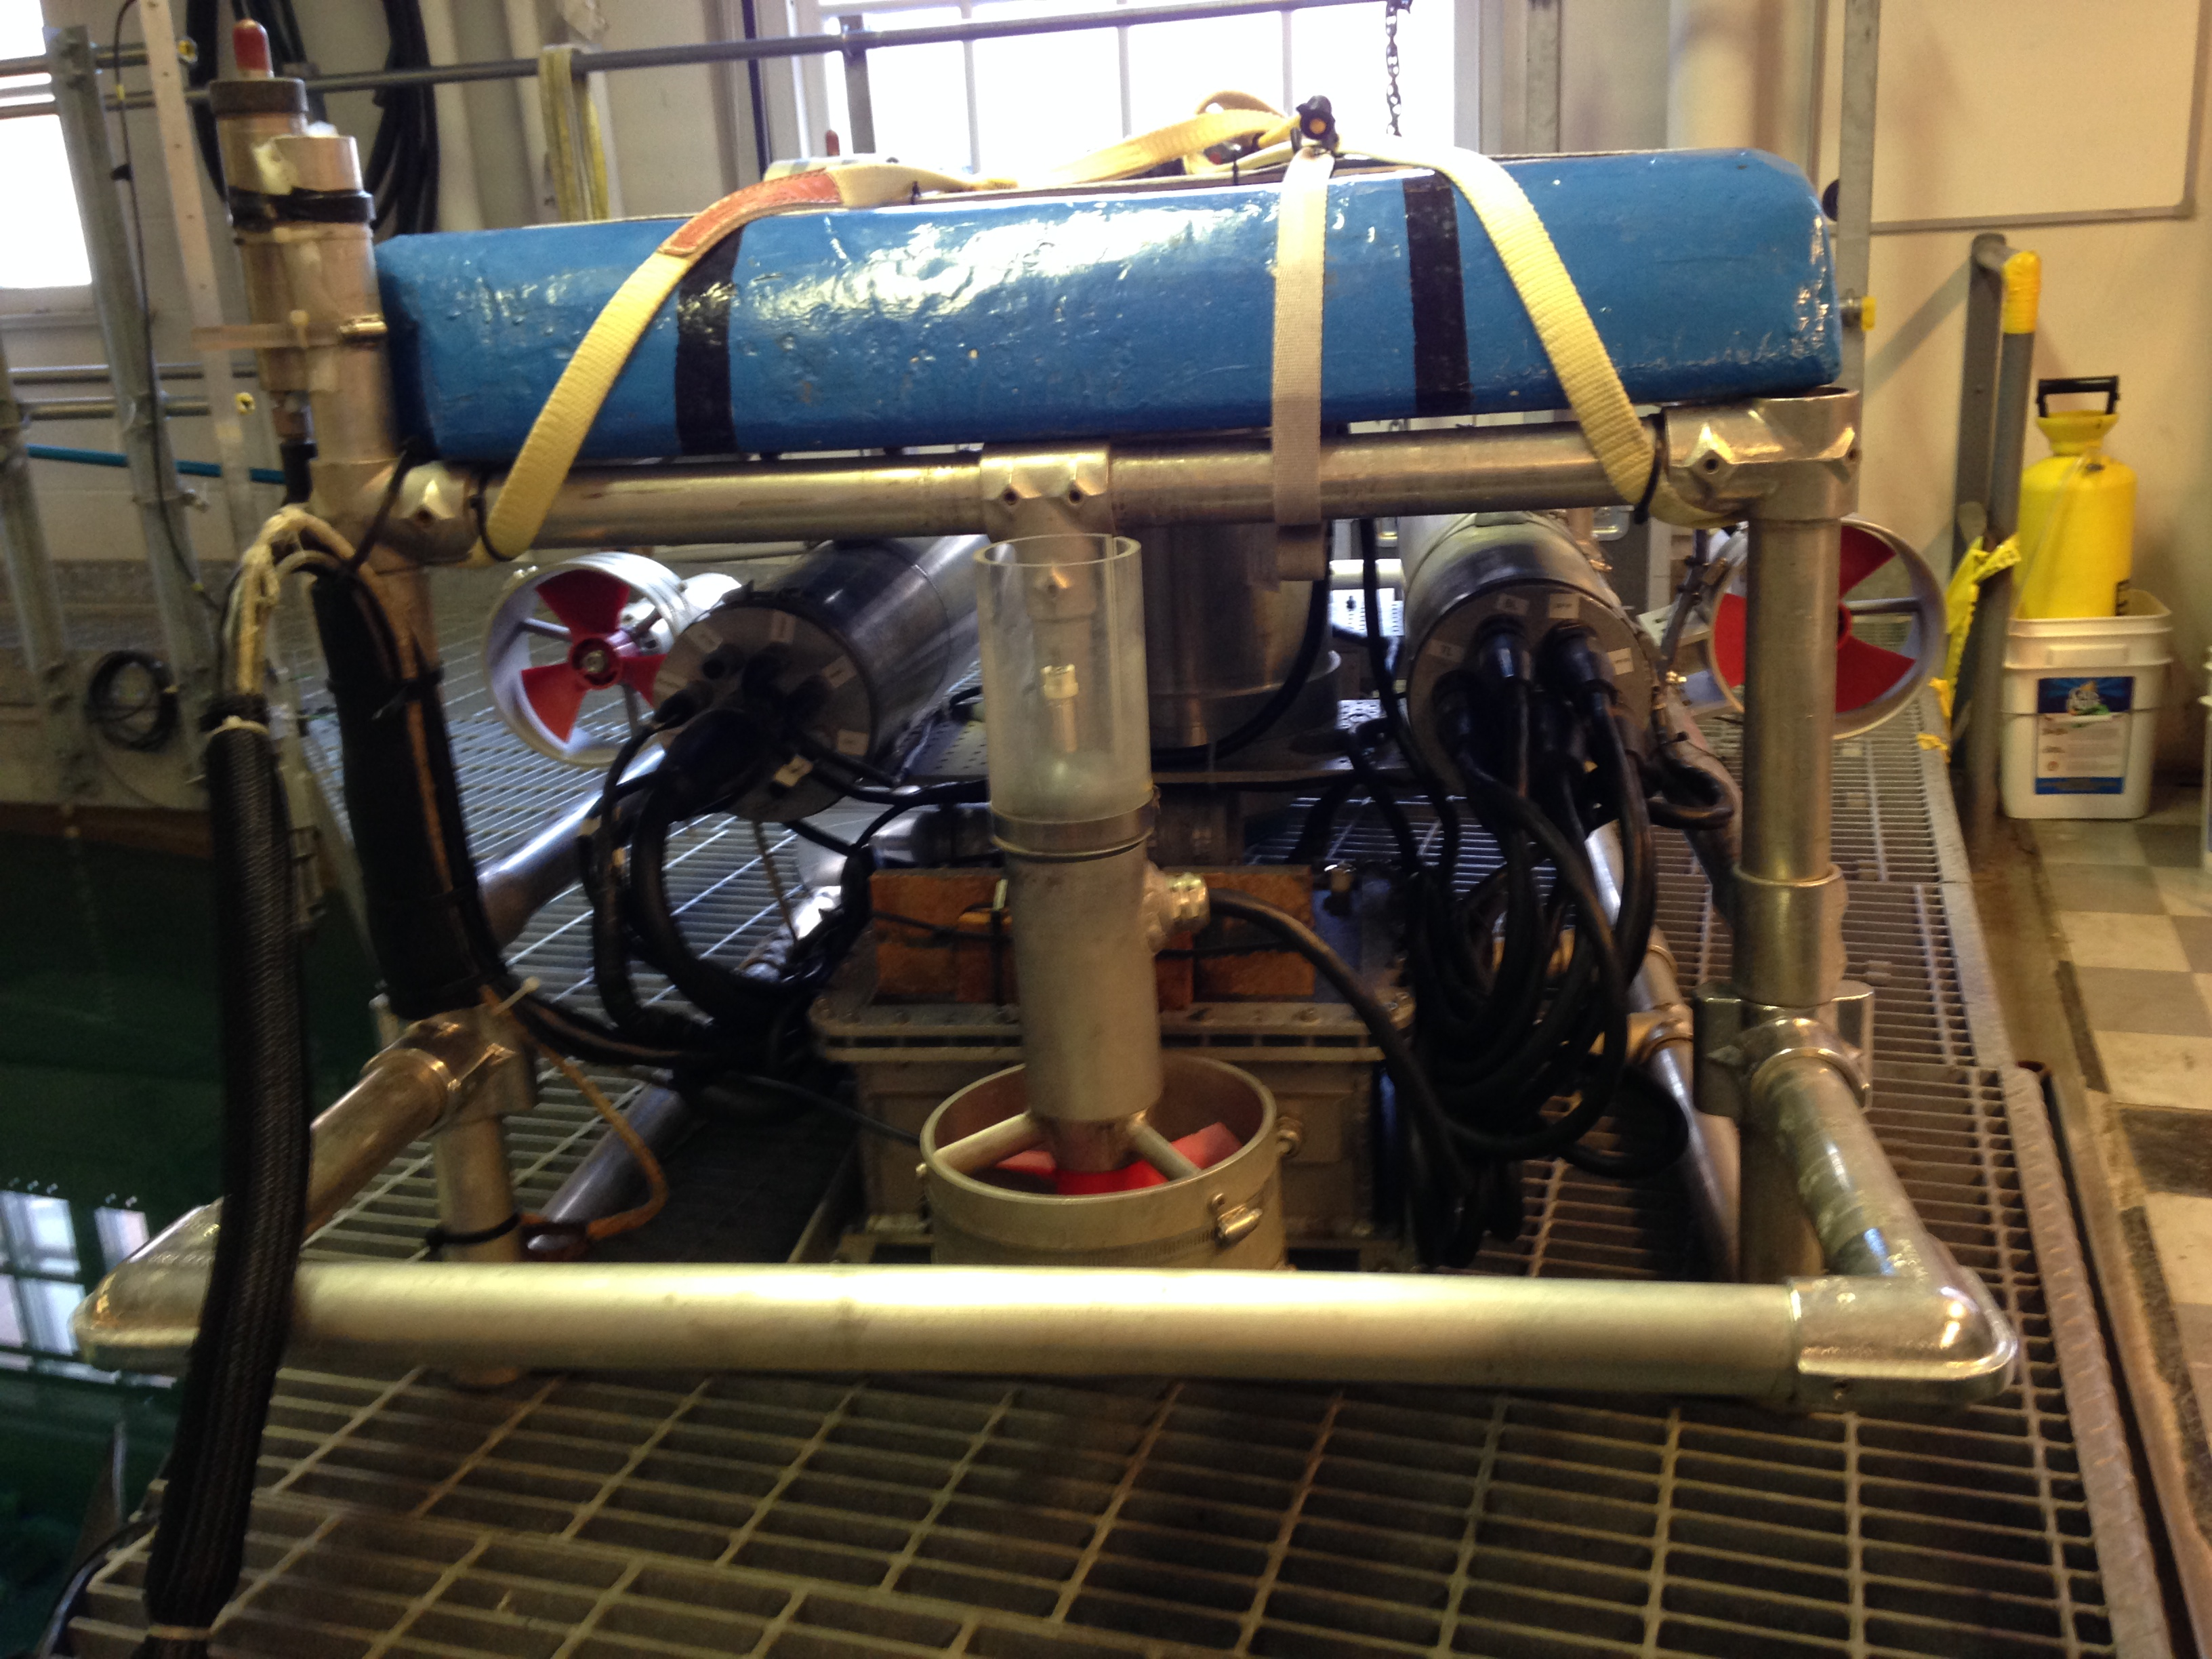
\includegraphics[trim=0mm 75mm 0mm 65mm,clip=true,width=.42\textwidth]{./appenJHUHTF/images/jhurovStern}
}
\caption{Johns Hopkins University Hydrodynamic Test Facility and \acf{JHUROV}.}
    \label{appenJHUHTF.fig.hydrolab}
\end{figure}
\end{center}


The Johns Hopkins Hydrodynamic Test Facility\cite{kinsey2003}
contains an indoor fresh water tank measuring \unit{7.75}{\m} in
diameter and \unit{4.25}{\m} deep, as shown in Figure
\ref{appenJHUHTF.fig.hydrolab}.  The facility is equipped with the
\ac{JHUROV}, a fully instrumented \ac{UV} designed for navigation and
control research.  The \ac{JHUROV} displaces \unit{150}{\kg} and is
actuated by six \unit{1.5}{\kWh} DC brushless electric direct drive
thrusters providing full control authority for 6-\ac{DOF}
maneuvers. Each thruster is controlled with a current-mode amplifier.
The \ac{JHUROV} control system generates the command current for each
thruster using data from {\it a-priori} {\it steady-state} thruster
calibration experiments; no feedback is used in generating the
commanded current.  The angular velocity of each thruster is
instrumented. This measured thruster angular velocity ($\omega_{th}$)
can be used to estimate the thruster force ($f_{th}$) using the
empirically validated steady state relation
$f_{th}=k_{th}\omega_{th}|\omega_{th}|$, where $k_{th}$ is an
empirically identified constant\cite{pona.book}.
%
The vehicle's control system is capable of actively controlling
6-\ac{DOF} vehicle motion.
%
During an experiment, each of the 6 \ac{JHUROV} \ac{DOF} were
independently actuated using either closed-loop control or open-loop
sinusoidal commanded torques. 
%
For the \acp{DOF} using closed-loop control,
a sinusoidal reference trajectory was specified to the \ac{JHUROV} control
system.



\begin{center}
\begin{figure}[htbp]
  \begin{center}
    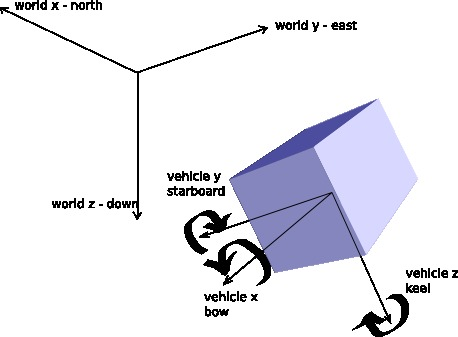
\includegraphics[width=90mm]{./appenJHUHTF/images/refFrames}
  \end{center}
  \caption{ The world-frame's orthonormal x, y, and z basis vectors
    point from the frame's origin towards in the directions north,
    east, and down respectively. The body-frame's orthonormal x, y, and
    z basis vectors point from the vehicles origin to the vehicle's
    bow side, starboard side and keel location respectively. Note the
    arrows showing positive rotation about each body axis.}
  \label{appenJHUHTF.fig.refFrames}
\end{figure}
\end{center}


The coordinate frames employed herein are depicted in Figure
\ref{appenJHUHTF.fig.refFrames}.
%
The world-frame's orthonormal x, y, and z basis vectors point from the
frame's origin towards the direction north, east, and down
respectively.
%
Employing standard navel architecture conventions, the body-frame's
orthonormal x, y, and z basis vectors point, respectively, from the
vehicle's origin to the vehicle's bow, starboard side and keel.
%
The Euler angles heading, pitch, and roll express the relationship
between the world-frame and body-frame as follows: rotating the world-frame
about its +z-axis through an angle heading, then rotating the resulting
frame about its +y-axis through an angle pitch, then rotating the
resulting-frame around its +x-axis through an angle roll provides the
body-frame.


\begin{table}[htbp]
\ssp
\caption{\ac{JHUROV} state measurement sources, resolutions, and accuracies}
\begin{center}
\begin{tabular}{cccc}
% & & RefTraj1& RefTraj2 \\
%\hline
%\multicolumn{2}{c}{Reference Trajectory}  &Trajectory Control      &  Parameter \\
%\multicolumn{2}{c}{Purpose}              & Evaluation &  Cross-Validation \\
 & &  & Measurement \\
State & Source  & Update Rate &Precision/Std Dev  \\
& & &(Standard Deviation)\\
\hline\hline
XY Translational  & DVLNAV    & \unit{10}{\Hz} & Resolution $>$0.5\% of\\
Position & & &Translational Distance Traveled \\
\hline
Z Translational   & Digiquartz & \unit{7}{\Hz} & Resolution \\
Position & & & $>$0.75\% as calculated \\
\hline
Heading                 & PHINS III & \unit{10}{\Hz}& 0.13$^\circ$ Std Dev \\  
\hline
Pitch, Roll             & PHINS III & \unit{10}{\Hz}& 0.01$^\circ$ Std Dev \\  
\hline
Translational  & \unit{1200}{\kHz}  & \unit{6}{\Hz} & $>$0.003 m/s Std Dev \\  
Velocity & \acs{DVL}& & \\
\hline
Angular Velocity        & PHINS III & \unit{10}{\Hz}& 0.01$^\circ$/s Std Dev \\  
\hline \hline\end{tabular}
\end{center}
\label{appen_JHUHTF.tb.sensors}
%\vspace*{-5mm}
\end{table}


The sensors used in all experimental evaluations are recorded in Table
\ref{appen_JHUHTF.tb.sensors}.  
%
The \ac{JHUROV} is instrumented by a PHINS III \ac{INS} (IXSEA SAS,
Marly-le-Roi, France), \unit{1200}{\kHz} bottom-lock Doppler sonar (RD
Instruments, San Diego, CA), and 8CDP010-1 Digiquartz Depth Sensor
(Paroscientific Inc., Redmond, WA).  
%
The PHINS III \ac{INS} includes a three-axis north-seeking fiber-optic
gyrocompass, and inertial grade accelerometers whose data is used to
estimate angular velocity, pitch, roll, and heading states at a rate
of \unit{10}{\Hz}.  
%
For our PHINS configuration, the measurement error standard deviations
are 0.01$^\circ$/s for angular velocity estimates, 0.13$^\circ$ for
heading estimates, and 0.01$^\circ$ for pitch and roll
estimates\cite{PhinsManual2008}. The Doppler sonar measures the three
dimensional linear velocity in the instrument's frame with a standard
deviation of less than 0.003 m/s, an update rate of \unit{6}{\Hz}, and
zero bias\cite{NWHdataSheet}.
%
The Digiquartz has a maximum depth of 10 m and, as currently
configured, has an update rate of \unit{7}{\Hz}, and provides pressure
measurements at a resolution of 2 parts-per-million.
%
Translational position estimates are provided by the DVLNAV control
software which integrates the the sensor signals reported above to
provide dead reckoning XY translational position estimates better than
0.5\% of distance traveled.
%








%\input{chUV_AID/expTestMeth}
%experimental.tex
\section{Experimental Evaluation: \\3-\acs{DOF}  \acs{UV} Rotational Dynamics \acs{AID}}
\label{chUV_AID.sec.UVSO3exp}

This Section reports a comparative experimental evaluation of \ac{AID}
and \ac{LS} for the estimation of plant parameters for the rotational
dynamics of a \ac{UV}.
%
We employed the Johns Hopkins University Hydrodynamic Test Facility to
evaluate each parameter identification method's capacity to identify
parameter sets which accurately model \ac{UV} dynamics.
%
The error between the predicted model performance and the
experimentally observed performance is reported as the \ac{MAE}
between the simulated plant roll, pitch, and velocities and the actual
experimental plant roll, pitch, and velocities.
%
Appendices \ref{appenJHUHTF.sec.hydrolab}
and \ref{appenJHUHTF.sec.paramEvalMethod} provide further details about
our experimental setup and parameter evaluation method.


At the beginning of each experiment, the vehicle was positioned in the
center of the tank with the vehicle's depth under closed loop control
at about a \unit{1}{\m} depth with the x and y \ac{DOF} unactuated.
%
During the experiment three sinusoidal torque commands (one in the
direction of each axis of the vehicle's coordinate frame) actuated the
angular position of the \ac{JHUROV}.
%
Table \ref{chUV_AID.tb.UVSE3expStat} shows the details of two exogenous
inputs, one for system identification and one for cross validation.
%
Hereafter we will refer to these experiments as the \ac{IDDAT} and the
\ac{CROSS} respectively.



\begin{table}[htbp]
\ssp
\caption{Exogenous Inputs for \ac{UV} Rotational Dynamics Parameter
  Identification Experiments}  
\begin{center}
\begin{tabular}{cccc}
\multicolumn{2}{c}{Experiment} & \ac{IDDAT} & \ac{CROSS} \\
\hline
\multicolumn{2}{c}{Experiment Purpose}  & Parameter      & Parameter  \\
               &                        & Identification & Cross-Validation \\
\hline
\multicolumn{2}{c}{Experiment Date}     & 2012-04-14    &   2012-04-09  \\ 
\hline
\multicolumn{2}{c}{Experiment Run Time} &  22.0 min     &   21.7 min    \\ 
\hline
Torque about &          Cos Freq          & 0.503 rad/sec & 0.583 rad/sec \\ 
X Vector     &          Cos Amp           &     40 N m    &     40 N m    \\ 
\hline
Torque about &          Cos Freq          & 0.663 rad/sec & 1.012 rad/sec \\ 
Y Vector     &          Cos Amp           &     55 N m    &     55 N m    \\ 
\hline
Torque about &          Cos Freq          & 1.043 rad/sec & 0.733 rad/sec \\ 
Z Vector     &          Cos Amp           &     70 N m    &     70 N m    \\ 
\hline \end{tabular}
\end{center}
\label{chUV_AID.tb.UVSO3expStat}
\end{table}



\begin{table*}[htbp]
\ssp
\caption{Numerical Values of the \ac{INITP} used to initialize \ac{UV} rotational dynamics \ac{AID}.}
\begin{center}
\begin{tabular}{c|c}
Parameter Symbol & \acf{INITP} \\ \hline
$\hat{I}(t_0)$ &
$ \left[\begin{array}{ccc} 100.0 & 0 & 0\\ 0 & 100.0 & 0\\ 0 & 0 & 100.0 \end{array}\right] $
\\
$\hat{C}_1(t_0)$ &
$ \left[\begin{array}{ccc} -100.0 & 0 & 0\\ 0 & -100.0 & 0\\ 0 & 0 & -100.0 \end{array}\right] $
\\
$\hat{C}_2(t_0)$ &
$ \left[\begin{array}{ccc} -100.0 & 0 & 0\\ 0 & -100.0 & 0\\ 0 & 0 & -100.0 \end{array}\right] $
\\
$\hat{C}_3(t_0)$ &
$ \left[\begin{array}{ccc} -100.0 & 0 & 0\\ 0 & -100.0 & 0\\ 0 & 0 & -100.0 \end{array}\right] $
\\
$\hat{b}(t_0)$ &
$ \left[\begin{array}{c} 0\\ 0\\ 100.0 \end{array}\right] $
\\
\end{tabular}
\end{center}
\label{chUV_AID.tb.UVSO3_INIT_params}
\end{table*}



\ac{AID} was implemented as a discrete time approximation of the
continuous time algorithm.  
%
%Once every 100ms the most recent state measurements, commanded torque,
%parameter estimates, and angular velocity estimate were used to
%calculate the angular velocity and parameter estimate derivatives
%(\ref{chUV_AID.eq.UV_SO3_Estimator})-(\ref{chUV_AID.eq.UV_SO3_BuoyId}).
%
Euler integration of (\ref{chUV_AID.eq.UV_SO3_Estimator})---(\ref{chUV_AID.eq.UV_SO3_BuoyId})
for 100ms time steps
provided the time series of parameter and angular velocity
estimates.
%
100ms is one to two orders-of-magnitude smaller than the state signal
variation rates of 1 second or greater observed during quasi-periodic
\ac{JHUROV} operations.
%
The experiments were designed to generate thruster commands varying
slowly enough to admit the use of steady state thruster models.
%
In practice, first-order Euler integration provided performance
similar to the 4th-order integration implemented in simulation.



The \ac{AID} algorithm was initialized with the measured angular position,
measured angular velocity, and \acf{INITP} in Table
\ref{chUV_AID.tb.UVSO3_INIT_params}.
%
Note that the \ac{INITP} was chosen such that each scalar
parameter was within an order-of-magnitude of the value to be identified.
%
The choice of optimal adaptation gains is a long-standing open problem
in adaptive systems theory\cite{Nguyen-2009,ksn&anu.book}.
%
From simulations of this \ac{AID} algorithm which sparsely covered a 
roughly logarithmic scaling for a range of possible gains, we
empirically chose angular velocity, inertia tensor, quadratic drag,
and buoyancy torque adaption gains of $a=10$, $\gamma_1=5000$,
$\gamma_2=10000$, and $\gamma_3=1000$ respectively.
%
Many of the gain combinations considered provided parameter
convergence rates comparable to the gains used herein.
%
Our simulation studies suggest similar results would be obtained for
initial condition and gain choices within an order-of-magnitude of the
choices made.





\subsection{Experimental Results}%\label{ref.expResults}


The state measurements from the \ac{IDDAT} dataset were used to
identify the plant parameters of the plant model
(\ref{chModels.eq.UVSO3plant}) with both the adaptive identification
and least squares methods.
%
Table \ref{chUV_SO3.tb.UVSO3_ID_params} reports two identified
parameter sets: the \acf{AIDP} estimated with \ac{AID} (as per Section
\ref{chUV_AID.sec.UV_SO3_AID}) and the \acf{LSP} estimated with
\ac{LS} (as per Section \ref{chUV_AID.sec.leastSquares}). 
%TM_CHECK could cut out the 'as per' parenthetal statements above 
%

The parameter sets \ac{AIDP},  \ac{LSP}, and \ac{INITP} were used as
parameter sets for three \ac{UV} rotational dynamics models; the
\acf{AIDPM}, the \acf{LSPM}, and the \acf{INITPM}.
%
Using the torque input commands from the \ac{IDDAT} and \ac{CROSS}
datasets, we compare simulated \ac{JHUROV} performance from numerical
simulations of \ac{AIDPM}, \ac{LSPM}, and \ac{INITPM} to the measured
\ac{JHUROV} states for each experiment respectively.

Using the torque inputs from the \ac{CROSS} dataset, Figures
\ref{chUV_AID.fig.SO3_INIT_pos} --- \ref{chUV_AID.fig.SO3_AID_vel}
compare the state measurements from simulations of \ac{AIDPM},
\ac{LSPM}, and \ac{INITPM} to the measured \ac{JHUROV} states from
the \ac{CROSS} dataset.
%
%The \ac{JHUROV} simulation in Figures \ref{chUV_AID.fig.SO3_INIT_pos}
%and \ref{chUV_AID.fig.SO3_INIT_vel} use the \ac{INITP} to model
%vehicle dynamics.  
%
%In a similar fashion, Figures \ref{chUV_AID.fig.SO3_AID_pos} and
%\ref{chUV_AID.fig.SO3_INIT_vel} plot data from two \ac{JHUROV}
%simulations, using either the \ac{AIDP} or \ac{LSP} to model vehicle
%dynamics.
%
Each of these four Figures display three minute subsets of the 20 minutes of
state data generated by driving simulations of \ac{AIDPM},
\ac{LSPM}, and \ac{INITPM} using the torque data from the \ac{CROSS}
dataset.
%
Similar simulations of \ac{AIDPM}, \ac{LSPM}, and \ac{INITPM} were
created using the torque commands from the \ac{IDDAT} dataset.
%
Table \ref{chUV_AID.tb.SO3_MAE} summarizes the \ac{MAE} between
measured and simulated vehicle state for each experimental dataset,
%(\ac{IDDAT} or \ac{CROSS)), 
\ac{UV} vehicle model, 
%(\acf{AIDPM}, \acf{LSPM}, and \ac{INITPM}), 
and open-loop-stable \ac{DOF}.
%(roll, pitch and agular velocities).


\begin{table}[htbp]
\ssp
\caption{\acfp{MAE} between measured and simulated vehicle states for all pairs of 
  \ac{UV} rotational dynamics experiments and \ac{UV} rotational dynamics models.}
\begin{center}
\begin{tabular}{c|cccccc}
\ac{UV} & & \multicolumn{2}{c}{Angular Pose} & \multicolumn{3}{c}{Angular Velocity} \\ 
 Model & Experiment & Roll & Pitch & x \ac{DOF} & y \ac{DOF} & z \ac{DOF} \\ \hline
\ac{AIDPM}  & \ac{CROSS} & 4.11$^\circ$ & 2.88$^\circ$ & 6.16$^\circ$/s & 2.83$^\circ$/s & 3.44$^\circ$/s \\
\ac{LSPM}   & \ac{CROSS} & 2.50$^\circ$ & 2.65$^\circ$ & 3.36$^\circ$/s & 3.69$^\circ$/s & 5.46$^\circ$/s \\
\ac{INITPM} & \ac{CROSS} & 13.3$^\circ$ & 14.6$^\circ$ & 8.86$^\circ$/s & 12.9$^\circ$/s & 7.00$^\circ$/s \\
\ac{AIDPM}  & \ac{IDDAT} & 3.44$^\circ$ & 2.06$^\circ$ & 4.80$^\circ$/s & 1.99$^\circ$/s & 4.03$^\circ$/s \\
\ac{LSPM}   & \ac{IDDAT} & 2.08$^\circ$ & 1.76$^\circ$ & 2.45$^\circ$/s & 2.19$^\circ$/s & 5.05$^\circ$/s \\
\ac{INITPM} & \ac{IDDAT} & 14.8$^\circ$ & 17.1$^\circ$ & 8.83$^\circ$/s & 10.7$^\circ$/s & 6.32$^\circ$/s \\
\end{tabular}
\end{center}
\label{chUV_AID.tb.SO3_MAE}
\end{table}

\begin{table*}[htbp]
\ssp
\caption{The \ac{UV} rotational dynamics parameter sets identified
  using the \ac{IDDAT} dataset.}
\begin{center}
\begin{tabular}{c|cc}
Parameter Symbol & \ac{AIDP} & \ac{LSP} \\ \hline
$\hat{I}(t_f)$ &
$ \left[\begin{array}{ccc} 136.0 & -12.7 & 2.89\\ -12.7 & 175.0 & -1.06\\ 2.89 & -1.06 & 160.0 \end{array}\right] $
&
$ \left[\begin{array}{ccc} 31.9 & -5.04 & 1.53\\ -5.04 & 55.9 & -6.19\\ 1.53 & -6.19 & 96.3 \end{array}\right] $
\\
$\hat{C}_1(t_f)$ &
$ \left[\begin{array}{ccc} -215.0 & 19.1 & 21.3\\ -23.0 & -243.0 & -10.1\\ 7.16 & -80.9 & -129.0 \end{array}\right] $
&
$ \left[\begin{array}{ccc} -297.0 & 4.14 & 1.32\\ 7.6 & -414.0 & -28.1\\ 150.0 & -165.0 & 52.3 \end{array}\right] $
\\
$\hat{C}_2(t_f)$ &
$ \left[\begin{array}{ccc} -137.0 & 39.8 & 46.5\\ -14.0 & -367.0 & -39.2\\ 15.0 & -117.0 & -186.0 \end{array}\right] $
&
$ \left[\begin{array}{ccc} -358.0 & 13.7 & 13.0\\ 91.8 & -266.0 & -20.5\\ 107.0 & -181.0 & -80.2 \end{array}\right] $
\\
$\hat{C}_3(t_f)$ &
$ \left[\begin{array}{ccc} -80.6 & 38.4 & -17.3\\ -2.0 & -287.0 & 19.6\\ 37.0 & -52.1 & -214.0 \end{array}\right] $
&
$ \left[\begin{array}{ccc} 3.4 & 18.9 & -9.58\\ -9.27 & -262.0 & 18.2\\ -70.0 & 34.8 & -252.0 \end{array}\right] $
\\
$\hat{b}(t_f)$ &
$ \left[\begin{array}{c} 1.57\\ -1.5\\ 277.0 \end{array}\right] $
&
$ \left[\begin{array}{c} 1.38\\ 1.11\\ 235.0 \end{array}\right] $
\\
\end{tabular}
\end{center}
\label{chUV_SO3.tb.UVSO3_ID_params}
\end{table*}


\begin{center}
\begin{figure}[htbp]
  \begin{center}
    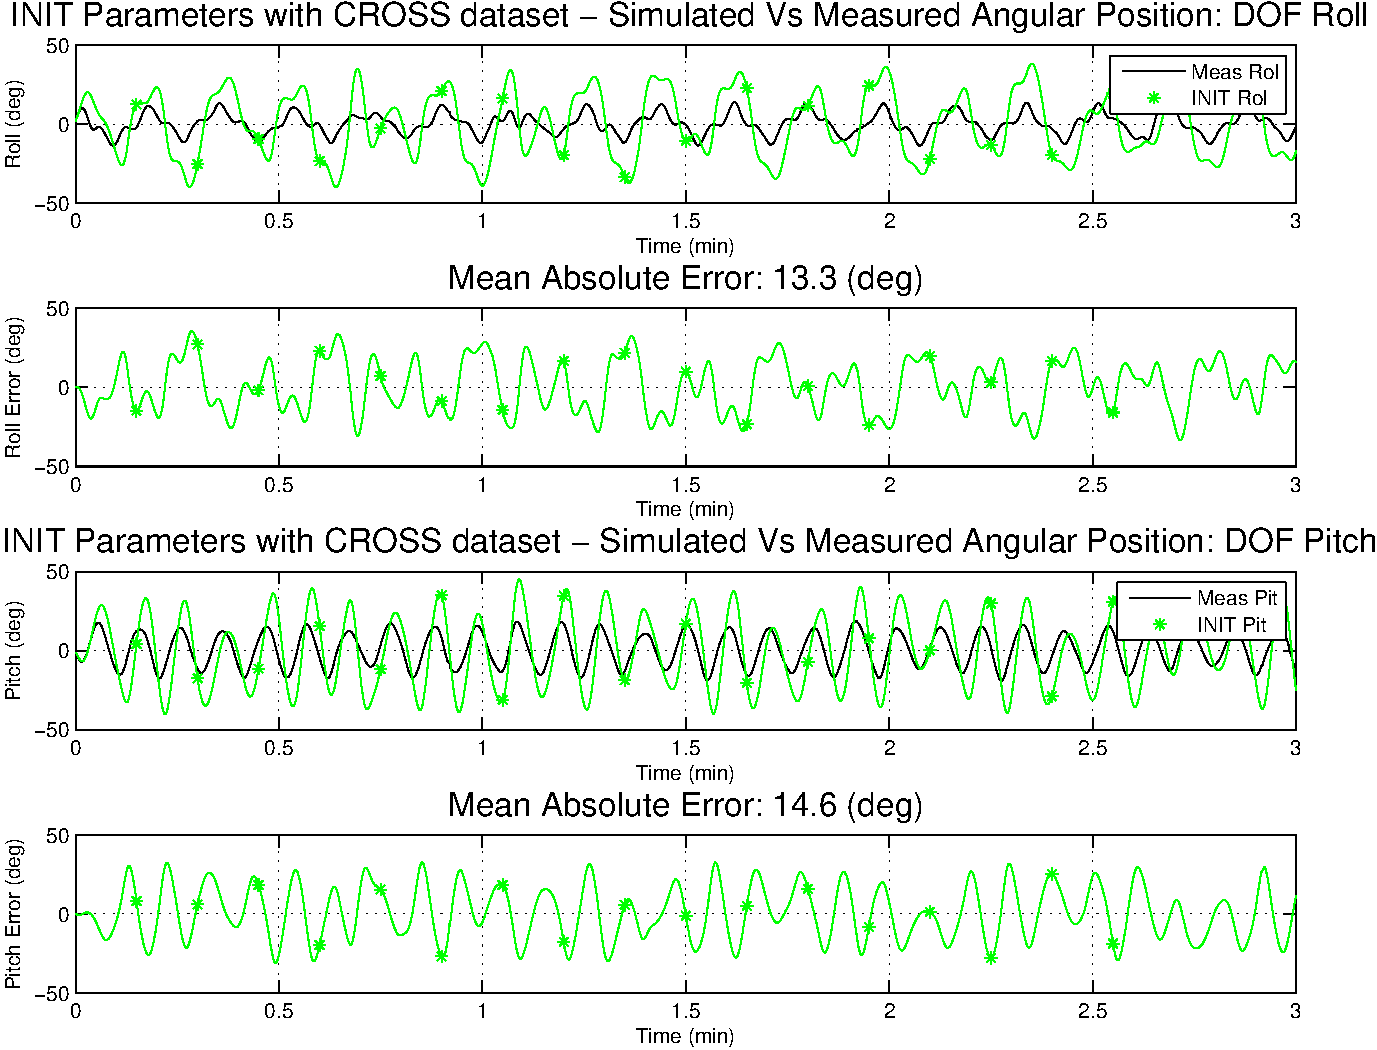
\includegraphics[width=6in]{./chUV_AID/images/crossINIT_pos}
  \end{center}
  \caption{ Representative data of experimental and simulated
    \ac{JHUROV} angular position for the \ac{CROSS} dataset. In the
    roll and pitch plots, the measured states are plotted together
    with the states from simulating \ac{INITPM}.  For each \ac{DOF},
    the difference between the measured position and simulated
    position is shown. 
%The \ac{INITP} was chosen to arbitrary
%    initialize the \ac{AID} algorithm, thus the large errors between
%    the simulated and measured angular positions of the \ac{JHUROV}
%    demonstrate there exists parameter sets which poorly characterize
%    the \acp{UV} performance.
}
  \label{chUV_AID.fig.SO3_INIT_pos}
\end{figure}
\end{center}

\begin{center}
\begin{figure}[htbp]
  \begin{center}
    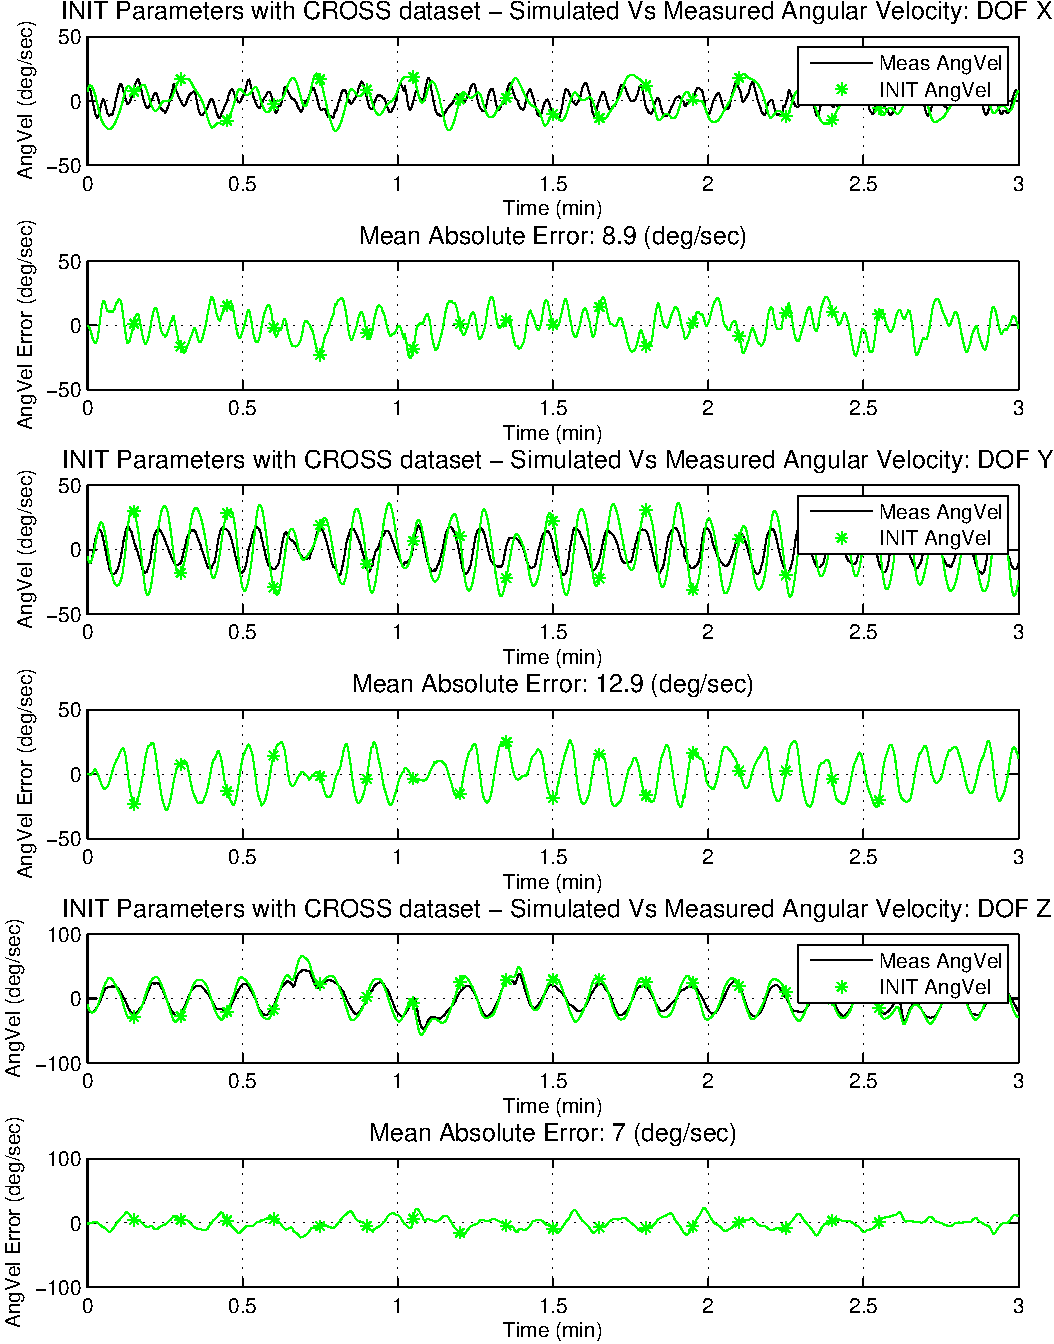
\includegraphics[width=5.5in]{./chUV_AID/images/crossINIT_vel}
  \end{center}
  \caption{ Representative data of experimental and simulated
    \ac{JHUROV} angular velocity for the \ac{CROSS} dataset. In the
    individual angular velocity plots, each measured velocity is
    plotted together with the states from simulating \ac{INITPM}.  For
    each \ac{DOF} error plots are also included. 
    %See the caption of
%    Figure \ref{chUV_AID.fig.SO3_INIT_pos} for further information.
}
  \label{chUV_AID.fig.SO3_INIT_vel}
\end{figure}
\end{center}

\begin{center}
\begin{figure}[htbp]
  \begin{center}
    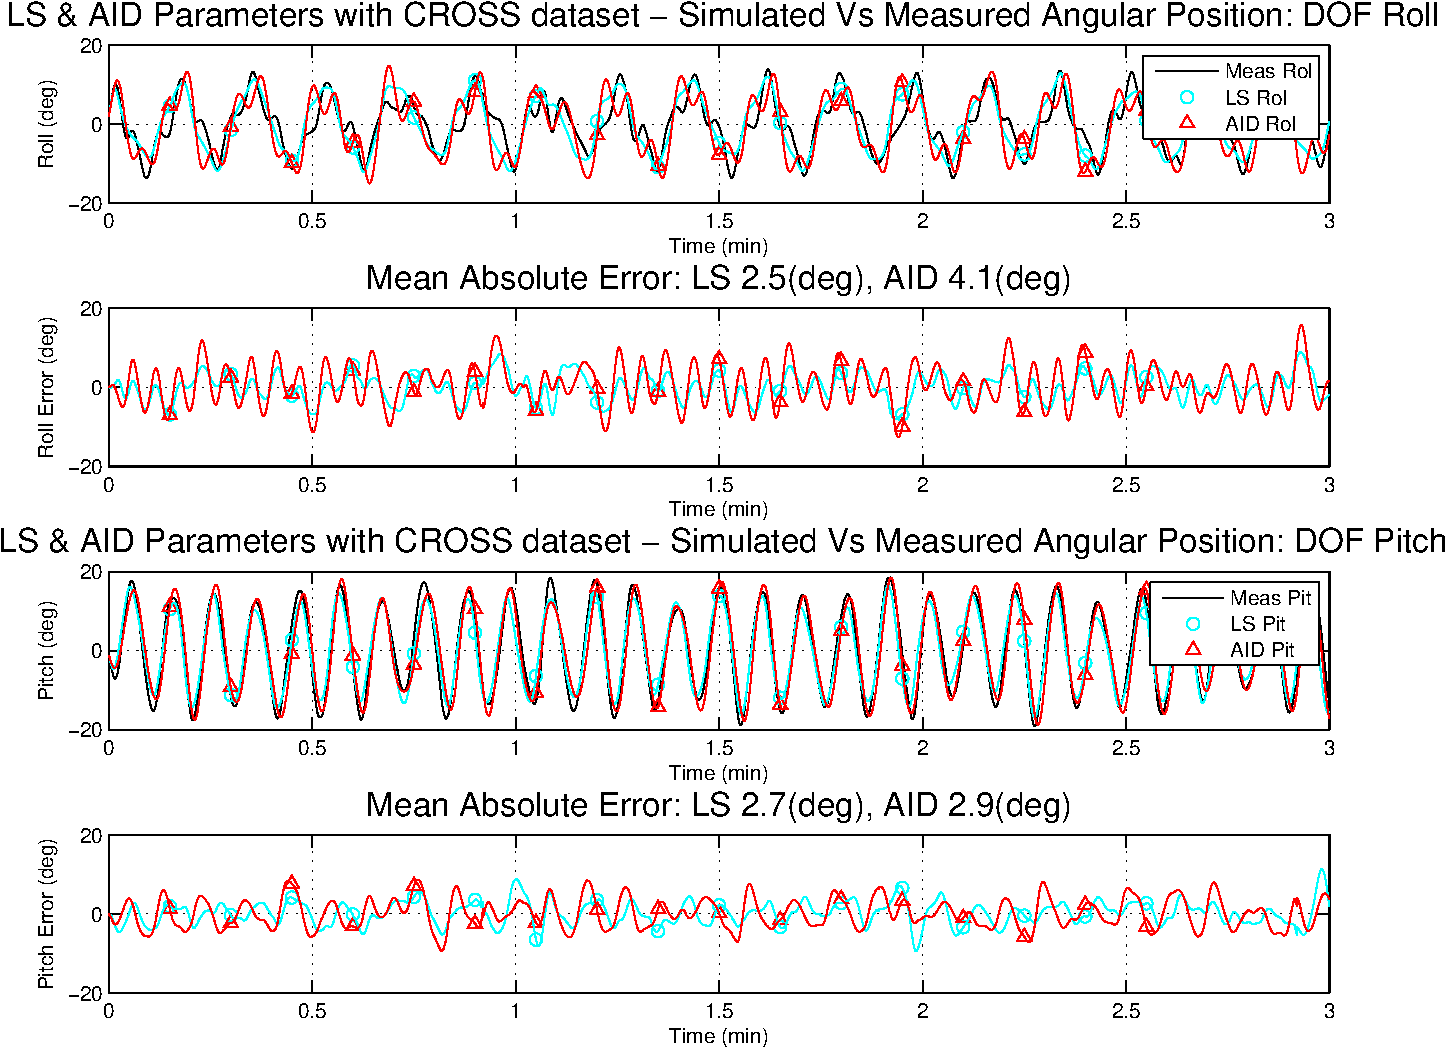
\includegraphics[width=6in]{./chUV_AID/images/crossAID_pos}
  \end{center}
  \caption{Representative data of experimental and simulated
    \ac{JHUROV} angular position for the \ac{CROSS} dataset. In the
    roll and pitch plots, the measured position is plotted together
    with the simulated position from two model simulations. The states
    from a simulation of \ac{AIDPM} are plotted in blue and marked with
    circles. The states from \ac{LSPM} are plotted in red and marked with
    triangles. For each \ac{DOF}, the difference between the measured
    positions from the \ac{CROSS} dataset and the states from each
    model simulation is shown.  For each \ac{DOF},
    the difference between the measured position and simulated
    position is shown. 
%Both models of the
%    \ac{JHUROV} provide a similar capacity to model the system, and
%    both perform better than the simulation using the arbitrary chosen
%    \ac{INITP} shown in Figures \ref{chUV_AID.fig.SO3_INIT_pos} and
%    \ref{chUV_AID.fig.SO3_INIT_vel}.  
}
  \label{chUV_AID.fig.SO3_AID_pos}
\end{figure}
\end{center}

\begin{center}
\begin{figure}[htbp]
  \begin{center}
    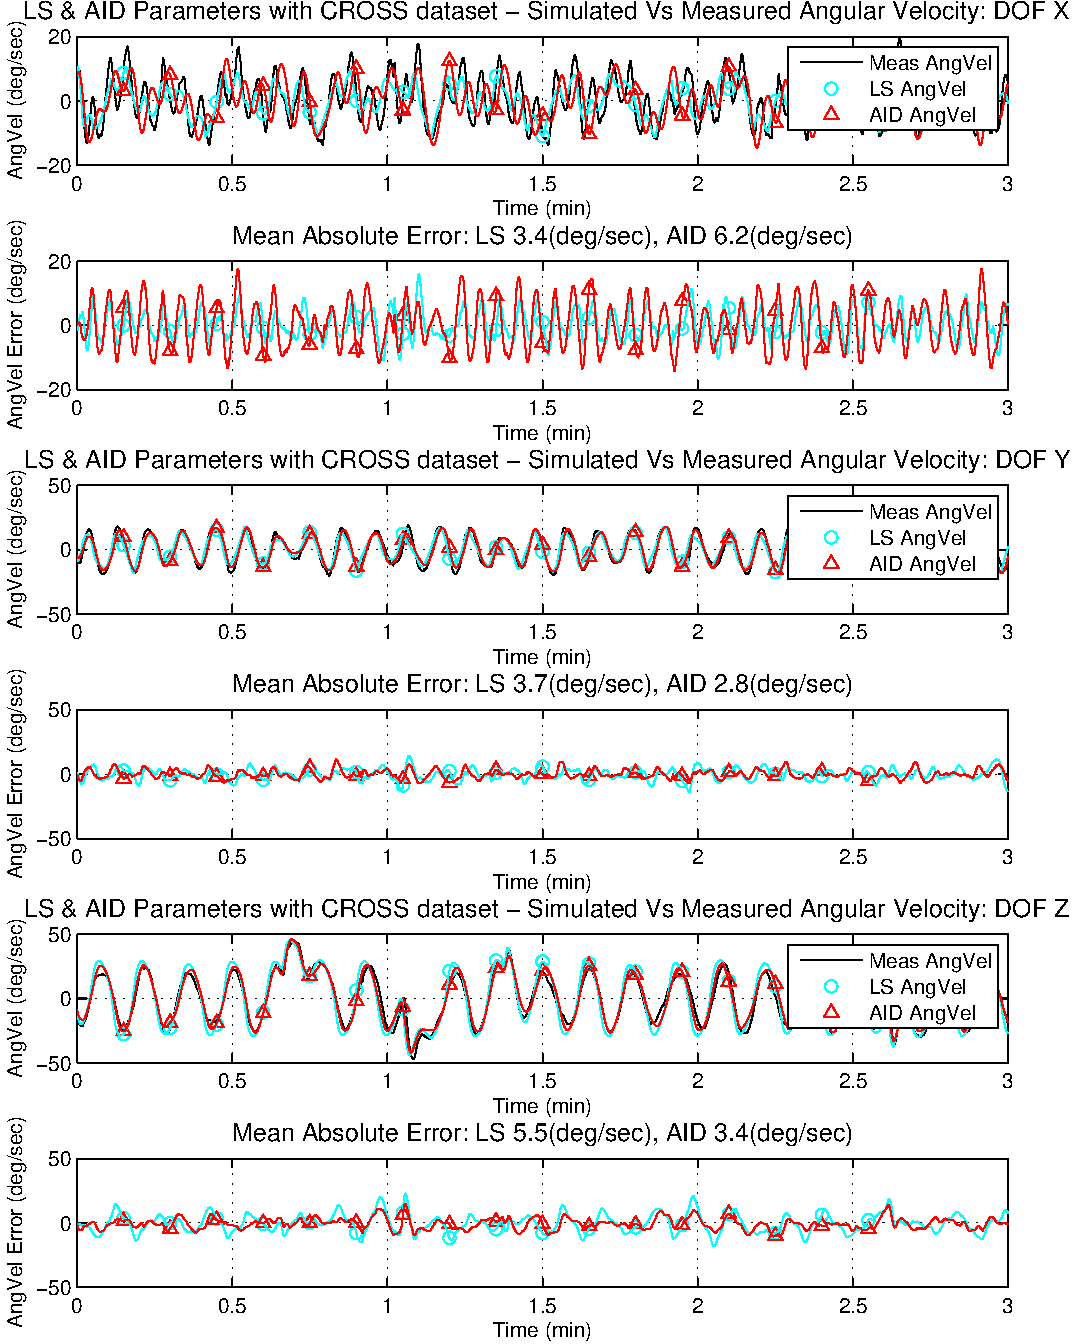
\includegraphics[width=5.5in]{./chUV_AID/images/crossAID_vel}
  \end{center}
  \caption{ Representative data of experimental and simulated \ac{JHUROV}
    angular velocity for the \ac{CROSS} dataset. In the
    individual angular velocity plots, each measured velocity is
    plotted together with velocities from \ac{AIDPM} and \ac{LSPM}
    simulations.  For each \ac{DOF} error plots are also included. See the
    caption of Figure \ref{chUV_AID.fig.SO3_AID_pos} for further information.}
  \label{chUV_AID.fig.SO3_AID_vel}
\end{figure}
\end{center}


% %TM_ENTIRE_UNCOMMENTED_PARAGRAPH_BELOW_ADDED_OK_WITH_LLW?
% Since there is only an emperical basis for using the analytic
% structure (\ref{eq.plantROV}) to model the dynamics of a
% \ac{UV}\cite{martin.thesis}, we are primarily conserned with finding plant
% parameters which match \ac{UV} dynamics over the range of possible
% torque inputs, as there could be a wide range of parameter sets which
% do so.
% %
% Therefore, we focus our analysis on the cross-validation experiment
% which was {\it not} used to identify parameter sets.
% %
% To judge the capacity of a parameter set to model the vehicle, we
% compare states estimated using a parameter set to the states recorded
% during a \ac{JHUROV} experimental run.
% %
% A good model, when used as an open loop observer, will provide
% accurate estimates of the pitch, roll and angular velocities of the
% vehicle when the vehicle's initial state and input torque history are
% used.
% %TM_COULD_ADD_THE_SENTENCE Because of the presence of a buoyancy
% %torque and the large effect of drag on \ac{UV} vehicle operation, the open
% %loop observer estimates can stay near the experimentially recorded
% %states even in the presence of moderate unmodeled exogenious torques. 
% %
% To create the open loop observer estimates \ac{UV} plant models
% (\ref{eq.plantROV}), one for each parameter set, were simulated using a 
% fourth order Runge Kutta numerical differential equation solver.  
% %
% The initial state provided to each simulation was that of the \ac{JHUROV}
% recorded at the start of the experiment, and the input torques used
% where those recorded by the \ac{JHUROV} control system during the
% duration of each experiment.
% %
% We report the mean absolute error (MAE) between each parameter set's
% simulated plant model and the corresponding expermentially observed
% plant states in Table \ref{chUV_AID.tb.SO3_MAE}.

%------------------------OLD_WORDS----------------------------------
% For comparative purposes we consider the differences between the
% values of states measured for \ac{JHUROV} and numerical simulations of
% the \ac{UV} plant model (\ref{eq.plantROV}) using one of the
% parameter sets in Table \ref{tb.paramSets}.
% %
% To simulate the \ac{JHUROV}'s trajectory for a given parameter set, a
% fourth order Runge Kutta numerical differential equation solver was
% used.
% % NEW WORDS
% Both the vehicle and the vehicle model have energy dissipation, an
% attractive equibium point in pitch and an attractive equibium point in
% roll. 
% %
% Because of these system traits, the effects of all previous
% events on the current roll, pitch, and angular velocities will lessen
% the further back in time an event occured. 
% %
% The more damping in a \ac{DOF}, the higher the energy dissipation, and the
% quicker previous events are forgotten.
% %
% If a perfect \ac{JHUROV} model and the \ac{JHUROV} itself are
% provided the same external torque signal, the states of both will
% match for all time.  
% %
% Differences in state which arise could be caused
% by several factors including noise (unmodeled external torques),
% mismatched parameter selection, or flawed model structure
% (\ref{eq.plantROV}).  
% %
% A single event for any of these factors could
% cause a nonzero error state.  
% %
% But since both the expermental and simulated \ac{JHUROV} are being driven
% by the same external torque, the interval of time over which a
% particular event can cause the roll, pitch, or angular velocity errors
% is finite.
% %
% Since modeling errors should be regularly causing differences in
% errors in state,  judging the typical error between the experimental
% and simulated \ac{JHUROV} states should allow us to characterize relative
% performance of each model.
% %
% Thus for pitch, roll, and each angular velocity \ac{DOF} we present plots
% of state, plots of error, and values of mean absolute error (MAE) to
% characterize the relative performance of each model.



\subsection{Analysis of Experimental Results}

Compare the state estimate capacity of \ac{INITPM} in Figures
\ref{chUV_AID.fig.SO3_INIT_pos} and \ref{chUV_AID.fig.SO3_INIT_vel} to
the state estimate capacity of \ac{AIDPM} and \ac{LSPM} Figures
\ref{chUV_AID.fig.SO3_AID_pos} and \ref{chUV_AID.fig.SO3_AID_vel}.
Clearly the simulated plant model's capacity to match experimentally
observed plant performance is dependent on the model's plant
parameters.
%
Comparing the states produced by simulating \ac{AIDPM} and \ac{LSPM}
with those from \ac{INITPM} (a model which uses the arbitrarily chosen
\ac{INITP} parameter set), we see that both experimentally identified
models are better at matching experimentally observed dynamic plant
behavior.
%
Table \ref{chUV_AID.tb.SO3_MAE} confirms that the \ac{AIDPM} and
\ac{LSPM} are better than the \ac{INITPM} at modeling \ac{JHUROV}
performance.
%
In the case of both the \ac{IDDAT} and \ac{CROSS} datasets, the
performance of the \ac{AIDPM} and \ac{LSPM} were similar, i.e.  for
some \ac{DOF} the \ac{AIDPM} states were on average closer to the
experimentally measured state values (as shown by smaller \ac{MAE}
values) and for other \ac{DOF} the \ac{LSPM} states were on average
closer to the experimentally measured values.
%
Figures \ref{chUV_AID.fig.SO3_AID_pos} and
\ref{chUV_AID.fig.SO3_AID_vel} show the dynamic behavior of the two
identified models match the experimentally observed \ac{JHUROV}
performance, though the data in Figure \ref{chUV_AID.fig.SO3_AID_pos}
suggests that the \ac{LSPM} is slightly better at matching the
\ac{JHUROV}'s roll and pitch states.
%
For some \ac{AIDPM} and \ac{LSPM} \acp{DOF}, each model's capacity to
match measured states from the \ac{CROSS} dataset is worse
than their capacity to match states from the \ac{IDDAT} dataset;
%  
in Table \ref{chUV_AID.tb.SO3_MAE} \ac{CROSS} \ac{MAE} values can be
up to 60\% larger that the \ac{IDDAT} \ac{MAE} values for the
equivalent \ac{DOF} and \ac{UV} model.  
%
However, the representative sample of data plotted in Figures
\ref{chUV_AID.fig.SO3_AID_pos} and \ref{chUV_AID.fig.SO3_AID_vel}
indicate that both \ac{AIDPM} and \ac{LSPM} capture the character
character of \ac{JHUROV} performance during cross-validation.


From Figures \ref{chUV_AID.fig.SO3_AID_pos} and
\ref{chUV_AID.fig.SO3_AID_vel} note that roll (motion about the
x-axis) and the x-axis angular velocity have a more complex motion
than the other \ac{DOF}.  
%
This is due to the coupling between the
\ac{DOF}; for the \ac{JHUROV} we have observed that when considering
angular motion about the x, y, and z axes, x-axis motion is the most
sensitive to angular motions about the other axes.  
%
Figures \ref{chUV_AID.fig.SO3_AID_pos}, \ref{chUV_AID.fig.SO3_AID_vel},
and Table \ref{chUV_AID.tb.SO3_MAE} show that angular motion about the
x-axis are the motions least accurately modeled by the \ac{AIDPM}.
%
There are several factors we feel contribute to these larger errors.
%
The first is that both thrusters used to achieve torque about the
x-axis are positioned within the frame of the vehicle whereas all
other thrusters are outside the frame of the vehicle.
%
The internal structures of the vehicle may impede the flow path of
these thrusters and, in consequence, degrade their performance.
%
Additionally, vehicle rotation about the x-axis is the \ac{DOF} with
the least damping and least control authority.
% This light
% damping, and therefore lower energy dissipation, will result in an
% underdamped response in the x-\ac{DOF} error dynamics.
%TM_LLW_LIKE_PREV_SENTENCE_REWRITE?
Thus the lower energy dissipation for rotational motion about the
x-axis could lead to higher \ac{MAE} values for this \ac{DOF}.

%experimental.tex
\section{Experimental Evaluation: 6-\acs{DOF} \acs{UV} \acs{AID}}
\label{chUV_AID.sec.UVSE3exp}

This Section reports a comparative experimental evaluation of \ac{AID}
and \ac{LS} for the estimation of plant parameters for the
dynamics of a 6-\ac{DOF} \ac{UV}.
% 
We employed the Johns Hopkins University Hydrodynamic Test Facility to
evaluate each parameter identification method's capacity to identify
parameter sets which accurately model \ac{UV} dynamics.
%
The error between the predicted model performance and the
experimentally observed performance is reported as the \ac{MAE}
between the simulated plant roll, pitch, and velocity and the actual
experimental plant roll, pitch, and velocity.
%
Appendices \ref{appenJHUHTF.sec.hydrolab} and \ref{appenJHUHTF.sec.paramEvalMethod}
provide further details about our experimental setup and parameter
evaluation method.


During an experiment, each of the six \ac{JHUROV} \acl{DOF} were
independently excited with either closed-loop control or open-loop
sinusoidal commands. For those \ac{DOF} using closed-loop control, a
sinusoidal reference trajectory was specified to the \ac{JHUROV}
control system. The reference signals for both experiments are given
in Table \ref{chUV_AID.tb.UVSE3expStat}.



\begin{table}[htbp]
\ssp
\caption{Input Specifications for 6-\ac{DOF} \ac{UV} Parameter
  Identification Experiments}  
\begin{center}
\begin{tabular}{cccc}
 \multicolumn{2}{c}{Experiment} & \ac{IDDAT}& \ac{CROSS} \\
\hline
\multicolumn{2}{c}{Experiment Purpose}  & Parameter      &  Parameter \\
              &                         & Identification &  Cross-Validation \\
\hline
\multicolumn{2}{c}{Experiment Run Time} &   31.9 min     &   34.8 min    \\ 
\hline
\ac{DOF}      & {\it Excitation Type} & \multicolumn{2}{c}{\it Closed Loop Trajectory-Tracking} \\
world x  &  Cos Frequency  & 0.185 rad/sec & 0.242 rad/sec \\ 
         &  Cos Amplitude  &    0.60 m     &     0.60 m    \\ 
\hline
\ac{DOF}      & {\it Excitation Type} & \multicolumn{2}{c}{\it Closed Loop Trajectory-Tracking} \\
world y  &  Cos Frequency  & 0.286 rad/sec & 0.210 rad/sec \\ 
         &  Cos Amplitude  &    0.60 m     &     0.60 m    \\ 
\hline
\ac{DOF}      & {\it Excitation Type} & \multicolumn{2}{c}{\it Closed Loop Trajectory-Tracking} \\
world z  &  Cos Frequency  & 0.242 rad/sec & 0.185 rad/sec \\ 
         &  Cos Amplitude  &    0.50 m     &     0.50 m    \\ 
\hline
Torque   & {\it Excitation Type} & \multicolumn{2}{c}{\it Open Loop Torque Input} \\
about \ac{DOF}&  Cos Frequency  & 0.262 rad/sec & 0.224 rad/sec \\ 
body x   &  Cos Amplitude  &    40 N m    &     40 N m     \\ 
\hline
Torque   & {\it Excitation Type} & \multicolumn{2}{c}{\it Open Loop Torque Input} \\
about \ac{DOF}&  Cos Frequency  & 0.449 rad/sec & 0.331 rad/sec \\ 
body y   &  Cos Amplitude  &    55 N m    &     55 N m     \\ 
\hline
\ac{DOF}      & {\it Excitation Type} & \multicolumn{2}{c}{\it Closed Loop Trajectory-Tracking} \\
heading  &  Cos Frequency  & 0.210 rad/sec & 0.286 rad/sec \\ 
         &  Cos Amplitude  &    45$^\circ$  &   45$^\circ$   \\ 
\hline \end{tabular}
\end{center}
\label{chUV_AID.tb.UVSE3expStat}
\end{table}



\ac{AID} was implemented as a discrete time approximation of the
continuous time algorithm.  
%
%Once every 100ms the most recent state measurements, commanded
%torque, commanded force, parameter estimates, and velocity
%estimates were used to calculate the velocity and parameter
%estimate derivatives
%(\ref{chUV_AID.eq.UV_SE3_Estimator})-(\ref{chUV_AID.eq.UV_SE3_BuoyId}).
%
Euler integration of
(\ref{chUV_AID.eq.UV_SE3_Estimator})-(\ref{chUV_AID.eq.UV_SE3_BuoyId})
for 100ms time steps
provided the time series of parameter and angular velocity
estimates.
%
100ms is one to two orders-of-magnitude smaller than the state signal
variation rates of 1 second or greater observed during quasi-periodic
\ac{JHUROV} operations.
%
The experiments were designed to generate thruster commands varying
slowly enough to admit the use of steady state thruster models.
%
In practice, first-order Euler integration provided performance
similar to the 4th-order integration implemented in simulation.


The \ac{AID} algorithm was initialized with the measured angular
position, measured angular velocity, measured translational velocity,
and \acf{INITP} in Tables \ref{chUV_AID.tb.UVSE3_INIT_massGravParam}
and \ref{chUV_AID.tb.UVSE3_INIT_dragParam}.
%
%Note that the \ac{INITP} was chosen such that each scalar
%parameter was within an order-of-magnitude of the value to be identified.
%
Based on our previous studies with second-order rigid body adaptive
identification algorithms (Sections \ref{chSMS_ID.sec.SO3_AID_Sim} and
\ref{chUV_AID.sec.UVSO3exp}), we chose adaption gains of $a=10$,
$\gamma_1=5000$, $\gamma_2=20000$, $\gamma_3=2000$, and
$\gamma_4=2000$.


\begin{table}[htbp]
\ssp
\caption{\ac{UV} mass and gravitational parameter values used to initialize \ac{AID}.}
\begin{center}
\begin{tabular}{c|c}
Parameter Symbol & \ac{INITP} Values \\ \hline
$\hat{M}(t_0)$ & $ \left[\begin{array}{cccccc} 100.0 & 0 & 0 & 0 & 0 & 0\\ 0 & 100.0 & 0 & 0 & 0 & 0\\ 0 & 0 & 100.0 & 0 & 0 & 0\\ 0 & 0 & 0 & 100.0 & 0 & 0\\ 0 & 0 & 0 & 0 & 100.0 & 0\\ 0 & 0 & 0 & 0 & 0 & 100.0 \end{array}\right] $ \\ 
$\hat{g}(t_0)$ & 0.0 \\ 
$\hat{b}(t_0)$ & $ \left[\begin{array}{c} 0\\ 0\\ 100.0 \end{array}\right] $ \\ 
\end{tabular}
\end{center}
\label{chUV_AID.tb.UVSE3_INIT_massGravParam}
\end{table}


\begin{table}[htbp]
\ssp
\caption{The \ac{UV} drag parameter values used to initialize \ac{AID}.}
\begin{center}
\begin{tabular}{c|c}
Parameter Symbol & \ac{INITP} Values \\ \hline
$\hat{D}_1(t_0)$ & $ \left[\begin{array}{cccccc} -100.0 & 0 & 0 & 0 & 0 & 0\\ 0 & -100.0 & 0 & 0 & 0 & 0\\ 0 & 0 & -100.0 & 0 & 0 & 0\\ 0 & 0 & 0 & -100.0 & 0 & 0\\ 0 & 0 & 0 & 0 & -100.0 & 0\\ 0 & 0 & 0 & 0 & 0 & -100.0 \end{array}\right] $ \\ 
$\hat{D}_2(t_0)$ & $ \left[\begin{array}{cccccc} -100.0 & 0 & 0 & 0 & 0 & 0\\ 0 & -100.0 & 0 & 0 & 0 & 0\\ 0 & 0 & -100.0 & 0 & 0 & 0\\ 0 & 0 & 0 & -100.0 & 0 & 0\\ 0 & 0 & 0 & 0 & -100.0 & 0\\ 0 & 0 & 0 & 0 & 0 & -100.0 \end{array}\right] $ \\ 
$\hat{D}_3(t_0)$ & $ \left[\begin{array}{cccccc} -100.0 & 0 & 0 & 0 & 0 & 0\\ 0 & -100.0 & 0 & 0 & 0 & 0\\ 0 & 0 & -100.0 & 0 & 0 & 0\\ 0 & 0 & 0 & -100.0 & 0 & 0\\ 0 & 0 & 0 & 0 & -100.0 & 0\\ 0 & 0 & 0 & 0 & 0 & -100.0 \end{array}\right] $ \\ 
$\hat{D}_4(t_0)$ & $ \left[\begin{array}{cccccc} -100.0 & 0 & 0 & 0 & 0 & 0\\ 0 & -100.0 & 0 & 0 & 0 & 0\\ 0 & 0 & -100.0 & 0 & 0 & 0\\ 0 & 0 & 0 & -100.0 & 0 & 0\\ 0 & 0 & 0 & 0 & -100.0 & 0\\ 0 & 0 & 0 & 0 & 0 & -100.0 \end{array}\right] $ \\ 
$\hat{D}_5(t_0)$ & $ \left[\begin{array}{cccccc} -100.0 & 0 & 0 & 0 & 0 & 0\\ 0 & -100.0 & 0 & 0 & 0 & 0\\ 0 & 0 & -100.0 & 0 & 0 & 0\\ 0 & 0 & 0 & -100.0 & 0 & 0\\ 0 & 0 & 0 & 0 & -100.0 & 0\\ 0 & 0 & 0 & 0 & 0 & -100.0 \end{array}\right] $ \\ 
$\hat{D}_6(t_0)$ & $ \left[\begin{array}{cccccc} -100.0 & 0 & 0 & 0 & 0 & 0\\ 0 & -100.0 & 0 & 0 & 0 & 0\\ 0 & 0 & -100.0 & 0 & 0 & 0\\ 0 & 0 & 0 & -100.0 & 0 & 0\\ 0 & 0 & 0 & 0 & -100.0 & 0\\ 0 & 0 & 0 & 0 & 0 & -100.0 \end{array}\right] $ \\ 
\end{tabular}
\end{center}
\label{chUV_AID.tb.UVSE3_INIT_dragParam}
\end{table}


\subsection{Experimental Results}%\label{ref.expResults}

\begin{table}[htbp]
\ssp
\caption{The \ac{UV} mass and gravitational parameters identified
  using \ac{AID} and the \ac{IDDAT} dataset.}
\begin{center}
\begin{tabular}{c|c}
Parameter Symbol & \ac{AIDP} Values \\ \hline
$\hat{M}(t_f)$ & $ \left[\begin{array}{cccccc} 996.9 & -6.166 & 9.118 & 53.64 & -76.78 & 111.7\\ -6.166 & 1275.0 & 14.23 & -56.45 & 41.07 & -43.3\\ 9.118 & 14.23 & 1378.0 & -17.57 & 69.42 & 43.95\\ 53.64 & -56.45 & -17.57 & 308.7 & 21.87 & 39.99\\ -76.78 & 41.07 & 69.42 & 21.87 & 322.3 & -48.32\\ 111.7 & -43.3 & 43.95 & 39.99 & -48.32 & 467.4 \end{array}\right] $ \\ 
$\hat{g}(t_f)$ & -21.77 \\ 
$\hat{b}(t_f)$ & $ \left[\begin{array}{c} 5.966\\ -0.9802\\ 342.8 \end{array}\right] $ \\ 
\end{tabular}
\end{center}
\label{chUV_AID.tb.UVSE3_AID_massGravParam}
\end{table}


\begin{table}[htbp]
\ssp
\caption{The \ac{UV} drag parameters identified using \ac{AID} and the
  \ac{IDDAT} data.}
\begin{center}
\begin{tabular}{c|c}
Parameter Symbol & \ac{AIDP} Values \\ \hline
$\hat{D}_1(t_f)$ & $ \left[\begin{array}{cccccc} -466.7 & 4.902 & -14.54 & -19.92 & -0.3734 & -3.236\\ 71.43 & -331.6 & -27.36 & 119.8 & -13.05 & 12.08\\ -67.64 & -1.584 & -528.8 & -11.23 & 42.6 & -22.18\\ 0.03723 & -12.6 & 97.29 & -270.7 & 19.31 & -56.57\\ 17.39 & -14.41 & -47.56 & -19.17 & -51.29 & 6.865\\ -36.24 & 5.508 & -3.391 & 44.59 & -13.47 & -155.7 \end{array}\right] $ \\ 
$\hat{D}_2(t_f)$ & $ \left[\begin{array}{cccccc} -342.9 & 15.59 & 35.52 & -19.45 & -30.78 & -27.73\\ -16.96 & -618.6 & 68.14 & 107.7 & -37.52 & 42.93\\ 7.135 & 19.27 & -578.9 & 19.15 & 49.08 & -21.97\\ -11.15 & 49.91 & 69.85 & -279.2 & 30.13 & -19.8\\ 52.72 & -63.28 & -11.81 & -22.2 & -42.57 & 38.04\\ -31.44 & 43.94 & -40.48 & 77.72 & -16.38 & -150.4 \end{array}\right] $ \\ 
$\hat{D}_3(t_f)$ & $ \left[\begin{array}{cccccc} -373.0 & 9.072 & 43.92 & -9.852 & -26.69 & 7.863\\ -12.09 & -466.7 & 6.452 & 138.2 & -11.46 & 67.43\\ -31.76 & 52.37 & -685.6 & -1.646 & 20.42 & -2.191\\ -21.4 & 3.283 & 146.3 & -261.8 & 32.96 & -33.43\\ 4.241 & -32.42 & -17.53 & -30.22 & -56.54 & -11.55\\ -45.66 & 24.02 & -38.2 & 40.72 & -28.91 & -241.1 \end{array}\right] $ \\ 
$\hat{D}_4(t_f)$ & $ \left[\begin{array}{cccccc} -292.8 & -10.59 & 35.93 & -8.17 & -18.11 & -25.44\\ 4.436 & -342.0 & 13.63 & 190.4 & -3.024 & 45.74\\ 9.531 & -6.416 & -362.0 & -19.08 & 23.41 & -14.81\\ 2.579 & 32.18 & 62.65 & -207.2 & 16.85 & 2.63\\ 4.186 & -6.082 & -7.507 & -22.97 & -73.4 & 5.957\\ 3.196 & 20.58 & 1.016 & 62.8 & -19.93 & -142.3 \end{array}\right] $ \\ 
$\hat{D}_5(t_f)$ & $ \left[\begin{array}{cccccc} -212.3 & -16.1 & 7.133 & -15.9 & -21.23 & -4.932\\ 19.71 & -242.1 & -6.173 & 44.77 & -7.459 & 19.94\\ -9.7 & -17.81 & -248.4 & 0.08174 & 32.39 & -5.403\\ -2.604 & 11.03 & 39.88 & -162.8 & 24.41 & -9.847\\ 4.528 & -3.59 & -16.11 & -10.59 & -66.71 & 17.56\\ -11.06 & -4.563 & 0.2745 & 19.88 & -14.07 & -148.7 \end{array}\right] $ \\ 
$\hat{D}_6(t_f)$ & $ \left[\begin{array}{cccccc} -398.9 & -8.592 & -25.27 & -11.01 & -43.3 & -25.29\\ -53.06 & -602.1 & 24.9 & 133.0 & -28.92 & 70.24\\ 4.612 & -16.02 & -582.0 & -0.02913 & 77.21 & -53.36\\ -3.501 & 13.71 & 115.5 & -283.3 & 25.63 & -153.0\\ 11.5 & -44.13 & -35.11 & -25.37 & -41.52 & -18.43\\ -57.68 & 33.12 & -49.59 & 76.05 & -17.43 & -109.2 \end{array}\right] $ \\ 
\end{tabular}
\end{center}
\label{chUV_AID.tb.UVSE3_AID_dragParam}
\end{table}



\begin{table}[htbp]
\ssp
\caption{The \ac{UV} mass and gravitational parameters identified
  using \ac{LS} and the \ac{IDDAT} dataset.}
\begin{center}
\begin{tabular}{c|c}
Parameter Symbol & \ac{LSP} Values \\ \hline
$\hat{M}(t_f)$ & $ \left[\begin{array}{cccccc} 446.7 & 13.29 & 35.18 & 20.74 & -27.2 & 37.66\\ 13.29 & 669.5 & -0.2402 & -14.65 & 2.878 & -21.9\\ 35.18 & -0.2402 & 896.2 & -16.36 & 11.14 & 35.23\\ 20.74 & -14.65 & -16.36 & 39.53 & -7.008 & 17.43\\ -27.2 & 2.878 & 11.14 & -7.008 & 65.47 & -2.574\\ 37.66 & -21.9 & 35.23 & 17.43 & -2.574 & 116.8 \end{array}\right] $ \\ 
$\hat{g}(t_f)$ & -19.7 \\ 
$\hat{b}(t_f)$ & $ \left[\begin{array}{c} 0.7842\\ 6.807\\ 279.8 \end{array}\right] $ \\ 
\end{tabular}
\end{center}
\label{chUV_AID.tb.UVSE3_LS_massGravParam}
\end{table}


\begin{table}[htbp]
\ssp
\caption{The \ac{UV} drag parameters identified using \ac{LS} and the
  \ac{IDDAT} dataset.}
\begin{center}
\begin{tabular}{c|c}
Parameter Symbol & \ac{LSP} Values \\ \hline
$\hat{D}_1(t_f)$ & $ \left[\begin{array}{cccccc} -640.7 & 29.14 & -77.14 & -206.0 & 399.7 & -57.4\\ 426.7 & -146.6 & -191.1 & -53.18 & 310.4 & -242.6\\ 50.05 & -65.4 & -1078.0 & 216.5 & 32.88 & -108.7\\ -2.037 & 35.94 & 4.818 & -557.7 & -19.11 & 58.69\\ 60.09 & 65.24 & -2.878 & 78.19 & -108.7 & 74.52\\ -32.74 & 15.27 & -19.89 & -77.99 & 81.52 & -82.61 \end{array}\right] $ \\ 
$\hat{D}_2(t_f)$ & $ \left[\begin{array}{cccccc} -416.7 & -54.12 & 88.38 & -53.97 & -79.78 & -63.98\\ -20.42 & -575.1 & 101.8 & -75.27 & -260.0 & 67.67\\ -25.36 & -75.01 & -979.1 & 429.8 & -130.5 & -45.88\\ -37.62 & 69.31 & 0.004228 & -318.2 & 73.01 & 16.12\\ 52.75 & -31.51 & -40.18 & -32.51 & -183.8 & 10.49\\ -62.16 & -15.68 & -89.55 & 33.62 & 243.3 & -220.9 \end{array}\right] $ \\ 
$\hat{D}_3(t_f)$ & $ \left[\begin{array}{cccccc} -894.2 & 293.0 & 42.96 & -203.4 & -424.3 & 15.49\\ -115.2 & -1247.0 & -215.0 & 164.9 & 283.9 & 131.6\\ -120.7 & 165.4 & -901.3 & 72.91 & -150.7 & 168.2\\ -25.58 & 84.36 & 195.6 & -318.2 & -40.94 & 26.2\\ 145.6 & -164.2 & -46.79 & 73.39 & -321.2 & 27.31\\ -115.2 & 164.7 & -143.7 & -67.74 & -72.01 & -514.8 \end{array}\right] $ \\ 
$\hat{D}_4(t_f)$ & $ \left[\begin{array}{cccccc} -22.32 & -55.78 & 266.5 & 233.5 & -737.6 & 258.0\\ -445.6 & -242.8 & 463.0 & 1680.0 & 255.3 & -128.4\\ 61.74 & -83.5 & -454.2 & -943.5 & -53.48 & -144.2\\ 45.38 & 149.0 & -167.4 & 235.8 & -10.58 & 40.72\\ 89.95 & -16.57 & -114.2 & -32.4 & -58.5 & -80.68\\ -39.36 & -14.35 & 135.3 & 278.7 & -508.8 & -114.7 \end{array}\right] $ \\ 
$\hat{D}_5(t_f)$ & $ \left[\begin{array}{cccccc} -541.9 & -201.2 & -218.5 & -4.108 & -1155.0 & 338.4\\ 802.6 & -1098.0 & -648.5 & -353.1 & -46.14 & -232.1\\ 123.8 & -116.6 & -1045.0 & 209.3 & -203.8 & -111.9\\ -81.21 & 59.62 & 6.686 & -450.4 & 90.86 & 44.2\\ 11.35 & 45.01 & 96.38 & -126.6 & 216.3 & 41.87\\ -41.39 & -1.279 & 223.2 & -8.406 & -221.2 & -42.09 \end{array}\right] $ \\ 
$\hat{D}_6(t_f)$ & $ \left[\begin{array}{cccccc} -310.2 & 98.97 & -39.83 & 86.85 & 22.8 & -142.3\\ -172.0 & -730.8 & 113.5 & 166.2 & -560.2 & 266.3\\ 1.31 & -43.02 & -536.0 & 166.4 & 370.4 & 68.14\\ -22.85 & 1.085 & 16.88 & -247.2 & -57.23 & -76.39\\ -28.74 & -68.49 & -109.2 & 28.06 & -310.4 & 17.32\\ -155.9 & 21.63 & -77.06 & -27.19 & 40.62 & -24.28 \end{array}\right] $ \\ 
\end{tabular}
\end{center}
\label{chUV_AID.tb.UVSE3_LS_dragParam}
\end{table}


The \ac{IDDAT} dataset was used to identify plant parameters of the
6-\ac{DOF} plant model (\ref{chModels.eq.UVSE3plant}) with both the
adaptive identification and least squares algorithms.
%
\Cref{chUV_AID.tb.UVSE3_AID_massGravParam,chUV_AID.tb.UVSE3_AID_dragParam}
report the \acf{AIDP} estimated using  6-\ac{DOF} \ac{UV} \ac{AID} (as
per Section \ref{chUV_AID.sec.UV_SE3_AID}).
%
\Cref{chUV_AID.tb.UVSE3_LS_massGravParam,chUV_AID.tb.UVSE3_LS_dragParam}
report the \acf{LSP}  estimated using 6-\ac{DOF} \ac{UV} \ac{LS} (as
per Section \ref{chUV_AID.sec.leastSquares}).
%
The parameter sets \ac{AIDP}, \ac{LSP}, and \ac{INITP} were used as
 parameter sets for three 6-\ac{DOF} \ac{UV} models;
the \acf{AIDPM}, the \acf{LSPM}, and the \acf{INITPM}.


Using the force and torque inputs from the \ac{CROSS} dataset,
\Cref{chUV_AID.fig.SE3_crossPos,chUV_AID.fig.SE3_crossBodVel,chUV_AID.fig.SE3_crossAngVel}
compare the states from simulations of \ac{AIDPM},
\ac{LSPM}, and \ac{INITPM} to the measured \ac{JHUROV} states from
the \ac{CROSS} dataset.
%
Each of these Figures display three minute subsets of 30 minutes of
state data generated by driving simulations of \ac{AIDPM},
\ac{LSPM}, and \ac{INITPM} using the torque data from the \ac{CROSS}
dataset.
%
Similar simulations of \ac{AIDPM}, \ac{LSPM}, and \ac{INITPM} were
created using the force and torque commands from the \ac{IDDAT} dataset.
%
\Cref{chUV_AID.tb.SE3_pos_MAE,chUV_AID.tb.SE3_vel_MAE} summarize the \ac{MAE} between
measured and simulated vehicle state for each experimental dataset,
6-\ac{DOF} \ac{UV} model, 
and open-loop-stable \ac{DOF}.


%changes after matlab generate MAE table:
% 1)split this table into two tables, 
% 2) moved "paramter set" onto two table rows,
% 3)added the over-labels for velocites, 
% 4)changed the first couple words of both captions
% 5)added '0' to numeric values where sigificant figure rules required it
% 6)changed table labels 

\begin{table}[htbp]
\ssp
\caption{\acfp{MAE} between measured and simulated angular position states for  
  all pairs of 6-\ac{DOF} \ac{UV} experiments and 6-\ac{DOF} \ac{UV} models.}
\begin{center}
\begin{tabular}{p{1.75cm}|ccc}
 \ac{UV}    &          &     &      \\
  Model     & Experiment & Rol & Pit  \\ \hline
\ac{AIDPM} & \ac{CROSS} & 2$^\circ$ & 2.1$^\circ$  \\
\ac{LSPM} & \ac{CROSS} & 1.38$^\circ$ & 1.65$^\circ$  \\
\ac{INITPM} & \ac{CROSS} & 9.9$^\circ$ & 15.0$^\circ$  \\
\ac{AIDPM} & \ac{IDDAT} & 1.96$^\circ$ & 2.3$^\circ$  \\
\ac{LSPM} & \ac{IDDAT} & 1.30$^\circ$ & 1.50$^\circ$  \\
\ac{INITPM} & \ac{IDDAT} & 10.0$^\circ$ & 15.2$^\circ$  \\
\end{tabular}
\end{center}
\label{chUV_AID.tb.SE3_pos_MAE}
\end{table}
%

\begin{table}[htbp]
\ssp
\caption{\acfp{MAE} between simulated and measured velocity states for  
  all pairs of 6-\ac{DOF} \ac{UV} experiments and 6-\ac{DOF} \ac{UV} models.}
\begin{center}
\begin{tabular}{p{1.5cm}|ccccccc}
\ac{UV}  &  & \multicolumn{3}{c}{Translational Velocity} & \multicolumn{3}{c}{Angular Velocity} \\
 Model & Exp  & BodVelX & BodVelY & BodVelZ & AngVelX & AngVelY & AngVelZ \\ \hline
\ac{AIDPM} & \ac{CROSS}  & 0.062m/s & 0.058m/s & 0.037m/s & 1.39$^\circ$/s & 1.35$^\circ$/s & 5.0$^\circ$/s \\
\ac{LSPM} & \ac{CROSS}  & 0.050m/s & 0.052m/s & 0.024m/s & 1.38$^\circ$/s & 1.39$^\circ$/s & 6.3$^\circ$/s \\
\ac{INITPM} & \ac{CROSS}  & 0.165m/s & 0.26m/s & 0.25m/s & 5.1$^\circ$/s & 3.3$^\circ$/s & 3.9$^\circ$/s \\
\ac{AIDPM} & \ac{IDDAT}  & 0.061m/s & 0.06m/s & 0.039m/s & 1.62$^\circ$/s & 1.43$^\circ$/s & 3.4$^\circ$/s \\
\ac{LSPM} & \ac{IDDAT}  & 0.045m/s & 0.048m/s & 0.026m/s & 1.58$^\circ$/s & 1.25$^\circ$/s & 4.1$^\circ$/s \\
\ac{INITPM} & \ac{IDDAT}  & 0.156m/s & 0.27m/s & 0.29m/s & 6.8$^\circ$/s & 3.4$^\circ$/s & 3.8$^\circ$/s \\
\end{tabular}
\end{center}
\label{chUV_AID.tb.SE3_vel_MAE}
\end{table}




\begin{center}
\begin{figure}[htbp]
  \begin{center}
    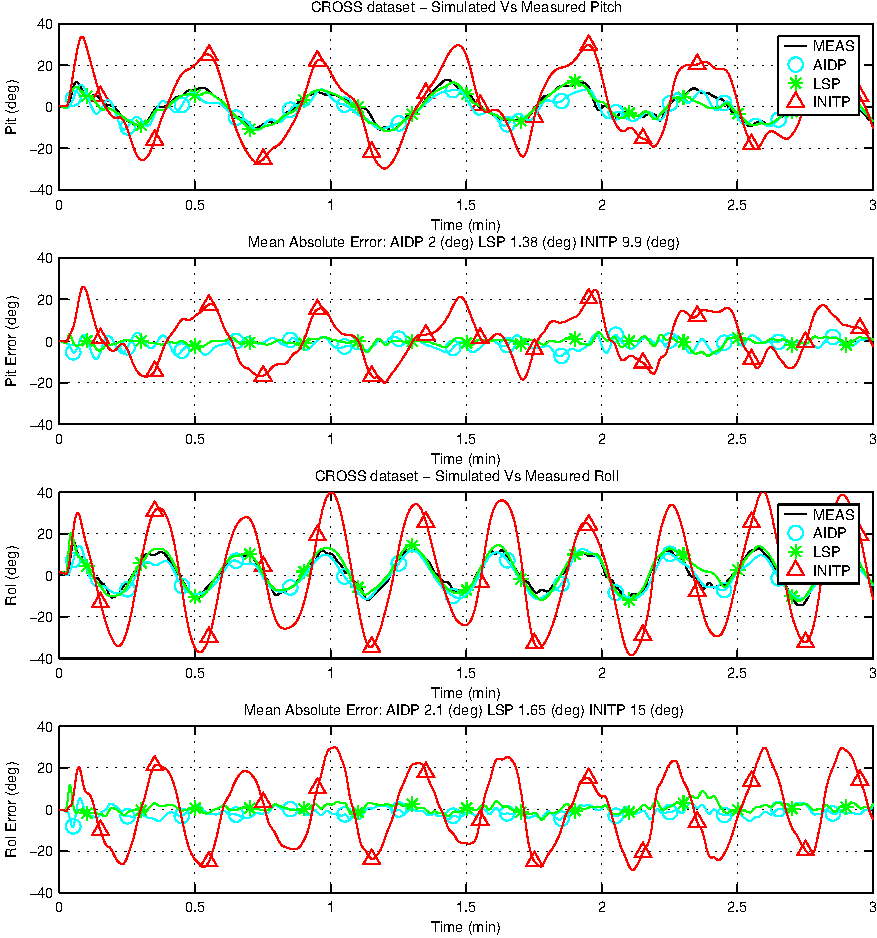
\includegraphics[width=6in]{./chUV_AID/images/SE3_crossPos}
  \end{center}
  \caption{ Representative data of experimental and simulated
    \ac{JHUROV} states for the \ac{CROSS} dataset. In the pitch and
    roll plots, the measured state is plotted together with the
    simulation state from three model simulations. The states from
    \ac{AIDPM} are plotted in blue and marked with circles.  The
    states from \ac{LSPM} are plotted in green and marked with stars.
    The states from \ac{INITPM} are plotted in red and marked with
    triangles.  For each \ac{DOF}, the error between the measured
    positions and their estimates is shown.  }
  \label{chUV_AID.fig.SE3_crossPos}
\end{figure}
\end{center}


\begin{center}
\begin{figure}[htbp]
  \begin{center}
    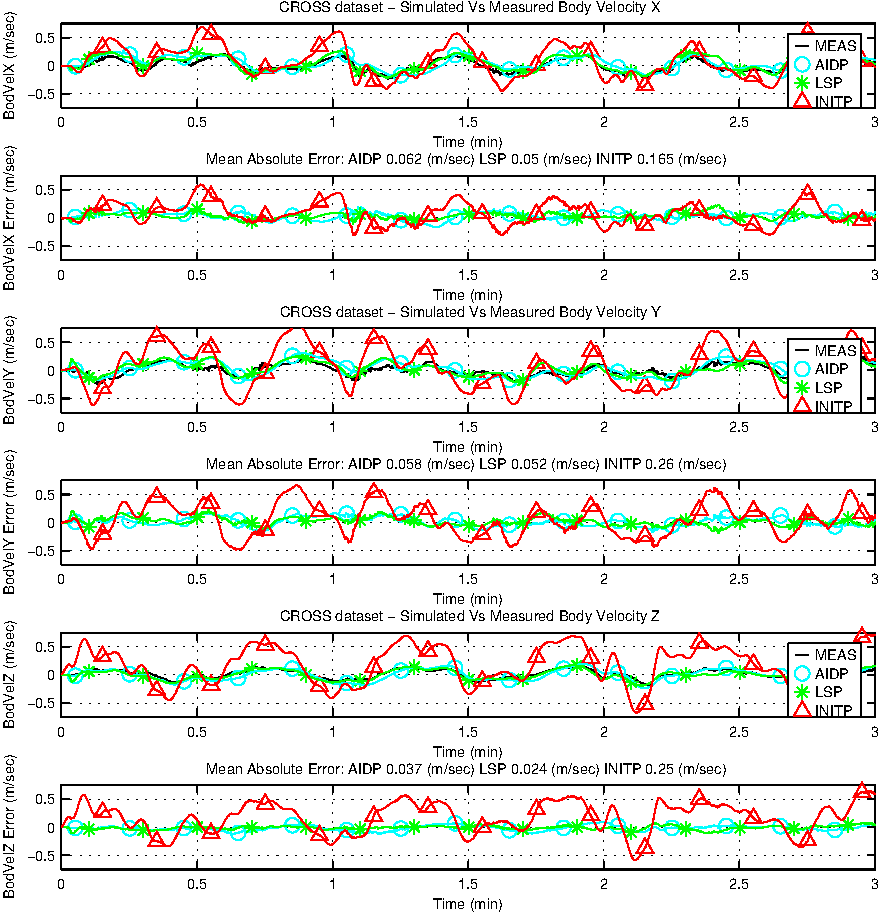
\includegraphics[width=6in]{./chUV_AID/images/SE3_crossBodVel}
  \end{center}
  \caption{
    Representative data of experimental and simulated
    \ac{JHUROV} states for the \ac{CROSS} dataset. In the x, y and z
    body velocity, the measured state is plotted together with the
    simulation state from three model simulations. The states from
    \ac{AIDPM} are plotted in blue and marked with circles.  The
    states from \ac{LSPM} are plotted in green and marked with stars.
    The states from \ac{INITPM} are plotted in red and marked with
    triangles.  For each \ac{DOF}, the error between the measured
    positions and their estimates is shown. 
  }
  \label{chUV_AID.fig.SE3_crossBodVel}
\end{figure}
\end{center}



\begin{center}
\begin{figure}[htbp]
  \begin{center}
    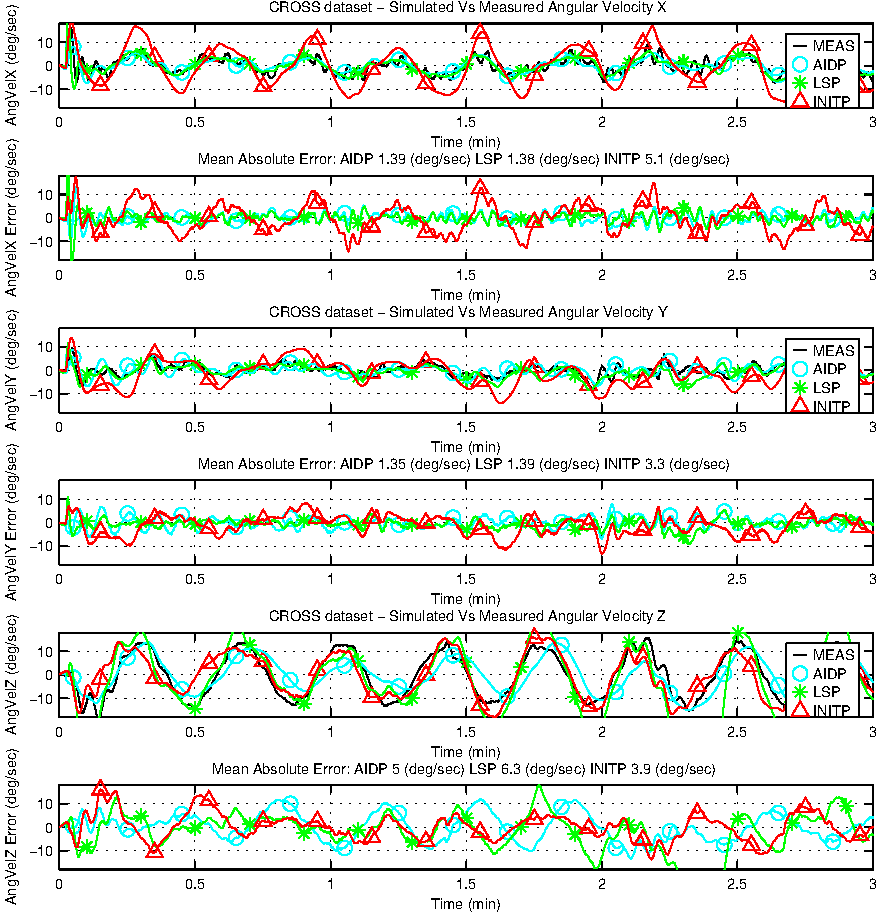
\includegraphics[width=6in]{./chUV_AID/images/SE3_crossAngVel}
  \end{center}
  \caption{ Representative data of experimental and simulated
    \ac{JHUROV} states for the \ac{CROSS} dataset. In the x, y and z
    angular velocity plots, the measured state is plotted together
    with the simulation state from three model simulations. The states
    from \ac{AIDPM} are plotted in blue and marked with circles.  The
    states from \ac{LSPM} are plotted in green and marked with stars.
    The states from \ac{INITPM} are plotted in red and marked with
    triangles.  For each \ac{DOF}, the error between the measured
    positions and their estimates is shown.}
  \label{chUV_AID.fig.SE3_crossAngVel}
\end{figure}
\end{center}


\subsection{Analysis of Experimental Results}


\Cref{chUV_AID.fig.SE3_crossPos,chUV_AID.fig.SE3_crossBodVel,chUV_AID.fig.SE3_crossAngVel}
reveal that the ability of a simulated plant model to match
experimentally observed plant performance is dependent on the model's
plant parameters.
%
Comparing the states produced by simulating \ac{AIDPM} and \ac{LSPM}
with those from \ac{INITPM} (a model which uses the arbitrarily chosen
\ac{INITP} parameter set), we see that both experimentally identified
models are better at matching experimentally observed dynamic plant
behavior.
%
Tables \ref{chUV_AID.tb.SE3_pos_MAE} and \ref{chUV_AID.tb.SE3_vel_MAE}
confirm that the \ac{AIDPM} and \ac{LSPM} match \ac{JHUROV} performance
better than the \ac{INITPM}.

Tables \ref{chUV_AID.tb.SE3_pos_MAE} and
\ref{chUV_AID.tb.SE3_vel_MAE} suggest that both identified models provide
similar \ac{MAE} values for the \ac{IDDAT} dataset.
%
However, since this experiment was used to identify both models, the
question arises ``How will each model reproduce vehicle performance
for experiments not used for model identification?''  
%
The rest of this discussion addresses this important question, 
focusing on which (if any) of the  identified models are better at matching
\ac{JHUROV} performance in cross-validation (as per Appendix \ref{appenJHUHTF.sec.paramEvalMethod}).
%
\ac{MAE} values from comparing simulated and measured states for the
\ac{CROSS} dataset show that modeling the \ac{JHUROV} using the \acf{LSPM}
is marginally better than modeling the \ac{JHUROV} using the \acf{AIDPM},
as seen in the angular position \acp{MAE} in Table
\ref{chUV_AID.tb.SE3_pos_MAE} and translational velocity \acp{MAE} in
Table \ref{chUV_AID.tb.SE3_vel_MAE}.
%
Both Figure \ref{chUV_AID.fig.SE3_crossAngVel} and Table
\ref{chUV_AID.tb.SE3_vel_MAE} indicate that the \ac{AIDPM} and
\ac{LSPM} provide a similar capacity to estimate the \ac{JHUROV}'s
angular velocity.
%
In
\Cref{chUV_AID.fig.SE3_crossPos,chUV_AID.fig.SE3_crossBodVel,chUV_AID.fig.SE3_crossAngVel}
the \ac{LSPM} and \ac{AIDPM} accurately reproduce the experimentally
observed states, failing only to reproduce the very highest frequency
fluctuations observed experimentally (such as those seen in the x
angular velocity subplots of Figure
\ref{chUV_AID.fig.SE3_crossAngVel}).
%
Taken together
\Cref{chUV_AID.fig.SE3_crossPos,chUV_AID.fig.SE3_crossBodVel,chUV_AID.fig.SE3_crossAngVel}
and \Cref{chUV_AID.tb.SE3_pos_MAE,chUV_AID.tb.SE3_vel_MAE} indicate
that the character of \ac{JHUROV} performance is captured well by both
the \ac{LSPM} and \ac{AIDPM}.



%-------------------------------------------------------------------
% Figure \ref{fig.crossAll} shows that the ability for a simulated model
% plant to match experimentally observed plant performance is dependent
% on the model plant parameters.
% %
% Comparing the AID and LS parameter sets with the arbitrarily chosen
% INIT parameter set, the two experimentally identified parameter sets
% provide much better estimates of the vehicle's states.
% %
% Table \ref{tb.MAE} confirms that the AID and LS parameter sets are
% better than the INIT parameter set at modeling \ac{JHUROV} performance.
% %
% Considering the LS and AID model performance for IDDAT, the LS model
% is better at matching the measured vehicle states.
% %
% However, using the same dataset to both create and evaluate a model
% can be a poor predictor of model performance for other inputs.
% %
% Therefore we have performed the cross-validation experiment CROSS.
% %
% Note that all three models provide similar MAE values for both the
% IDDAT and CROSS datasets, an indication that each model will provide
% similar predictive accuracy across the class of inputs physically
% possible for \ac{JHUROV} operation.


% The cross-validation shows that the LS model is better at matching the
% measured vehicle states than the AID model, especially in the angular
% position and linear velocity \ac{DOF}s.
% %
% Table \ref{tb.MAE} indicates that both models provide a similar
% capacity to estimate the \ac{JHUROV}'s angular velocity, which can be seen
% in the Figure \ref{fig.crossAll} y angular velocity plots.
% %
% Here note the complex trajectory the \ac{JHUROV} is following in angular
% velocity.
% %
% Both the LS and AID models are following the general direction of JHU
% ROV angular accelerations with most of the modeling error coming from
% an inability to model the finer details.
% %
% The example plots for two other \ac{DOF} (roll and body
% velocity z) in Figure \ref{fig.crossAll} show the \ac{JHUROV} following
% simpler trajectories.  
% %
% In the roll and body velocity z \ac{DOF}s the LS and AID models are closely
% following the measured \ac{JHUROV} states.
% %
% However, in both \ac{DOF}, specific times can be seen where the AID model
% states are slightly larger offset from measured states.
% %
% Taken together, Figure \ref{fig.crossAll} and Table \ref{tb.MAE}
% indicate that the LS model is marginally better at matching measured
% vehicle performance, but the character of \ac{JHUROV} performance is well
% captured by both identified models.

\section{Summary}
\label{ch.UV_AID.summary}


This Chapter reported two \acf{AID} algorithms  for the dynamic
estimation of \acf{UV} plant parameters.
% 
The \acl{AID} algorithms require the signals of the plant's velocity,
position, and external inputs force, but it does not require any
specific controller, in contrast to previously reported model-based
adaptive tracking controllers.
% 
Many \acl{UV} systems do not allow for adaptive tracking controllers because
they are under-actuated or have other control constraints.
%
%Section \ref{sec.ROVAID} reported a new adaptive identification
%algorithm which is locally asymptotically stable in the
%velocity errors and locally stable in each parameter error.
%
Sections \ref{chUV_AID.sec.UVSO3exp} and \ref{chUV_AID.sec.UVSE3exp}
report comparative experimental evaluations of the \acl{AID} algorithms.
%
Both the \acl{LSPM} and \acl{AIDPM} were shown to match
closely the experimentally observed \acl{UV} input-output behavior.
%
Future work could address less conservative bounds for the initial
error in the parameter estimates, characterize more
precisely conditions for asymptotic parameter convergence, and compare
the relative strengths and weaknesses of adaptive and least squares
parameter identification methods.



\chapter{Adaptive Model-Based Control of Underwater Vehicles}
\label{chUV_AMBC}
\chaptermark{\acs{UV} Adaptive Model-Based Control}
%\ssp
\acresetall



%\section{INTRODUCTION} \label{sec.intro} 


This Chapter addresses the problem of adaptive model-based trajectory
tracking control of \acp{UV} for dynamic 6-\ac{DOF} motion.
%
The approach employed herein, \ac{AMBC}, estimates plant parameters
during the trajectory-tracking control process.
%
The adaptive controller estimates parameters for a rigid-body plant
such as vehicle mass and added hydrodynamic mass parameters; quadratic
drag parameters; and gravitational force and buoyancy parameters that
arise in the dynamic models of rigid-body \acp{UV}.
%
We report a non-adaptive model-based control algorithm for
trajectory-tracking control of fully-actuated rigid-body underwater
vehicles, its adaptive extension, and mathematical analysis of the
stability of the resulting closed-loop systems.
%
We report a comparative experimental evaluation of \ac{AMBC} and
\ac{PDC} in full scale vehicle trials utilizing the Johns Hopkins
University Hydrodynamic Test Facility and \ac{JHUROV} (Appendix
\ref{appenJHUHTF.sec.hydrolab}).
%
The experimental evaluation shows that \ac{AMBC} provides better
position tracking performance (30\%) and marginally worse velocity
tracking performance (8\%) over \ac{PDC}.
%
To the best of the authors' knowledge, this is the first experimental
comparison of \ac{AMBC} and \ac{PDC} \acp{UV} during simultaneous
motion in all six \ac{DOF}.


This Chapter is in two parts. 
%
Section \ref{chUV_AMBC.sec.theory} reports a non-adaptive \ac{MBC} algorithm and
an \ac{AMBC} algorithm for \acp{UV}.
%
Section \ref{chUV_AMBC.sec.unmodeledActDyn} reports results indicating 
that unmodeled thruster dynamics can destabilize parameter
adaptation and a two-step \ac{AMBC} algorithm which is robust to 
unmodeled thruster dynamics. 


The results from Sections \ref{chUV_AMBC.sec.twoStepMethod} and
\ref{chUV_AMBC.sec.unmodeledActDyn} are reported in a paper submitted
to the 2014 International Conference on Robotics and Automation
\cite{mcfarland.icra2014}.

%----------------------------------------------------------------
%----------------------------------------------------------------

% However 
% %
% %DON'T USE SUCH A COMPLEX SENTENCE STRUCTURE
% Although this paper reports a novel MBAC for \ac{UV}, the
% main objective of this text is presenting practial {\color{red}
%   difficulties} to \ac{UV} \ac{AMBC} and solutions to those {\color{red}
%   difficulties}.
% %
% As such, ...


% %----- somewhere in here---------------
% In this paper we propose using Adaptive Tracking Control algorithm

% from \ref{theo.UV_AMBC} assuming the gravitational parameters ($g$
% and $b$) are known.  In Section \ref{sec.fullAnalysisFailure} we show
% \ac{UV} Full-Parameter \ac{AMBC} fails due to thruster stiction during pitch
% and/or roll actuation.  In Section \ref{sec.twoStepExp} we demonstrate
% experimentially that \ac{UV} Dynamic-Only-Parameter \ac{AMBC} provides
% asmtotically improving trajectory-tracking, a good model of vehicle
% performance.  It is therefore robust to the thruster stiction failure
% mode seen in the Full-Parameter 


% Section ____ presents two experiments where \ac{AMBC} is used to follow a pitch only referece trajectory.  
% %
% The range of motion is changed such that one pitch only reference
% trajectroy requires thrust reversals and the other pitch only
% reference trajectory does not.
% %
% A comparative analysis of the parameter adaption process of these
% single \ac{DOF} experiments shows how a small amount of unmodeled dynamics
% near thrust reversals can cause unstable parameter adaptation.
% %
% Section _____ shows how a straightforward implmentation of the \ac{AMBC}
% presented exhibits unstable parameter adaptation in the presence of
% unmodeled thruster dynamics during thrust reversals.
% %
% Section _____ shows the two-step alogithm provides an \ac{AMBC} which,
% while still in the presence of unmodeled dynamics near thrust
% reversals, still provides improved trajectory-tracking and parameters
% estimats which are physically realistic.

\section{Literature Review}
 
Adaptive controllers for linear plants are
well understood 
\cite{ksn&anu.book}.
%\cite{ksn&anu.book,sastry&bodson.book,astrom.book}.
% 
Adaptive reference trajectory-tracking is well
understood for several types of second-order holonomic nonlinear
plants whose parameters enter linearly into the plant equations of
motion, e.g. robot manipulator arms
\cite{Craig&hsu&sastry.ijrr87,slotine&li.ijrr87,horowitz&sadegh.ijrr90},
 spacecraft \cite{kod.cdc85a,slotine1990},
and  rigid-body rotational plants \cite{Chaturvedi2006}.
% rigid-body rotational plants \cite{Chaturvedi2006}, and general
%mechanical systems \cite{Lain1997}.
%
Comparative experimental evaluations of \ac{AMBC} for robot manipulator
arms have been reported, e.g. \cite{slotine.performance,whitcomb&kod.tra93}.



The structure of the \ac{MBC} algorithm reported herein was
inspired by the proportional derivative tracking control algorithm for
rigid-body motion in free space reported by Bullo and
Murray\cite{bullo1995_SE3_PD}.
%
Our controller can be seen as a specialization of this result for
\ac{UV} control; we use their error coordinate structure with a
fully-coupled lumped-parameter plant model of \ac{UV} dynamics,
(\ref{chModels.eq.UVSE3plant}).
%
Fully-coupled lumped-parameter plant models for \acp{UV} use a finite
set of plant parameters which have been shown empirically to be a good
approximation for the complex dynamics of a rigid-body and
associated fluid-vehicle interaction.
%
Lumped-parameter models of \ac{UV} dynamics are used in previously
reported \ac{MBC} algorithms.
%
In \cite{fossen}, Fossen summarizes lumped-parameter modeling of
\ac{UV} dynamics and \ac{UV} \ac{MBC} using a lumped-parameter
modeling and traditional error coordinates.
%
\cite{smallwood2004JOE} reports and experimentally evaluates 
single \ac{DOF} \ac{UV} \ac{MBC} algorithms for control of the 
x, y, depth, and heading \ac{DOF}.
%
\cite{martinControl_ICRA13} reports and experimentally evaluates a
\ac{UV} \ac{MBC} algorithm assuming a fully-coupled lumped-parameter
model; this comparative experimental evaluation of \ac{MBC} and
\ac{PDC} included reference trajectories requiring simultaneous motion
in all \ac{DOF} and was conducted using the Johns Hopkins University
Hydrodynamic Test Facility (Appendix \ref{appenJHUHTF}).



Previous studies have utilized a lumped-parameter \ac{UV} models in
the development of tracking control algorithms which are robust to
model parameter uncertainty.
%
In \cite{yoerger&slotine.JOE85} a sliding mode controller and
numerical simulations of performance in X, Y, and heading is reported.
%
In \cite{Yuh1990} a discrete time parameter adaptation algorithm is
reported with a numerical simulation study.  
%
In \cite{Fossen1991} the authors report a hybrid (adaptive and
sliding) nonlinear \ac{UV} controller which explicitly handles
multiplicative uncertainty in the input mapping.


Experimental evaluations of \ac{AMBC} algorithms have also been
reported.
%
Yoerger et al. reported the first experimental evaluation of nonlinear
adaptive sliding-mode control on an \ac{UV} \cite{yoerger.icra91}.
%
In \cite{yuhICRA1999} an experimental evaluation of \ac{UV} \ac{AMBC}
performance in the presence of noisy position readings is reported.
%
In \cite{antonelli&sarkar.cst2001} an experimental evaluation of an
\ac{AMBC} is reported for simultaneous motion in the translational
\acp{DOF}.
%
Comparative experimental evaluations of linear controllers,
model-based controllers, and their adaptive extensions for \ac{UV} single
\ac{DOF} motion have been reported \cite{smallwood2004JOE, maalouf2013pd}.
%are the subject of a compartive experimental evaluation using the JHU
%ROV.
%
In \cite{zhao2005experimental} a comparative experimental evaluation
in the presence of a common external disturbance for proportional
integral derivative control, disturbance observer control and the
adaptive extensions of both is reported.
%
%In \cite{} an \ac{AMBC} algorithm for \ac{UV} depth control is
%presented and implemented on a test vehicle.
%
In each of these previously reported experimental evaluations at most
two \ac{DOF} had a non-zero reference velocity at a given moment, and
in all cases at most set-point regulation was reported in the pitch and
roll \ac{DOF}.

\section{ Adaptive Model-Based Tracking Control of Underwater Vehicles}
\label{chUV_AMBC.sec.theory}


Recent advances in enabling technologies for \acp{UV} including {\it in-situ}
sensing, power storage, and communication modalities have enabled the
development of \acp{UV} which can accomplish missions previously thought
impractical or impossible.
%
Many of these missions, such as seafloor surveying and
environmental monitoring, can depend on tracking a specified trajectory as
closely as possible.
%
%Instrumentation placement is critical, requiring precise control of \ac{UV}
%orientation as well as \ac{UV} location and speed.
%
To facilitate these missions, novel \ac{UV} control algorithms may
provide improved trajectory-tracking precision.
%greater than that of traditional \ac{PDC}.
%
\ac{UV} \ac{MBC} has been shown experimentally to provide significant
performance gains over \ac{PDC} \cite{martinControl_ICRA13}, however \ac{MBC}
requires model parameters to be known {\it a priori}.
% %
% however the parameters required for \ac{MBC} must be experimentally identified;
% the drag parameters and mass parameters 
% %(which include both the
% %characteristics of the vehicle's mass and those of the ambient fluid
% %surrounding the vehicle) 
% cannot be computed analytically.
%
\ac{UV} \acf{AMBC} removes the need for a previously identified model.
%
In this Section we report novel \ac{MBC} and \ac{AMBC} algorithms for a
fully-coupled \ac{UV} plant model.


This Section is organized as follows: Sections
\ref{chUV_AMBC.sec.states}, \ref{chUV_AMBC.sec.UV_dynamics},
and \ref{chUV_AMBC.sec.errCoord} present the state
representations, \ac{UV} plant model, and error coordinates used
through the rest of this Section.
%
Section \ref{chUV_AMBC.sec.MBC} reports a \ac{UV} \ac{MBC} algorithm.
%
Section \ref{chUV_AMBC.sec.AMBC} reports a novel \ac{UV} \ac{AMBC}
algorithm.
%
Both assume a model of rigid-body \ac{UV} dynamics parametrized by
hydrodynamic mass parameters; quadratic drag parameters; gravitational
force and buoyancy parameters.
%
For both results, a local stability proof is reported showing that the
vehicle position and velocity states asymptotically converge to the
desired reference trajectory.
%
For the \ac{AMBC} algorithm reported, the parameter estimates are shown
to be stable and converge asymptotically to values that provide
input-output model behavior identical to that of the actual plant.
%
Section \ref{chUV_AMBC.sec.twoStepMethod} reports how the \ac{MBC} and
\ac{AMBC} algorithms reported herein can be used to identify subsets
of plant parameters if other parameters are known.  
%
This Section also reports a two-step \ac{AMBC} algorithm shown
experimentally in Section \ref{chUV_AMBC.sec.twoStepExp} to be robust
to actuator modeling errors observed in our experimental vehicle.


This Section omits explicit notation of variable dependence on time
except where such dependence is required to discuss the initial
condition of a controller.

%\section{State Representation and \ac{UV} Dynamics}

\subsection{\ac{UV} States: Actual and Desired}
\label{chUV_AMBC.sec.states}

Throughout this Section we will be concerned with two state trajectories
in SE(3): the actual state trajectory of the vehicle and the desired
or reference state trajectory of the vehicle.
%
We denote the actual state (i.e. 6-\ac{DOF} pose and velocity) with
the subscript $a$ and denote the desired reference state of the
vehicle with $d$.
%
These states will be represented in three reference frames: states
represented in the (assumed inertial) world-frame will be indicated
using a leading superscript $w$, states represented in the actual
body-frame will be indicated using a leading superscript $a$, and
states represented in the desired body-frame will be indicated using a
leading superscript $d$.
%
Homogeneous transforms between these different reference frames will
use leading superscripts and subscripts to indicate the transform
being preformed, for instance the homogeneous matrix ${^w_a}H$, when
multiplied by a vector represented in the actual vehicle reference
frame, would provide that vector's world reference frame coordinates,
e.g. ${^w}x={^w_a}H{^a}x$.
%
We represent the actual pose of the vehicle in exponential coordinates
as $\psi_a\in\mathbb{R}^6$ and the actual velocity of the vehicle as
${^a}v_a\in\mathbb{R}^6$. 
%
Note that for ${^w_a}R\in\SO3$, the rotation matrix from the actual
body-frame to the world-frame, and $p_a\in\mathbb{R}^3$, the position
of the vehicle, we have
%
${^w_a}H=\left[ \begin{array}{cc}
    {^w_a}R      & p_a  \\
    0_{1 \times 3}  & 1  \\
  \end{array} \right]
=e^{\widehat{\psi_a}}$.
%
Note that for ${^a}\nu_a\in\mathbb{R}^3$, the vehicle's body-frame
translational velocity, and ${^a}\omega_a\in\mathbb{R}^3$, the
vehicle's body-frame angular velocity, we have the equality
%
${^a}v_a=\left[ \begin{array}{cc} {^a}\nu_a^T &
    {^a}\omega_a^T \\ \end{array} \right]^T$.
%
We similarly represent the desired pose and velocity of the vehicle as
$\psi_d\in\mathbb{R}^6$ and ${^d}v_d\in\mathbb{R}^6$ with the
desired-frame homogeneous matrix, rotation matrix, position,
translational velocity, and angular velocity represented as ${^w_d}H$,
${^w_d}R$, $p_d$, ${^d}\nu_d$, and ${^d}\omega_d$, respectively.

\subsection{\ac{UV} Dynamics}
\label{chUV_AMBC.sec.UV_dynamics}

We make the common assumption of modeling a \ac{UV} as a rigid-body with
added hydrodynamic mass, quadratic drag, gravitational force, and
buoyancy moving under the influence of external control torques $\tau
\in \mathbb{R}^{3}$ and control forces $f \in \mathbb{R}^{3}$ applied
by the vehicle's thrusters. Section \ref{chModels.sec.UVSE3plant}
presents this second-order finite-dimensional lumped-parameter dynamic
model for a fully submerged rigid-body \ac{UV}, written in the
body-frame (\ref{chModels.eq.UVSE3plant}).  Using the state
representation conventions from Section \ref{chUV_AMBC.sec.states},
the model (\ref{chModels.eq.UVSE3plant}) can be written as
%
\begin{align} \label{chUV_AMBC.eq.UVSE3plant}
{^w_a}\dot{H}=&{^w_a}H \widehat{{^a}v_a}
\nonumber \\
  M{^a}\dot{v}_a=&\ad_{{^a}v_a}^T M {^a}v_a+\mathcal{D}({^a}v_a)+\mathcal{G}({^w_a}H)+u.
\end{align}
%
\noindent where $\mathcal{D}(v)=\sum_{i=1}^6 |v_i|D_i v$.  Note
(\ref{chUV_AMBC.eq.UVSE3plant}) is linear in $\{M,\;D,\;g,\;b\}$ and
be parametrized by $\theta_{UV}$ as defined in
(\ref{chModels.eq.paramVecUV}). Further information on the functions,
parameters, and state representations of (\ref{chUV_AMBC.eq.UVSE3plant})
are described in Sections \ref{chModels.sec.functionDefn} and
\ref{chModels.sec.UVSE3plant}.
 


%probStatment.tex

%\section{Problem Statement}
%\label{chUV_AMBC.sec.probStatement}

\subsection{Error Coordinates}
\label{chUV_AMBC.sec.errCoord}

The tracking control algorithms presented herein use the error
coordinates $\Delta H$, $\Delta \psi$, $\Delta v$, and $\Delta \theta$.
We define $\Delta H$ as
%
\begin{equation}
\Delta H={^w_d}H^{-1}{^w_a}H.
\end{equation}
%
Note that $\Delta H$ is the transform from the actual
  to desired vehicle frame since $\Delta H={^d_w}H{^w_a}H={^d_a}H$. 
We define the position tracking error ($\Delta
\psi$), velocity tracking error ($\Delta v$), and parameter error
vector ($\Delta \theta$) as, respectively, 
%
\begin{align}
\Delta \psi=&\log_{\SE3}\left(\Delta H \right),
\label{chUV_AMBC.eq.deltaPsi} \\
\Delta v =& {^a}v_a-{^a}v_d,
\label{chUV_AMBC.eq.deltav} \\
x=&\left[ \begin{array}{c}
     \Delta \psi           \\
     \Delta v              \\
\end{array} \right],  ~\text{and}
\label{chVU_AMBC.eq.error_x} \\
\Delta \theta =& \hat{\theta}_{UV}-\theta_{UV}
\label{chUV_AMBC.eq.deltatheta} 
\end{align}
%
where ${^a}v_d=\Ad_{\Delta H^{-1}}{^d}v_d$ is defined using the
adjoint map, $Ad:\SE3\to\mathbb{R}^{6 \times 6}$ defined in
(\ref{chModels.eq.Ad}), which transforms SE(3) velocity vectors
between reference frames.  Using the fact that $\forall
v\in\mathbb{R}^6$ and $\forall H\in\SE3\quad H\widehat{v}H^{-1}=\widehat{\Ad_H v}$ the time derivative of $\Delta
H$ is
%
\begin{align}
\Delta\dot{H}
  =& {^w_d}H^{-1}{^w_a}\dot{H} + {^w_d}\dot{H}^{-1}{^w_a}H  
\nonumber \\ 
  =&\Delta H \widehat{{^a}v_a} -\widehat{{^d}v_d}\Delta H   
\nonumber \\ 
  =& \Delta H\widehat{{^a}v_a} -\Delta H \Delta H^{-1}\widehat{{^d}v_d}\Delta H 
\nonumber \\ 
  =&\Delta H\left( {^a}v_a -\Ad_{\Delta H^{-1}}{^d}v_d\right)^{\widehat{}} 
\nonumber \\ 
  =&\Delta H\widehat{\Delta v}. 
\label{chUV_AMBC.eq.DeltaH_dot}
\end{align}
%
The equality (\ref{chUV_AMBC.eq.DeltaH_dot}) implies that  
%
\begin{equation}\label{chUV_AMBC.eq.delta_psi_dot}
\Delta \dot{ \psi} = \hat{\mathcal{A}}^{-1}(\Delta \psi) \Delta v
\end{equation}
%
where \funDefn{\hat{\mathcal{A}}^{-1}}{\rSp{6}}{\rSp{6\times 6}} is
the inverse SE(3) velocity Jacobian.  The reader is directed to Appendix
\ref{appenJacSE3} for further information about this Jacobian.




We now develop a useful expression for $\Delta \dot{v}$.
Note from (\ref{chUV_AMBC.eq.deltav}) that $\widehat\Delta
v=\widehat{{^a}v_a}-\Delta H^{-1}\widehat{{^d}v_d}\Delta H$. Consider
the following expression for $\Delta\dot{ v}$,
%
\begin{align}
\widehat{\Delta\dot{ v}}
 =&\widehat{{^a}\dot{v}_a}
  -\Delta H^{-1}\widehat{{^d}\dot{v}_d}\Delta H
  -\Delta\dot{ H}^{-1}\widehat{{^d}v_d}\Delta H
%\nonumber \\
  -\Delta H^{-1}\widehat{{^d}v_d}\Delta\dot{ H} 
\nonumber \\
 =&\widehat{{^a}\dot{v}_a}
  -\Delta H^{-1}\widehat{{^d}\dot{v}_d}\Delta H
  +\widehat{\Delta v}\Delta H^{-1}\widehat{{^d}v_d}\Delta H
%\nonumber \\
  -\Delta H^{-1}\widehat{{^d}v_d}\Delta H\widehat{\Delta v}
\nonumber \\
 =&\widehat{{^a}\dot{v}_a}
  -\left(\Ad_{\Delta H^{-1}}{^d}\dot{v}_d\right)^{\widehat{}}
  +\widehat{\Delta v}\left(\Ad_{\Delta H^{-1}}{^d}v_d\right)^{\widehat{}}
%\nonumber \\
  -\left(\Ad_{\Delta H^{-1}}{^d}v_d\right)^{\widehat{}}\widehat{\Delta v}.
\label{chUV_AMBC.eq.Delta_v_dot_se3}
\end{align}
%
Note that the last two terms (\ref{chUV_AMBC.eq.Delta_v_dot_se3}) are
the Lie bracket of $\Delta v$ and ${^a}v_d$. Using the se(3)
adjoint operator, $\ad:\mathbb{R}^6\to\mathbb{R}^{6\times 6}$ defined
in (\ref{chModels.eq.ad}), with $\mathbb{R}^6$ representation of
velocities is analytically equivalent to the Lie bracket operation on
their $\se3$ representations, i.e. $\forall x,y\in\mathbb{R}^6$ we
know $\widehat{\ad_x y}=\widehat{x}\widehat{y}-\widehat{y}
\widehat{x}$. Thus, from (\ref{chUV_AMBC.eq.Delta_v_dot_se3}), we have
%
\begin{equation}\label{chUV_AMBC.eq.delta_v_dot}
\Delta\dot{ v} = {^a}\dot{v}{_a}-{^a}\dot{v}{_d}+\ad_{\Delta v} {^a}v_d.
\end{equation}


\subsection{\acs{UV} \acs{MBC}}
%\label{sec.MBCder}
\label{chUV_AMBC.sec.MBC}

This Section reports a linearizing tracking controller for mechanical
plants of the form (\ref{chUV_AMBC.eq.UVSE3plant}). Note that this
controller requires exact {\it a priori} parameter knowledge. 
%
A local stability analysis is also included. 
%
Section \ref{chUV_AMBC.sec.MBC_goal} explicitly states the goal for \ac{UV}
\ac{MBC}.
%
The proof that Theorem \ref{chUV_AMBC.theo.UV_MBC} satisfies these
conditions is provided in two parts.
%
First, in Section \ref{chUV_AMBC.sec.UV_MBC_controlledPlant}, the
dynamics of the controlled plant is developed.
%
Then, in Section \ref{chUV_AMBC.sec.proof_MBC}, we prove the
result.
%
Section \ref{chUV_AMBC.sec.AMBC} reports an adaptive extension to
the \ac{MBC} algorithm reported in this Section.



\subsubsection{\acs{UV} \acs{MBC} Goal}
\label{chUV_AMBC.sec.MBC_goal}

Given a desired reference trajectory
$\{{^w_d}H,\;{^d}v_d,\;{^d}\dot{v}_d \}$ for a plant of the form
(\ref{chUV_AMBC.eq.UVSE3plant}), where the signals
$\{{^w_a}H,\;{^a}v_a,\; u\}$ are accessible and the parameters
$\{M,\;D,\; g,\; b\}$ are known, our goal is to develop a control law
\funDefn{u}{\SE3\times\realSpace{6}\times\SE3\times\realSpace{6}\times\realSpace{6}}
{\realSpace{6}} which guarantees that all signals remain bounded and
provides asymptotically exact reference trajectory tracking, i.e.
$\lim_{t\to \infty}\Delta \psi(t)=\vec{0}$ and $\lim_{t\to
  \infty}\Delta v(t)=\vec{0}$.

\subsubsection{\acs{UV} \acs{MBC} Theorem}


\begin{UV_MBC}
\label{chUV_AMBC.theo.UV_MBC}

For plants of the form (\ref{chUV_AMBC.eq.UVSE3plant}), %
when the plant parameters % 
 $\{M,D,g,b\}$
 are known, the control law
%
\begin{equation}
u\left( {^w_a}H, {^a}v_a, {^w_d}H, {^d}v_d, {^d}\dot{v}_d\right)
=-(k_p\hat{\mathcal{A}}^{-T}(\Delta \psi)+k_d\Delta v)+ 
\MBCreg({^a}\dot{v}_d,\Delta v, {^a}v_d , {^w_a}H)\theta_{UV},
\label{chUV_AMBC.eq.MBC_controlLaw}
\end{equation}
%
\noindent where the regressor matrix
$\MBCreg:\mathbb{R}^6\times\mathbb{R}^6\times\mathbb{R}^6\times\SE3\to
\mathbb{R}^{6 \times 241}$ is defined such that
%
\begin{equation}
\MBCreg({^a}\dot{v}_d,\Delta v, {^a}v_d , {^w_a}H)\theta_{UV} =
    M{^a}\dot{v}_d - M\ad_{\Delta v}{^a}v_d -\ad_{{^a}v_a}^T M{^a}v_a
    -\mathcal{D}({^a}v_a)-\mathcal{G}({^w_a}H),
\label{chUV_AMBC.eq.MBC_regressor}
\end{equation}
%
provides asymptotically stable trajectory tracking in the
sense of Lyapunov, i.e.  $\lim_{t\to \infty}\Delta \psi(t)=\vec{0}$
and $\lim_{t\to \infty}\Delta v(t)=\vec{0}$, if the following
conditions are met:

\begin{itemize}
\item the signals $\{{^w_d}H,{^d}v_d,{^d}\dot{v}_d
  \}\in\{\SE3,\realSpace{6},\realSpace{6}\}$ are continuous and bounded 
\item $k_d,\; k_p\in\mathbb{R}_+$
\item $\|x(t_0)\|<\sqrt{
                  \frac{ {_\epsilon}\lambda_{12} }
                       { {_\epsilon}\lambda_1   }
                       } \pi\quad$
%
for the state error vector $x$ defined in (\ref{chVU_AMBC.eq.error_x}) 
\end{itemize}

\noindent where, as per the eigenvalue ordering conventions from
Section \ref{chModels.sec.normConventions}, ${_\epsilon}\lambda_{i}$
are the eigenvalues of
%
$\mathcal{M}_\epsilon$ from (\ref{chUV_AMBC.eq.lyapM}).
\end{UV_MBC}

%----------------------------------------------------------------
%----------------------------------------------------------------
%originally from 2013_McFarland_Thesis/chUV_AMBC/errorCords.tex
%\subsubsection{Velocity Error Time Derivative}



%----------------------------------------------------------------
%----------------------------------------------------------------
%originally from 2013_McFarland_Thesis/chUV_AMBC/MBC.tex
\subsubsection{\acs{UV} \acs{MBC} Controlled Plant}
\label{chUV_AMBC.sec.UV_MBC_controlledPlant}

The controlled plant is of the form
%
\begin{align}
  M{^a}\dot{v}_a=
     &\ad_{{^a}v_a}^T M{^a}v_a+\mathcal{D}({^a}v_a)+\mathcal{G}({^w_a}H)
%\nonumber \\ 
      -(k_p\hat{\mathcal{A}}^{-T}(\Delta \psi)+k_d\Delta v)
\nonumber \\ 
     &+\MBCreg({^a}\dot{v}_d,\Delta v, {^a}v_d , {^w_a}H)\theta_{UV}
\nonumber \\
     =&M{^a}\dot{v}_d - M\ad_{\Delta v}{^a}v_d
      -(k_p\hat{\mathcal{A}}^{-T}(\Delta \psi)+k_d\Delta v)
%\nonumber 
\end{align}
%
From (\ref{chUV_AMBC.eq.delta_v_dot}) we get
%
\begin{equation}\label{chUV_AMBC.eq.Mdelta_v_dot}
M \Delta\dot{ v} =       -(k_p\hat{\mathcal{A}}^{-T}(\Delta \psi)+k_d\Delta v).
\end{equation}
%
Using the system error vector $x\in\mathbb{R}^{12}$ defined in
(\ref{chVU_AMBC.eq.error_x}) as
%
\begin{equation}
x=\left[ \begin{array}{c}
     \Delta \psi           \\
     \Delta v              \\
\end{array} \right]
\end{equation}
%
and the matrix valued function
$\hat{\mathbb{A}}:\mathbb{R}^6\to\mathbb{R}^{12}\times\mathbb{R}^{12}$ defined as
%
\begin{equation}\label{chUV_AMBC.eq.error_A}
\hat{\mathbb{A}}(\Delta \psi)=
\left[ \begin{array}{cc}
     0_{6\times 6}   & \hat{\mathcal{A}}^{-1}(\Delta \psi)             \\
     -k_p M^{-1}\hat{\mathcal{A}}^{-T}(\Delta \psi)   &  -k_d M^{-1}   \\
\end{array} \right]
\end{equation}
%
then from (\ref{chUV_AMBC.eq.delta_psi_dot}),
(\ref{chUV_AMBC.eq.Mdelta_v_dot}), (\ref{chVU_AMBC.eq.error_x}), and
(\ref{chUV_AMBC.eq.error_A}) we see that the equation for the error
dynamics of the system  is
%
\begin{equation} \label{chUV_AMBC.eq.err_sys}
\dot{x}=\hat{\mathbb{A}}(\Delta \psi) x.
\end{equation}

%----------------------------------------------------------------
%----------------------------------------------------------------
%originally from 2013_McFarland_Thesis/chUV_AMBC/MBC.tex
\subsubsection{\acs{UV} \acs{MBC} Stability Proof}\label{chUV_AMBC.sec.proof_MBC}

Consider the following Lyapunov function candidate
%
\begin{equation} \label{chUV_AMBC.eq.lyap}
V_1(t)=\frac{1}{2} x^T\mathcal{M}_\epsilon x
\end{equation}
%
where 
%
\begin{equation}\label{chUV_AMBC.eq.lyapM}
\mathcal{M}_\epsilon=\left[ 
\begin{array}{cc}
  k_p\mathbb{I}_{6\times 6}  & \epsilon M         \\
  \epsilon M               &    M               \\
\end{array} \right].
\end{equation}
%
Consider that $\forall x$
%
\begin{equation} \label{chUV_AMBC.eq.lyap_bound}
V_1(t)\geq\frac{1}{2}\left[\begin{array}{cc}
   \|\Delta \psi\| & \|\Delta v\|
   \end{array} \right] 
  \left[\begin{array}{cc}
       k_p             & -\epsilon \lambda_1  \\
  -\epsilon \lambda_1  &  \lambda_6           \\
  \end{array} \right] 
\left[\begin{array}{c}
   \|\Delta \psi\| \\ \|\Delta v\|
   \end{array} \right]
\end{equation}
%
%TM_ADD_BELOW
%\noindent Consider that as $\epsilon \to 0$ the 2-by-2 symmetric
%matrix in (\ref{chUV_AMBC.eq.lyap_bound}) has two positive eigenvalues $\forall
%k_p\in\mathbb{R}_+$.  Since the determinate of this matrix is equal to
%the product of its eigenvalues an eigenvalue can cross zero only if
%the determinant crosses zero.  Since the determinate equals
%$k_p\lambda_6-\epsilon^2\lambda_1^2$ we know for
%$\forall\epsilon \in \mathbb{R}_+$ such that 
%
where 
%
 $  \left[\begin{array}{cc}
       k_p             & -\epsilon \lambda_1  \\
  -\epsilon \lambda_1  &  \lambda_6           \\
  \end{array} \right]$  
%
is \ac{SPD} if 
%
\begin{equation}
\epsilon \leq \sqrt{\frac{k_p \lambda_6}{\lambda_1^{2}}}.
\end{equation}
%
Thus
%
\begin{itemize}
\item $V_1(t)$ is positive definite and
%\item $V_1(t)$ is radially unbounded, and
\item $V_1(t)$ is equal to zero if and only if $x=\vec{0}$.
\end{itemize}


The time derivative of (\ref{chUV_AMBC.eq.lyap}) is 
%
\begin{equation} \label{chUV_AMBC.eq.lyap_dot}
\dot{V}_1(t)=\frac{1}{2}
x^T\left(\hat{\mathbb{A}}^{T}(\Delta\psi)\mathcal{M}_\epsilon 
        +\mathcal{M}_\epsilon\hat{\mathbb{A}}(\Delta\psi)\right) x.
\end{equation}
% 
Note that $\exists c\in\mathbb{R}_+$ for which
$\|\hat{\mathcal{A}}^{-1}(\psi) x\| \leq c\|x\|\quad\forall\psi\in\rSp{6}$ such that $\|\psi\|<\pi$ (See Appendix
\ref{appenJacSE3.sec.normBound}).  Therefore $\forall \Delta \psi$
such that $\|\Delta\psi\|<\pi$ we have
%$c$ and $\lambda_1$ (the max eigenvalue of $M$)
%
%
\begin{equation}
\Delta
v^T \left(\hat{\mathcal{A}}^{-T}(\Delta\psi) M +M \hat{\mathcal{A}}^{-1}(\Delta \psi)
  \right)\Delta v \leq 2 \lambda_1 c \|\Delta v\|^2.
\end{equation}
%
%
Using this bound and the equality
$\Delta\psi^T\left(\hat{\mathcal{A}}^{-T}+\hat{\mathcal{A}}^{-1}\right)\Delta
\psi=\Delta\psi^T\Delta\psi$ (shown in Appendix
\ref{appenJacSE3.sec.PsiHatAinvPsiEquality}), we have
%
%\begin{widetext}
\begin{align}
\dot{V}_1(t) =&\frac{1}{2} x^T \left[\begin{array}{cc}
  -\epsilon k_p \left(\hat{\mathcal{A}}^{-T}+\hat{\mathcal{A}}^{-1}\right) &
 -\epsilon k_d \mathbb{I}_{6 \times 6}        \\
  -\epsilon k_d \mathbb{I}_{6 \times 6}              &  
\left(\hat{\mathcal{A}}^{-T} M +M \hat{\mathcal{A}}^{-1}
\right)- 2k_d\mathbb{I}_{6 \times 6}                \\
\end{array} \right] x
\nonumber \\
 =&\frac{1}{2} x^T \left[\begin{array}{cc}
  -\epsilon2k_p\mathbb{I}_{6 \times 6}  &
 -\epsilon k_d \mathbb{I}_{6 \times 6}        \\
  -\epsilon k_d \mathbb{I}_{6 \times 6}              &  
\left(\hat{\mathcal{A}}^{-T} M +M \hat{\mathcal{A}}^{-1}
\right)- 2k_d\mathbb{I}_{6 \times 6}                \\
\end{array} \right] x
\nonumber \\
\leq& -\epsilon  k_p \|\Delta\psi\|^2+\epsilon k_d\|\Delta
\psi\|\|\Delta v\| +\frac{\epsilon}{2}\lambda_1 c \|\Delta v\|^2
-  k_d \|\Delta v\|^2
\nonumber \\
 \leq&\frac{1}{2}\left[\begin{array}{cc}
   \|\Delta \psi\| & \|\Delta v\|
   \end{array} \right] 
  \left[\begin{array}{cc}
  -\epsilon 2 k_p  & \epsilon k_d    \\
 \epsilon k_d      &   \epsilon \lambda_1 c- 2k_d\\
  \end{array} \right] 
\left[\begin{array}{c}
   \|\Delta \psi\| \\ \|\Delta v\|
   \end{array} \right]. 
\label{chUV_AMBC.eq.lyap_dot_bound}
\end{align}
%\end{widetext}
%
$\forall \Delta \psi$ such that $\|\Delta\psi\|<\pi$.
%\noindent Consider that as $\epsilon \to 0$ the 2-by-2 symmetric
%matrix in (\ref{chUV_AMBC.eq.lyap_dot_bound}) has at least one
%negative eigenvalue. Since the determinate of this matrix is equal to
%the product of its eigenvalues, if the determinate is positive for
%$\epsilon$ small enough, then both eigenvalues must be negative,
%making the matrix negative definite.  Since the determinate equals
%$\epsilon\left(-2\epsilon\lambda_1 c k_p +4k_pk_d- \epsilon k_d^2
%\right)$, the  $\forall\epsilon$ such that
Since
%
$ \left[\begin{array}{cc}
  -\epsilon 2 k_p  & \epsilon k_d    \\
 \epsilon k_d      &   \epsilon \lambda_1 c- 2k_d\\
  \end{array} \right]$ 
%
is negative definite symmetric if
%
\begin{equation}
\epsilon \leq \frac{4 k_p k_d}{2 \lambda_1 k_p c +k_d^2},
\end{equation}
%
and $\dot{V}_1(t)$ is negative definite if this condition on
$\epsilon$.
%
We are free to choose $\epsilon$ such that
$\epsilon\leq\min\left(\frac{4 k_p k_d}{2 \lambda_1 k_p c
    +k_d^2},\sqrt{\frac{k_p \lambda_6}{\lambda_1^{2}}} \right)$, thus
we conclude that the system is locally asymptotically stable, i.e.
$\lim_{t\to \infty}\Delta \psi(t)=\vec{0}$ and $\lim_{t\to
  \infty}\Delta v(t)=\vec{0}$.



This result is local because we require $\|\Delta\psi(t)\|<\pi\quad \forall t \geq t_0$. To justify this assumption note that
$\forall t\in\rSp{}$ we know $\|\Delta\psi(t)\|\leq\|x(t)\|$ and
consider the condition $\|x(t_0)\|<\sqrt{ \frac{
    {_\epsilon}\lambda_{12} } { {_\epsilon}\lambda_1 } } \pi$.
%
Since ${_\epsilon}\lambda_{12}\leq{_\epsilon}\lambda_1$, this
condition implies $\|x(t_0)\|< \pi$.  By the Lyapunov stability proof
above, $V_1(t)\leq V_1(t_0)$ for all $t\geq t_0$, thus
%
\begin{align}
{_\epsilon}\lambda_{12}\|x(t)\|^2
    \leq&x(t)^T \mathcal{M}_\epsilon x(t)
\nonumber \\
    \leq&V_1(t)
\nonumber \\
    \leq&V_1(t_0)
\nonumber \\
    \leq&x(t_0)^T \mathcal{M}_\epsilon x(t_0)
\nonumber \\  
    \leq&{_\epsilon}\lambda_1\|x(t_0)\|^2
\nonumber \\
     <&{_\epsilon}\lambda_1\left(\sqrt{ \frac{ {_\epsilon}\lambda_{12} } {
    {_\epsilon}\lambda_1 } } \pi  \right)^2.    
\end{align}
%
\noindent This inequality implies $\|\Delta \psi(t)\|\leq\|x(t)\|<\pi$
for all $t \geq t_0$.  The assumption is justified and local asymptotic
stability is proven.



\subsection{\acs{UV} \acs{AMBC}}
%\label{sec.AMBCder}
\label{chUV_AMBC.sec.AMBC}

This Section reports a nonlinear novel linearizing tracking controller
for mechanical plants of the form (\ref{chUV_AMBC.eq.UVSE3plant})
without requiring perfect knowledge of the plant parameters.  
%
A local stability analysis is also included. 
%
Section \ref{chUV_AMBC.sec.AMBC_goal} explicitly states the goal for
\ac{UV} \ac{MBC}.
%
The proof that Theorem \ref{chUV_AMBC.theo.UV_AMBC} satisfies these
conditions is presented in Section \ref{chUV_AMBC.sec.proof_AMBC}.
%
This result is an adaptive extension of the \ac{MBC} algorithm
reported in Section \ref{chUV_AMBC.sec.MBC}.


\subsubsection{\acs{UV} \acs{AMBC} Goal}
\label{chUV_AMBC.sec.AMBC_goal}

Given a desired reference trajectory
$\{{^w_d}H,\;{^d}v_d,\;{^d}\dot{v}_d \}$ for a plant of the form
(\ref{chUV_AMBC.eq.UVSE3plant}), where the signals
$\{{^w_a}H,\;{^a}v_a,\; u\}$ are accessible and the parameters
$\{M,\;D,\; g,\; b\}$ are constant but unknown, our goal is to develop
a control law
\funDefn{u}{\SE3\times\realSpace{6}\times\SE3\times\realSpace{6}\times\realSpace{6}\times\realSpace{241}}
{\realSpace{6}} and parameter update law
\funDefn{\dot{\hat{\theta}}_{UV}}{\SE3\times\realSpace{6}\times\SE3\times\realSpace{6}\times\realSpace{6}}{\realSpace{241}}
which guarantee that all signals remain bounded and provide
asymptotically exact reference trajectory-tracking, i.e.  $\lim_{t\to
  \infty}\Delta \psi(t)=\vec{0}$ and $\lim_{t\to \infty}\Delta
v(t)=\vec{0}$.

\subsubsection{\acs{UV} \acs{AMBC} Theorem}

\begin{UV_AMBC}
\label{chUV_AMBC.theo.UV_AMBC}

For plants of the form (\ref{chUV_AMBC.eq.UVSE3plant}) where the plant
parameters, $\theta_{UV}\in\rSp{241}$, are unknown and the regressor
matrix,
$\MBCreg:\mathbb{R}^6\times\mathbb{R}^6\times\mathbb{R}^6\times\SE3\to
\mathbb{R}^{6 \times 241}$, is defined in
(\ref{chUV_AMBC.eq.MBC_regressor}), the control and parameter update
laws
%
\begin{align}
u( {^w_a}H, {^a}v_a, {^w_d}H, {^d}v_d, {^d}\dot{v}_d, \hat{\theta}_{UV})
%\nonumber \\
 =&-(k_p\hat{\mathcal{A}}^{-T}(\Delta \psi)+k_d\Delta v)
  +\MBCreg({^a}\dot{v}_d,\Delta v, {^a}v_d , {^w_a}H)\hat{\theta}_{UV}
\label{chUV_AMBC.eq.AMBC_controlLaw} \\
\dot{\hat{\theta}}_{UV}({^w_a}H, {^a}v_a, {^w_d}H, {^d}v_d, {^d}\dot{v}_d)
%\nonumber \\
 =&-K_\theta \MBCreg^T ({^a}\dot{v}_d,\Delta v, {^a}v_d ,
  {^w_a}H) (\epsilon \Delta \psi + \Delta v)
\label{chUV_AMBC.eq.AMBC_paramUpdateLaw}
\end{align}
%
provide asymptotically stable trajectory-tracking in the
sense of Lyapunov, i.e.  $\lim_{t\to \infty}\Delta \psi(t)=\vec{0}$
and $\lim_{t\to \infty}\Delta v(t)=\vec{0}$, and parameter estimates
which converge to constant values, i.e. $\lim_{t\to
  \infty}\dot{\hat{\theta}}(t)=0_{241 \times 1}$, if the following
conditions are met:

\begin{itemize}
\item the signals $\{{^w_d}H,{^d}v_d,{^d}\dot{v}_d
  \}\in\{\SE3,\realSpace{6},\realSpace{6}\}$ are continuous and bounded
\item $k_d,\; k_p \in \mathbb{R}_+$
\item $K_\theta$ is \ac{SPD}
\item $\epsilon<\min\left(\frac{4 k_p k_d}{2 \lambda_1 k_p c
    +k_d^2},\sqrt{\frac{k_p \lambda_6}{\lambda_1^{2}}} \right)$
\item $\sqrt{
      \frac{{_\epsilon}\lambda_1}{{_\epsilon}\lambda_{12}}\|x(t_0)\|^2+
      \frac{k_\theta}{{_\epsilon}\lambda_{12}}\|\Delta \theta(t_0)\|^2
       } <\pi \quad$
%
       for the state error vector (\ref{chVU_AMBC.eq.error_x}) and
       parameter error vector (\ref{chUV_AMBC.eq.deltatheta})
\end{itemize}
%
where $k_{\theta}=\frac{1}{\min{\eig{K_\theta}}}$,
${_\epsilon}\lambda_{i}$ are the eigenvalues of
$\mathcal{M}_\epsilon$, and $\lambda_i$ are the eigenvalues of $M$
(noting the eigenvalue conventions from Section \ref{chModels.sec.normConventions}).
%
\end{UV_AMBC}

%Note that limits on parameter stabilization in Theorem
%\ref{theo.UV_AMBC} imply that the plant parameter estimates converges
%to values that provide input-output behavior identical to that of the
%actual experimental plant for the given reference trajectory signals.


\subsubsection{\acs{UV} \acs{AMBC} Stability Proof}
\label{chUV_AMBC.sec.proof_AMBC}

The controlled plant equation takes the form
%
\begin{align}
  M{^a}\dot{v}_a=
     &\ad_{{^a}v_a}^T M{^a}v_a+\mathcal{D}({^a}v_a)+\mathcal{G}({^w_a}H)
\nonumber \\ 
     &-(k_p\hat{\mathcal{A}}^{-T}(\Delta \psi)+k_d\Delta v)
+\MBCreg({^a}\dot{v}_d,\Delta v, {^a}v_d , {^w_a}H)\hat{\theta}_{UV}
\nonumber \\
    =&\ad_{{^a}v_a}^T M{^a}v_a+\mathcal{D}({^a}v_a)+\mathcal{G}({^w_a}H)
%\nonumber \\ 
      -(k_p\hat{\mathcal{A}}^{-T}(\Delta \psi)+k_d\Delta v)
\nonumber \\
     &+\MBCreg({^a}\dot{v}_d,\Delta v, {^a}v_d ,
     {^w_a}H)\left(\Delta \theta_{UV} + \theta \right)
\nonumber \\
    =&M{^a}\dot{v}_d - M\ad_{\Delta v}{^a}v_d
      -(k_p\hat{\mathcal{A}}^{-T}(\Delta \psi)+k_d\Delta v)
%\nonumber \\      
      +\MBCreg({^a}\dot{v}_d,\Delta v, {^a}v_d ,
      {^w_a}H)\Delta \theta.
%\nonumber 
\end{align}
%
From equation (\ref{chUV_AMBC.eq.delta_v_dot}) we have
%
\begin{equation}\label{chUV_AMBC.eq.Mdelta_v_dot_adapt}
M \Delta\dot{ v} = -(k_p\hat{\mathcal{A}}^{-T}(\Delta \psi)+k_d\Delta
v) +\MBCreg({^a}\dot{v}_d,\Delta v, {^a}v_d ,
      {^w_a}H)\Delta \theta
\end{equation}
%
which provides the error system
%
\begin{equation}\label{chUV_AMBC.eq.AMBC_errorDyn}
\dot{x}=\hat{\mathbb{A}}(\Delta \psi) x +
\left[\begin{array}{c}
   0_{6\times 1}   \\ M^{-1}\MBCreg({^a}\dot{v}_d,\Delta v, {^a}v_d ,
      {^w_a}H)\Delta \theta
   \end{array} \right]. 
\end{equation}
%
Consider the following candidate Lyapunov equation
%
\begin{align} \label{chUV_AMBC.eq.lyap_adapt}
V_2(t)=&\frac{1}{2} x^T\mathcal{M}_\epsilon x 
    +\frac{1}{2}\Delta\theta^T K_\theta^{-1} \Delta \theta
\nonumber \\
=&V_1(t) + \frac{1}{2}\Delta\theta^T K_\theta^{-1} \Delta \theta.
\end{align}
%
Since we assume $\epsilon \leq \sqrt{\frac{k_p
    \lambda_6}{\lambda_1^{2}}}$ and $K_\theta$ is \ac{SPD}; we know
$V_2(t)$ is positive definite and equal 
to zero if and only if $x=\vec{0}$ and $\Delta \theta=\vec{0}$.
The time derivative of $V_2(t)$ is 
%
\begin{align}
\dot{V}_2(t)
%\nonumber \\
&=\frac{1}{2}
x^T\left(\hat{\mathbb{A}}^{T}(\Delta\psi)\mathcal{M}_\epsilon 
        +\mathcal{M}_\epsilon\hat{\mathbb{A}}(\Delta\psi)\right) x
        +\Delta\theta^T K_\theta^{-1} \Delta\dot{ \theta}+
\nonumber \\
&~\Delta \theta^T \left[\begin{array}{cc}
   \epsilon \MBCreg^{T}({^a}\dot{v}_d,\Delta v, {^a}v_d ,
      {^w_a}H) & \MBCreg^{T}({^a}\dot{v}_d,\Delta v, {^a}v_d ,
      {^w_a}H)
   \end{array} \right] x.
 \label{chUV_AMBC.eq.lyap_dot_adapt_1}  
\end{align}
%
Using the update law (\ref{chUV_AMBC.eq.AMBC_paramUpdateLaw}) results
in
%
\begin{align} 
\dot{V}_2(t)=&\frac{1}{2}
x^T\left(\hat{\mathbb{A}}^{T}(\Delta\psi)\mathcal{M}_\epsilon 
        +\mathcal{M}_\epsilon\hat{\mathbb{A}}(\Delta\psi)\right) x
\nonumber \\
    =&\dot{V}_1(t).
\label{chUV_AMBC.eq.lyap_dot_adapt_2}  
\end{align}
%
As with (\ref{chUV_AMBC.eq.lyap_dot_bound}), if
$\epsilon<\min\left(\frac{4 k_p k_d}{2 \lambda_1 k_p c
    +k_d^2},\sqrt{\frac{k_p \lambda_6}{\lambda_1^{2}}} \right)$ and
$\|\Delta\psi\|<\pi$ we know
$\dot{V}_2(t)<0\quad\forall t \geq t_0$.  
%
Therefore $\dot{V}_2$ is
negative definite in $x$ and negative semidefinite in $\Delta \theta$
assuming $\|\Delta\psi(t)\|<\pi\quad \forall t\geq t_0$ (a fact
shown at the end of this Section).  
%
By Lyapunov's direct method, (\ref{chUV_AMBC.eq.lyap_adapt}) and
(\ref{chUV_AMBC.eq.lyap_dot_adapt_2}) imply that all error coordinates
are bounded and stable.
%
The structure of $\dot{V}_2(t)$ implies that
$x \in \mathcal{L}_2$ or, equivalently, $\lim_{t\to\infty}\left(
  \int_0^tx^T x \right)^{1/2}<\infty$.  
%
We must ensure every signal in (\ref{chUV_AMBC.eq.AMBC_errorDyn}) and
(\ref{chUV_AMBC.eq.AMBC_paramUpdateLaw}) is bounded and
(\ref{chUV_AMBC.eq.AMBC_controlLaw})  well defined for all time.
%
The facts that $\psi_d$, $\Delta \psi$, ${^d}v_d$, $\Delta v$,
${^d}\dot{v}_d$, and $\Delta \theta$ are bounded, $\theta_{UV}$ is
constant, and
(\ref{chUV_AMBC.eq.deltaPsi})-(\ref{chUV_AMBC.eq.deltatheta}) imply
that $\psi_a$, ${^a}v_a$, and $\hat{\theta}_{UV}$ are bounded.
%
If $\|\Delta\psi(t)\|<\pi$ then $\hat{\mathcal{A}}^{-1}$, and therefore $\hat{\mathbb{A}}$, is bounded.
%
Since every signal in (\ref{chUV_AMBC.eq.AMBC_errorDyn}) is bounded we
know $\dot{x}$ is bounded. Note that bounded $\dot{x}$ and $x \in
\mathcal{L}_2$ implies $\lim_{t\to \infty} x=\vec{0}$.  Since every
signal in (\ref{chUV_AMBC.eq.AMBC_paramUpdateLaw}) being bounded and
$\lim_{t\to \infty} x=\vec{0}$ implies that $\lim_{t\to
  \infty}\dot{\hat{\theta}}=\vec{0}$.  Thus local stability of the
system is shown, the \ac{UV} state asymptotically converges to the
desired reference trajectory, and the estimated parameters converge to
constant values.



Above we require $\|\Delta\psi(t)\|<\pi\quad\forall t \geq t_0$.  To
justify this assumption consider that the inequality
%
\begin{align}
{_\epsilon}\lambda_{12}\|x(t)\|^2
    \leq&x(t)^T \mathcal{M}_\epsilon x(t)
\nonumber \\
    \leq&V_2(t)
\nonumber \\
    \leq&V_2(t_0)
\nonumber \\
     \leq & {_\epsilon}\lambda_1\|x(t_0)\|^2+
      k_\theta\|\Delta \theta(t_0)\|^2
\end{align}
%
\noindent and the final condition from Theorem
\ref{chUV_AMBC.theo.UV_AMBC} imply that $\|x(t)\|<\pi$ for all $t\geq
t_0$, guaranteeing that $\|\Delta \psi(t)\|<\pi$ for all $t\geq t_0$.




\subsection{Two-Step \ac{AMBC}}\label{chUV_AMBC.sec.twoStepMethod}

In the sequel we will find it convenient to adaptively identify
subsets of plant parameters. Note that
(\ref{chUV_AMBC.eq.MBC_regressor}) is linear in the parameters, thus
there exists a set of functions \funDefn{\MBCregi}
{\realSpace{6}\times\realSpace{6}\times\realSpace{6}\times\SE3}
{\realSpace{6}}
%
such that 
%
\begin{equation}
%\hspace*{-3mm}
\sum_{i=1}^{241}\MBCregi({^a}\dot{v}_d,\Delta v, {^a}v_d , {^w_a}H)\theta_{UV_i}
=\MBCreg({^a}\dot{v}_d,\Delta v, {^a}v_d , {^w_a}H)\theta_{UV}.
\end{equation}
%
\noindent If a subset of parameter values in $\theta_{UV}$ is known
{\it a priori} then, based on Theorems \ref{chUV_AMBC.theo.UV_MBC} and
\ref{chUV_AMBC.theo.UV_AMBC}, an \ac{AMBC} can be developed to
estimate the remaining unknown parameters.  Any \acp{AMBC} of this
form achieve asymptotically exact trajectory-tracking canceling the
contribution to vehicle dynamics due to known parameters (as shown in
Section \ref{chUV_AMBC.theo.UV_MBC}) and use parameter update laws to
adaptively estimate of the unknown parameters (as shown in Section
\ref{chUV_AMBC.theo.UV_AMBC}). If $K_\theta$ is assumed to be
diagonal, each \ac{AMBC} of this form will be equivalent to using the
\ac{AMBC} from Theorem \ref{chUV_AMBC.theo.UV_AMBC}, with each known
parameter initialized to its known value and its associated parameter
gain within $K_\theta$ set to zero.  A two-step \ac{AMBC} algorithm presented
herein independently estimates two disparate sets of parameters in two
successive experimental trials.


The structure of (\ref{chUV_AMBC.eq.UVSE3plant}) allows the
identification of dynamic and gravitational parameters to be conducted
in a two-step process.  The first step is identifying $g$ and $b$
estimates during quasi-static motion in pitch and roll.
%
For quasi-static motion (i.e. nearly zero velocity and acceleration)
in these \ac{DOF}, the following model is sufficient to describe
vehicle dynamics
%
\begin{equation} \label{chUV_AMBC.eq.plantQS}
  0=\mathcal{G}({^w_a}H)+u 
\end{equation}
%
where all inertial and drag terms are assumed to be negligible because
they are either quadratic in velocity or linear in acceleration.  
%
The validity of this model implies using the adaptive tracking
controller from Theorem \ref{chUV_AMBC.theo.UV_AMBC} to track a slow
reference trajectory in pitch and roll will identify estimates of $g$
and $b$ without requiring the simultaneous estimation of mass and drag
parameters.

The second step \ac{AMBC} algorithm estimates the inertial and drag
parameters (i.e. $M$ and $D$) while using the gravitational parameter
values identified in step one.  Using the controller from Theorem
\ref{chUV_AMBC.theo.UV_AMBC} with constant $\hat{b}$ and $\hat{g}$ set
to their previously identified values, this controller can be used to
track any reference trajectory while identifying estimates of the
vehicle's mass and drag.  This partitioning of the parameter
identification process will be important in the sequel when we
consider the effects of unmodeled thruster dynamics on \ac{AMBC}.


\section{Experimental Evaluation of \ac{UV} \ac{AMBC} \\
            with Unmodeled Actuator Dynamics}
\label{chUV_AMBC.sec.unmodeledActDyn}



%As discussed in the introduction to Section
%\ref{chUV_AMBC.sec.theory}, the widespread realization of tracking
%performance gains provided by \ac{UV} \ac{MBC} might require \ac{AMBC}
%since \ac{UV} mass and drag parameters can not be computed
%analytically.
%TM_ADD_IN_IDEA? The introduction to Chapter \ref{chUV_AID} talks more
%about the inability to analytically commpute parameters... 
%
This Section reports a comparative experimental evaluation between
\ac{UV} \ac{AMBC} and \ac{UV} \ac{PDC} for typical operational
maneuvers.
%
Although experimental implementations of \ac{UV} \ac{AMBC} algorithms
have been reported\cite{yoerger.icra91, yuhICRA1999,
  antonelli&sarkar.cst2001, smallwood2004JOE, maalouf2013pd,
  zhao2005experimental}, to the best of our knowledge experimental
evaluations of \ac{AMBC} during simultaneous motion in all \ac{DOF}
has not previously been reported.
%
The comparative experimental evaluation of \ac{AMBC} and \ac{PDC}
during simultaneous 6-\ac{DOF} maneuvers reported herein shows that
\ac{AMBC} can provide better position tracking performance than
\ac{PDC}.


This Section is organized as follows:
%
%Section \ref{chUV_AMBC.sec.twoStepMethod} reports a two-step \ac{AMBC}
%algorithm shown experimentally to be robust to actuator modeling
%errors observed in our experimental vehicle.
%
Section \ref{chUV_AMBC.sec.fullAnalysisFailure} shows how direct
implementation of the \ac{AMBC} from Theorem
\ref{chUV_AMBC.theo.UV_AMBC} exhibits unstable parameter adaptation
in the presence of unmodeled thrust reversal dynamics.
%
Section \ref{chUV_AMBC.sec.singleDOFAnalysisFailure} presents two
experiments where \ac{AMBC} is used to follow a pitch-only reference
trajectory.
%
The range of motion is changed such that one pitch-only reference
trajectory requires thrust reversals and the other pitch-only
reference trajectory does not.
%
A comparative analysis of these parameter adaption processes details
how unmodeled dynamics arising from thrust reversals can cause
unstable parameter adaptation.
%
Finally, Section \ref{chUV_AMBC.sec.twoStepExp} reports an
experimental evaluation of the two-step \ac{AMBC} algorithm reported
in Section \ref{chUV_AMBC.sec.twoStepMethod}, and an experimental
comparison of two-step \ac{AMBC} and \ac{PDC}.



\subsection{Experimental Setup}
\label{chUV_AMBC.sec.expSetup}


We employed the Johns Hopkins University Hydrodynamic Test Facility
(Appendix \ref{appenJHUHTF}) to evaluate \ac{UV} \ac{AMBC}.
%
To compare the trajectory-tracking performance of controllers we
consider the \ac{MNE} for vectors such as the position error ($\Delta
\psi$) and velocity error ($\Delta v$).
%
We also report the \ac{MAE} between the measured and reference
values for the 12 position and velocity signals.
%
A smaller \ac{MNE} or \ac{MAE} value means the controller is doing a
better job tracking the reference trajectory.
%
As with the adaptively identified \ac{UV} models in Sections
\ref{chUV_AID.sec.UVSO3exp} and \ref{chUV_AID.sec.UVSE3exp},
identified \ac{UV} models are evaluated by error between simulated
model performance and the experimentally observed performance.
%
\ac{MAE} values between the simulated plant states and
experimentally measured states are reported.
%
Appendix \ref{appenJHUHTF} provides further details about
our hydrodynamic test facility and algorithm evaluation methods.


The fully-coupled model of \ac{UV} dynamics used in
(\ref{chUV_AMBC.eq.UVSE3plant}) requires 241 independent parameter
values.
%
To simplify and clarify the experimental analysis of \ac{UV} \ac{AMBC}
in the presence of unmodeled thruster dynamics, we have implemented a
controller which employs an uncoupled model using 16 scalar terms: 6
hydrodynamic mass, 6 quadratic drag terms (one for each \ac{DOF} which
we will label as $m_i$ and $d_i$ respectively), and the 4
gravitational parameters $g$ and $b$.
%
For a diagonal parameter adaptation gain matrix $K_\theta$, we can
label the individual mass parameter gains as $\gamma_{m_i}$, the
individual drag parameter gains as $\gamma_{d_i}$, the individual
buoyancy parameter gains as $\gamma_{b_i}$ and the gravitational
parameter gain as $\gamma_{g}$.
%
Both the \ac{AMBC} control process and parameter update process
where implemented as a discrete time approximation of the
continuous time algorithm.
%
Every 100ms the commanded torque and commanded force were recalculated
using (\ref{chUV_AMBC.eq.AMBC_controlLaw}) as well as the most recent
state measurements, reference state values, and parameter estimates.
%
These inputs signals are therefore piecewise constant.
%
Euler integration of (\ref{chUV_AMBC.eq.AMBC_paramUpdateLaw}) for
100ms time steps provided the time series of parameter estimates.
%
The 100ms \ac{JHUROV} control system cycle period is one to two
orders-of-magnitude smaller than the \ac{JHUROV} state variation rate
of 1 second or greater observed during dynamic operation.
%
In practice the discrete time approximations were seen to provide
similar performance to the continuous time algorithm implemented in
simulation.


Sinusoidal reference trajectories are used in this
study. 
%
Table \ref{chUV_AMBC.tb.expStat} lists the frequencies and amplitudes
for the 6-\ac{DOF} reference trajectories used.  


\begin{table}[htbp]
\ssp
\caption{Reference Trajectory Information}
\begin{center}
\begin{tabular}{cccc}
 & & RefTraj1& RefTraj2 \\
\hline
\multicolumn{2}{c}{Reference Trajectory}  &Trajectory Control      &  Parameter \\
\multicolumn{2}{c}{Purpose}              & Evaluation &  Cross-Validation \\
\hline
\ac{DOF}      & {\it Excitation} & \multicolumn{2}{c}{\it Trajectory-Tracking} \\
world x  &  Cos Freq  & 0.242 rad/sec & 0.185 rad/sec \\ 
         &  Cos Amp  &    0.50 m     &     0.50 m    \\ 
\hline
\ac{DOF}      & {\it Excitation} & \multicolumn{2}{c}{\it Trajectory-Tracking} \\
world y  &  Cos Freq  & 0.210 rad/sec & 0.286 rad/sec \\ 
         &  Cos Amp  &    0.50 m     &     0.50 m    \\ 
\hline
\ac{DOF}      & {\it Excitation} & \multicolumn{2}{c}{\it Trajectory-Tracking} \\
world z  &  Cos Freq  & 0.185 rad/sec & 0.242 rad/sec \\ 
         &  Cos Amp  &    0.30 m     &     0.30 m    \\ 
\hline
\ac{DOF}      & {\it Excitation} & {\it Trajectory-Tracking} & {\it Torque Input} \\
roll     &  Cos Frequency  & 0.5 rad/sec & 0.55 rad/sec \\ 
         &  Cos Amplitude  &    6.9$^\circ$    &     35 N m     \\ 
\hline
\ac{DOF}      & {\it Excitation} & {\it Trajectory-Tracking} & {\it Torque Input} \\
pitch    &  Cos Freq  & 0.6 rad/sec & 0.65 rad/sec \\ 
         &  Cos Amp  &    8.6$^\circ$    &     30 N m     \\ 
\hline
\ac{DOF}      & {\it Excitation} & \multicolumn{2}{c}{\it Trajectory-Tracking} \\
heading  &  Cos Freq  & 0.210 rad/sec & 0.0824 rad/sec \\ 
         &  Cos Amp  &    135$^\circ$  &   135$^\circ$   \\  
\hline \end{tabular}
\end{center}
\label{chUV_AMBC.tb.expStat}
%\vspace*{-5mm}
\end{table}

\subsection{\ac{UV} \ac{AMBC} Instability During 6-\ac{DOF} Motion}
\label{chUV_AMBC.sec.fullAnalysisFailure}



This Section reports an experimental evaluation of \ac{AMBC} during
simultaneous motion in all \ac{DOF} which results in unstable parameter
adaptation.
%
%
%Two experiments reveal parameter
%adaptation instability in the presence of unmodeled thruster dynamics
%during thrust reversals. A third experiment does not have thrust
%reversals and parameter estimates remain stable. 
%
In the experiment the mass, drag, and gravitational terms were
initialized to parameters previously identified to model vehicle
performance (tabulated in Tables \ref{chUV_AMBC.tb.quasistatic} and
\ref{chUV_AMBC.tb.dynParam}). The reference trajectory specified was
RefTraj1 from Table \ref{chUV_AMBC.tb.expStat}. The gains used
were $k_p=300$, $k_d=100$ $\gamma_{m_i}=1000$, $\gamma_{d_i}=5000$,
$\gamma_{g}=\gamma_{b_1}=\gamma_{b_2}=0.5$ and $\gamma_{b_3}=10.0$.


Tables \ref{chUV_AMBC.tb.startCloseGrav} and
\ref{chUV_AMBC.tb.startCloseDyn} tabulate the initial and final
parameters identified.  Over this two-hour duration experiment most
parameter values oscillated near their previously identified values,
however $\hat{b}_3(t)$, $\hat{m}_4(t)$, and $\hat{m}_5(t)$ adapted away
from their previously identified values.  As seen in Figure
\ref{chUV_AMBC.fig.m4_m5_Full_Param_Est}, these mass estimates adapt
to physically unrealistic negative values and show no signs of
asymptotic behavior.  
%
The instability observed in this experiment motivated us to examine
the role of unmodeled thruster dynamics in the $\hat{m}_4(t)$ and
$\hat{m}_5(t)$ adaptation process.


\begin{table}[htbp]
\ssp
\caption{Gravitational Parameters Identified During Unstable Parameter Adaptation}
\begin{center}
\begin{tabular}{c|cccc}
      & $g$ & $b_1$ & $b_2$ & $b_3$   \\
      & {\it N} & {\it N m} & {\it N m} & {\it N m} \\ \hline
Init &  3.63 & 1.017 & 3.02 & 300   \\
Final&  -5.71   &  2.6      & 3.53     & 261 \\ 
\end{tabular}
\end{center}
\label{chUV_AMBC.tb.startCloseGrav}
\vspace*{-5mm}
\end{table}


\begin{table}[htbp]
\ssp
\caption{Mass and Drag Parameters Identified During Unstable Parameter Adaptation}
\begin{center}
\begin{tabular}{c|cccc}
 & $m_i(t_o)$ & $m_i(t_f)$ & $d_i(t_o)$ & $d_i(t_f)$ \\ \hline
Trans X \ac{DOF} & 583 {\it kg} & 583 {\it kg}& -1245 {\it $\frac{\text{N}~\text{s}^2}{\text{m}^2}$}& -1005 {\it $\frac{\text{N}~\text{s}^2}{\text{m}^2}$}\\
Trans Y \ac{DOF} & 873 {\it kg} & 769 {\it kg}& -1426 {\it $\frac{\text{N}~\text{s}^2}{\text{m}^2}$}& -1400 {\it $\frac{\text{N}~\text{s}^2}{\text{m}^2}$}\\
Trans Z \ac{DOF} & 1021 {\it kg} & 1031 {\it kg}& -3060 {\it $\frac{\text{N}~\text{s}^2}{\text{m}^2}$}& -3039 {\it $\frac{\text{N}~\text{s}^2}{\text{m}^2}$}\\
Angular X \ac{DOF} & 103.5 {\it kg $\text{m}^2$} & -1.348 {\it kg $\text{m}^2$} & -728.4 {\it N $\text{s}^2$}& -761.5  {\it N $\text{s}^2$}\\
Angular Y \ac{DOF} & 137.1 {\it kg $\text{m}^2$} & 42.5 {\it kg $\text{m}^2$} & -769.1  {\it N $\text{s}^2$}& -681.4  {\it N $\text{s}^2$}\\
Angular Z \ac{DOF} & 106.4 {\it kg $\text{m}^2$} & 41 {\it kg $\text{m}^2$} & -376.2  {\it N $\text{s}^2$}& -393.3  {\it N $\text{s}^2$}\\
\end{tabular}
\end{center}
\label{chUV_AMBC.tb.startCloseDyn}
\vspace*{-5mm}
\end{table}


\begin{center}
\begin{figure}[htbp]
  \begin{center}
    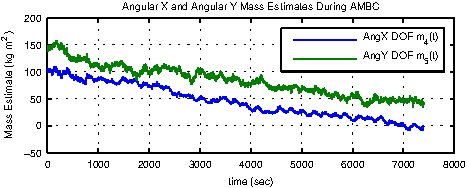
\includegraphics[width=150mm]{./chUV_AMBC/images/m4_m5_Full_Param_EstSm}
  \end{center}
  \caption{ The time evolution of Angular X \ac{DOF} and Angular Y
    \ac{DOF} mass estimates from \ac{AMBC} during 6-\ac{DOF} dynamic
    maneuvers. These mass estimates adapt to physically unrealistic
    negative values and show no signs of asymptotic behavior.}
  \label{chUV_AMBC.fig.m4_m5_Full_Param_Est}
\vspace*{-5mm}
\end{figure}
\end{center}

%\subsection{Background and Paper Contribution}

% In addition to quantifying expected performance gains, it is also
% important that experimental evaluations highlight any unfounded
% assumptions made during the controller's formulation.
% %
% As is shown in Section \ref{sec.fullAnalysisFailure}, the assumption
% that pitch and roll torque applied was close enough to torque
% commanded was not a justified assumption.
% %
% Like the \ac{JHUROV}, many vehicles currently deployed in the open ocean
% are equipped with actuators which can not guarantee the exact force
% commanded will be applied in all operating conditions.
% %
% \ac{UV} \acp{AMBC} have yet to achieve widespread use due to their perceived
% fragility in real world operating conditions.
% %
% We anticipate that this thrust reversal modeling error is one of
% several \ac{UV} \ac{AMBC} failure modes which contribute to this perception.
% %
% However, documenting one such failure mode in laboratory conditions,
% and presenting a modification to \ac{AMBC} which is robust to the
% underlying cause of failure, is an important step to developing \ac{AMBC}
% algorithms which are ready for the open ocean.



%\ac{UV} \acp{AMBC} have yet to achieve widespread use due to their perceived
%fragility in real world operating conditions.
%%
%The \ac{JHUROV}, like many vehicles currently deployed in the open ocean, 
%is equipped with actuators which can not guarantee the exact force
%commanded will be applied in all operating conditions.
%%
%In Section \ref{sec.fullAnalysisFailure} we investigate how modeling
%inaccuracies near thrust reversals can cause unstable parameter
%adaptation.
%%
%We anticipate that this thrust reversal modeling error is one of
%several \ac{UV} \ac{AMBC} failure modes which contribute to the perception of 
%\ac{AMBC} fragility.  
%%
%\hide{We feel documenting this failure mode in laboratory conditions,
%and presenting a modification to \ac{AMBC} which is robust to the
%underlying cause of failure, is an important step to developing \ac{AMBC}
%algorithms which are ready for the open ocean.}


\subsection{Unmodeled Thruster Dynamics within \\
                the \acs{UV} Control Process}

The \ac{JHUROV} control system uses the common assumption of {\it
steady-state} thruster operation when calculating the actuator
commands (see Appendix \ref{appenJHUHTF.sec.hydrolab}).
%
In {\it steady-state} operation at zero advance velocity the axial
thrust of a bladed-propeller marine thruster is linearly proportional
to the applied shaft torque, and is also linearly proportional to the
signed-square of the shaft angular-velocity
\cite{pona.book}.  
%
The parameters of these steady-state thruster models
cannot be determined analytically, but are easily estimated with
simple steady-state experiments.
%
Research has shown that the {\it transient} performance of marine
thrusters can be accurately approximated by a finite-dimensional
second-order plant model of propeller-fluid interaction.
%
The plant parameters of these dynamic thruster models cannot be
determined analytically, and are difficult to estimate experimentally
because such identification requires highly instrumented measurements
of the thruster thrust, prop angular velocity, and fluid flow velocity
in unsteady operation
\cite{yoerger.oe90,healey.joe95,bachmayer&whitcomb&grosenbaugh.joe2000,kim2006accurate}.


Because unsteady thruster model parameters are difficult to obtain
experimentally, in the design of marine vehicle control systems it is
common practice to employ easily-obtained steady-state thruster models.
%
This approach works extremely well for steady-state or slowly
time-varying vehicle motion, but results in the presence of unmodeled 
thruster dynamics during highly dynamic vehicle maneuvering.
%
In 1984, Rohrs et al. famously showed that stable adaptive controllers
for linear time-invariant plants can be destabilized by the presence
of unmodeled plant dynamics \cite{rohrs.1984}. % ,middleton1988design} 
%
To the best of our knowledge, this is the first observation of
unmodeled thruster dynamics resulting in the destabilization of
\ac{AMBC}. %model-based adaptive tracking control of an \ac{UV}.

\subsection{Comparative Experimental Evaluation of \ac{AMBC} \\
                 During Pitch-Only Motion in the Presence \\
                 of Unmodeled Thruster Dynamics}
\label{chUV_AMBC.sec.singleDOFAnalysisFailure}


This Section reports two experiments using \ac{AMBC} to control the
\ac{JHUROV}. In the first experiment parameter adaptation is unstable;
in the second experiment parameter adaptation is stable. In both
experiments the vehicle follows a pitch-only reference trajectory; the
mass, drag, and gravitational terms were initialized to parameters
previously identified to model vehicle performance (tabulated in
Tables \ref{chUV_AMBC.tb.quasistatic} and
\ref{chUV_AMBC.tb.dynParam}); and the gains used were $k_p=300$,
$k_d=100$ $\gamma_{m_i}=1000$, $\gamma_{d_i}=5000$,
$\gamma_{g}=\gamma_{b_1}=\gamma_{b_2}=0.5$ and $\gamma_{b_3}=10.0$.
In the first experiment, the pitch-only reference trajectory
oscillates about zero pitch.  In the second experiment, pitch-only
reference trajectory oscillates about a mean pitch of $5^\circ$ with
an amplitude of $3^\circ$.  The first experiment requires thrust
reversals to follow the specified reference trajectory, and the second
experiment does not require thrust reversals.

Figure \ref{chUV_AMBC.fig.stictionErrorWithThRev} plots the pitch,
angular velocity, thrust commands, and mass estimate derivative for
the experiment with thrust reversals.  In the thrust subplots the four
lines are plotted, the commanded and estimated thrusts are shown for
the two thrusters actuating vehicle pitch.  Note that the thrust is
estimated using a thruster's measured angular velocity as detailed in
Appendix \ref{appenJHUHTF.sec.hydrolab}.  Note that for both thrusters
as the commanded thrust crosses zero, the measured output remains zero
until the commanded thrust reaches 5 Newtons.  The buoyancy torque's
influence causes the pitch and y angular velocity to significantly
deviate from their respective reference trajectories.  From the
perspective of the \ac{AMBC} algorithm, these deviations from the
position and velocity reference trajectories are indistinguishable
from the deviations which would occur if the estimated pitch inertia
were too large, thus the parameter estimate update for this term,
$\dot{\hat{m}}_5$, has a large negative spike after each thrust
reversal. Over a multi-hour experiment this systematic error causes
pitch and roll mass estimates to adapt to physically unrealistic
negative values.

Figure \ref{chUV_AMBC.fig.stictionErrorWithoutThRev} plots the pitch,
angular velocity, thrust commands, and mass estimate derivative for
the experiment without thrust reversals.  Without thrust reversals,
the chain of events leading to a large negative spike in the pitch
mass update law are not present. The balanced parameter adaptation
seen in this third experiment leads to pitch mass convergence to a
physically realistic value.

%The conditions for this type of ___ also exist in the roll DOF, but not
%in the other DOF of x, y, z, Heading

\begin{center}
\begin{figure*}[htbp]
  \begin{center}
    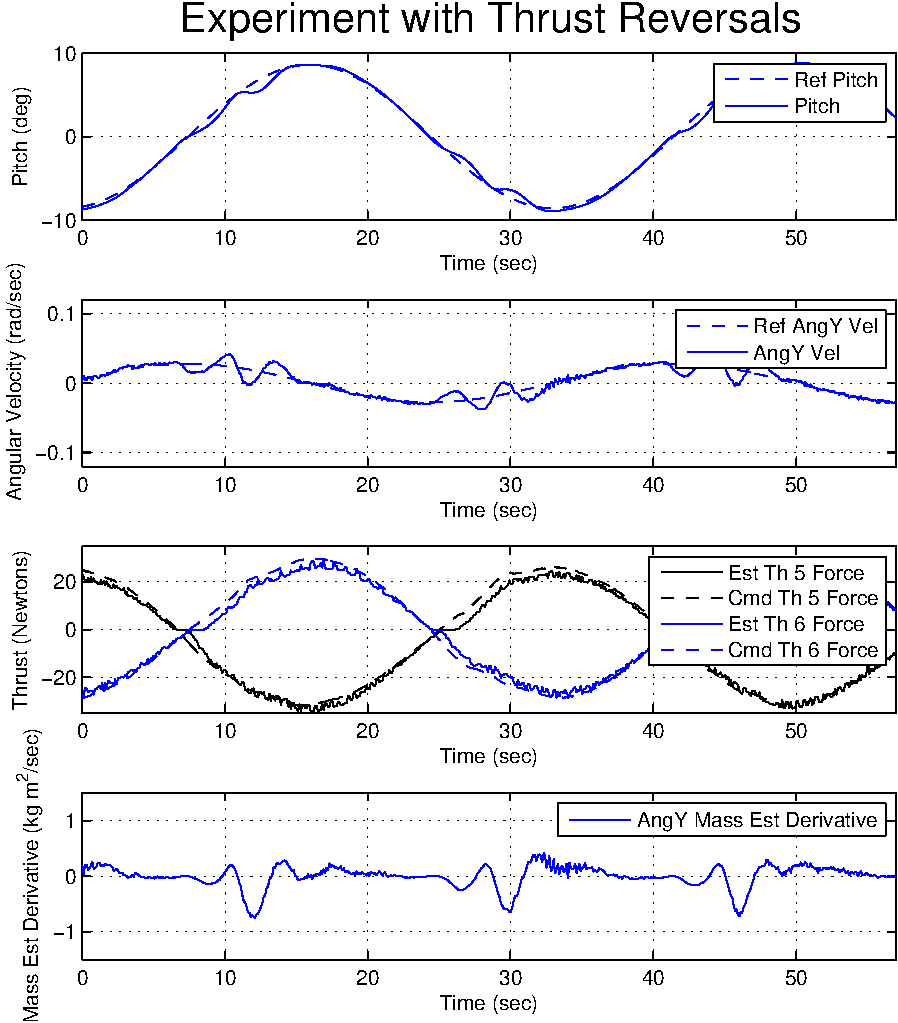
\includegraphics[width=150mm]{./chUV_AMBC/images/stictionErrorWithThrustReversals}
  \end{center}
  \caption{ 
%Data from two experiments where   For both
%    experiments an uncoupled model was assumed, initial parameter
%    estimates taken from the final values in Tables
%    \ref{chUV_AMBC.tb.quasistatic} and \ref{chUV_AMBC.tb.dynParam},
    Fifty five seconds of data from a experiment where \ac{AMBC} was used to
    follow a single \ac{DOF} reference trajectory in pitch.  Following
    the reference trajectory required thrust reversals. Thruster force
    was estimated using measured propeller angular velocity.  In the
    commanded/estimated thruster subplot, a short period of thruster
    stiction is seen at each thrust reversal.  The effects of thruster
    stiction are seen in both the pitch and angular velocity plots as
    deviations from each state's respective reference trajectory. In
    the pitch mass estimate derivative, the parameter update law is
    seen to have a large negative spike after each thrust reversal.}
  \label{chUV_AMBC.fig.stictionErrorWithThRev}
\end{figure*}
\end{center}

\begin{center}
\begin{figure*}[htbp]
  \begin{center}
    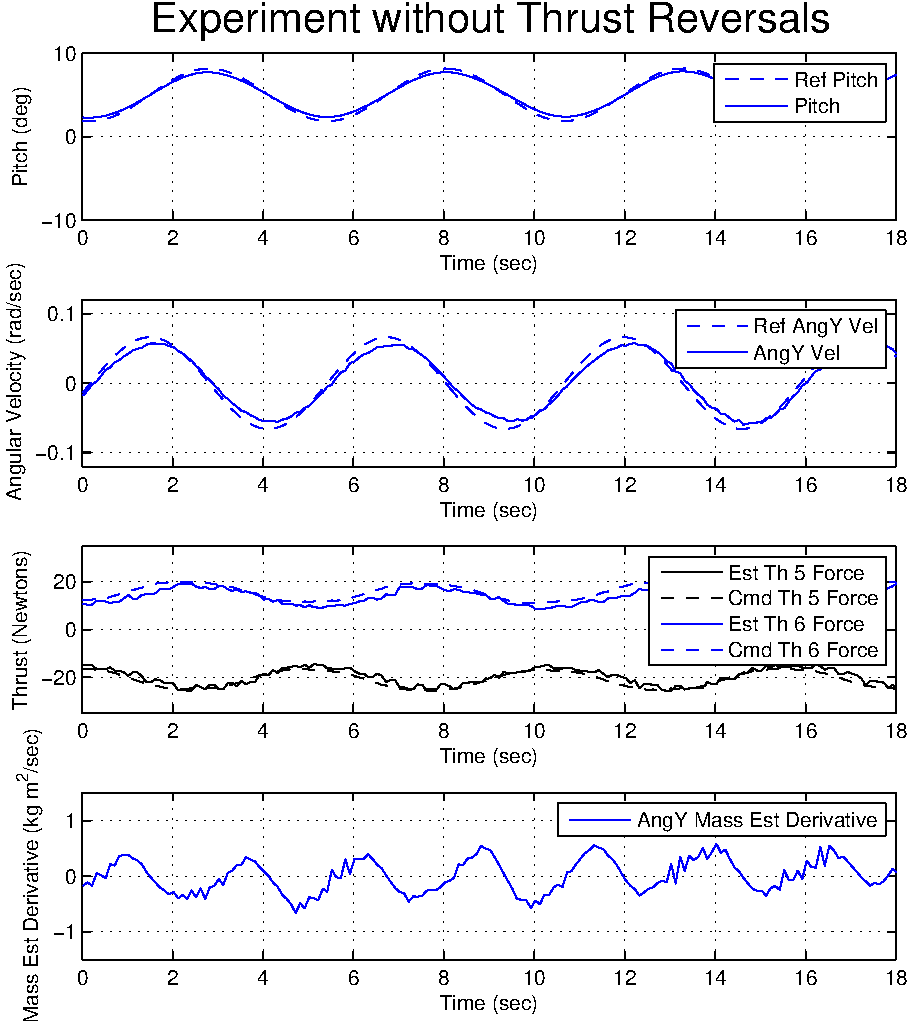
\includegraphics[width=150mm]{./chUV_AMBC/images/stictionErrorWoThrustReversals}
  \end{center}
  \caption{Eighteen seconds of data from a experiment where \ac{AMBC} was
    used to follow a single \ac{DOF} reference trajectory in pitch.
    Following the reference trajectory did not require thrust
    reversals. Thruster force was estimated using measured propeller
    angular velocity.  In the commanded/estimated thruster subplot
    thruster stiction is not observed.  The chain of events leading to a
    large negative spike in the pitch mass update law are not present
    in this experiment.}
  \label{chUV_AMBC.fig.stictionErrorWithoutThRev}
\end{figure*}
\end{center}

%experimental.tex
%\section{Experimental Evaluation}\label{sec.experimental}



\subsection{Experimental Evaluation of Two-Step Method}
\label{chUV_AMBC.sec.twoStepExp}

In this Section we report an experimental evaluation of the two-step
algorithm reported in Section \ref{chUV_AMBC.sec.twoStepMethod}.

The first step is identifying the gravitational and buoyancy
parameters for the \ac{UV} using the adaptive tracking controller for
plant model (\ref{chUV_AMBC.eq.plantQS}).  The reference trajectory
was constant in translational position and heading, with slow changes
in pitch and roll to provide quasi-static motion.  For this experiment
we used a sinusoidal pitch reference trajectory with a magnitude of
$0.2$ rad and frequency of $34$ Hz and a sinusoidal roll reference
trajectory with a magnitude of $0.15$ rad and frequency of $42$
Hz. The gains used were $k_p=300$, $k_d=100$,
$\gamma_{g}=\gamma_{b_1}=\gamma_{b_2}=0.5$, and $\gamma_{b_3}=10.0$.
Over a 90 minute experiment the gravitational and buoyancy parameters
were stable and converged to the physically realistic values shown in
Table \ref{chUV_AMBC.tb.quasistatic}.

\begin{table}[htbp]
\ssp
\caption{Gravitational Parameters Identified During Quasi-Static Motion}
\begin{center}
\begin{tabular}{c|cccc}
 & $g$ & $b_1$ & $b_2$ & $b_3$ \\
 & {\it N} & {\it N m} & {\it N m} & {\it N m} \\ \hline
Final & 3.59 & 1.696 & 3.09 & 300 \\
\end{tabular}
\end{center}
\label{chUV_AMBC.tb.quasistatic}
\vspace*{-5mm}
\end{table}


The second step uses the identified parameters from Table
\ref{chUV_AMBC.tb.quasistatic} in a \ac{AMBC} which estimates the
mass and drag parameters, as described in Section
\ref{chUV_AMBC.sec.twoStepMethod}.
%
In the second step of the two-step \ac{AMBC} algorithm the reference
trajectory specified was RefTraj1 from Table
\ref{chUV_AMBC.tb.expStat}; the mass and drag parameters were
initialized to zero; and the gains used were $k_p=300$, $k_d=1000$,
$\gamma_{m_i}=1000$, and $\gamma_{d_i}=5000$.  Over a four and a half
hour experiment all 12 mass and drag parameters were observed to be
stable and converge to physically realistic values.  Table
\ref{chUV_AMBC.tb.dynParam} records the initial and final states for
each dynamic parameter estimate.

\begin{table}[htbp]
\ssp
\caption{Parameters Identified with two-step \ac{AMBC} during 
  Dynamic Motion Trajectory-Tracking}
\begin{center}
\begin{tabular}{c|cccc}
 & $m_i(t_o)$ & $m_i(t_f)$ & $d_i(t_o)$ & $d_i(t_f)$ \\ \hline
Trans X \ac{DOF} & 0.0 {\it kg}& 628 {\it kg}& 0.0 {\it $\frac{\text{N}~\text{s}^2}{\text{m}^2}$}& -1259 {\it $\frac{\text{N}~\text{s}^2}{\text{m}^2}$}\\
Trans Y \ac{DOF} & 0.0 {\it kg}& 791 {\it kg}& 0.0 {\it $\frac{\text{N}~\text{s}^2}{\text{m}^2}$}& -1429 {\it $\frac{\text{N}~\text{s}^2}{\text{m}^2}$}\\
Trans Z \ac{DOF} & 0.0 {\it kg}&1043 {\it kg}& 0.0 {\it $\frac{\text{N}~\text{s}^2}{\text{m}^2}$}& -3083 {\it $\frac{\text{N}~\text{s}^2}{\text{m}^2}$}\\
Angular X \ac{DOF} & 0.0 {\it kg $\text{m}^2$}& 95.7 {\it kg $\text{m}^2$}& 0.0 {\it N $\text{s}^2$}& -727.1 {\it N $\text{s}^2$}\\
Angular Y \ac{DOF} & 0.0 {\it kg $\text{m}^2$}& 145.3 {\it kg $\text{m}^2$}& 0.0 {\it N $\text{s}^2$}& -783.4 {\it N $\text{s}^2$}\\
Angular Z \ac{DOF} & 0.0 {\it kg $\text{m}^2$}& 110.2 {\it kg $\text{m}^2$}& 0.0 {\it N $\text{s}^2$}& -465.6 {\it N $\text{s}^2$}\\
\end{tabular}
\end{center}
\label{chUV_AMBC.tb.dynParam}
\vspace*{-5mm}
\end{table}

\subsubsection{Two-Step \ac{AMBC} Trajectory Tracking Performance}

Figure \ref{chUV_AMBC.fig.MNE_All} compares the performance of the
second step of the two-step \ac{AMBC} to a \ac{PDC} with comparable
gains.  These two plots contain the exponential position and velocity
\ac{MNE} for the \ac{PDC} and two-step \ac{AMBC} experimental run.
Both controllers were following the reference trajectory RefTraj1 from
Table \ref{chUV_AMBC.tb.expStat} as well as using $k_p=300$ and
$k_d=100$.
%
The \ac{PDC} \acp{MNE} values were calculated using 10 minutes of
data.  
%
The two-step \ac{AMBC} \acp{MNE} values were calculated
for consecutive 15 minutes windows.
%
Note that after parameter convergence the two-step \ac{AMBC} provides
$30\%$ better position tracking and $8\%$ worse velocity tracking than
\ac{PDC} with similar gains.
%
% Thus two-step \ac{AMBC} Since position trajectory tracking is typically
% the goal of current \ac{UV} controllers, this controller provides
% significant advantages over standard \ac{PDC} control method for 6-\ac{DOF}
% motion.

Table \ref{chUV_AMBC.tb.trajTrackMAE} reports the trajectory tracking
\ac{MAE} values of individual \ac{DOF} for both the \ac{PDC} and
two-step \ac{AMBC} experiments.
%
The \ac{PDC} \acp{MAE} values were calculated using 10 minutes of
data.  
%
The two-step \ac{AMBC} \acp{MAE} values were calculated
for consecutive 15 minutes windows.
%
For each of the position \ac{DOF}, two-step \ac{AMBC} \ac{MAE} values
were smaller than \ac{PDC} values.
%
With the exception of heading, two-step \ac{AMBC} position trajectory
tracking improved in each \ac{DOF} as the parameter adaptation process
progressed.
%
Of the velocity \ac{DOF}, two-step \ac{AMBC} only outperformed
\ac{PDC} in the x and y angular velocity \ac{DOF}.
%
With the exception of y angular velocity, two-step \ac{AMBC} velocity
trajectory-tracking performance degraded slightly as the parameter
adaptation process occurred.
%
For the \ac{DOF} in which trajectory-tracking is not improving, this
could be an effect of unmodeled thruster dynamics or other dynamics
which are not included in the uncoupled lumped-parameter model of
\ac{UV} dynamics used in our \ac{AMBC} algorithm.
%
However, taken as a whole, this experimental evaluation indicates that
\ac{AMBC} can provide increased trajectory-tracking performance in the
presence of unmodeled thruster dynamics.




\begin{center}
\begin{figure}[htbp]
  \begin{center}
    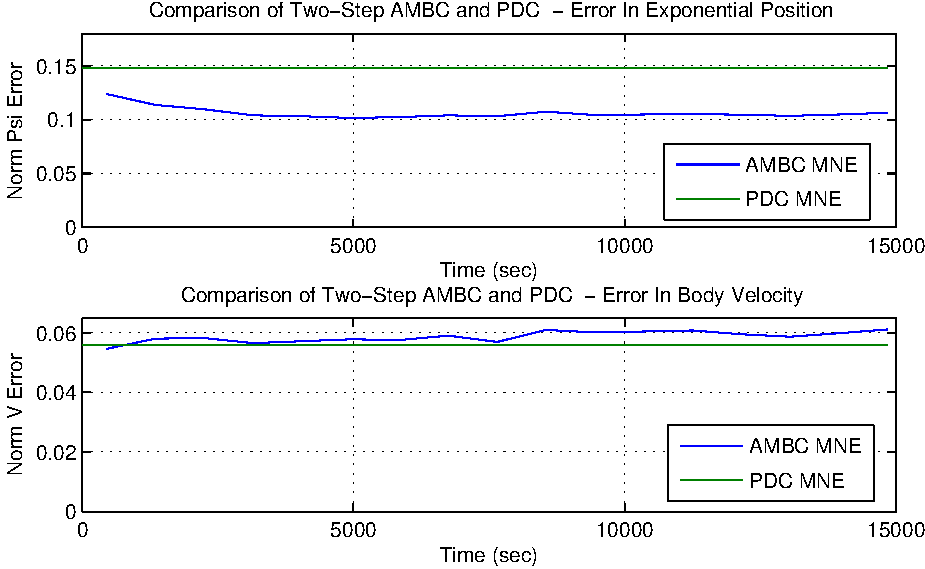
\includegraphics[width=150mm]{./chUV_AMBC/images/MNE_All}
  \end{center}
  \caption{ Exponential position and velocity \ac{MNE} values for the
    experimental evaluations of two controllers, \ac{PDC} and two-step
    \ac{AMBC}.  Both controllers were following the same reference
    trajectory (RefTraj1 from Table \ref{chUV_AMBC.tb.expStat}) as
    well as using the gains $k_p=300$ and $k_d=100$.  The \ac{PDC}
    \ac{MNE} values were calculated using 10 minutes of data, this
    single value is plotted in green across the entire figure.  The
    two-step \ac{AMBC} \ac{MNE} values were calculated for consecutive
    15 minute windows and plotted in blue. }
  \label{chUV_AMBC.fig.MNE_All}
\vspace*{-5mm}
\end{figure}
\end{center}

% \begin{sidewaystable*}
% \ssp
% \fontsize{8pt}{8pt}\selectfont
% \caption{Mean Absolute Error values over different pieces on time.}
% \begin{center}
% \begin{tabular}{c|ccccccccccccc} 
%     Parameter & Time  &&&&&&&&&&&& \\              
%           Set & Block & PosX & PosY & PosZ & Hea & Pit & Rol & BodVelX & BodVelY & BodVelZ & AngVelX & AngVelY & AngVelZ \\ \hline 
% \\
% \ac{PDC} Exp  &      ALL   & 0.076m & 0.061m & 0.058m & 0.028rad & 0.047rad & 0.04rad & 0.0172m/s & 0.021m/s & 0.0156m/s & 0.021rad/s & 0.028rad/s & 0.0078rad/s \\ \hline
% \\
% \ac{AMBC} Exp & 0-14 min & 0.059m & 0.051m & 0.064m & 0.021rad & 0.023rad & 0.0181rad & 0.022m/s & 0.023m/s & 0.0194m/s & 0.0136rad/s & 0.017rad/s & 0.0134rad/s \\
% \\
% \ac{AMBC} Exp & 0-14 min & 0.051m & 0.045m & 0.063m & 0.022rad & 0.0196rad & 0.0184rad & 0.024m/s & 0.023m/s & 0.02m/s & 0.0137rad/s & 0.0157rad/s & 0.0162rad/s \\
% \\
% \ac{AMBC} Exp & 15-29 min & 0.047m & 0.046m & 0.057m & 0.021rad & 0.0196rad & 0.0171rad & 0.023m/s & 0.025m/s & 0.02m/s & 0.013rad/s & 0.0169rad/s & 0.0153rad/s \\
% \\
% \ac{AMBC} Exp & 30-44 min & 0.046m & 0.045m & 0.054m & 0.0192rad & 0.018rad & 0.0165rad & 0.023m/s & 0.025m/s & 0.0196m/s & 0.0136rad/s & 0.0157rad/s & 0.0149rad/s \\
% \\
% \ac{AMBC} Exp & 45-59 min & 0.046m & 0.043m & 0.052m & 0.021rad & 0.0174rad & 0.0162rad & 0.024m/s & 0.025m/s & 0.019m/s & 0.0136rad/s & 0.0162rad/s & 0.0161rad/s \\
% \\
% \ac{AMBC} Exp & 60-74 min & 0.047m & 0.047m & 0.046m & 0.0198rad & 0.0174rad & 0.0156rad & 0.023m/s & 0.027m/s & 0.0179m/s & 0.0138rad/s & 0.0168rad/s & 0.0152rad/s \\
% \\
% \ac{AMBC} Exp & 75-89 min & 0.047m & 0.045m & 0.05m & 0.021rad & 0.0168rad & 0.0155rad & 0.024m/s & 0.024m/s & 0.0192m/s & 0.0143rad/s & 0.0164rad/s & 0.0155rad/s \\
% \\
% \ac{AMBC} Exp & 90-104 min & 0.046m & 0.046m & 0.052m & 0.022rad & 0.0174rad & 0.0155rad & 0.024m/s & 0.026m/s & 0.0198m/s & 0.014rad/s & 0.0165rad/s & 0.0162rad/s \\
% \\
% \ac{AMBC} Exp & 105-119 min & 0.048m & 0.044m & 0.05m & 0.022rad & 0.0162rad & 0.0153rad & 0.021m/s & 0.025m/s & 0.021m/s & 0.0133rad/s & 0.0159rad/s & 0.0151rad/s \\
% \\
% \ac{AMBC} Exp & 120-134 min & 0.049m & 0.048m & 0.054m & 0.021rad & 0.0182rad & 0.015rad & 0.023m/s & 0.027m/s & 0.023m/s & 0.0145rad/s & 0.0169rad/s & 0.016rad/s \\
% \\
% \ac{AMBC} Exp & 135-149 min & 0.049m & 0.045m & 0.05m & 0.022rad & 0.0177rad & 0.0145rad & 0.025m/s & 0.026m/s & 0.021m/s & 0.0145rad/s & 0.0172rad/s & 0.0165rad/s \\
% \\
% \ac{AMBC} Exp & 150-164 min & 0.05m & 0.046m & 0.049m & 0.021rad & 0.0166rad & 0.0155rad & 0.024m/s & 0.026m/s & 0.021m/s & 0.0143rad/s & 0.0161rad/s & 0.0167rad/s \\
% \\
% \ac{AMBC} Exp & 165-179 min & 0.049m & 0.046m & 0.052m & 0.021rad & 0.0168rad & 0.0151rad & 0.024m/s & 0.026m/s & 0.022m/s & 0.0145rad/s & 0.0167rad/s & 0.0153rad/s \\
% \\
% \ac{AMBC} Exp & 180-194 min & 0.048m & 0.047m & 0.05m & 0.021rad & 0.017rad & 0.0149rad & 0.024m/s & 0.024m/s & 0.021m/s & 0.0141rad/s & 0.0165rad/s & 0.016rad/s \\
% \\
% \ac{AMBC} Exp & 195-209 min & 0.05m & 0.045m & 0.049m & 0.022rad & 0.0169rad & 0.0149rad & 0.023m/s & 0.026m/s & 0.02m/s & 0.0139rad/s & 0.0163rad/s & 0.0161rad/s \\
% \\
% \ac{AMBC} Exp & 210-224 min & 0.05m & 0.046m & 0.049m & 0.021rad & 0.0174rad & 0.0147rad & 0.024m/s & 0.027m/s & 0.021m/s & 0.0142rad/s & 0.0166rad/s & 0.0148rad/s \\
% \\
% \ac{AMBC} Exp & 225-239 min & 0.047m & 0.046m & 0.054m & 0.022rad & 0.0172rad & 0.0147rad & 0.025m/s & 0.026m/s & 0.023m/s & 0.0145rad/s & 0.0164rad/s & 0.0169rad/s \\
% \end{tabular}
% \end{center}
% \label{chUV_AMBC.tb.MAE}
% \end{sidewaystable*}


\begin{sidewaystable*}
\ssp
\fontsize{10pt}{10pt}\selectfont
\caption{\acf{MAE} values for both the \ac{PDC} and two-step \ac{AMBC}
  experiments.  The \ac{MAE} for each \ac{DOF} is shown. 10 minutes of
  experimental data were used to calculate the \ac{PDC} \acp{MAE}.
  \ac{AMBC} \acp{MAE} were calculated for consecutive 15 minute
  windows spread over the 3 hour experiment.}
\begin{center}
\begin{tabular}{c|ccccccccccccc} 
    Parameter & Time  &&&&&&&&&&&& \\              
          Set & Block & PosX & PosY & PosZ & Hea & Pit & Rol & BodVelX & BodVelY & BodVelZ & AngVelX & AngVelY & AngVelZ \\  
      {\it -} & {\it min} & {\it m}   &  {\it m}  &  {\it m}  &{\it rad} &{\it rad} &{\it rad} &{\it m/sec} &{\it m/sec} &{\it m/sec} &{\it rad/sec} &{\it rad/sec} &{\it rad/sec} \\ \hline 
\\
\ac{PDC} Exp  &    -   & 0.076  & 0.061  & 0.058  & 0.028  & 0.047  & 0.04  & 0.0172  & 0.021  & 0.0156  & 0.021  & 0.028  & 0.0078  \\ \hline
\\
\ac{AMBC} Exp & 0-14   & 0.059  & 0.051  & 0.064  & 0.021  & 0.023  & 0.0181  & 0.022  & 0.023  & 0.0194  & 0.0136  & 0.017  & 0.0134  \\
\\
\ac{AMBC} Exp & 15-29   & 0.051  & 0.045  & 0.063  & 0.022  & 0.0196  & 0.0184  & 0.024  & 0.023  & 0.02  & 0.0137  & 0.0157  & 0.0162  \\
\\
\ac{AMBC} Exp & 30-44   & 0.047  & 0.046  & 0.057  & 0.021  & 0.0196  & 0.0171  & 0.023  & 0.025  & 0.02  & 0.013  & 0.0169  & 0.0153  \\
\\
\ac{AMBC} Exp & 45-59   & 0.046  & 0.045  & 0.054  & 0.0192  & 0.018  & 0.0165  & 0.023  & 0.025  & 0.0196  & 0.0136  & 0.0157  & 0.0149  \\
\\
\ac{AMBC} Exp & 60-74   & 0.046  & 0.043  & 0.052  & 0.021  & 0.0174  & 0.0162  & 0.024  & 0.025  & 0.019  & 0.0136  & 0.0162  & 0.0161  \\
\\
\ac{AMBC} Exp & 75-89   & 0.047  & 0.047  & 0.046  & 0.0198  & 0.0174  & 0.0156  & 0.023  & 0.027  & 0.0179  & 0.0138  & 0.0168  & 0.0152  \\
\\
\ac{AMBC} Exp & 90-104   & 0.047  & 0.045  & 0.05  & 0.021  & 0.0168  & 0.0155  & 0.024  & 0.024  & 0.0192  & 0.0143  & 0.0164  & 0.0155  \\
\\
\ac{AMBC} Exp & 105-119   & 0.046  & 0.046  & 0.052  & 0.022  & 0.0174  & 0.0155  & 0.024  & 0.026  & 0.0198  & 0.014  & 0.0165  & 0.0162  \\
\\
\ac{AMBC} Exp & 120-134  & 0.048  & 0.044  & 0.05  & 0.022  & 0.0162  & 0.0153  & 0.021  & 0.025  & 0.021  & 0.0133  & 0.0159  & 0.0151  \\
\\
\ac{AMBC} Exp & 135-149   & 0.049  & 0.048  & 0.054  & 0.021  & 0.0182  & 0.015  & 0.023  & 0.027  & 0.023  & 0.0145  & 0.0169  & 0.016  \\
\\
\ac{AMBC} Exp & 150-164   & 0.049  & 0.045  & 0.05  & 0.022  & 0.0177  & 0.0145  & 0.025  & 0.026  & 0.021  & 0.0145  & 0.0172  & 0.0165  \\
\\
\ac{AMBC} Exp & 165-179   & 0.05  & 0.046  & 0.049  & 0.021  & 0.0166  & 0.0155  & 0.024  & 0.026  & 0.021  & 0.0143  & 0.0161  & 0.0167  \\
\\
\ac{AMBC} Exp & 180-194   & 0.049  & 0.046  & 0.052  & 0.021  & 0.0168  & 0.0151  & 0.024  & 0.026  & 0.022  & 0.0145  & 0.0167  & 0.0153  \\
\\
\ac{AMBC} Exp & 195-209   & 0.048  & 0.047  & 0.05  & 0.021  & 0.017  & 0.0149  & 0.024  & 0.024  & 0.021  & 0.0141  & 0.0165  & 0.016  \\
\\
\ac{AMBC} Exp & 210-224   & 0.05  & 0.045  & 0.049  & 0.022  & 0.0169  & 0.0149  & 0.023  & 0.026  & 0.02  & 0.0139  & 0.0163  & 0.0161  \\
\\
\ac{AMBC} Exp & 225-239   & 0.05  & 0.046  & 0.049  & 0.021  & 0.0174  & 0.0147  & 0.024  & 0.027  & 0.021  & 0.0142  & 0.0166  & 0.0148  \\
\\
\ac{AMBC} Exp & 240-255   & 0.047  & 0.046  & 0.054  & 0.022  & 0.0172  & 0.0147  & 0.025  & 0.026  & 0.023  & 0.0145  & 0.0164  & 0.0169  \\
\end{tabular}
\end{center}
\label{chUV_AMBC.tb.trajTrackMAE}
\end{sidewaystable*}


\subsubsection{Two-Step \ac{AMBC} Parameter Cross-Validation}

In addition to providing trajectory-tracking, \ac{AMBC} has also been
proposed to identify \ac{UV} models.
%
Two questions arise: 
%
\begin{itemize}
\item ``How good is the identified model at reproducing vehicle performance?''
%``When considering the time series of parameter
%estimations, will the capacity of the models which used these
%parameter estimations get better at matching vehicle performance as
%time increases?''
%
\item``Considering the time series of parameter estimates, do the
  resulting plant models get better at matching \ac{JHUROV}
  performance as the parameter adaptation process progresses?''
\end{itemize}
%

To address these questions we preformed a cross-validation experiment
(Appendix \ref{appenJHUHTF.sec.paramEvalMethod}) by driving the
\ac{JHUROV} to follow RefTraj2 from Table \ref{chUV_AMBC.tb.expStat}.
%the \ac{UV} states and thrust inputs were recorded for 10 minutes.
%
\Cref{chUV_AMBC.fig.posOLO,chUV_AMBC.fig.angVelOLO,chUV_AMBC.fig.bodVelOLO}
show the ability of the identified model to match vehicle performance
in forward simulation increases during parameter adaptation.
%
Each Figure shows experimentally measured states verses the states
from numerical simulations; each numerical simulation uses a model
identified by the two-step \ac{AMBC} after a set amount of time.
%
Each \ac{JHUROV} simulation used the thrust inputs recorded and
initial \ac{JHUROV} states to create a forward
simulation. % of vehicle performance.
%
All eight open-loop-stable states are plotted.
%
In both the plots and listed \ac{MAE} values, the capacity of the
identified parameters to model vehicle performance in every \ac{DOF}
increases as time progresses.
%
The fact that the parameter estimates are progressively improving
suggests that the parameter adaptation process is working despite the
presence of unmodeled thruster dynamics.



As was seen with \ac{AID} and \ac{LS} in Sections
\ref{chUV_AID.sec.UVSO3exp} and \ref{chUV_AID.sec.UVSE3exp}, the
models identified using two-step \ac{AMBC} were not able to reproduce
the highest frequency fluctuation's observed experimentally (such as
those seen in the x angular velocity subplots of Figure
\ref{chUV_AMBC.fig.angVelOLO}).
%
However, the states shown from simulating a model using the ``5000
sec'' parameter set (the final parameter set included in this
analysis) indicate that \ac{AMBC} can produce parameter estimates
which result in accurate plant models.




\begin{center}
\begin{figure}[htbp]
  \begin{center}
    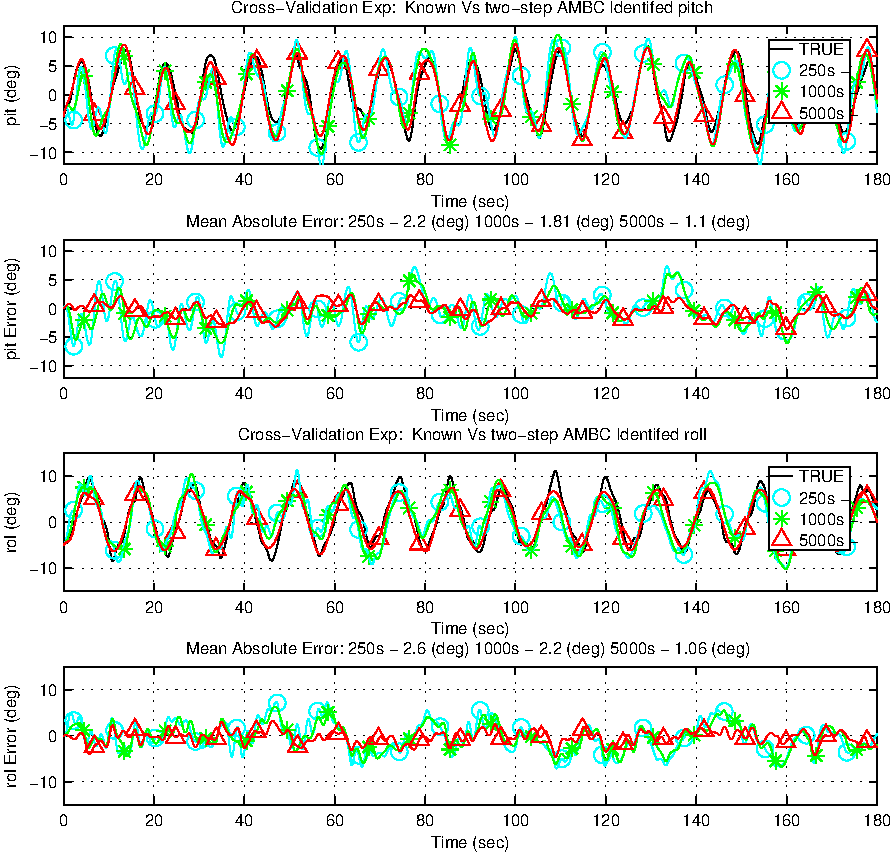
\includegraphics[width=150mm]{./chUV_AMBC/images/OLO_angPos}
  \end{center}
  \caption{ Representative data of experimental and simulated
    \ac{JHUROV} states during 6-\ac{DOF} dynamic operation.  In the
    roll and pitch plots the measured state is plotted together with
    the position estimates from three \ac{JHUROV} simulations. The
    three parameter sets were taken from the time history of parameter
    adaptation recorded during the two-step \ac{AMBC} experiment.  The
    '250s' forward simulation (plotted in blue and marked with
    circles) models \ac{JHUROV} performance using parameters
    identified after 250 seconds of parameter adaptation.  Similarly
    the '1000s' forward simulation (plotted in green and marked with
    stars) and '5000s' forward simulation (plotted in red and marked
    with triangles) use parameters identified after 1000 and 5000
    seconds of parameter adaptation respectively.  For each \ac{DOF},
    the error between the measured positions and their estimates is
    shown.  }
  \label{chUV_AMBC.fig.posOLO}
\end{figure}
\end{center}

\begin{center}
\begin{figure}[htbp]
  \begin{center}
    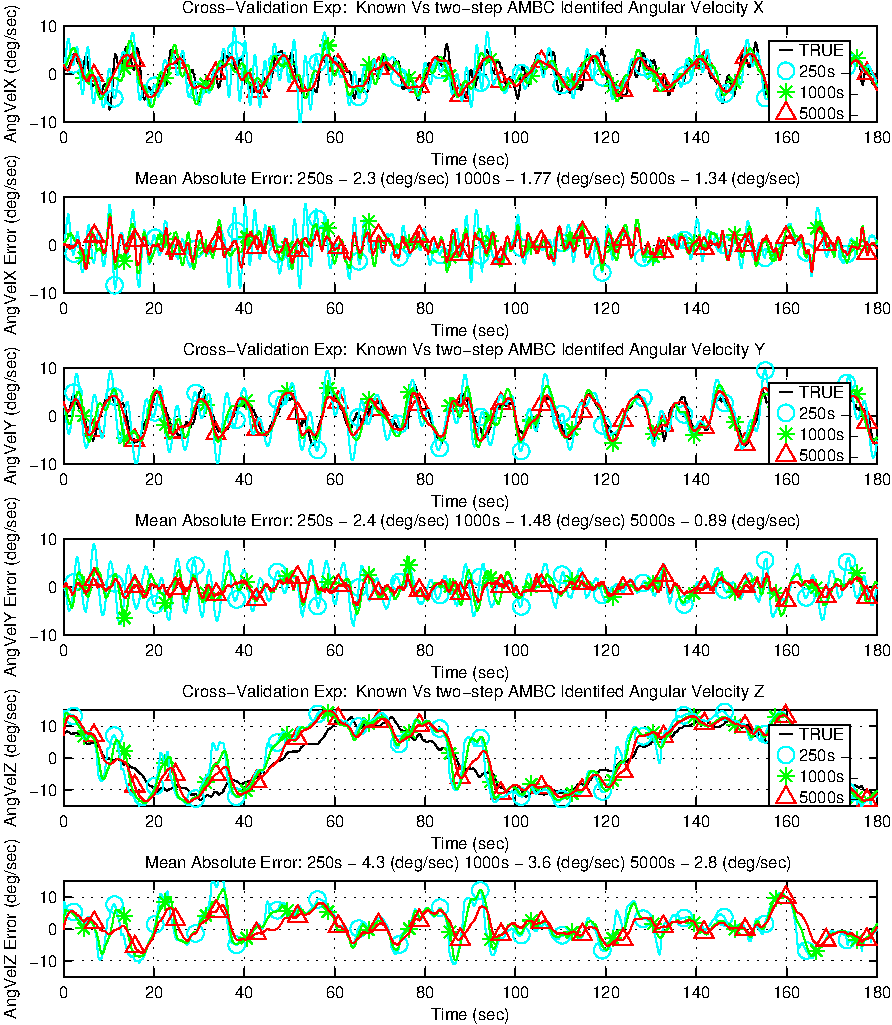
\includegraphics[width=150mm]{./chUV_AMBC/images/OLO_angVel}
  \end{center}
  \caption{ Representative data of experimental and simulated
    \ac{JHUROV} states during 6-\ac{DOF} dynamic operation.  In the
    three angular velocity plots, the measured state is plotted
    together with the velocity estimates from three \ac{JHUROV}
    simulations. The three parameter sets were taken from the time
    history of parameter adaptation recorded during the two-step
    \ac{AMBC} experiment.  See Figure \ref{chUV_AMBC.fig.posOLO}
    caption for further information on each parameter set.  For each
    \ac{DOF}, the error between the measured positions and their
    estimates is shown.  }
  \label{chUV_AMBC.fig.angVelOLO}
\end{figure}
\end{center}

\begin{center}
\begin{figure}[htbp]
  \begin{center}
    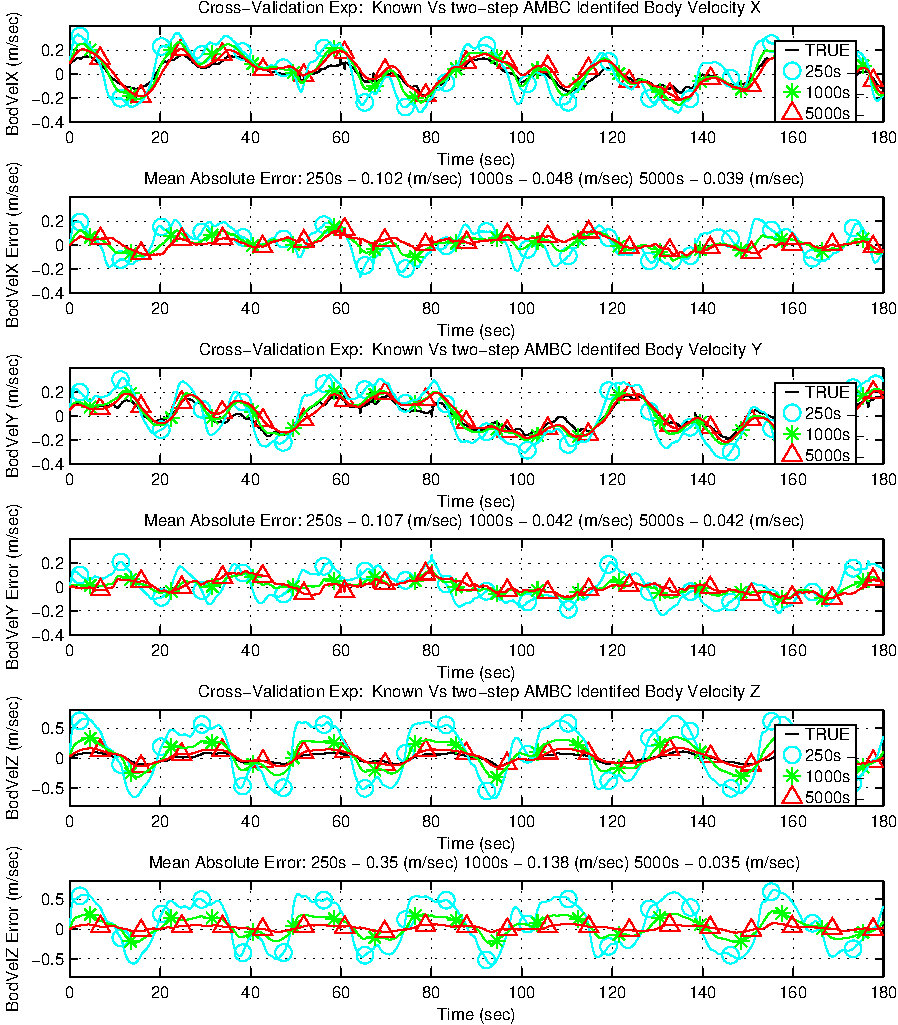
\includegraphics[width=150mm]{./chUV_AMBC/images/OLO_bodyVel}
  \end{center}
  \caption{ Representative data of experimental and simulated
    \ac{JHUROV} states during 6-\ac{DOF} dynamic operation.  In the
    three body velocity plots, the measured state is plotted together
    with the velocity estimates from three \ac{JHUROV}
    simulations. The three parameter sets were taken from the time
    history of parameter adaptation recorded during the two-step
    \ac{AMBC} experiment.  See Figure \ref{chUV_AMBC.fig.posOLO}
    caption for further information on each parameter set.  For each
    \ac{DOF}, the error between the measured positions and their
    estimates is shown.  }
  \label{chUV_AMBC.fig.bodVelOLO}
\end{figure}
\end{center}
 


\subsection{The Effects of Unmodeled Thruster Dynamics on \ac{AMBC}}

The experiment reported in Section
\ref{chUV_AMBC.sec.fullAnalysisFailure} shows, curiously, a clear
differentiation in parameter adaptation performance; unstable
parameter adaption occurred only in the parameter estimates associated
with pitch and roll dynamics.
%
To further explore this effect, in Section
\ref{chUV_AMBC.sec.singleDOFAnalysisFailure} we investigated parameter
adaptation during pitch-only reference trajectory excitation.
%
These data show thrust reversals cause parameter instability.
%
Further, the thruster angular velocity data indicate a difference
between the actual and commanded torques applied to the vehicle. 
%
Based on our knowledge of the \ac{JHUROV} control system and thruster
design, the data from these pitch-only experiments suggest that
unmodeled thruster dynamics are present during thrust reversals.
%
Without further experimental analysis we can not specify if the
specific mechanism causing unstable parameter adaptation is unmodeled
thruster mechanical dynamics, fluid dynamics, mechanical friction
during thrust reversals, or some combination of these mechanisms.
%
Regardless of the underlying source of modeling error, these
experiments suggest that unstable parameter adaptation will occur in
parameters associated with a given \ac{DOF} if the following three
conditions are met:
%
\begin{itemize}
\item mass and gravitational parameter estimates are adapting, 
\item there exists of a single attractive stability point for that \ac{DOF}, and
\item unmodeled thruster dynamics are present.
\end{itemize}


The success of two-step parameter adaptation supports this hypothesis.
%
Implementing the parameter estimation process in two steps removed
the need for simultaneous adaptation of the mass and buoyancy terms.
%
By separating parameter adaptation in this way, an ambiguity in the
adaptation process was removed.
%
Note the three factors listed imply that both the buoyancy and
mass parameter estimates will be affected in the same way by unmodeled
thruster dynamics during thrust reversals.  
%
From the perspective of the \ac{AMBC} algorithm, the deviations from
the position and velocity reference trajectories caused by unmodeled
thruster dynamics are indistinguishable from the deviations which
would occur if either of these parameter estimates (the buoyancy
torque estimate or the inertia estimate) were too large.
%
The effects of the inertia tensor and buoyancy torque parameters on
vehicle position and velocity are also coupled.
%
For instance there will be similarities between the dynamics of a
\ac{UV} with a large mass and large buoyancy torque and a \ac{UV} with
a small mass and small buoyancy torque for a proper scaling of these
properties.
%
During each period of unmodeled thruster dynamics, the simultaneous
unstable adaptation of the inertia and buoyancy estimates was
difficult for the \ac{AMBC} algorithm to overcome because the estimate
of vehicle dynamics was only slightly degraded by the physically
unrealistic changes in these parameter estimates.
%
Setting the buoyancy torque estimate to a fixed value during dynamic
maneuvers removes the possibility of simultaneous adaptation to
physically unrealistic values.






%  might still be close to values which are
% still good at approximating vehicle dynamics.
% %
% However, the difference tween
 
% adapt twoards physically unrealistic parameter values togeather, the
% difference in vehicle dynamnics

% Although these parameters play structrually
% different roles in UV dynamics their effects on the

% their effects for small angles are coupled,  that much
% of the UV modeling errors both having physically unrealstic values can


%  a different form when entering
% into the dynamics equation



%  or the if the
% estimated pitch inertia were too large both parameter update laws will
% experience a large negitive spike since the pitch or roll state
% lingering near zero

% Although   

%conclusion.tex
\section{Conclusion}  \label{chUV_AMBC.sec.conclusion}

This Chapter presents both theoretical and experimental results
concerning \ac{UV} \ac{AMBC}.
%
Section \ref{chUV_AMBC.sec.theory} reports \ac{MBC} and \ac{AMBC}
algorithms, along with a local proofs of stability.
%
Section \ref{chUV_AMBC.sec.unmodeledActDyn} reports an experimental
investigation of a previously unreported \ac{UV} \ac{AMBC} failure
mode where unmodeled thruster dynamics during thrust reversals cause
unstable parameter adaptation.
%
The Section also reports a novel two-step \ac{AMBC} algorithm which is
shown experimentally to provide stable trajectory tracking and
parameter adaptation in the presence of the unmodeled thruster
dynamics of our system.
%
Finally, it reports a comparative experimental analysis of the
two-step \ac{AMBC} algorithm with \ac{PDC}.
%
This experimental evaluation shows that two-step \ac{AMBC} provides
30\% better position tracking performance and 8\% worse velocity
tracking performance over \ac{PDC}.

\chapter{Conclusion}
\label{chConc}
\chaptermark{Conclusion}
%\ssp
\acresetall

\section{Thesis Summary}


This Thesis reports algorithms for state estimation, adaptive
parameter identification, and model-based control  principally for
\ac{UV} applications.
%
An analytical proof of stability is included for every reported algorithm.
%
Chapter \ref{chSMS_ID} reports an angular velocity observer for
rotating rigid-bodies, an \ac{AID} algorithm for rotating rigid-bodies,
and an \ac{AID} algorithm for \acp{OKC}.
%
Numerical simulations of the \ac{AID} algorithm for rotating
rigid-bodies corroborate the analytical stability analysis and
investigate parameter convergence with varying initial conditions,
adaptation gains, and input torques.
%
Chapter \ref{chSMS_ID} also reports a comparative analysis of three
nonlinear angular velocity observer for rotating rigid-bodies; in
numeric simulations the novel angular velocity observer (Theorem
\ref{chSMS_ID.theo.AVO_Theorem}) is shown to provide performance
similar to that of the two previously reported observers.


Chapter \ref{chUV_AID} reports two \ac{AID} algorithms for the dynamic
estimation of \ac{UV} plant parameters.
%
Chapter \ref{chUV_AID} also reports two comparative experimental
evaluations of \acl{AID} and \acl{LS}.
%
Both the \acp{AIDPM} and the \acp{LSPM} are shown to match closely the
experimentally observed \ac{UV} input-output behavior.
%
Adaptive identification algorithms do not require simultaneous
reference trajectory-tracking control, nor do they require
instrumentation of linear acceleration or angular acceleration.
%
Together, these facts make adaptive identification applicable to a
wider class of \acp{UV} than previously reported methods.
%
Chapter \ref{chUV_AMBC} reports an \ac{UV} \ac{MBC} algorithm and
\ac{UV} \ac{AMBC} algorithm.  
%
Chapter \ref{chUV_AMBC} also reports an experimental evaluation of the
destabilizing effects of unmodeled thruster dynamics on \ac{AMBC} and a
two-step \ac{AMBC} algorithm which is shown experimentally to be
robust in the presence of unmodeled thruster dynamics.
%
A comparative experimental analysis of the two-step \ac{AMBC} and
\ac{PDC} is reported; it showed that \ac{AMBC} provides 30\% better
position tracking performance and marginally worse (8\%) velocity
tracking performance over \ac{PDC}.

%extensions.tex
\section{Future Work}


In addition to the straightforward applications of \ac{UV} \ac{AID}
and \ac{UV} \ac{AMBC} discussed in Chapter \ref{chIntro}, these
algorithms could also enable complex, multifaceted \ac{UV} missions
%currently being considered by oceangraphic scientists and engineers 
by using \ac{AID} for fault detection and \ac{AMBC} for fault
compensation.


As shown in Chapter \ref{chUV_AID}, \ac{UV} \ac{AID} dynamically
estimates parameters assumed to be constant.  
%
%uses the difference
%between anticipated and measured \ac{UV} performance to identify plant
%parameters.
%
When applying \ac{UV} \ac{AID} for fault detection, 
%the disparity between the \ac{UV}'s anticipated and measured dynamic response still
%drives 
parameter adaptation is
% however, for fault detection those parameter estimates are 
monitored for changes indicative of \ac{UV} component failures.
%
Different parameters can be monitored for different types of failures.
%
For example, drag parameters could be used to detect entanglement,
mass parameters could be used to detect flooded housings or detached
components, and a general force/torque vector could be used to detect
unanticipated \ac{UV} collisions. 

 
As shown in Chapter \ref{chUV_AMBC}, \ac{AMBC} uses plant parameter
estimates for model-based trajectory-tracking and these plant
parameter estimates are iteratively improved in a process similar to
\ac{AID}.
%
Since \ac{AMBC} algorithms evolve parameter estimates in a process
similar to \ac{AID}, they are naturally robust to \ac{UV} component
failures.
% 
Designing a suite of \ac{AMBC} algorithms which compensate for
particular component failures and using a collection of \ac{AID}
algorithms to switch between these \ac{AMBC} algorithms could allow
fast, effective fault compensation.


Current \ac{UV} control systems rely on engineers to detect remotely and
compensate for vehicle component failures.
%
As \ac{UV} mission complexity has increased, this component failure
detection and compensation method has become a barrier limiting future
deployments.
%
Using \ac{AID} and \ac{AMBC} to automate failure detection and failure
compensation has the potential to {\it i}) lower the amount of time
lost due to mission aborts, {\it ii}) limit the possibility of losing
a vehicle, and {\it iii}) enable new missions which are currently
impossible due to vehicle safety concerns.  Missions benefiting could
include:
% 
\begin{itemize}
\item{\it Long Duration Unsupervised Deployments:} Some \ac{UV}s
are capable of deployments lasting from days to
weeks\cite{bellinghamTethys,kaminskiAUV2010}. The capacity to detect
and compensate for \ac{UV} component failures increases the likelihood
of successful unsupervised deployments.
%
\item{\it Semi-Autonomous \ac{UV} Operations:} Semi-autonomous
  missions use human direction and data interpretation to accomplish
  actions too complex to automate.  Automated failure detection will
  allow engineers to understand the vehicle's current state and
  predict its future capabilities.
% 
\item{\it Under Ice Operations:} The \ac{PROV} 
is currently being developed for under ice
operation\cite{PROV1,PROV2}, where surfacing in the event of a failure
is not an option.  \ac{PROV}'s thruster redundancy will allow continued
operation with multiple thruster failures.  However, utilizing this
redundancy requires detecting the failures. 
\end{itemize}


In short, this Thesis reports adaptive algorithms which enable better
utilization of current \acp{UV}.  These results are also the starting
point for algorithms which enable
%increase \ac{UV} capacity to accomplish 
complex, multifaceted missions of both the current generation of
\acp{UV} and those to come.



%2012-09-20  toph  Until I need appendices, lets just comment this out
% %% APPENDICES
\appendix
% % only show chapter headings for appendices (Note: must reset counter
% % before listoftables and listoffigures, see Chapter0.tex)
\settocdepth{chapter}
\chapter{\acs{UV} Experimental Facility\\
           and Algorithm Evaluation Methods}
\label{appenJHUHTF}
\chaptermark{\acs{UV} Experimental Facility}
%\ssp
\acresetall

\section{JHU Hydrodynamic Test Facility}
\label{appenJHUHTF.sec.hydrolab}
 
\begin{center}
\begin{figure}[t!]  
\subfigure[Johns Hopkins University Hydrodynamic Test Facility]
{  
    %
\includegraphics[trim=20cm 0mm 0mm 20cm,clip=true,width=80mm]{./appenJHUHTF/images/jhurov}
    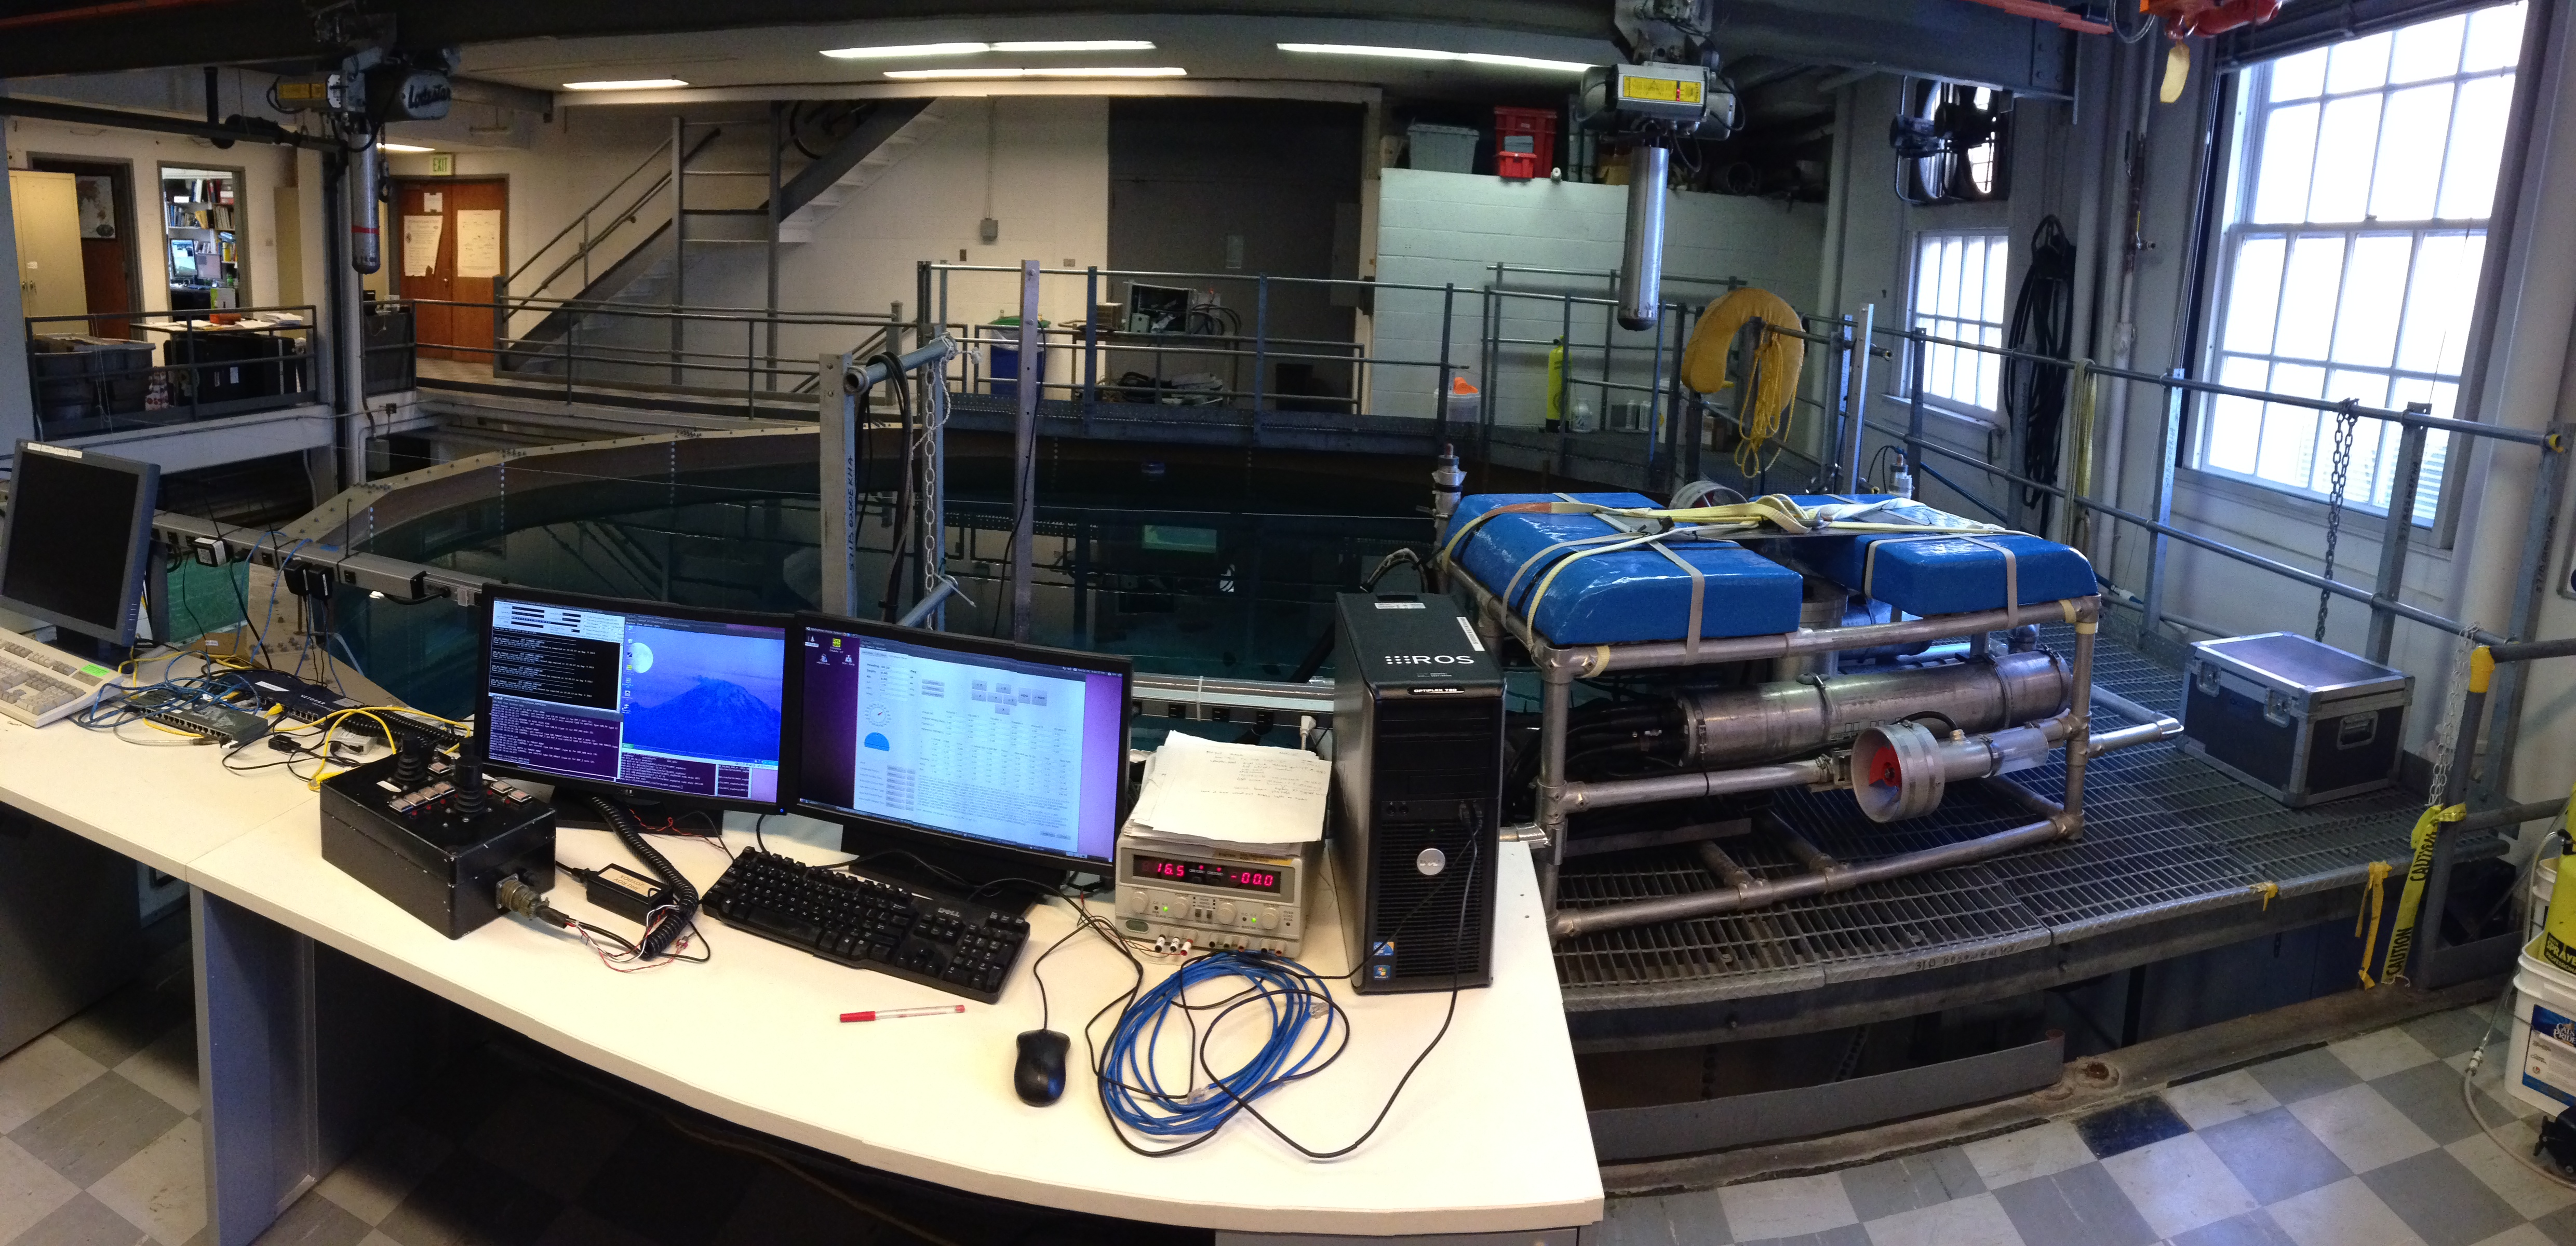
\includegraphics[trim=0mm 10cm 0mm 25cm,clip=true,width=\textwidth]{./appenJHUHTF/images/hydroFacility}
}
\\
\subfigure[\ac{JHUROV} starboard side view]  
{
    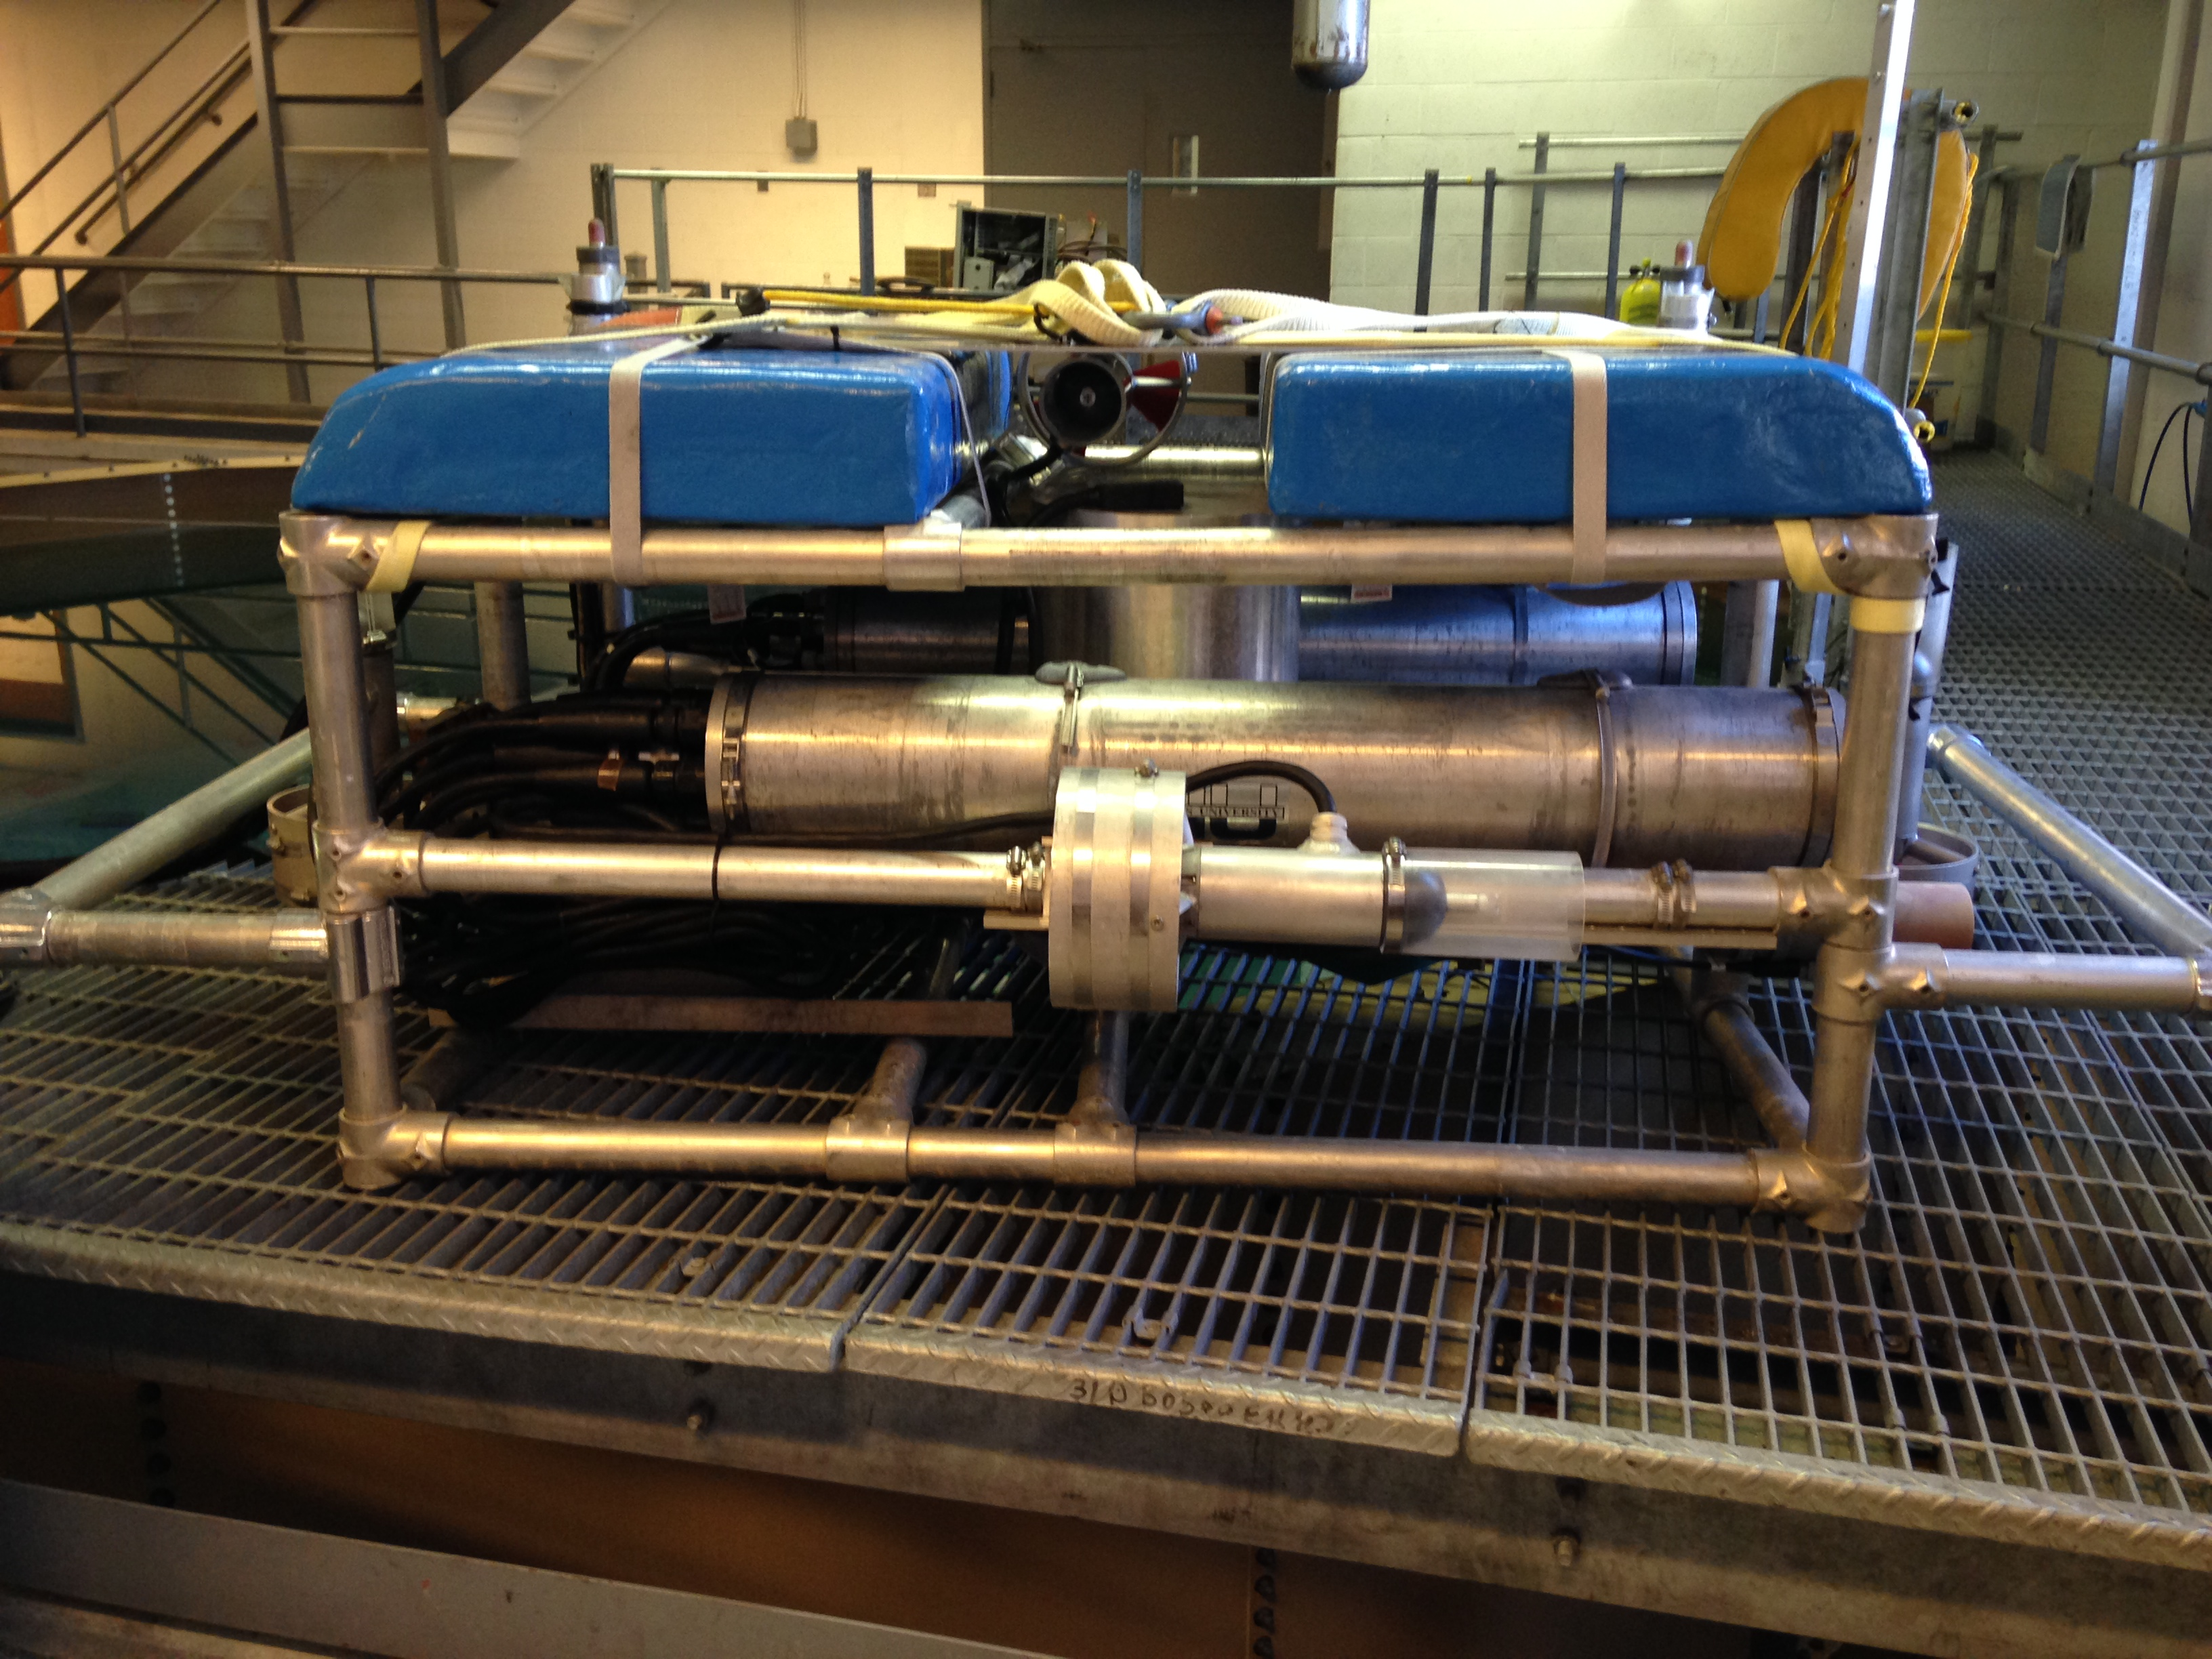
\includegraphics[trim=0mm 20cm 0mm 125mm,clip=true,width=.56\textwidth]{./appenJHUHTF/images/jhurovStarboard}
    %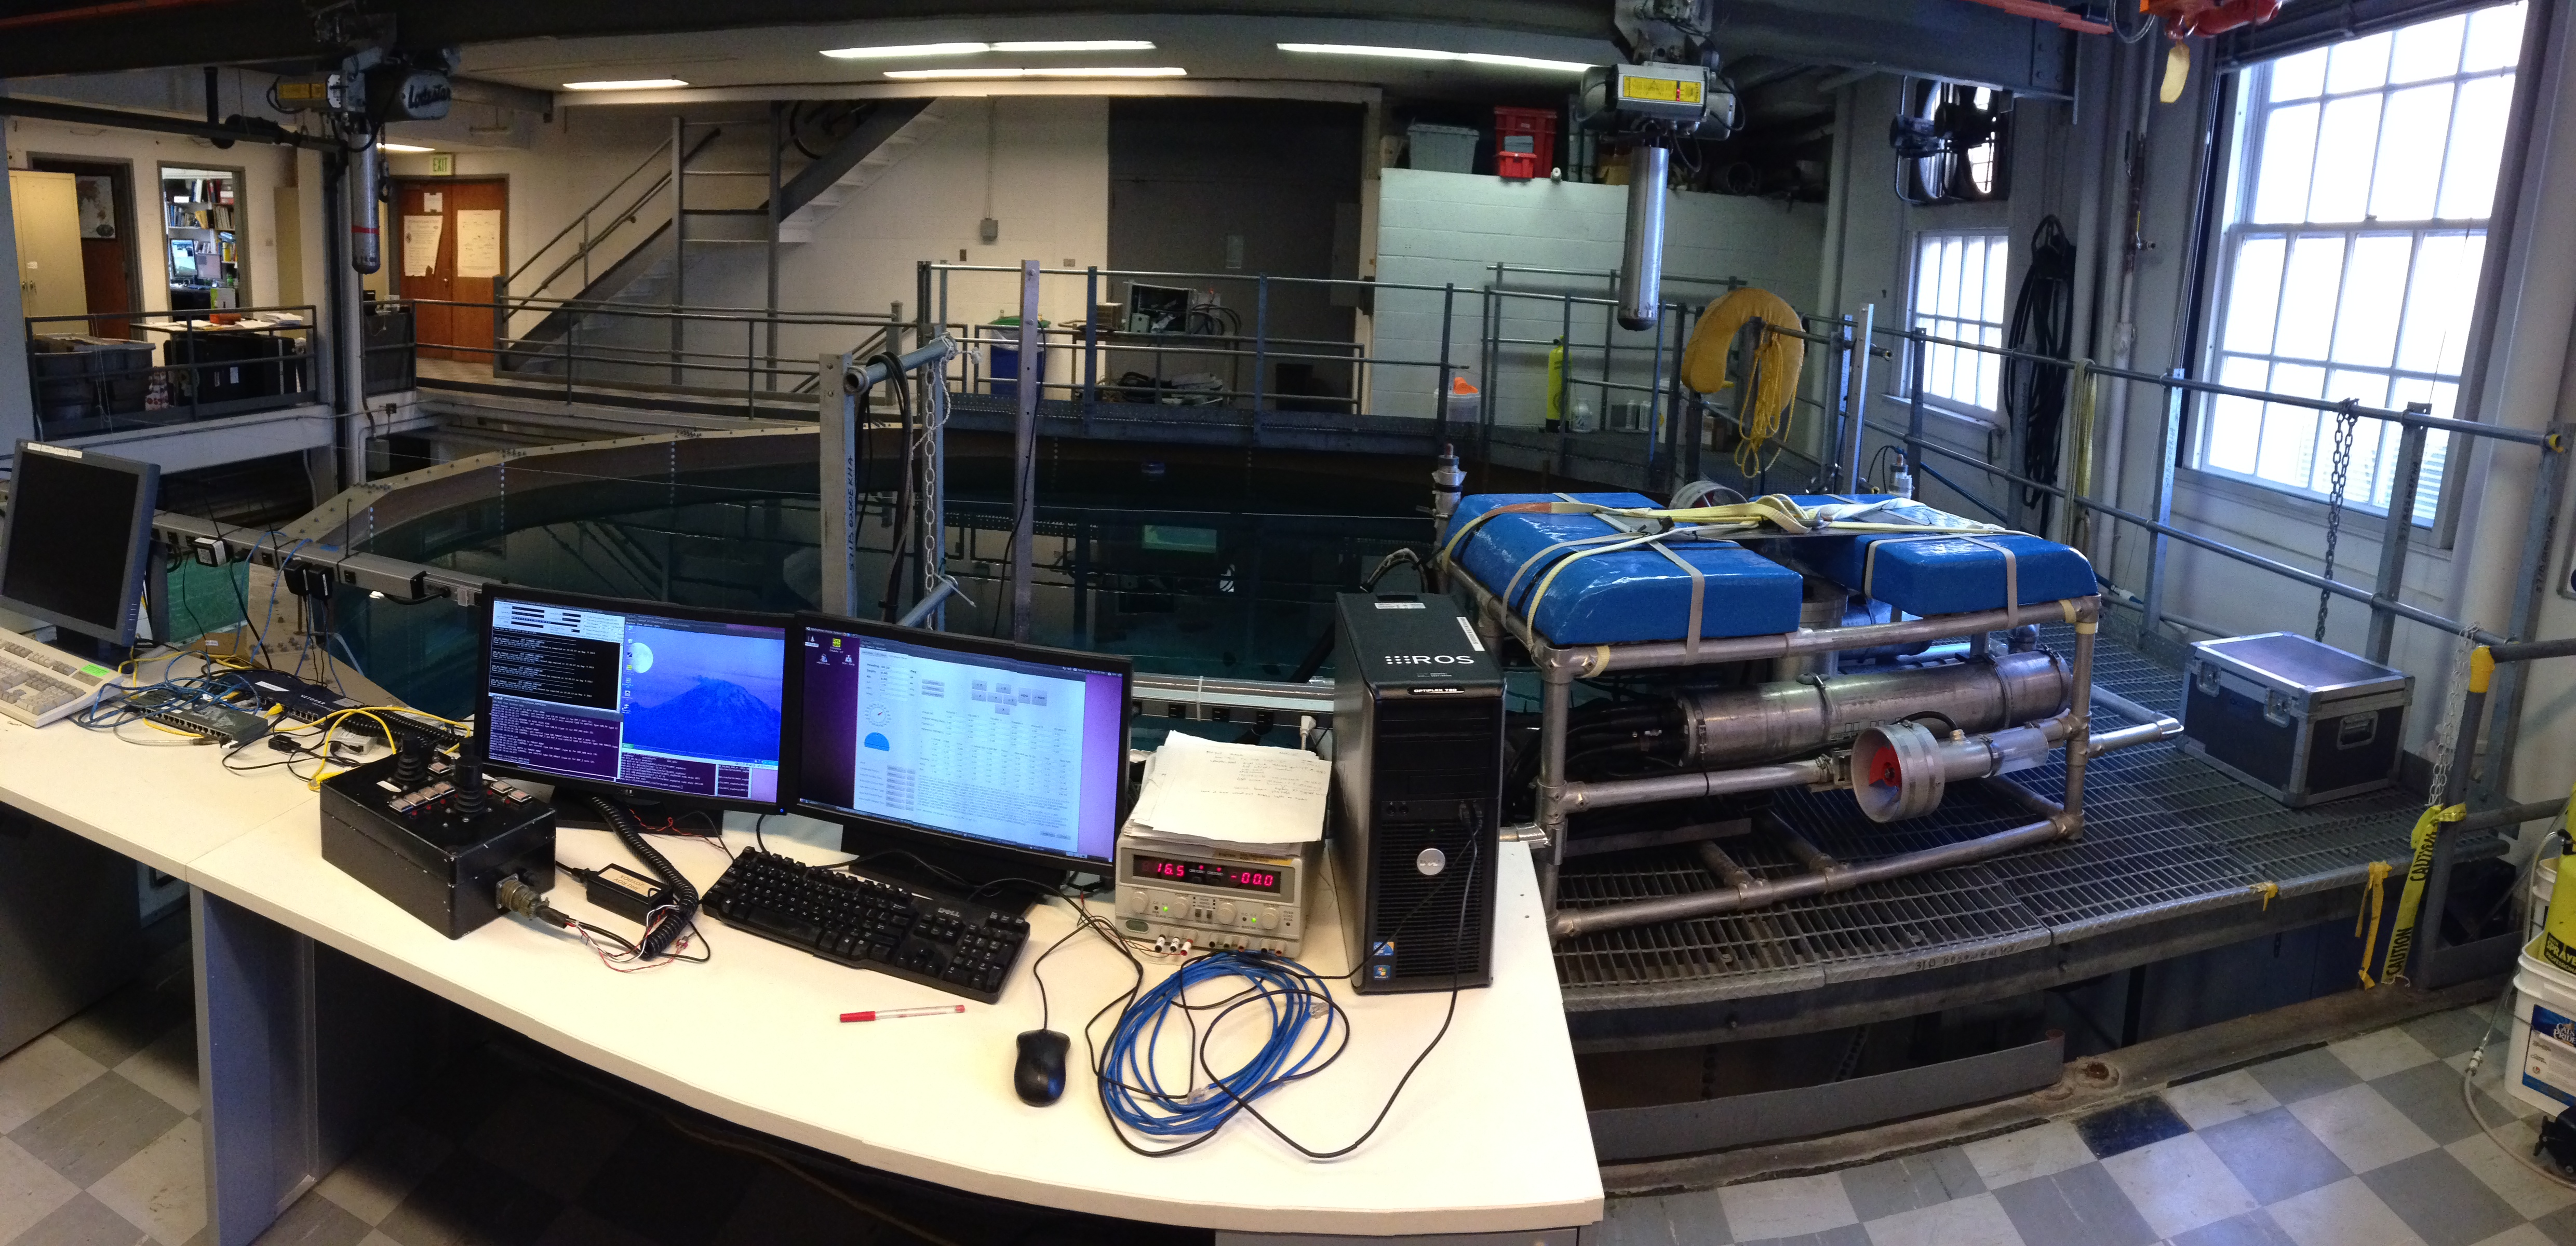
\includegraphics[width=170mm]{./appenJHUHTF/images/hydroFacility}
}
\subfigure[\ac{JHUROV} stern view] 
{
    %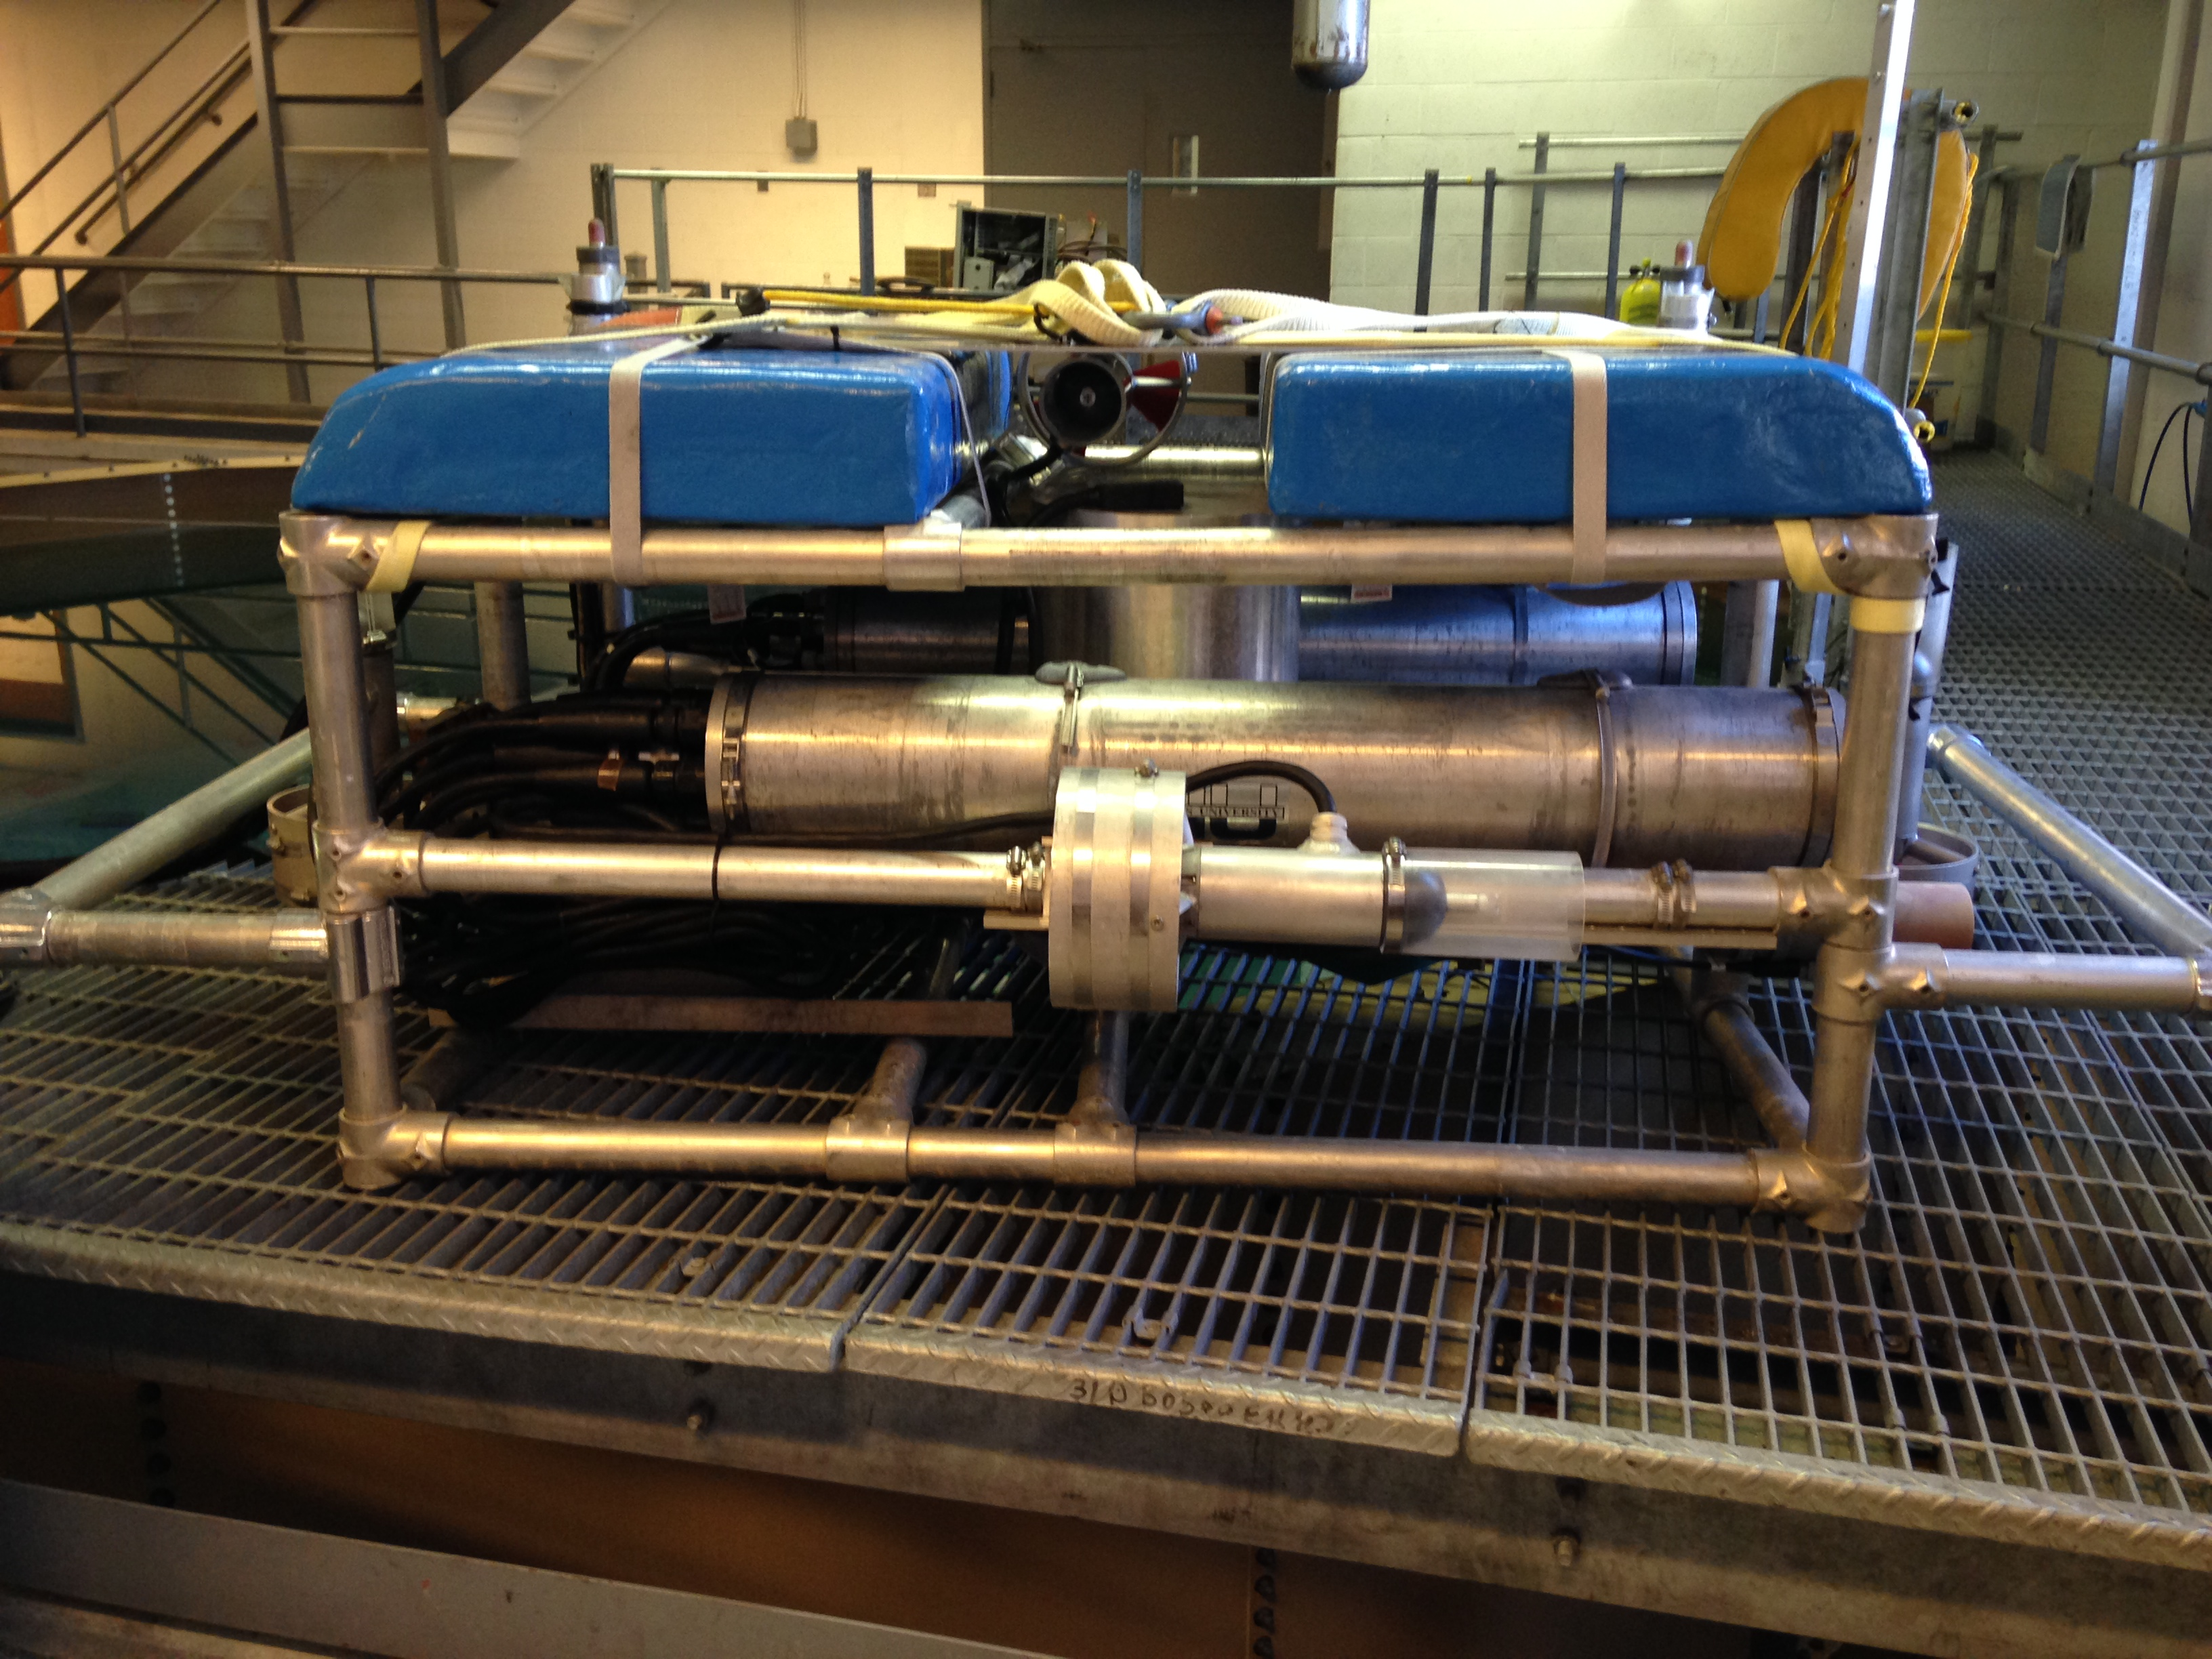
\includegraphics[trim=20cm 0mm 0mm 20cm,clip=true,width=80mm]{./appenJHUHTF/images/jhurovStarboard}
    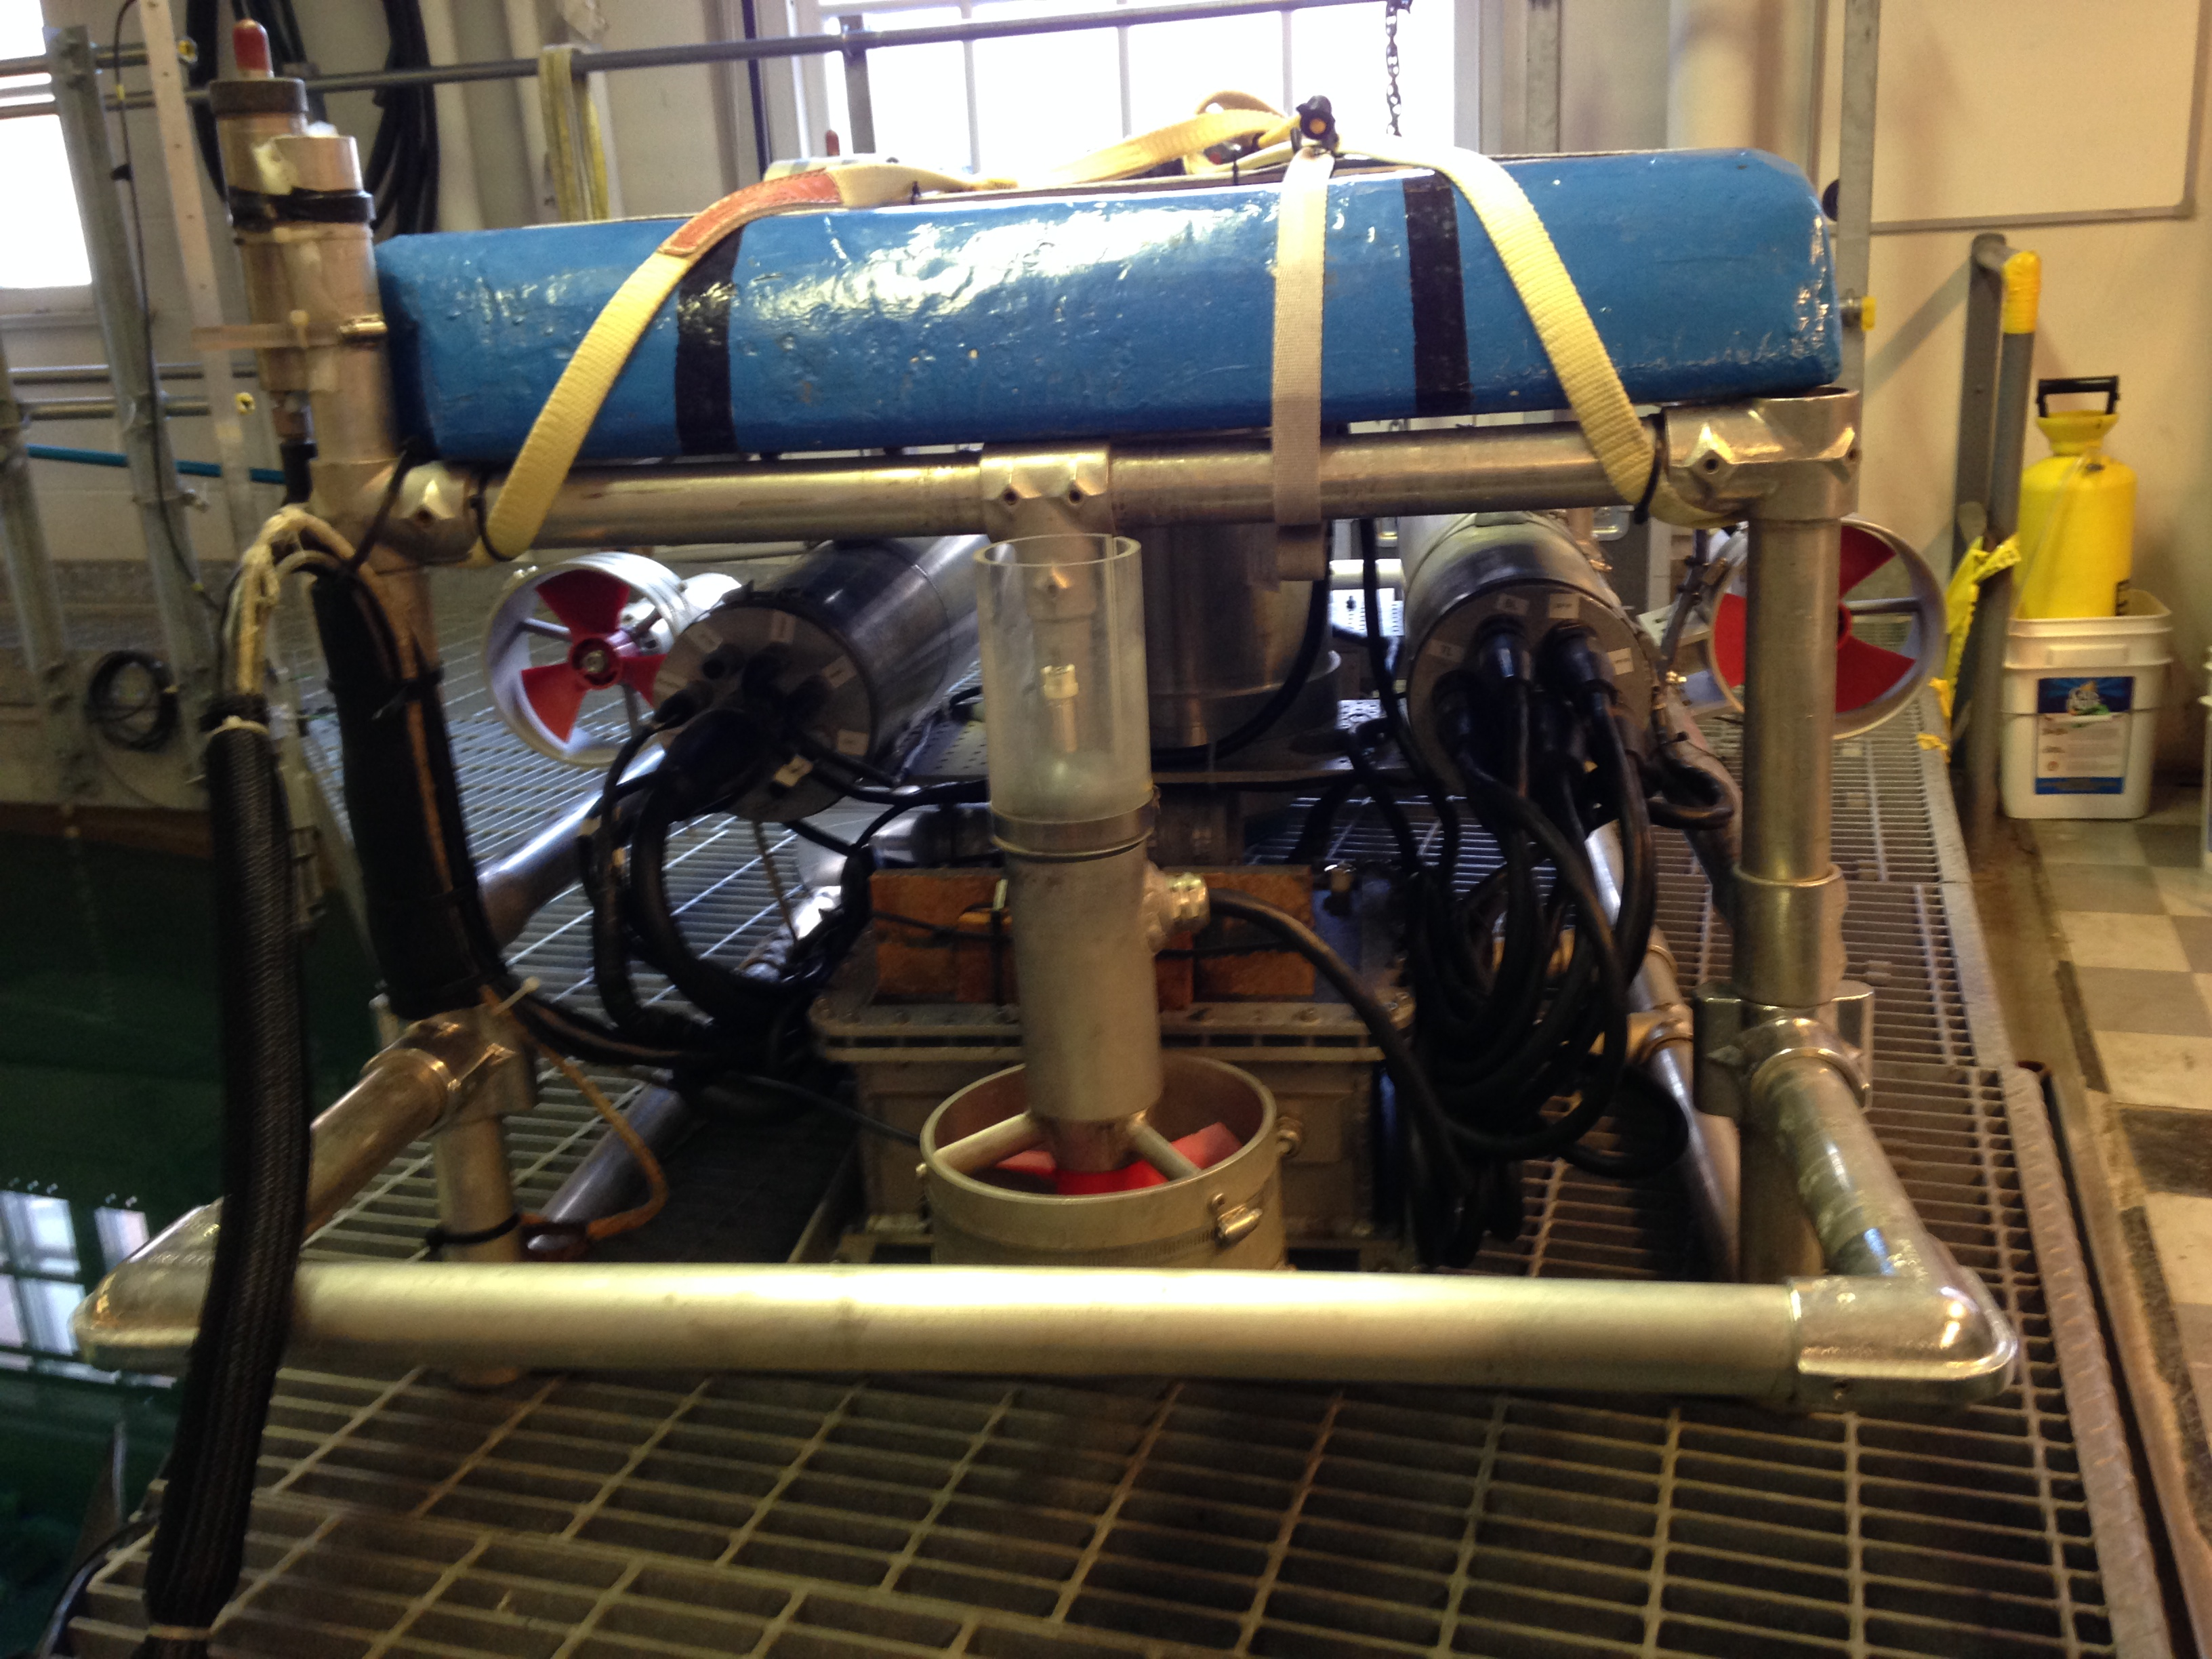
\includegraphics[trim=0mm 75mm 0mm 65mm,clip=true,width=.42\textwidth]{./appenJHUHTF/images/jhurovStern}
}
\caption{Johns Hopkins University Hydrodynamic Test Facility and \acf{JHUROV}.}
    \label{appenJHUHTF.fig.hydrolab}
\end{figure}
\end{center}


The Johns Hopkins Hydrodynamic Test Facility\cite{kinsey2003}
contains an indoor fresh water tank measuring \unit{7.75}{\m} in
diameter and \unit{4.25}{\m} deep, as shown in Figure
\ref{appenJHUHTF.fig.hydrolab}.  The facility is equipped with the
\ac{JHUROV}, a fully instrumented \ac{UV} designed for navigation and
control research.  The \ac{JHUROV} displaces \unit{150}{\kg} and is
actuated by six \unit{1.5}{\kWh} DC brushless electric direct drive
thrusters providing full control authority for 6-\ac{DOF}
maneuvers. Each thruster is controlled with a current-mode amplifier.
The \ac{JHUROV} control system generates the command current for each
thruster using data from {\it a-priori} {\it steady-state} thruster
calibration experiments; no feedback is used in generating the
commanded current.  The angular velocity of each thruster is
instrumented. This measured thruster angular velocity ($\omega_{th}$)
can be used to estimate the thruster force ($f_{th}$) using the
empirically validated steady state relation
$f_{th}=k_{th}\omega_{th}|\omega_{th}|$, where $k_{th}$ is an
empirically identified constant\cite{pona.book}.
%
The vehicle's control system is capable of actively controlling
6-\ac{DOF} vehicle motion.
%
During an experiment, each of the 6 \ac{JHUROV} \ac{DOF} were
independently actuated using either closed-loop control or open-loop
sinusoidal commanded torques. 
%
For the \acp{DOF} using closed-loop control,
a sinusoidal reference trajectory was specified to the \ac{JHUROV} control
system.



\begin{center}
\begin{figure}[htbp]
  \begin{center}
    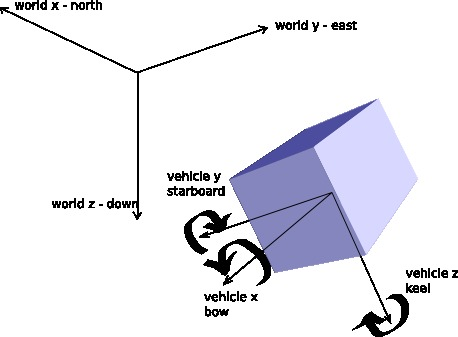
\includegraphics[width=90mm]{./appenJHUHTF/images/refFrames}
  \end{center}
  \caption{ The world-frame's orthonormal x, y, and z basis vectors
    point from the frame's origin towards in the directions north,
    east, and down respectively. The body-frame's orthonormal x, y, and
    z basis vectors point from the vehicles origin to the vehicle's
    bow side, starboard side and keel location respectively. Note the
    arrows showing positive rotation about each body axis.}
  \label{appenJHUHTF.fig.refFrames}
\end{figure}
\end{center}


The coordinate frames employed herein are depicted in Figure
\ref{appenJHUHTF.fig.refFrames}.
%
The world-frame's orthonormal x, y, and z basis vectors point from the
frame's origin towards the direction north, east, and down
respectively.
%
Employing standard navel architecture conventions, the body-frame's
orthonormal x, y, and z basis vectors point, respectively, from the
vehicle's origin to the vehicle's bow, starboard side and keel.
%
The Euler angles heading, pitch, and roll express the relationship
between the world-frame and body-frame as follows: rotating the world-frame
about its +z-axis through an angle heading, then rotating the resulting
frame about its +y-axis through an angle pitch, then rotating the
resulting-frame around its +x-axis through an angle roll provides the
body-frame.


\begin{table}[htbp]
\ssp
\caption{\ac{JHUROV} state measurement sources, resolutions, and accuracies}
\begin{center}
\begin{tabular}{cccc}
% & & RefTraj1& RefTraj2 \\
%\hline
%\multicolumn{2}{c}{Reference Trajectory}  &Trajectory Control      &  Parameter \\
%\multicolumn{2}{c}{Purpose}              & Evaluation &  Cross-Validation \\
 & &  & Measurement \\
State & Source  & Update Rate &Precision/Std Dev  \\
& & &(Standard Deviation)\\
\hline\hline
XY Translational  & DVLNAV    & \unit{10}{\Hz} & Resolution $>$0.5\% of\\
Position & & &Translational Distance Traveled \\
\hline
Z Translational   & Digiquartz & \unit{7}{\Hz} & Resolution \\
Position & & & $>$0.75\% as calculated \\
\hline
Heading                 & PHINS III & \unit{10}{\Hz}& 0.13$^\circ$ Std Dev \\  
\hline
Pitch, Roll             & PHINS III & \unit{10}{\Hz}& 0.01$^\circ$ Std Dev \\  
\hline
Translational  & \unit{1200}{\kHz}  & \unit{6}{\Hz} & $>$0.003 m/s Std Dev \\  
Velocity & \acs{DVL}& & \\
\hline
Angular Velocity        & PHINS III & \unit{10}{\Hz}& 0.01$^\circ$/s Std Dev \\  
\hline \hline\end{tabular}
\end{center}
\label{appen_JHUHTF.tb.sensors}
%\vspace*{-5mm}
\end{table}


The sensors used in all experimental evaluations are recorded in Table
\ref{appen_JHUHTF.tb.sensors}.  
%
The \ac{JHUROV} is instrumented by a PHINS III \ac{INS} (IXSEA SAS,
Marly-le-Roi, France), \unit{1200}{\kHz} bottom-lock Doppler sonar (RD
Instruments, San Diego, CA), and 8CDP010-1 Digiquartz Depth Sensor
(Paroscientific Inc., Redmond, WA).  
%
The PHINS III \ac{INS} includes a three-axis north-seeking fiber-optic
gyrocompass, and inertial grade accelerometers whose data is used to
estimate angular velocity, pitch, roll, and heading states at a rate
of \unit{10}{\Hz}.  
%
For our PHINS configuration, the measurement error standard deviations
are 0.01$^\circ$/s for angular velocity estimates, 0.13$^\circ$ for
heading estimates, and 0.01$^\circ$ for pitch and roll
estimates\cite{PhinsManual2008}. The Doppler sonar measures the three
dimensional linear velocity in the instrument's frame with a standard
deviation of less than 0.003 m/s, an update rate of \unit{6}{\Hz}, and
zero bias\cite{NWHdataSheet}.
%
The Digiquartz has a maximum depth of 10 m and, as currently
configured, has an update rate of \unit{7}{\Hz}, and provides pressure
measurements at a resolution of 2 parts-per-million.
%
Translational position estimates are provided by the DVLNAV control
software which integrates the the sensor signals reported above to
provide dead reckoning XY translational position estimates better than
0.5\% of distance traveled.
%








\section{Parameter Identification Evaluation}
\label{appenJHUHTF.sec.paramEvalMethod}

To evaluate the performance of the identified plant models we employ
an approach that we refer to as {\it cross-validation}.  
% 
We use the plant model experimentally identified from one vehicle
experimental trial to predict, in a numerical simulation, the
performance of the plant in a different experimental trial
whose trajectories differ from the identification trial.
%
The class of plants given by (\ref{chModels.eq.UVSO3plant}) and
(\ref{chModels.eq.UVSE3plant}) are open-loop-stable in their velocity
signals as a consequence of hydrodynamic damping. 
%
In the presence of significant buoyancy torque due to
\ac{COB} to \ac{COG} separation, both classes of
plants are also open-loop-stable in roll and pitch.
%
Because these open-loop signals are stable, we can employ these
signals to compare a model plant's predicted performance to the
actual plant's experimentally observed performance.
% 
The error between the predicted model performance and the
experimentally observed performance is reported as the \ac{MAE}
between the simulated plant roll, pitch, and velocity and the actual
experimental plant roll, pitch, and velocity.



%\section{Trajectory Tracking Evaluation}
\label{appenJHUHTF.sec.trajTrackEvalMethod}

To compare the trajectory tracking performance of controllers we
consider the \ac{MNE}, such as the position
and velocity error vectors.
%
A smaller \ac{MNE} value means the controller is doing a better job
tracking the reference trajectory.


\chapter{SE(3) Velocity Jacobian}
\label{appenJacSE3}
\chaptermark{SE(3) Velocity Jacobian}
%\ssp
\acresetall


This Section derives several facts about the inverse SE(3) velocity
Jacobian.  This matrix valued function,
\funDefn{\hat{\mathcal{A}}^{-1}}{\rSp{6}}{\rSp{6\times 6}}, relates
the body-frame velocity and time derivative of exponential coordinate
pose by the equality
%
\begin{equation}
\dot{\psi}=\hat{\mathcal{A}}^{-1}(\psi) v.
\end{equation}
%
In \cite{bullo1995_SE3_PD} the authors derive the following closed
form equation for this matrix valued function
%
% \begin{equation}\label{appenJacSE3.eq.hatAinv}
%   \hat{\mathcal{A}}^{-1}\left(\left[ \begin{array}{c} 
% \xi \\ q  \\
% \end{array} \right]\right)=
%     I_{6\times 6}+\frac{1}{2}\ad\left(\left[ \begin{array}{c} 
% \xi \\ q  \\
% \end{array} \right]\right)
% +\mathbb{B}_1\left(\|q\|\right)\ad^2\left(\left[ \begin{array}{c} 
% \xi \\ q  \\
% \end{array} \right]\right)+\mathbb{B}_2\left(\|q\|\right)\ad^4\left(\left[ \begin{array}{c} 
% \xi \\ q  \\
% \end{array} \right]\right)
% \end{equation}
% %
% where 
% %
% \begin{equation}
% y^2 \mathbb{B}_1\left( y \right)=2\left(1-\alpha(y))\right)+\frac{1}{2}\left(\alpha(y)-\beta(y)\right)
% \end{equation}
% %
% \begin{equation}
% y^4 \mathbb{B}_2\left( y \right)=\left(1-\alpha(y))\right)+\frac{1}{2}\left(\alpha(y)-\beta(y)\right)
% \end{equation}
% %
% with $\alpha(y)=\frac{y}{2}\cot\left( \frac{y}{2}\right)$
% and $\beta(y)=\left(\frac{y}{2}\right)^2\frac{1}{\sin\left(\frac{y}{2}\right)}$.
% Using the fact that $\mathcal{J}(q)^3=-\|q\|^2 \mathcal{J}(q)$,
% (\ref{appenJacSE3.eq.hatAinv}) can be show to be equivalent to
% %
% \begin{equation}
%    \hat{\mathcal{A}}^{-1}\left(\left[ \begin{array}{c} 
% \xi \\ q  \\
% \end{array} \right]\right)=
% \left[ \begin{array}{cc}
%      \mathcal{A}^{-1}(q) &  \frac{1}{2}\soThreeMap{\xi} + 
%                            \frac{1-\alpha(\|q\|)}{\|q\|^2}\left(\soThreeMap{\xi}\soThreeMap{q}+\soThreeMap{q}\soThreeMap{\xi}\right)+ 
%                            \mathcal{B}_2(\|q\|)\mathcal{B}_3\left( \xi, q\right)   \\
%       0_{3 \times 3}     & \mathcal{A}^{-1}(q)    \\
% \end{array} \right]
% \end{equation}
% %
% where 
% \funDefn{ \mathcal{B}_3 }{ \rSp{3}\times\rSp{3} }{\rSp{3\times 3}} is defined by 
% $\mathcal{B}_3(\xi,q)=\soThreeMap{q}\soThreeMap{\xi}\soThreeMap{q}^2+\soThreeMap{q}^2\soThreeMap{\xi}\soThreeMap{q}$.  
% %
% To the best of our knowledge a closed form expression for the SE(3)
% angular velocity jacobian, $\hat{\mathcal{A}}\left(\psi\right)$, has
% not been previously reported.
%
% %--------------------------
% \subsubsection{devider}
%
\begin{equation}\label{appenJacSE3.eq.hatAinv}
  \hat{\mathcal{A}}^{-1}\left(\left[ \begin{array}{c} 
        \xi \\ q  \\
\end{array} \right]\right)=
    I_{6\times 6}+\frac{1}{2}\ad\left(\left[ \begin{array}{c} 
\xi \\ q  \\
\end{array} \right]\right)
+\mathcal{B}_1\left(\|q\|\right)\ad^2\left(\left[ \begin{array}{c} 
\xi \\ q  \\
\end{array} \right]\right)+\mathcal{B}_2\left(\|q\|\right)\ad^4\left(\left[ \begin{array}{c} 
\xi \\ q  \\
\end{array} \right]\right)
\end{equation}
%
where 
%
\begin{equation}
y^2 \mathcal{B}_1\left( y \right)=2\left(1-\alpha(y)\right)+\frac{1}{2}\left(\alpha(y)-\beta(y)\right)
\end{equation}
%
\begin{equation}
y^4 \mathcal{B}_2\left( y \right)=\left(1-\alpha(y)\right)+\frac{1}{2}\left(\alpha(y)-\beta(y)\right)
\end{equation}
%
with $\alpha(y)=\frac{y}{2}\cot\left( \frac{y}{2}\right)$
and $\beta(y)=\left(\frac{y}{2}\right)^2\frac{1}{\sin\left(\frac{y}{2}\right)^2}$.
Using the fact that $\mathcal{J}(q)^3=-\|q\|^2 \mathcal{J}(q)$,
(\ref{appenJacSE3.eq.hatAinv}) can be shown to be equivalent to
%
\begin{equation}\label{appenJacSE3.eq.hatAinv2} 
 \hat{\mathcal{A}}^{-1}\left(\left[ \begin{array}{c} 
\xi \\ q  \\
\end{array} \right]\right)
=\left[ \begin{array}{cc}
     \mathcal{A}^{-1}(q) &  \frac{1}{2}\soThreeMap{\xi} + 
                           \frac{1-\alpha(\|q\|)}{\|q\|^2}\mathcal{B}_4\left( \xi, q\right) 
                           +\mathcal{B}_2(\|q\|)\mathcal{B}_3\left( \xi, q\right)   \\
      0_{3 \times 3}     & \mathcal{A}^{-1}(q)    \\
\end{array} \right]
\end{equation}
%
\noindent where 
\funDefn{ \mathcal{B}_4 }{
  \realSpace{3}\times\realSpace{3} }{\realSpace{3\times 3}} is defined by
$\mathcal{B}_4(\xi,q)=\soThreeMap{\xi}\soThreeMap{q}+\soThreeMap{q}\soThreeMap{\xi}$ and
\funDefn{ \mathcal{B}_3 }{
  \realSpace{3}\times\realSpace{3} }{\realSpace{3\times 3}} is defined
by
$\mathcal{B}_3(\xi,q)=\soThreeMap{q}\soThreeMap{\xi}\soThreeMap{q}^2+\soThreeMap{q}^2\soThreeMap{\xi}\soThreeMap{q}$.
To the best of the author's knowledge a closed form expression for the
SE(3) velocity Jacobian, $\hat{\mathcal{A}}\left(\psi\right)$,
has not been reported.  

\section{SE(3) Velocity Jacobian Bilinear se(3) Pose Multiplication Simplification}
\label{appenJacSE3.sec.PsiHatAinvPsiEquality}

In this Section we prove
%
\begin{equation}\label{appenJacSE3.eq.PsiHatAinvPsiEquality}
\psi^T\left(\hat{\mathcal{A}}^{-T}(\psi)+\hat{\mathcal{A}}^{-1}(\psi)\right)\psi=\psi^T\psi.
\end{equation}
%
Consider inserting (\ref{appenJacSE3.eq.hatAinv2}) into the left side
of (\ref{appenJacSE3.eq.PsiHatAinvPsiEquality}).  
%
Note that the definition of $\mathcal{A}^{-1}$ in (\ref{chModels.eq.Ainv}) and
$\soThreeMap{q}q=\vec{0}$ imply the following facts:
\begin{itemize}
\item$\mathcal{A}^{-1}(q)q=q$,
\item$\frac{1-\alpha(\|q\|)}{\|q\|^2}\soThreeMap{\xi}\soThreeMap{q}q=\vec{0}$, and
\item $\mathcal{B}_2(\|q\|)\mathcal{B}_3\left( \xi, q\right)q=\vec{0}$.
\end{itemize}
%
These facts imply
%
\begin{equation}
\psi^T\left(\hat{\mathcal{A}}^{-1}(\psi)\right)\psi=\psi^T
\left[ \begin{array}{cc}
     \mathcal{A}^{-1}(q) & \frac{1-\alpha(\|q\|)}{\|q\|^2}\soThreeMap{q}\soThreeMap{\xi} \\
      0_{3 \times 3}     & 0_{3 \times 3}   \\
\end{array} \right]\psi.
\end{equation}
%
From which we can see
%
\begin{align}
\frac{1}{2}\psi^T\left(\hat{\mathcal{A}}^{-1}(\psi)+\hat{\mathcal{A}}^{-T}(\psi)\right)\psi
%\nonumber \\
=&\frac{1}{2}\xi^T\left(\mathcal{A}^{-1}(q)+\mathcal{A}^{-T}(q)\right)\xi+
\nonumber \\
&\frac{1-\alpha(\|q\|)}{2 \|q\|^2}\left(\xi^T\soThreeMap{q}\soThreeMap{\xi}q+
q^T \soThreeMap{\xi}\soThreeMap{q}\xi\right)+q^Tq
\nonumber \\
=&\xi^T \xi+q^T q+
\nonumber \\
 &\frac{1-\alpha(\|q\|)}{2 \|q\|^2}\left(2\xi^T \soThreeMap{q}^2 \xi- 
2\xi^T \soThreeMap{q}\soThreeMap{q}\xi\right)
\nonumber \\
=&\psi^T\psi
\nonumber
\end{align}
%
%This equality is required to prove Theorem
%\ref{chUV_AMBC.theo.UV_MBC}
\section{Bounding $\|\hat{\mathcal{A}}^{-1}(\psi)x\|$}
\label{appenJacSE3.sec.normBound}

In this Section we show there $\exists c\in\rSp{}_+$ such
that $\forall\psi,x\in\rSp{6}$ for which $\|\psi\|<\pi$ we have
$\|\hat{\mathcal{A}}^{-1}(\psi)x\| <c\|x\|$.
%
Specifically, we prove  $c=6+\frac{5\pi}{2}+\frac{\pi^2}{8}$ satisfies this
inequality. %, though it is likely not the minimum value which does so.
%
Let $\xi,\;q,\;x_1\;x_2\in\rSp{3}$ such that
$\psi=[\xi^T \quad q^T ]^T$ and
$x=[ x_1^T \quad x_2^T ]^T$, then
%$x=\left[ \begin{array}{c} x_1 \\ x_2 \end{array} \right]$, then
%
\begin{align}
\|\hat{\mathcal{A}}^{-1}(\psi)x\|\leq&\|\mathcal{A}^{-1}(q)x_1\|+\|\mathcal{A}^{-1}(q)x_2\|
\nonumber \\
    &+\|\left( \frac{1}{2}\soThreeMap{\xi} + 
                           \frac{1-\alpha(\|q\|)}{\|q\|^2}\mathcal{B}_4\left( \xi, q\right) 
                           +\mathcal{B}_2(\|q\|)\mathcal{B}_3\left( \xi, q\right)   \right)x_2\|.
\label{appenJacSE3.eq.interimBound}
\end{align}
%
Note that $\|x_1\|\leq\|x\|$, $\|x_2\|\leq\|x\|$,
$\|\xi\|\leq\|\psi\|<\pi$, and $\|q\|\leq\|\psi\|<\pi$. Consider
%
\begin{align}
\|\mathcal{A}^{-1}(q)x_i\|
   \leq&\|x_i\|+\|\soThreeMap{q}x_i\|+
        \|\left(1-\alpha(\|q\|)\right)\frac{\soThreeMap{q}^2}{\|q\|^2}x_i\|
\nonumber \\
   \leq&\|x_i\|+\|q\|\|x_i\|+
        |\left(1-\alpha(\|q\|)\right)|\;\|x_i\|.
\end{align}
%
For $q$ such that $\|q\|<\pi$ consider the value of
$|(1-\alpha(\|q\|)|$.  Note that 
for $y=\frac{\pi}{2}$ we know $1-y\cot(y)=1$;  by l'Hospital's rule we know
%
$\lim_{y\rightarrow 0^+}y\cot(y)=\lim_{y\rightarrow 0^+}\frac{\cos(y)-y\sin(y)}{\cos(y)}=1$;
%
and for $y\in\left(0,\; \frac{\pi}{2} \right)$ we know
$\frac{d}{dy}\left(1-y\cot(y) \right)>0$.  These imply
$\forall y\in\left[0,\; \frac{\pi}{2} \right)\quad |1-y\cot(y)| \leq
1$ and therefore
$\|\mathcal{A}^{-1}(q)x_i\|<\left(2+\pi\right)\|x_i\|$.
%
%\begin{equation}
%\|\mathcal{A}^{-1}(q)x_i\|\leq\left(2+\pi\right)\|x_i\|
%\end{equation}
%

A similar analysis can be used to bound other terms in
(\ref{appenJacSE3.eq.interimBound}).  Using l'Hospital's rule and
differiation it can be shown $\lim_{y\rightarrow
  0^+}\frac{1-\alpha(y)}{y}=0$,
$\frac{1-\alpha(\pi)}{\pi}=\frac{1}{\pi}$, and the function
$\frac{1-\alpha(y)}{y}$ is strictly increasing for $y\in\left(0,\pi
\right)$; these facts and previous definitions are used to show
%
\begin{align}
\|\frac{1-\alpha(\|q\|)}{\|q\|^2}\mathcal{B}_4\left( \xi, q\right)x_2\|
   =&\|\frac{1-\alpha(\|q\|)}{\|q\|}\mathcal{B}_4\left( \xi,\frac{q}{\|q\|}\right)x_2\|
\nonumber \\
   \leq& |\frac{1-\alpha(\|q\|)}{\|q\|}|\;\|\xi\|\|x_2\|
\nonumber \\
   <&\|x_2\|.
\nonumber
\end{align}
%
Using l'Hospital's rule and differiation it can be shown
$\lim_{y\rightarrow 0^+}\frac{\alpha(y)-\beta(y)}{2y}=0$,
$\frac{\alpha(\pi)-\beta(\pi)}{2\pi}=\frac{-\pi}{8}$, and the function
$\frac{\alpha(y)-\beta(y)}{2y}$ is strictly decreasing for
$y\in\left(0,\pi \right)$; these facts and previous definitions are
used to show
%
\begin{align}
\|\mathcal{B}_2(\|q\|)\mathcal{B}_3\left( \xi, q\right)x_2\|
   =&\|\frac{(1-\alpha(\|q\|))+\frac{1}{2}(\alpha(\|q\|)
     -\beta(\|q\|))}{\|q\|}\mathcal{B}_3\left( \xi,\frac{q}{\|q\|}\right)x_2\|
\nonumber \\
   \leq& \left(|\frac{1-\alpha(\|q\|)}{\|q\|}|+|
         \frac{\alpha(\|q\|)-\beta(\|q\|)}{2\|q\|} |\right)\;\|\xi\| \|x_2\|
\nonumber \\
   <&\left(1+\frac{\pi^2}{8}\right)\|x_2\|.
\end{align}
%
Therefore, using the bounds above, from (\ref{appenJacSE3.eq.interimBound}) we have
%
\begin{align}
\|\hat{\mathcal{A}}^{-1}(\psi)x\|<& \left(2+\pi\right)\|x_1\|+\frac{1}{2}\|\xi\|\|x_2\|
            +\|x_2\|+\left(1+\frac{\pi^2}{8}\right)\|x_2\|+\left(2+\pi\right)\|x_2\|
\nonumber \\
     <& \left(6+\frac{5\pi}{2}+\frac{\pi^2}{8}\right)\|x\|
\end{align}

% \input{appKF.tex}
% \input{appIF.tex}
% \input{appIFex.tex}


%% REFERENCES
\bibliographystyle{sty/IEEEtranS}
\bibliography{tophrefs/new,tophrefs/sweb,tophrefs/iros2011,tophrefs/robot,tophrefs/rov,tophrefs/books,tophrefs/kod,tophrefs/llw} %tophrefs/bibs,tophrefs/jck,tophrefs/rme,

\begin{vita}

 \dssp
 \begin{wrapfigure}{l}{0pt}
   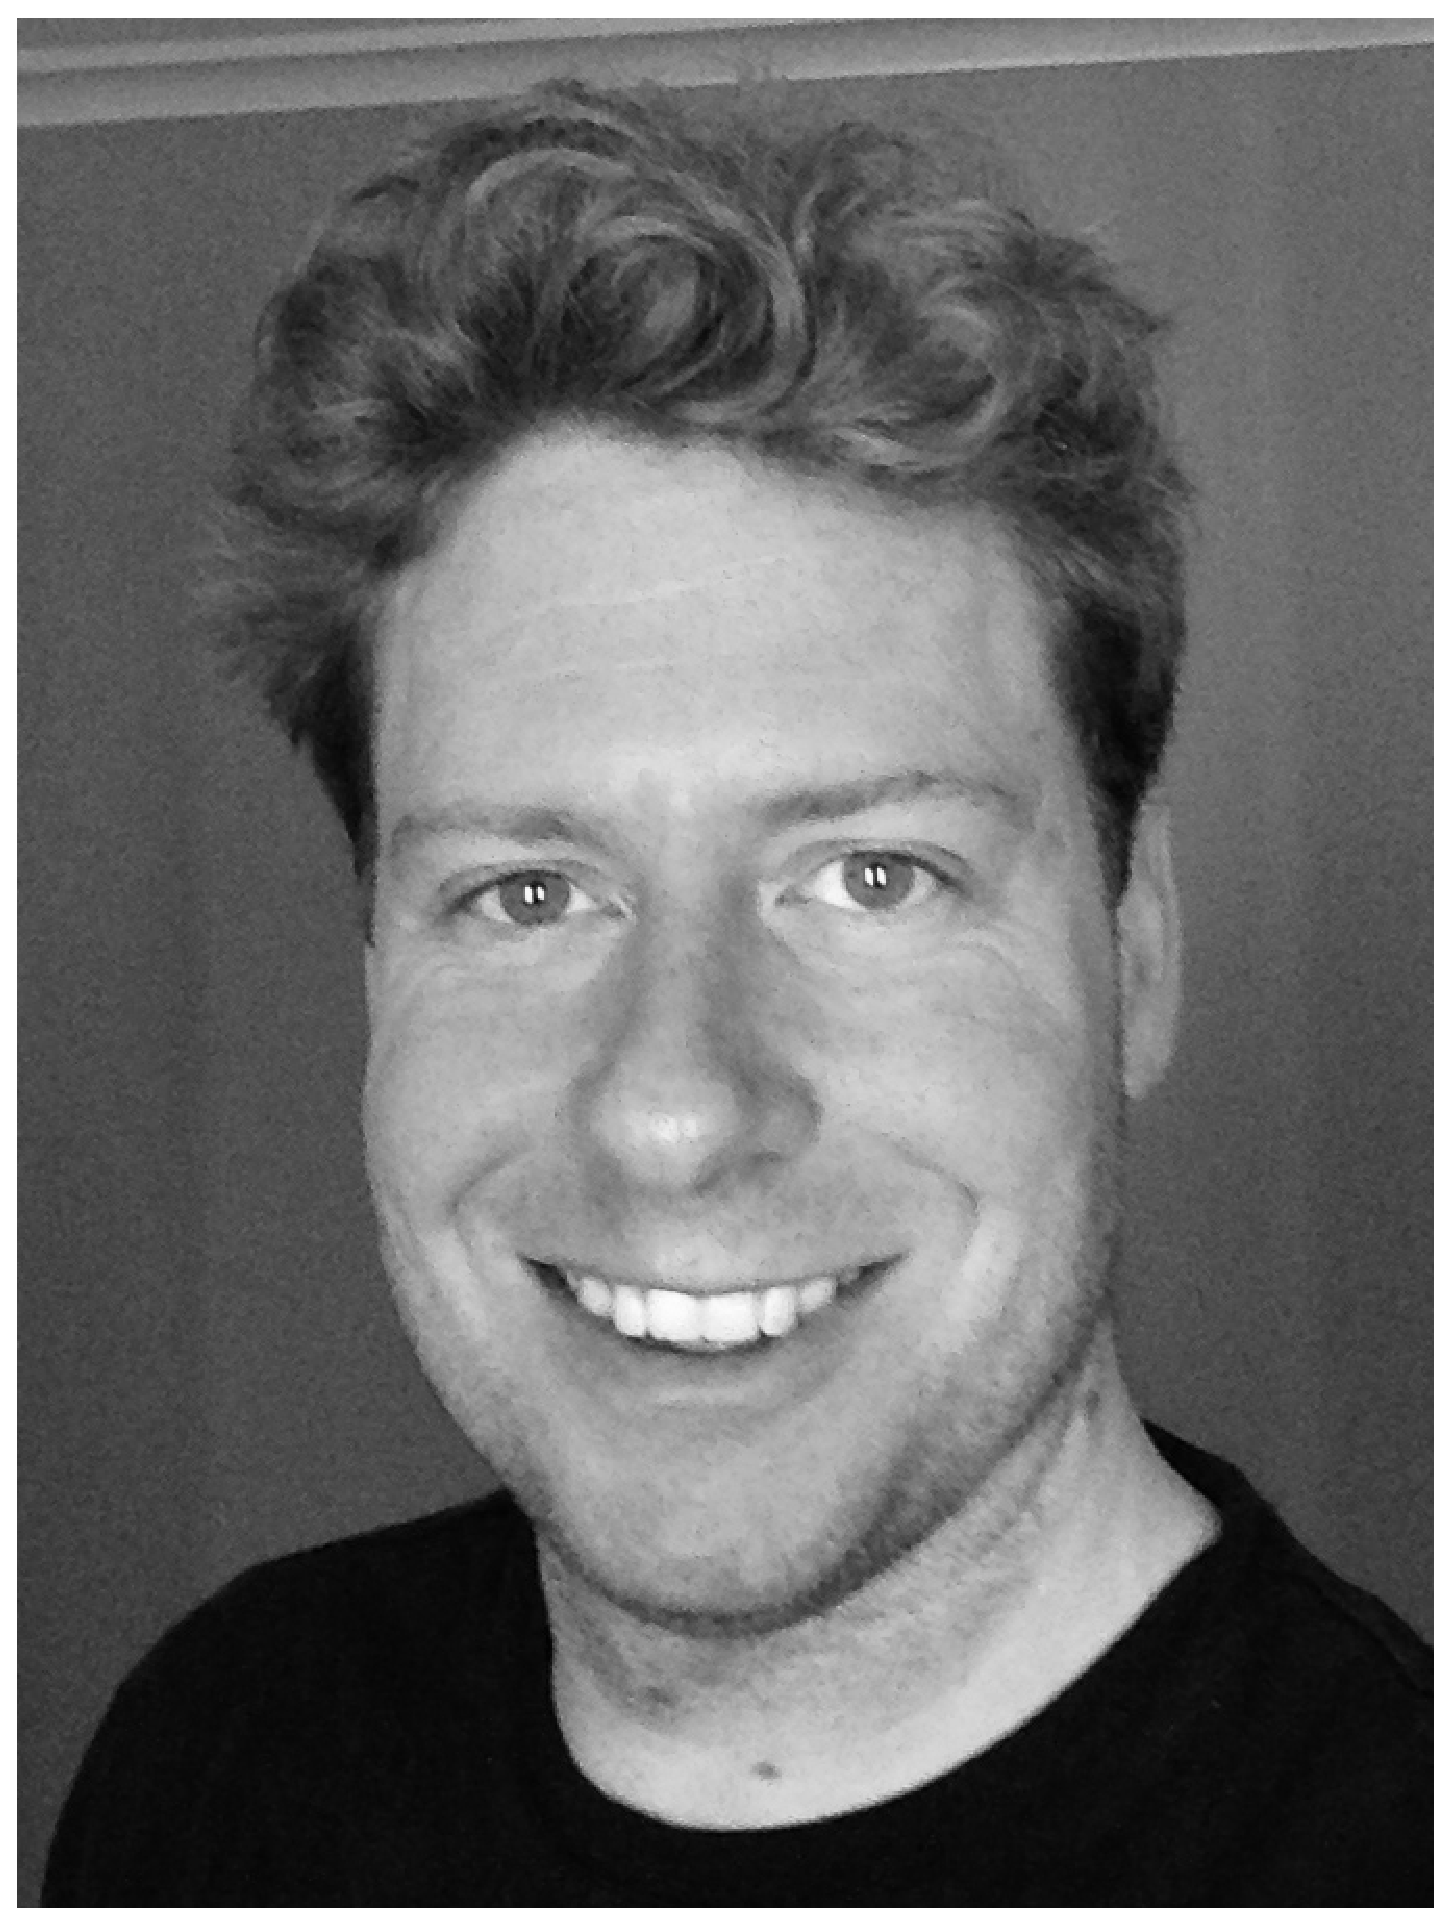
\includegraphics[width=1.5in]{toph_bwCrop}
 \end{wrapfigure}

 Christopher J. McFarland was born in Tulsa, Oklahoma in 1983.  From
 2002 to 2007 he participated in the Dual-Degree program between the
 University of Puget Sound in Tacoma, Washington and Washington
 University in St.\ Louis, Missouri.  Christopher attended both
 institutions, receiving both a \mbox{B.\ A.\ } in Physics with a minor in Math
 from the University of Puget Sound and a \mbox{B.\ S.\ } in Mechanical
 Engineering from Washington University in May 2007.  In August 2007
 he enrolled in the Mechanical Engineering Ph.D.\ program at Johns
 Hopkins University.

 Christopher has been recognized with several distinctions including
 Eagle Scout by the Boy Scouts of America in 2000; a Brown Fellowship
 for Dual-Degree Engineering Students from 2005-2007; NSF Graduate
 Research Fellowship honorable mention in 2007 and 2008; Johns Hopkins
 University Mechanical Engineering Department Fellowship 2007-2008;
 National Defense Science and Engineering Graduate Fellowship
 2008-2011; Link Foundation Doctoral Research Fellowship in Ocean
 Engineering and Instrumentation 2012-2013; and Achievement Rewards
 for College Scientists Fellowship 2012-2013.

\end{vita}

\end{document}
